\documentclass{article}

\usepackage[
  top=2cm,
  bottom=2cm,
  left=2cm,
  right=2cm,
  headheight=17pt, % as per the warning by fancyhdr
  includehead,includefoot,
  heightrounded, % to avoid spurious underfull messages
]{geometry} 
\usepackage{caption}
\usepackage[export]{adjustbox}
\usepackage{fancyhdr}
\pagestyle{fancy}
\usepackage{listings} %Para colcoar codigos
\usepackage[utf8]{inputenc}
\usepackage[spanish, mexico]{babel}
\usepackage{caption}
\usepackage{hyperref}
\usepackage[table,xcdraw]{xcolor}
\usepackage{graphicx}
\usepackage{float}
\usepackage{color}
\usepackage{subfigure}
\usepackage{array}
\usepackage{longtable}
\DeclareGraphicsExtensions{.pdf,.jpeg,.png,.eps,.jpg,.svg}
\usepackage{enumerate}
\usepackage{listings}
\usepackage{amsmath}
\usepackage{amssymb}
\usepackage{mathtools}
\usepackage{mathrsfs}
\usepackage{enumitem}
\usepackage[numbers,sort&compress]{natbib}

\usepackage{xr}
\usepackage{pdfpages}
\usepackage[normalem]{ulem}
\PassOptionsToPackage{subfigure}{tocloft}
\usepackage{fixmetodonotes}
\usepackage[T1]{fontenc}
\usepackage{xcolor}
\usepackage{graphicx,import}
\usepackage{cmap}
\usepackage{hyperref}
\renewcommand{\lstlistingname}{Código}
\renewcommand{\lstlistlistingname}{Indice de códigos}

\definecolor{codegreen}{rgb}{0,0.6,0}

\useunder{\uline}{\ul}{}

\lstdefinestyle{customc}
{
  belowcaptionskip=1\baselineskip,
  breaklines=true,
  frame=L,
  xleftmargin=\parindent,
  language=Matlab,
  showstringspaces=false,
  basicstyle=\footnotesize\ttfamily,
  keywordstyle=\bfseries\color{green!40!black},
  commentstyle=\itshape\color{purple!40!black},
  identifierstyle=\color{black},
  stringstyle=\color{orange},
   commentstyle=\color{codegreen},
}

\newcommand{\subsubsubsection}[1]{\paragraph{#1}\mbox{}\\}
\setcounter{secnumdepth}{4}
\setcounter{tocdepth}{4}

\rhead{Proyecto MEDICI - UniAndes}
\lhead{Informe de Avance Proyecto Especial y Tesis I}
\setlength{\parskip}{1em}
\lstset{style=customc}

\begin{document}

\lstset{
	basicstyle=\ttfamily\fontfamily{iwona}\tiny\scriptsize,
	frame=single,
	showspaces=false, % show spaces adding particular underscores
	showstringspaces=false, % underline spaces within strings
	showtabs=false, % show tabs within strings adding particular underscores
	tabsize=1, % sets default tabsize to 2 spaces
	captionpos=true, % sets the caption-position to bottom
	breaklines=true, % sets automatic line breaking
	breakatwhitespace=true,
	breakindent=1pt,
	columns=fullflexible,
	literate = {-}{-}1, % <-
    keywordstyle=\color{blue},
}

%CODIFO PARA HAER SPLIT DE IMAGENES EN SUBFIGURE
\makeatletter\def\CT{\def\@captype{figure}}\makeatother


\begin{titlepage}

\centering

\huge \textbf{Informe de Avance Proyecto Especial}
\vfill

\includegraphics[width=0.1\textwidth]{fotos_portada/uniandes_icon.png}\\
\large \textbf{Universidad de los Andes}
\vfill
\large \textbf{Documento asociado al proyecto:}
\\
\vspace{0.2cm}
\large Microwave Detection of Improvised Explosive Devices in Colombia (MEDICI)
\vfill
\large \textbf{Autor:} 
\\
\vspace{0.2cm}
\large Luis Eduardo Quibano Alarcón \\ le.quibano@uniandes.edu.co\\
\vfill
\large \today
\end{titlepage}



%\newpage
\thispagestyle{empty}
\pagestyle{fancy}
\pagenumbering{roman}
\phantomsection
\tableofcontents
\newpage
\lstlistoflistings
% CONTENTS
% \cleardoublepage
\pagenumbering{arabic}

\newpage



\section{Algoritmos para el tratamiento de datos de las Trazas A}
%%%%%%%%%%%  SUBSECTION %%%%%%%%%%%%%%%%%% 
\subsection{Corrección de algoritmo para generar Trazas C}

Antes de iniciar con los algoritmos de pre procesamiento y algoritmos de migración, es necesario asegurarse que los datos simulados mediante gprMax \cite{gprMax}  se encuentren de manera correcta.

Para aplicar los diferentes algoritmos a los datos simulados, es necesario trabajar con diferentes trazas B; durante el desarrollo del proyecto especial y  tesis I se están realizando simulaciones de trazas C (unión de diferentes trazas B) mediante un algoritmo desarrollado para tal fin, ya que gprMax no cuenta con una herramienta que permita realizar este tipo de simulaciones.

En la \figurename{ \ref{fig:FlowDiag_TrazasC}} se puede observar el diagrama de flujo  que presenta el programa para realizar tales simulaciones. Se  diseñó e integró el modulo como parte de las librerías de antenas en gprMax permitiendo ser utilizado en cualquier momento cuando se necesite modelar escenarios que involucren trazas C. Este modulo integra los tres diseños de antenas con las que cuenta el simulador actualmente, Dipolos Herzianos; MALA y GSSI.

Este módulo necesita de diferentes parámetros de entrada que son:

\begin{itemize}
\item Dimensiones del dominio
\item Resolución espacial
\item Tipo de antena
\item Desplazamiento en el eje \(x\) y en el eje \(y\) para cada iteración
\item Altura de la antena
\item Numero total de iteraciones
\item Iteración actual
\end{itemize}

Estos elementos son necesarios para mover de manera correcta las antenas seleccionadas en los ejes \(x\) y \(y\) .  Los desplazamientos en el eje \(x\) se realiza utilizando el módulo de la cantidad máxima de trazas A que debe tener una traza B sin salir de la frontera (PML), este valor es calculado a partir de la resolución y del desplazamiento en el eje que haya asignado el usuario.
 
Para los desplazamientos en el eje \(y\) se tiene en cuenta cuantas veces el número de trazas A sobrepasa el módulo de la traza B y con ello  aumentar el valor de \(y\) en la ubicación de la antena; con esto se garantiza que una vez se haya alcanzado los desplazamientos máximos en \(x\) , en \(y\) aumenta y así sucesivamente.

El modulo al ser integrado como librería del programa gprMax, detecta el numero de iteración que va y el numero total de iteraciones, con ello  cada vez que el simulador ejecuta el modelo, la posición de la antena se realiza de manera automática teniendo en cuenta las dimensiones de la misma, ya que no es lo mismo desplazar los dipolo hertzianos, que una antena MALA.

\begin{figure}[H]
\centering
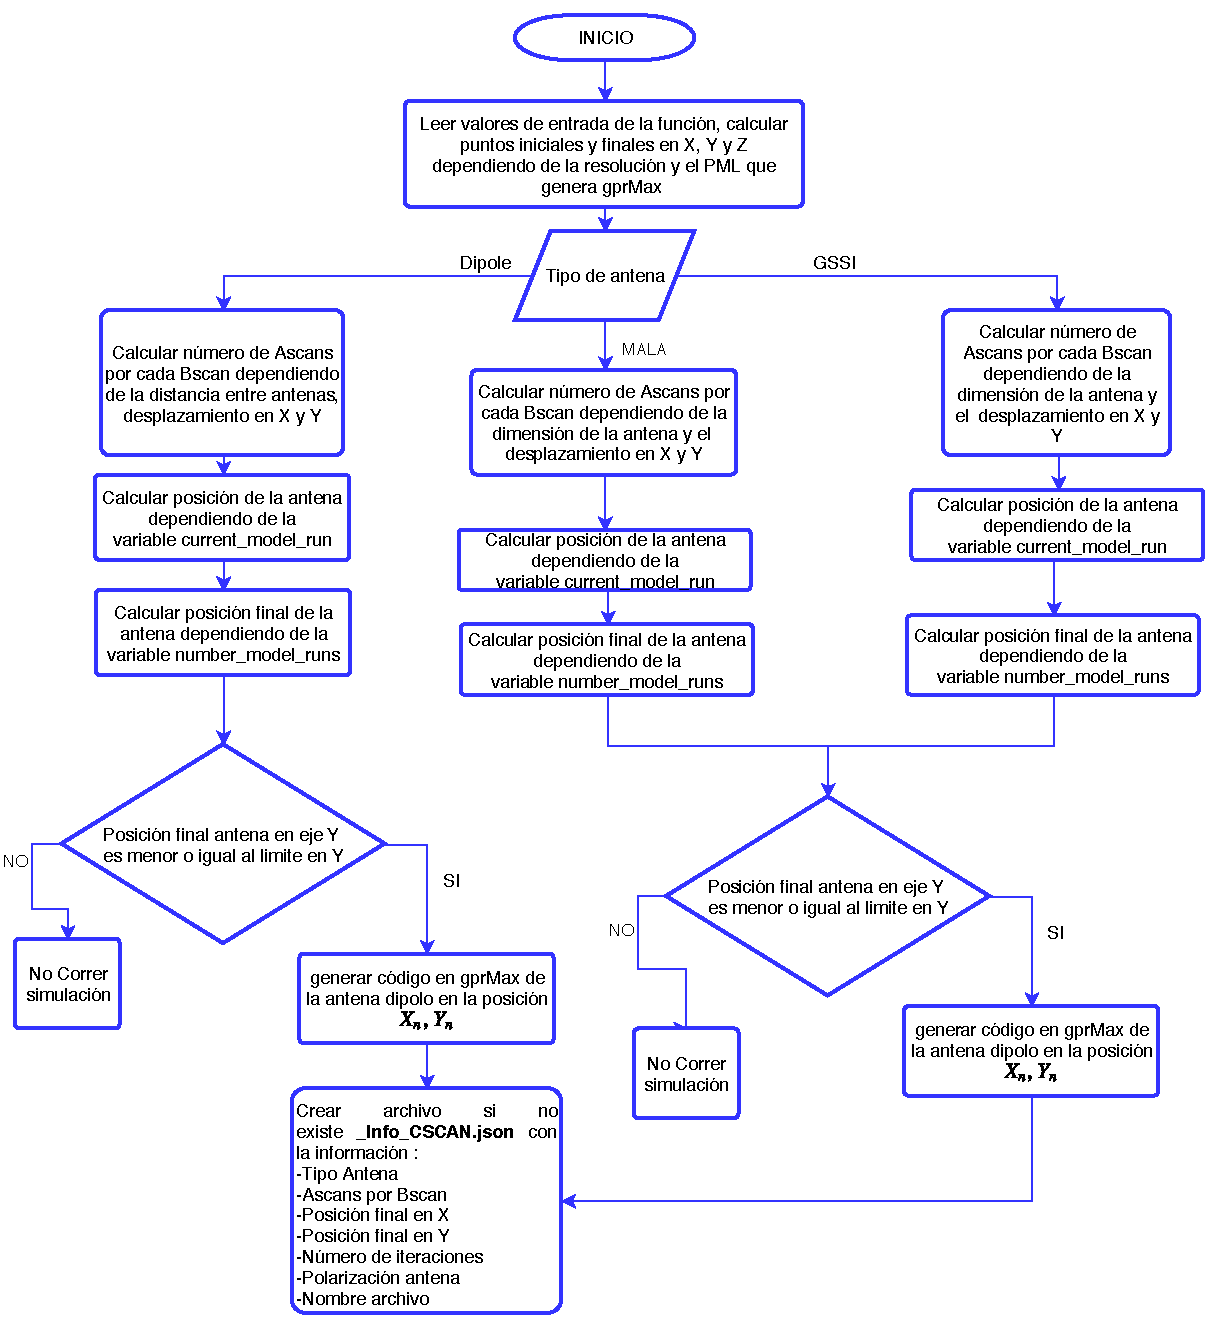
\includegraphics[height=\textheight-9cm,keepaspectratio]{chapter1/images/diagrama_flujo_cscan.pdf}
\caption{Diagrama de flujo generar trazas C}
\label{fig:FlowDiag_TrazasC}
\end{figure}
El resultado del modulo diseñado para generar trazas C en gprMax se puede puede apreciar en la  \figurename{ \ref{img:exampleCscan1GSSI}} donde se muestra los cambios de una antena GSSI realizando mediciones sobre el eje X donde se encuentra una barra metálica enterrada a  5cm de profundidad. El código implementado se encuentra en la sección de anexos como \lstlistingname{ \ref{code:generate_cscan}}. El modulo generará un archivo resultante llamado \textbf{\textit{\_Info\_CSCAN.json}} que contendrá la información del modelo simulado con el modulo implementado porque los resultados del simulador son solo trazas A. Más adelante veremos la estructura de este archivo resultante y como se utiliza para combinar las trazas A.

\begin{figure}[H]  
\centering
\subfigure[Iteración 1 en gprMax ]{
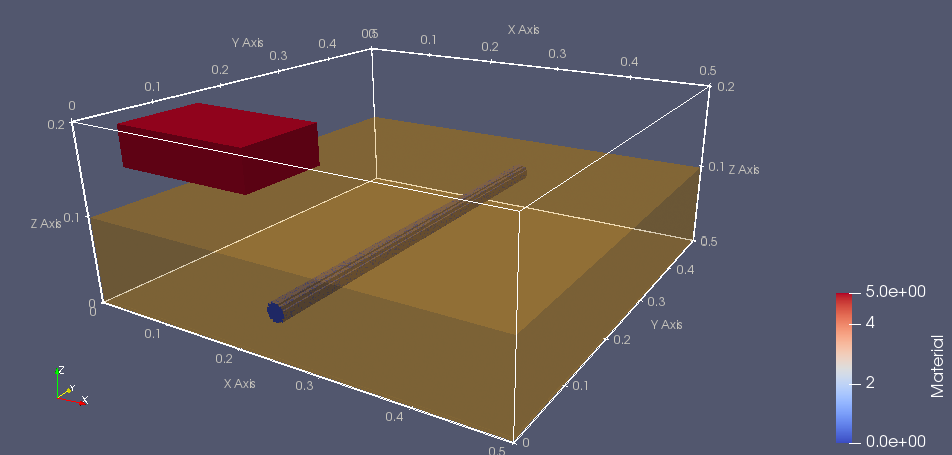
\includegraphics[width=0.3\textwidth, keepaspectratio,valign=c]{chapter1/images/sim_1_GSSI0000.png}
\label{fig:subfig1xampleCscan1GSSI}
}
\subfigure[Iteración 111 en gprMax]{
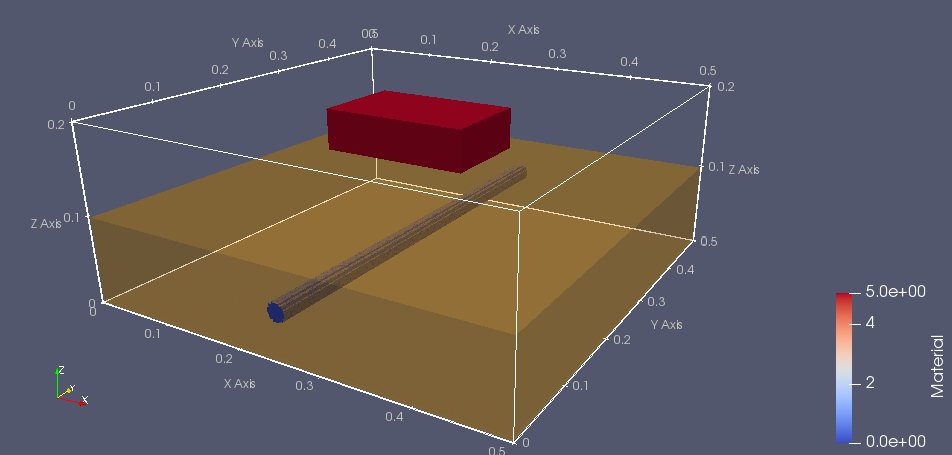
\includegraphics[width=0.3\textwidth, keepaspectratio,valign=c]{chapter1/images/sim_1_GSSI0111.png}
\label{fig:subfig2exampleCscan1GSSI}
}
\subfigure[Iteración 220 en gprMax]{
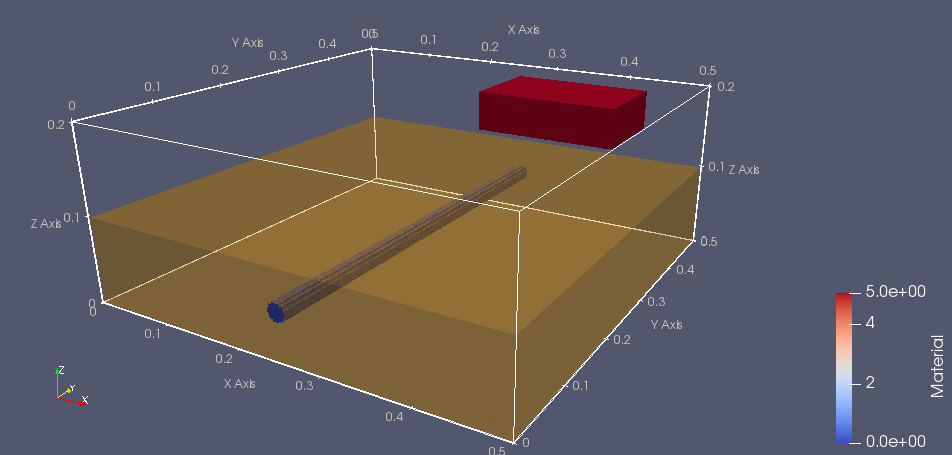
\includegraphics[width=0.3\textwidth, keepaspectratio,valign=c]{chapter1/images/sim_1_GSSI0220.png}
}

\caption{Resultado del desplazamiento de 5cm en cada eje de la antena GSSI para realizar trazas C}
\label{fig:exampleCscan1GSSI}


\end{figure}




%%%%%%%%%%%  SUBSECTION %%%%%%%%%%%%%%%%%% 
\subsection{Calculadora de iteraciones para generar Trazas C}

Para el uso correcto del módulo dentro del simulador es necesario conocer el número de iteraciones requeridas para cubrir todo el dominio en el eje \(x\) y en el eje \(y\) . Se desarrolló un programa en Python que permitiera entregar el resultado de las iteraciones según las condiciones del modelo a simular. En la \figurename{ \ref{fig:FlowDiag_calc_iter}} se encuentra el diagrama de flujo del programa y el \lstlistingname{ \ref{code:calc_iter}} el programa asociado al flujo.


\begin{figure}[H]
\centering
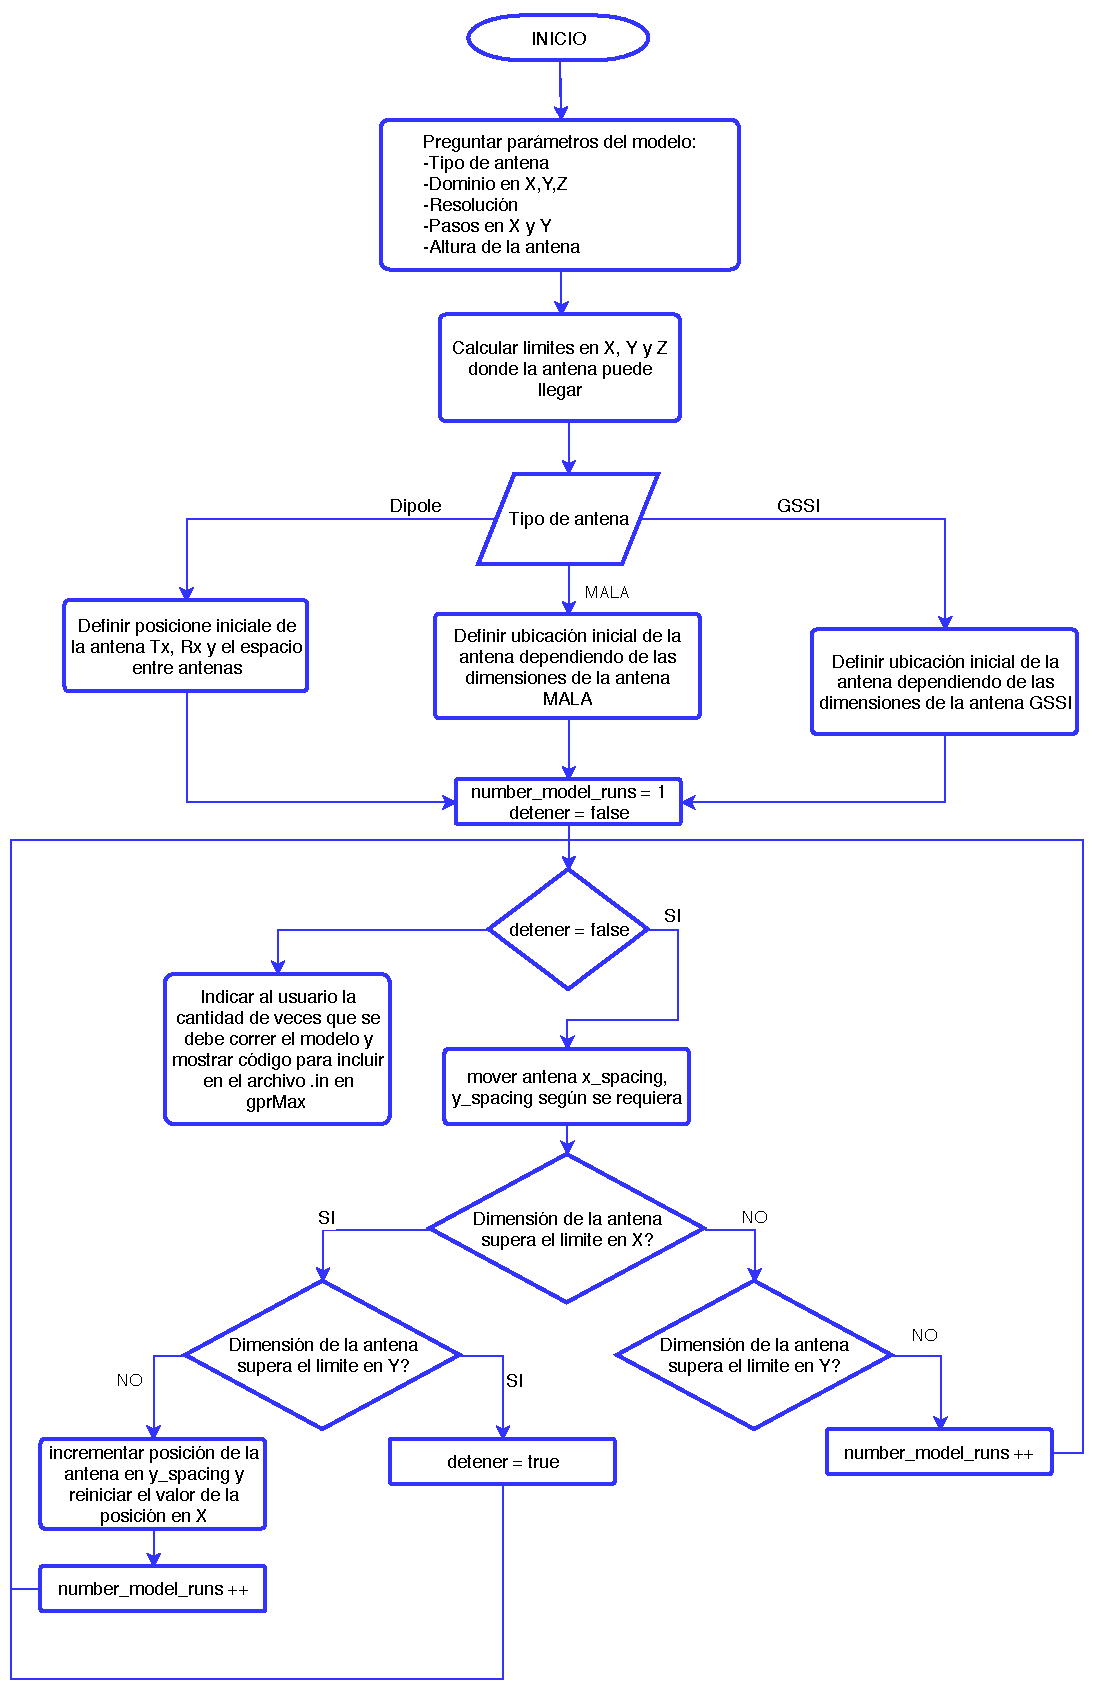
\includegraphics[height=\textheight-4.5cm,keepaspectratio]{chapter1/images/diagrama_flujo_calcular_iteraciones.pdf}
\caption{Diagrama de flujo para calcular el número de iteraciones}
\label{fig:FlowDiag_calc_iter}
\end{figure}

El programa inicia preguntando al  usuario los diferentes parámetros de simulación que van a tener en cuenta cuando se ejecute el modelo en gprMax, la \figurename{ \ref{fig:subfigParametros}} muestra las siete preguntas necesarias para encontrar el numero de iteraciones.  La  \figurename{ \ref{fig:subfigResultados}}  muestra el resultado del algoritmo indicando el numero de iteraciones a colocar en el simulador y en  \ref{fig:subfigResultadosModelo} la integración en un archivo \textbf{\textit{.in}} de gprMax


\begin{figure}[H]   
\centering
\subfigure[Indicando parámetros del modelo]{
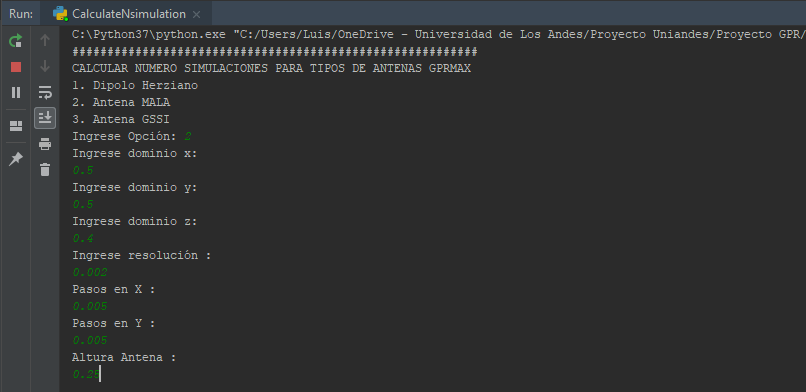
\includegraphics[width=0.7\textwidth, keepaspectratio,valign=c]{chapter1/images/iteraciones1.png}
\label{fig:subfigParametros}
}
\subfigure[Entrega de resultados del algoritmo]{
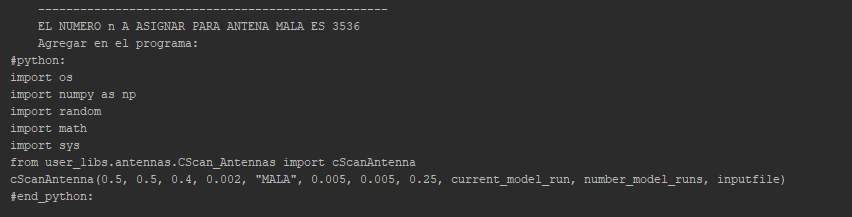
\includegraphics[width=0.7\textwidth, keepaspectratio,valign=c]{chapter1/images/iteraciones2.png}
\label{fig:subfigResultados}
}
\subfigure[Ejemplo en archivo .in gprMax]{
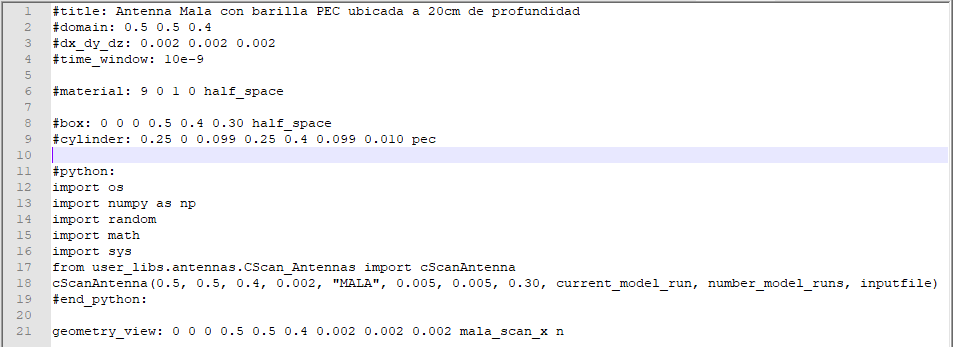
\includegraphics[width=0.7\textwidth, keepaspectratio,valign=c]{chapter1/images/ejemplo_cscan.png}
\label{fig:subfigResultadosModelo}
}

\caption{Funcionamiento algoritmo para calcular iteraciones}
\label{fig:calcularIteraciones}


\end{figure}





%%%%%%%%%%%  SUBSECTION %%%%%%%%%%%%%%%%%% 
\newpage
\subsection{Correr Múltiples Escenarios}

Para optimizar el proceso de simulación de escenarios en la herramienta gprMax, se creo un programa en Python que se encarga de leer archivos de configuración en formato \textbf{\textit{.json}} de tal forma que le permita ejecutar un número prácticamente ilimitado de modelos que contenga una carpeta, la  \figurename{ \ref{fig:flow_config_file}} muestra el diagrama de flujo utilizado en el programa para ejecutar los modelos que estén dentro de una carpeta y el \lstlistingname{ \ref{code:run_muliple}} es el algoritmo utilizado para este diagrama de flujo.

Al momento de realizar las simulaciones en gprMax debe indicarse la ruta y el nombre del archivo \textbf{\textit{.in}}, con el algoritmo desarrollado no es necesario realiza esto. Para ello se debe crear en cada carpeta de simulación un archivo llamado \textbf{\textit{configure\_model.json}}, así como se ve en la \figurename{ \ref{fig:config_file}}.  
 
\begin{figure}[H]
\centering
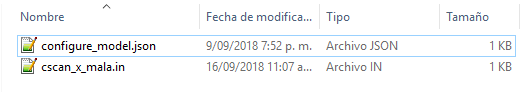
\includegraphics[width=15cm,keepaspectratio]{chapter1/images/archivos_modelo.png}
\caption{Archivo de configuración}
\label{fig:config_file}
\end{figure}

El contenido del archivo \textbf{\textit{configure\_model.json}}  debe tener la siguiente estructura 
\begin{lstlisting} []
{
    "n":2496, 
    "geometry-only":false
}
\end{lstlisting}
donde \textbf{n} corresponde al número de iteraciones que va a tener el modelo y \textbf{geometry-only} corresponde si el modelo a ejecutar solo entregará como resultado la geometría. Este ultimo parámetro es importante porque si el usuario quiere tener los archivos \textbf{\textit{.vti}} para mostrar el escenario en ParaView puede hacerlo cambiando el estado a true

\textcolor{red}{Es importante que el archivo \textbf{\textit{.in }} tenga el mismo nombre de la carpeta, de lo contrario el algoritmo no ejecutará la simulación.}

Cuando se quiera ejecutar el algoritmo es necesario tener otro archivo de configuración, este archivo contendrá las opciones el algoritmo para saber qué carpeta debe revisar y ejecutar todos los modelos que están adentro. A continuación vemos un ejemplo del archivo .json

\begin{lstlisting} []
{
"multiFolder":false,
"directory": "C:\Users\Luis\Desktop\medidas"
}
\end{lstlisting}

Si el usuario no quiere correr todos los modelos de una carpeta puede cambiar el estado de \textit{multifolder} a true, y en ella agregar la opción \textit{models}; esta opción es un arreglo que contiene el nombre de los modelos a ejecutar.

\begin{lstlisting} []
{
"multiFolder":true,
"directory": "C:\Users\Luis\Desktop\medidas",
"models" : ["cscan_x_dipole","cscan_x_gssi"]
}
\end{lstlisting}

Para ejecutar el archivo basta con colocar la siguiente linea de comando \textcolor{blue}{\textbf{python run\_file.py <url archivo .json>}}


\begin{figure}[H]
\centering
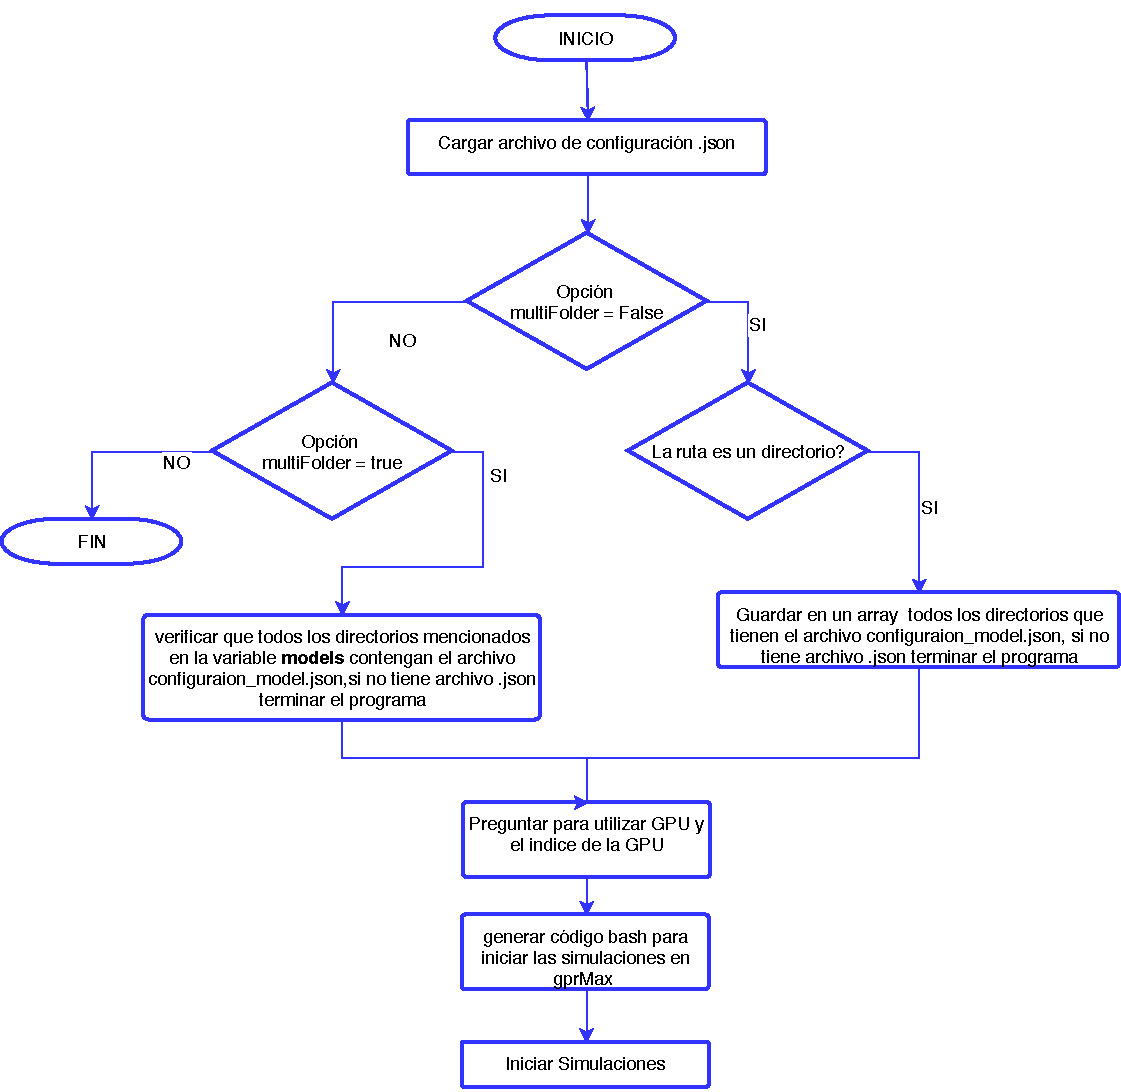
\includegraphics[height=\textheight-3.5cm,keepaspectratio]{chapter1/images/diagrama_flujo_run_multiple.pdf}
\caption{Diagrama de flujo correr múltiples escenarios}
\label{fig:flow_config_file}
\end{figure}


%%%%%%%%%%%  SUBSECTION %%%%%%%%%%%%%%%%%% 
\subsection{Combinar series de Tazas A para generar Trazas B}

Una vez gprMax termina de realizar la simulación de los modelos indicados por el usuario, en las carpetas de los diferentes modelos van a estar los archivos \textbf{\textit{.out}} que corresponden a las trazas A de las diferentes iteraciones realizadas con la librería para genera la traza C; y por otro lado va a contener un archivo de resultados llamado  \textbf{\textit{\_Info\_CSCAN.json}}, el contenido del archivo tendrá información similar a la siguiente:

\begin{lstlisting} []
{
 "antennaType": "GSSI", 
 "scansPerBScan": 52, 
 "finalPositionXEdge": 0.467, 
 "finalPositionYEdge": 0.372,
 "finalAntennaPointX": 0.375, 
 "finalAntennaPointY": 0.3175, 
 "number_model_runs": 2496, 
 "inputfile": "/home/gprmaxtest/gprMax/user_models/luis/cscan/cscan_x_gssi/cscan_x_gssi.in"
 }
\end{lstlisting}

Con esta información se modificó el archivo original \textbf{\textit{outputfiles\_merge.py}} donde deba leer el archivo  de resultados  y saber cuantas trazas A conforman una traza B. En la \figurename{ \ref{fig:merge_traces}} se observa el diagrama de flujo del programa y el \lstlistingname{  \ref{code:merge_multipleAscan}} el algoritmo desarrollado.

Para ejecutar el archivo basta con colocar la siguiente linea de comando \textcolor{blue}{\textbf{python merge\_multiple\_Ascans.py <url archivo .json>}}


Con estos códigos desarrollados en Python es posible inciar las etapas de pre-procesamiento  y migración.

\begin{figure}[H]
\centering
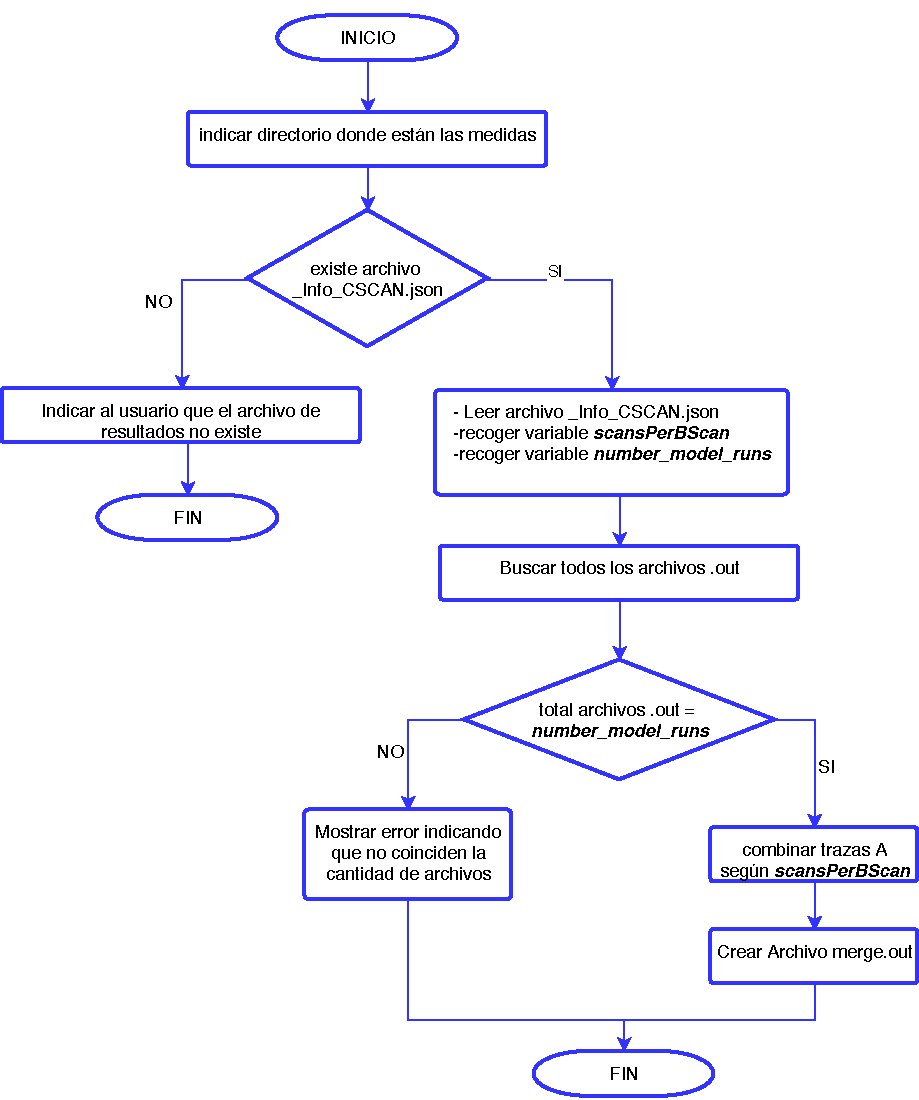
\includegraphics[height=\textheight-3.5cm,keepaspectratio]{chapter1/images/flujo_combinar_trazas.pdf}
\caption{Diagrama de flujo combinar trazas A para crear trazas B}
\label{fig:merge_traces}
\end{figure}



\section{Avance de proyecto especial}

Para el desarrollo del proyecto especial se contemplaron cuatro fases que consisten en:

\begin{itemize}
\item La primera fase corresponde a la consulta de diferentes algoritmos utilizados en el pre-procesamiento de datos en crudo de sistemas GPR, para ello se consultarán libros y artículos en bases de datos científicas
\item La segunda fase consiste en definir el tipo de algoritmo o el conjunto de algoritmos de pre-procesamiento a implementar para el GPR de laboratorio ubicado en la universidad de los Andes, este algoritmo será desarrollado en Matlab o Python.
\item La tercera fase corresponde a la implementación de diferentes pruebas con el GPR de laboratorio; serán ubicados diferentes objetos (metálicos y no metálicos) con el fin de obtener un banco de medidas en crudo para realizar el pre-procesamiento. Es importante que durante esta fase se documente de manera muy detallada las pruebas, porque se busca que las condiciones del laboratorio sean repetitivas para obtener los mismos resultados en cualquier momento
\item La cuarta fase corresponde a la implementación del algoritmo o el conjunto de algoritmos a las diferentes medidas realizadas con el GPR de laboratorio y validar mediante el análisis de resultados el rendimiento del algoritmo
\end{itemize}

\subsection{Calendario Propuesto}

\begin{figure}[H]
\centering
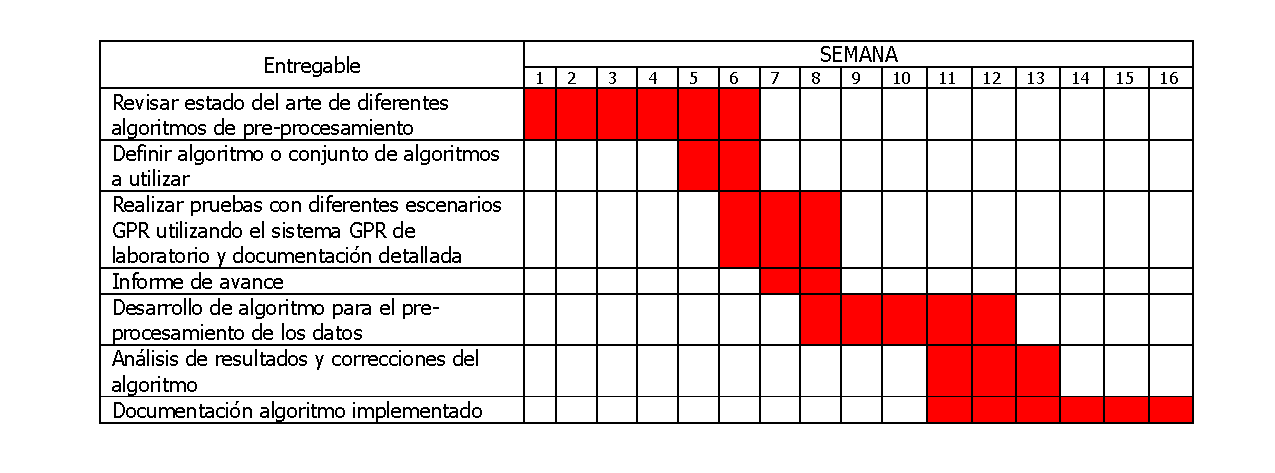
\includegraphics[height=6.5cm,keepaspectratio]{chapter2/images/Calendario_ProyectoEspecial.pdf}

\caption{Cronograma propuesto para Tesis I }
\label{fig:ch1_cronograma_propuesto_tesis}
\end{figure}


De acuerdo al calendario y fases propuestas, al día de la presentación del informe se ha realizado:

\begin{itemize}
\item Revisión del estado del arte de algoritmos de pre-procesamiento en bases de datos científica (IEEE) donde se revisó con el profesor Roberto Bustamante diferentes artículos que permitieran abordar el tema sin tener que recurrir a métodos extremadamente complejos para su desarrollo. 

\item Selección del algoritmo: En el cronograma se destinó la semana 5 y 6 para definir los algoritmos de pre-procesamiento; esta actividad se viene realizando desde el primer día de revisión de los artículos ya que era necesario revisar la implementación del algoritmo en Matlab a medida que se realizaba la lectura.

\item  Implementación de dos algoritmos de pre-procesamiento en las trazas obtenidas mediante simulación ya que se presento un inconveniente de adquisición de datos en medidas de laboratorio.  El VNA necesita estar calibrado,  en el laboratorio se están utilizando cables y antenas con conectores SMA pero el Kit de calibración solo es tipo N; se realizó la solicitud de cotización a la empresa Metricom del kit de calibración SMA, pero mientras se realiza esta compra se tomó la  decisión de utilizar datos simulados.

\item Simulaciones de diferentes modelos con objetos para aplicar los algoritmos de pre-procesamiento, estos resultados se encuentran más adelante. 

\end{itemize}




\subsection{Estado del arte}
Para la revisión del estado del arte inicialmente se realizó la lectura del capitulo 5 del libro \textit{Ground penetrating radar theory and applications} \cite{gpr_HarryM} donde contempla la etapa de procesamiento de datos GPR crudos (raw data) para eliminar el ruido que se presenta en cada una de las trazas proveniente de diferentes elementos presentes en un suelo, como lo es: el acople mutuo entre antenas (producido por la señal que llega directamente a la antena transmisora de la antena receptora), Las primeras reflexiones causadas por la interfaz aire-suelo, y las reflexiones causadas por elementos están enterrados bajo tierra y que pueden llegar a generar falsas alarmas. 

En este documento se presentan diferentes etapas de procesamiento tales como: interpolación del ``ruber-band''; filtro Dewow para eliminar componentes de frecuencia baja; Time-zero correction para corregir y ajustar un tiempo ``zero'' donde ocurre la primera reflexión en todas las trazas; filtrado; deconvolución; funciones de ganancia y migración.

En la universidad Louvain-la-Neuve (Belgica) , el instituto de tierra \cite{Detection_of_Reflection_Hyperbolas} desarrolló un método de detección de hipérbolas mediante filtros  donde la etapa de pre-procesamiento era importante para eliminar características constantes de que se presentaban en las trazas y luego llevar a cabo la detección de hiperboas mediante filtros Canny.

Raffaele Solimene et al. \cite{Ground_Clutter_Removal_in_GPR_Surveys} muestra como las reflexiones producidas por los suelos pueden impedir la detección de objetos enterrados debido a la magnitud de la señal y las frecuencias del sistema GPR, este tipo de ruido puede ser mitigado mediante la aplicación de algoritmos  basados en la entropía de los datos. En este documento se implementan dos etapas de pre-procesamiento, el ``Mean Substraction'' y el ``subspace projection'' para aplicar el método de entropía en la detección de ub objeto metalico de 26cm de largo y teniendo una sección trasversal de 4cm x 3cm enterrados a una distancia de 4cm; Utilizan un kit de radar (Ris-K2) que trabaja a una frecuencia de 2GHz, los resultados muestran que la aplicación de los algoritmos ``Mean Substraction'' y  ``subspace projection''  entregan resultados muy similares  y aplicando el metodo de entropia, supera el resultado de los dos algoritmos.

En la universidad nacional de defensa tecnológica Changsha, china \cite{Improving_RPCA-Based_Clutter_Suppression} implementaron un método novedoso para eliminar el ruido de los datos GPR en la detección de minas antipersonales basado en el algoritmo  ``Robust principal component analysis'' (RPCA). El algoritmo se encarga de separar las señales de ruido (Low-Rank) de la señales de los objetos (Sparse). Una vez implementado el algoritmo les permitió utilizar algoritmos de migración en las señales de los objetos (Sparse). Su trabajo concluye en que la combinación del algoritmo RPCA con el de migración es óptimo para separar las señales en ambientes con mucho clutter debido a su robustes.

Priyadarshini et al. \cite{Buried-Discrimination-gpr-Radar-Radargram} implementa un método para discriminar las señales clutter de los objetos en las señales GPR aplicando dos etapas de pre procesamiento y un análisis espectral para determinar si el objeto si es una mina.

En la etapa de pre-procesamiento utiliza el algoritmo ``Ensamble Averaging''  que es el mismo ``Mean Substraction'' de los otros articulos encontrados. Una vez aplica dicho algoritmo, implementa un algoritmo en cascada llamado ``Entropy Optimized Contrast Stretching'' mediante los algoritmos  ``Contrast Stretching'' (CS) y ``Entropy Optimized'' para hacer un mejor uso del rango dinámico de la imagen y de esta manera se pueda apreciar mejor las hipérbolas en las trazas B.

Como resultado de dicho trabajo es la eliminación del clutter y mejorando la imagen de la traza B para poder discriminar objetos de diferentes tamaños, con dichos resultados, le permitió aplicar algoritmos métodos de detección mediante técnicas de análisis espectral.

Por último Anonios Giannopolus et al. crean un modelo basado en inteligencia artificial mediante redes neuronales  para entrenar un algoritmo que sea capaz de reconocer las señales provenientes de un ojeto y discriminar las señales de ruido en tiempo real \cite{gprMax,Evaluation_of_Signal-to-Clutter_Ratio}

\subsection{Algoritmos Implementados}

De acuerdo con la revisión del estado del arte y de acuerdo a los resultados obtenidos se ha decidido utilizar algunos de los algoritmos mencionados, por ejemplo, el algoritmo utilizado en \cite{Improving_RPCA-Based_Clutter_Suppression} demuestra una gran utilidad para separar el ruido de la señal de la mina (target) u otro objeto a sin conocer las condiciones del suelo, lo que es de gran utilidad al momento de usar un sistema GPR.

Por otro lado se utilizó también el algoritmo ``Mean Substraction'' ya que a pesar que es uno de los algoritmos mas sencillos, es utilizado lo la mayoría de los artículos. A continuación se mostrará el desarrollo de cada uno de los algoritmos en las señales de los modelos simulados.
\subsubsection{Robust PCA}
Robust Principal Component Analysis es un algoritmo  desarrollado en conjunto por la universidad de Illinois y  Standford \cite{Candes:RPCA} que fue utilizado inicialmente en aplicaciones de visión por computador. En la actualidad uno de los problemas al analizar datos es poder extraer información intrínseca de un conjunto de datos. 

\begin{figure}[H]
\centering
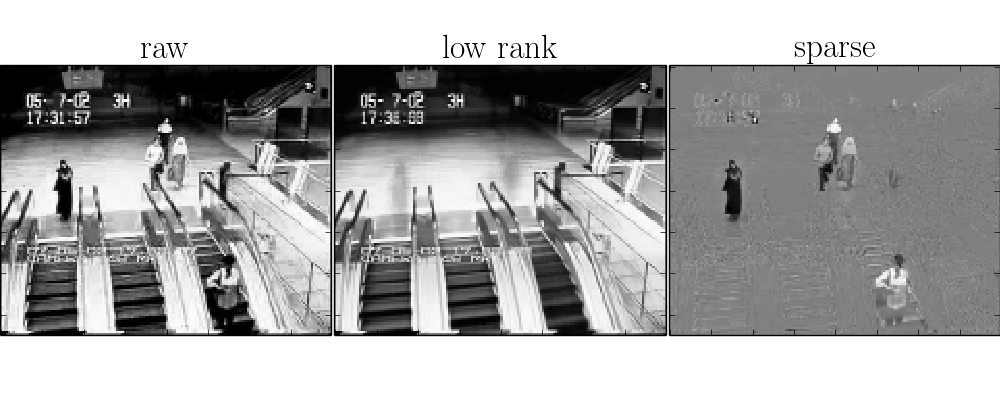
\includegraphics[height=6.5cm,keepaspectratio]{chapter2/images/example_RPCA.png}

\caption{Ejemplo RPCA en aplicaciones de vídeo }
\label{fig:example_rpca}
\end{figure}

El uso de este algoritmo es de gran importancia en las aplicaciones de GPR para eliminar clutter sin conocer las propiedades del suelo que esta bajo medición.

Matemáticamente, RPCA puede ser observada como una matriz D de la siguiente forma:

\begin{equation}
    D=L+S+N
    \label{eq:rpca_general}
\end{equation}

Donde \textbf{L} indica la matriz Low-Rank o Background que representa todas las señales de fondo, para GPR estas señales pueden ser las múltiples reflexiones en la interfaz aire-suelo y el acople entre antenas; \textbf{S} la matriz Sparse son los objetos en primer plano  que correspoderían a todas las señales propias de las minas (target)   y \textbf{N} un termino de ruido. En \cite{rpca_review}  no se tiene en cuenta ya que se puede ver \textbf{L} y \textbf{N} como un solo valor.

Las secuencias que se presentan en el fondo puede ser modeladas como un sub espacio que cambia gradualmente con respecto al tiempo (Matriz \textbf{L}), mientras que los objetos en movimiento constituyen eventos atípicos que pueden ser correlacionados.


La matriz D se puede descomponer como el siguiete problema de optimización:
\begin{equation}
\min _{ L,S }{ { \left\| L \right\|  }_{ * } } +\lambda {\left\| S \right\| }_{1}\quad \quad  con \quad   restricción\quad  D-L-S=0
\label{eq:minimizar}
\end{equation}


Donde  la norma ${ \left\|  \bullet \right\|  }$ (nuclear norm) corresponde a la la suma de los valores singulares de la matriz L y ${ \left\|  \bullet  \right\|  }_{1}$ es la norma $l^1$ de una matriz vista como vector, este valor es calculado como la suma de los valores absolutos de la matriz D.  $\lambda $  corresponde a un multiplicador lagrangiano 

\subsubsubsection{\textbf{Implementación RPCA en trazas gprMax}}

Se desarrolló en Matlab un algoritmo que permitiera seleccionar una cantidad N de trazas B para aplicarle a cada componente de campo (Ex,Ey,Ez,Hx,Hy,Hz) el algoritmo RPCA, el código implementado es el siguiente:

\begin{lstlisting}[ basicstyle=\tiny]
% get_RPCA_Bscans.m
% Los Andes University
% Creaded By: Luis Eduardo Quibano Alarcon
% E-mail: le.quibano@uniandes.edu.co
% Description: This Script  opens a specific amoun of  Bscans in order to
%              apply them the RPCA algotrithm in all field  components of
%              each A-scan, The result of this algorithm gives L and S
%              matrixes; create a new set of B_scans of the resulting
%              matrixes L and S
% RPCA algoithm : https://statweb.stanford.edu/~candes/papers/RobustPCA.pdf
% Original Github Repository: https://github.com/dlaptev/RobustPCA

clear all
close all
clc

[filename, pathname] = uigetfile('*.out', 'Select gprMax B-scans output files','MultiSelect','on');
fullfilename = strcat(pathname, filename);

filename = cellstr(filename);
pathname = cellstr(pathname);
fullfilename = cellstr(fullfilename);

%Extraigo todos los campos de los A-scan seleccionados y luego los guardo
%en la matriz del objeto fields{i}
if length(fullfilename) ~=0
    for i=1:length(fullfilename)
        if filename{i} ~= 0
            iterations = double(h5readatt(fullfilename{i}, '/', 'Iterations'));
            dt = h5readatt(fullfilename{i}, '/', 'dt');
            
            ExFieldPath = strcat('/rxs/rx1/', 'Ex');
            EyFieldPath = strcat('/rxs/rx1/', 'Ey');
            EzFieldPath = strcat('/rxs/rx1/', 'Ez');
            HxFieldPath = strcat('/rxs/rx1/', 'Hx');
            HyFieldPath = strcat('/rxs/rx1/', 'Hy');
            HzFieldPath = strcat('/rxs/rx1/', 'Hz');
            
            
            ExAllScans = h5read(fullfilename{i}, ExFieldPath);
            EyAllScans = h5read(fullfilename{i}, EyFieldPath);
            EzAllScans = h5read(fullfilename{i}, EzFieldPath);
            HxAllScans = h5read(fullfilename{i}, HxFieldPath);
            HyAllScans = h5read(fullfilename{i}, HyFieldPath);
            HzAllScans = h5read(fullfilename{i}, HzFieldPath);
            
            %% APPLY RPCA
            [L_ExAllScans,S_ExAllScans] = getRPCAinComponent('ex',ExAllScans);
            [L_EyAllScans,S_EyAllScans] = getRPCAinComponent('ey',EyAllScans);
            [L_EzAllScans,S_EzAllScans] = getRPCAinComponent('ez',EzAllScans);
            [L_HxAllScans,S_HxAllScans] = getRPCAinComponent('hx',HxAllScans);
            [L_HyAllScans,S_HyAllScans] = getRPCAinComponent('hy',HyAllScans);
            [L_HzAllScans,S_HzAllScans] = getRPCAinComponent('hz',HzAllScans);
            
            %% Create New A-scan set with LowRank And Spare Results
            %Como ya tengo los resultados del algoritmo (L y S) creo los mismos
            %creo los mismos archivos
            generate_LowRank
            generate_Sparse
        end
    end
    
end

%% Funcion del algoritmo RPCA
function [L,S] = getRPCAinComponent(component,data)
%Los datos deben trabajarse de forma normalizada para ello se realiza el
%proceso de encontrar el mayor valor y el menor valor
minVal = min(min(data));
maxVal = max(max(data));
X_norm = (data - minVal) / ( maxVal - minVal );
%Aplicar RPCA
lambda = 1/sqrt(max(size(X_norm)));
tic
[L_norm,S_norm] = RobustPCA(component,X_norm, (lambda/3)*1.5 , ((10*lambda)/3)*1.5, 1e-5,1000);
toc %Me indica el tiempo que tardo en realizar RPCA a los datos de entrada con mil iteraciones
%El resultado del alogoritmo me entrega los de la matriz L y S de forma
%normalizada, para ello, encuentro el valor real.
%los datos de L y S se devuelven en la funcion y son los que se van a
%graficar
L=L_norm.*( maxVal - minVal ) + minVal;
S=S_norm.*( maxVal - minVal ) + minVal;
end
\end{lstlisting}

Como se puede observar se utiliza la función \textit{getRPCAinComponen()} donde su parámetro de entrada son los valores de campo. Más adelante se puede observar que antes de aplicar el algoritmo como tal, los datos necesitan ser normalizados, esta es una condición especial del algoritmo,  así mismo es necesario indicar el valor de $\lambda $, si este valor no es puesto como parámetro, este tomara el valor por defecto de $ 1 / sqrt(max(M,N)$. Una vez los datos se encuentran normalizados los datos entran a la función \textit{RobustPCA()}, esta función entrega como resultados los valores de las matrices $L$ y $S$ normalizadas, estas dos matrices se desnormalizan para obtener los valores originales de campo.


\begin{lstlisting}[ basicstyle=\tiny]
function [L, S] = RobustPCA(component,X, lambda, mu, tol, max_iter)
    % - component is the string of the name of the component which is
    % applied RPCA
    % - X is a data matrix (of the size N x M) to be decomposed
    %   X can also contain NaN's for unobserved values
    % - lambda - regularization parameter, default = 1/sqrt(max(N,M))
    % - mu - the augmented lagrangian parameter, default = 10*lambda
    % - tol - reconstruction error tolerance, default = 1e-6
    % - max_iter - maximum number of iterations, default = 1000

    [M, N] = size(X);
    unobserved = isnan(X);
    X(unobserved) = 0;
    normX = norm(X, 'fro');

    % default arguments
    if nargin < 2
        lambda = 1 / sqrt(max(M,N));
    end
    if nargin < 3
        mu = 10*lambda;
    end
    if nargin < 4
        tol = 1e-6;
    end
    if nargin < 5
        max_iter = 1000;
    end
    
    % initial solution
    L = zeros(M, N);
    S = zeros(M, N);
    Y = zeros(M, N);
    
    for iter = (1:max_iter)
        % ADMM step: update L and S
        L = Do(1/mu, X - S + (1/mu)*Y);
        S = So(lambda/mu, X - L + (1/mu)*Y);
        % and augmented lagrangian multiplier
        Z = X - L - S;
        Z(unobserved) = 0; % skip missing values
        Y = Y + mu*Z;
        
        err = norm(Z, 'fro') / normX;
        if (iter == 1) || (mod(iter, 10) == 0) || (err < tol)
            fprintf(1, 'component: %s   iter: %04d\terr: %f\trank(L): %d\tcard(S): %d\n', ...
                    component,iter, err, rank(L), nnz(S(~unobserved)));
        end
        if (err < tol) break; end
    end
end
function r = So(tau, X)
    % shrinkage operator
    r = sign(X) .* max(abs(X) - tau, 0);
end
function r = Do(tau, X)
    % shrinkage operator for singular values
    [U, S, V] = svd(X, 'econ');
    r = U*So(tau, S)*V';
end
\end{lstlisting}

En la siguientes lineas de códigos se encargan de tomar los datos de la matriz L y crear una nueva traza B y guardarlo en una nueva carpeta de mediciones.

\begin{lstlisting}[ basicstyle=\tiny]

% clear all, clc
% close all
% load('matlab.mat')
fullfilenameLowRank = fullfilename{i};
filenameLowRank=filename{i};
%%CREATE A COPY OF B-SCAN WITH NAME LOW RANK
%%SI LA ITERACION ES LA 1, borrar todas las carpetas y empezar a crear los
%%archivos
if i==1
    if exist(strcat(pathname{1},'/lowrank_bscan')) == 7
        rmdir(strcat(pathname{1},'/lowrank_bscan'), 's')
    end
    mkdir(strcat(pathname{1},'/lowrank_bscan'))
end
pathToSave=strcat(pathname{1},'/lowrank_bscan')


nameSplit = split(filenameLowRank,'.');
nameSplit= nameSplit(1);
nameSplit= strcat(pathToSave,'/',nameSplit{1});
nameSplit=strcat(nameSplit(1:end),'_LowRank','.out');
fullfilenameLowRank=nameSplit ;
copyfile(fullfilename{i}, nameSplit);



%%Modify All LowRank Files

iterations = double(h5readatt(fullfilenameLowRank, '/', 'Iterations'));
dt = h5readatt(fullfilenameLowRank, '/', 'dt');

ExFieldPath = strcat('/rxs/rx1/', 'Ex');
EyFieldPath = strcat('/rxs/rx1/', 'Ey');
EzFieldPath = strcat('/rxs/rx1/', 'Ez');
HxFieldPath = strcat('/rxs/rx1/', 'Hx');
HyFieldPath = strcat('/rxs/rx1/', 'Hy');
HzFieldPath = strcat('/rxs/rx1/', 'Hz');

h5write(fullfilenameLowRank, ExFieldPath,L_ExAllScans);
h5write(fullfilenameLowRank, EyFieldPath,L_EyAllScans);
h5write(fullfilenameLowRank, EzFieldPath,L_EzAllScans);
h5write(fullfilenameLowRank, HxFieldPath,L_HxAllScans);
h5write(fullfilenameLowRank, HyFieldPath,L_HyAllScans);
h5write(fullfilenameLowRank, HzFieldPath,L_HzAllScans);
\end{lstlisting}

De la misma manera ocurre para guardar las trazas B de la matriz S.

\begin{lstlisting}[ basicstyle=\tiny]
%
% clear all, clc
% close all
% load('matlab.mat')
fullfilenameSparse = fullfilename{i};
filenameSparse=filename{i};
%%CREATE A COPY OF B-SCAN WITH NAME LOW RANK
%%SI LA ITERACION ES LA 1, borrar todas las carpetas y empezar a crear los
%%archivos
if i==1
    if exist(strcat(pathname{1},'/sparse_bscan')) == 7
        rmdir(strcat(pathname{1},'/sparse_bscan'), 's')
    end
    mkdir(strcat(pathname{1},'/sparse_bscan'))
end
pathToSave=strcat(pathname{1},'/sparse_bscan')
nameSplit = split(filenameSparse,'.');
nameSplit= nameSplit(1);
nameSplit= strcat(pathToSave,'/',nameSplit{1});
nameSplit=strcat(nameSplit(1:end),'_Sparse','.out');
fullfilenameSparse=nameSplit ;
copyfile(fullfilename{i}, nameSplit);
%%Modify All LowRank Files
iterations = double(h5readatt(fullfilenameSparse, '/', 'Iterations'));
dt = h5readatt(fullfilenameSparse, '/', 'dt');
ExFieldPath = strcat('/rxs/rx1/', 'Ex');
EyFieldPath = strcat('/rxs/rx1/', 'Ey');
EzFieldPath = strcat('/rxs/rx1/', 'Ez');
HxFieldPath = strcat('/rxs/rx1/', 'Hx');
HyFieldPath = strcat('/rxs/rx1/', 'Hy');
HzFieldPath = strcat('/rxs/rx1/', 'Hz');
h5write(fullfilenameSparse, ExFieldPath,S_ExAllScans);
h5write(fullfilenameSparse, EyFieldPath,S_EyAllScans);
h5write(fullfilenameSparse, EzFieldPath,S_EzAllScans);
h5write(fullfilenameSparse, HxFieldPath,S_HxAllScans);
h5write(fullfilenameSparse, HyFieldPath,S_HyAllScans);
h5write(fullfilenameSparse, HzFieldPath,S_HzAllScans);

\end{lstlisting}

En la \figurename{ \ref{fig:results_rpca_folders}} se muestra como se organizan los resultados una vez aplicado el algoritmo RPCA sobre las trazas B, el programa en Matlab se encarga de crear una carpeta llamada \textbf{lowrank\_bcscan} y otra llamada \textbf{sparse\_bscan}
\begin{figure}[H]
\centering
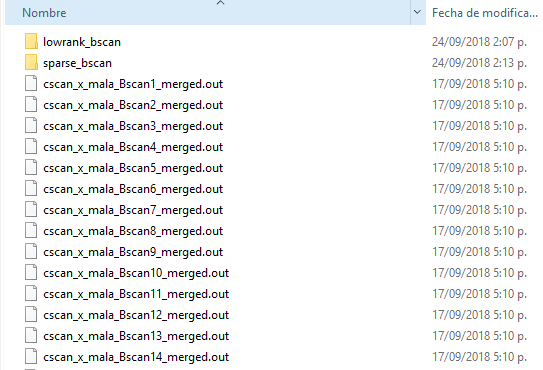
\includegraphics[height=5.5cm,keepaspectratio]{chapter2/images/resultado_rpca_trazasB.png}
\caption{Carpeta de resultados después de aplicar RPCA a las trazas B originales }
\label{fig:results_rpca_folders}
\end{figure}


A continuación se muestra el resultado de aplicar RPCA sobre un modelo de 0.5mx0.5mx0.4m de dominio, con resolución de 0.002m, se utiliza una antena MALA y de desplaza 0.005m en cada iteración.

Se Aplica RPCA a cada componente, pero vamos a observar la señal sobre Ez. En la \figurename{ \ref{fig:bscanRPCA_SIM1}} se observa el resultado del modelo, la traza B original,  y los resultados de extraer el ruido de fondo y la señal de las barras metálicas.



\begin{figure}[H]  
\centering
\subfigure[ Modelo Original ]{
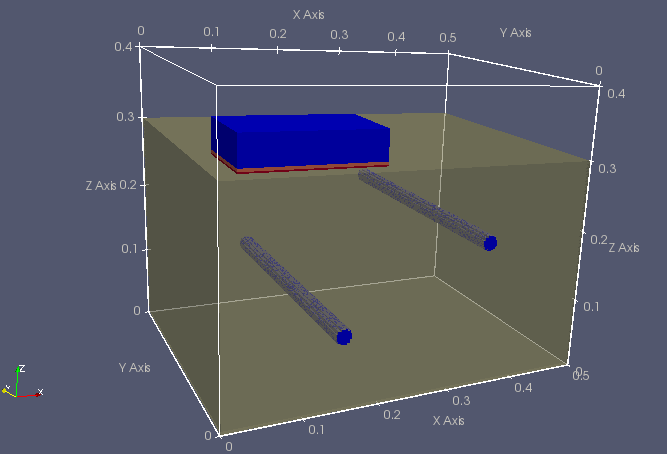
\includegraphics[width=0.35\textwidth, keepaspectratio,valign=c]{chapter2/images/mala_2_barras.png}
\label{fig:subfig_mala2_barras_mod}
}
\subfigure[ Bscan datos crudos ]{
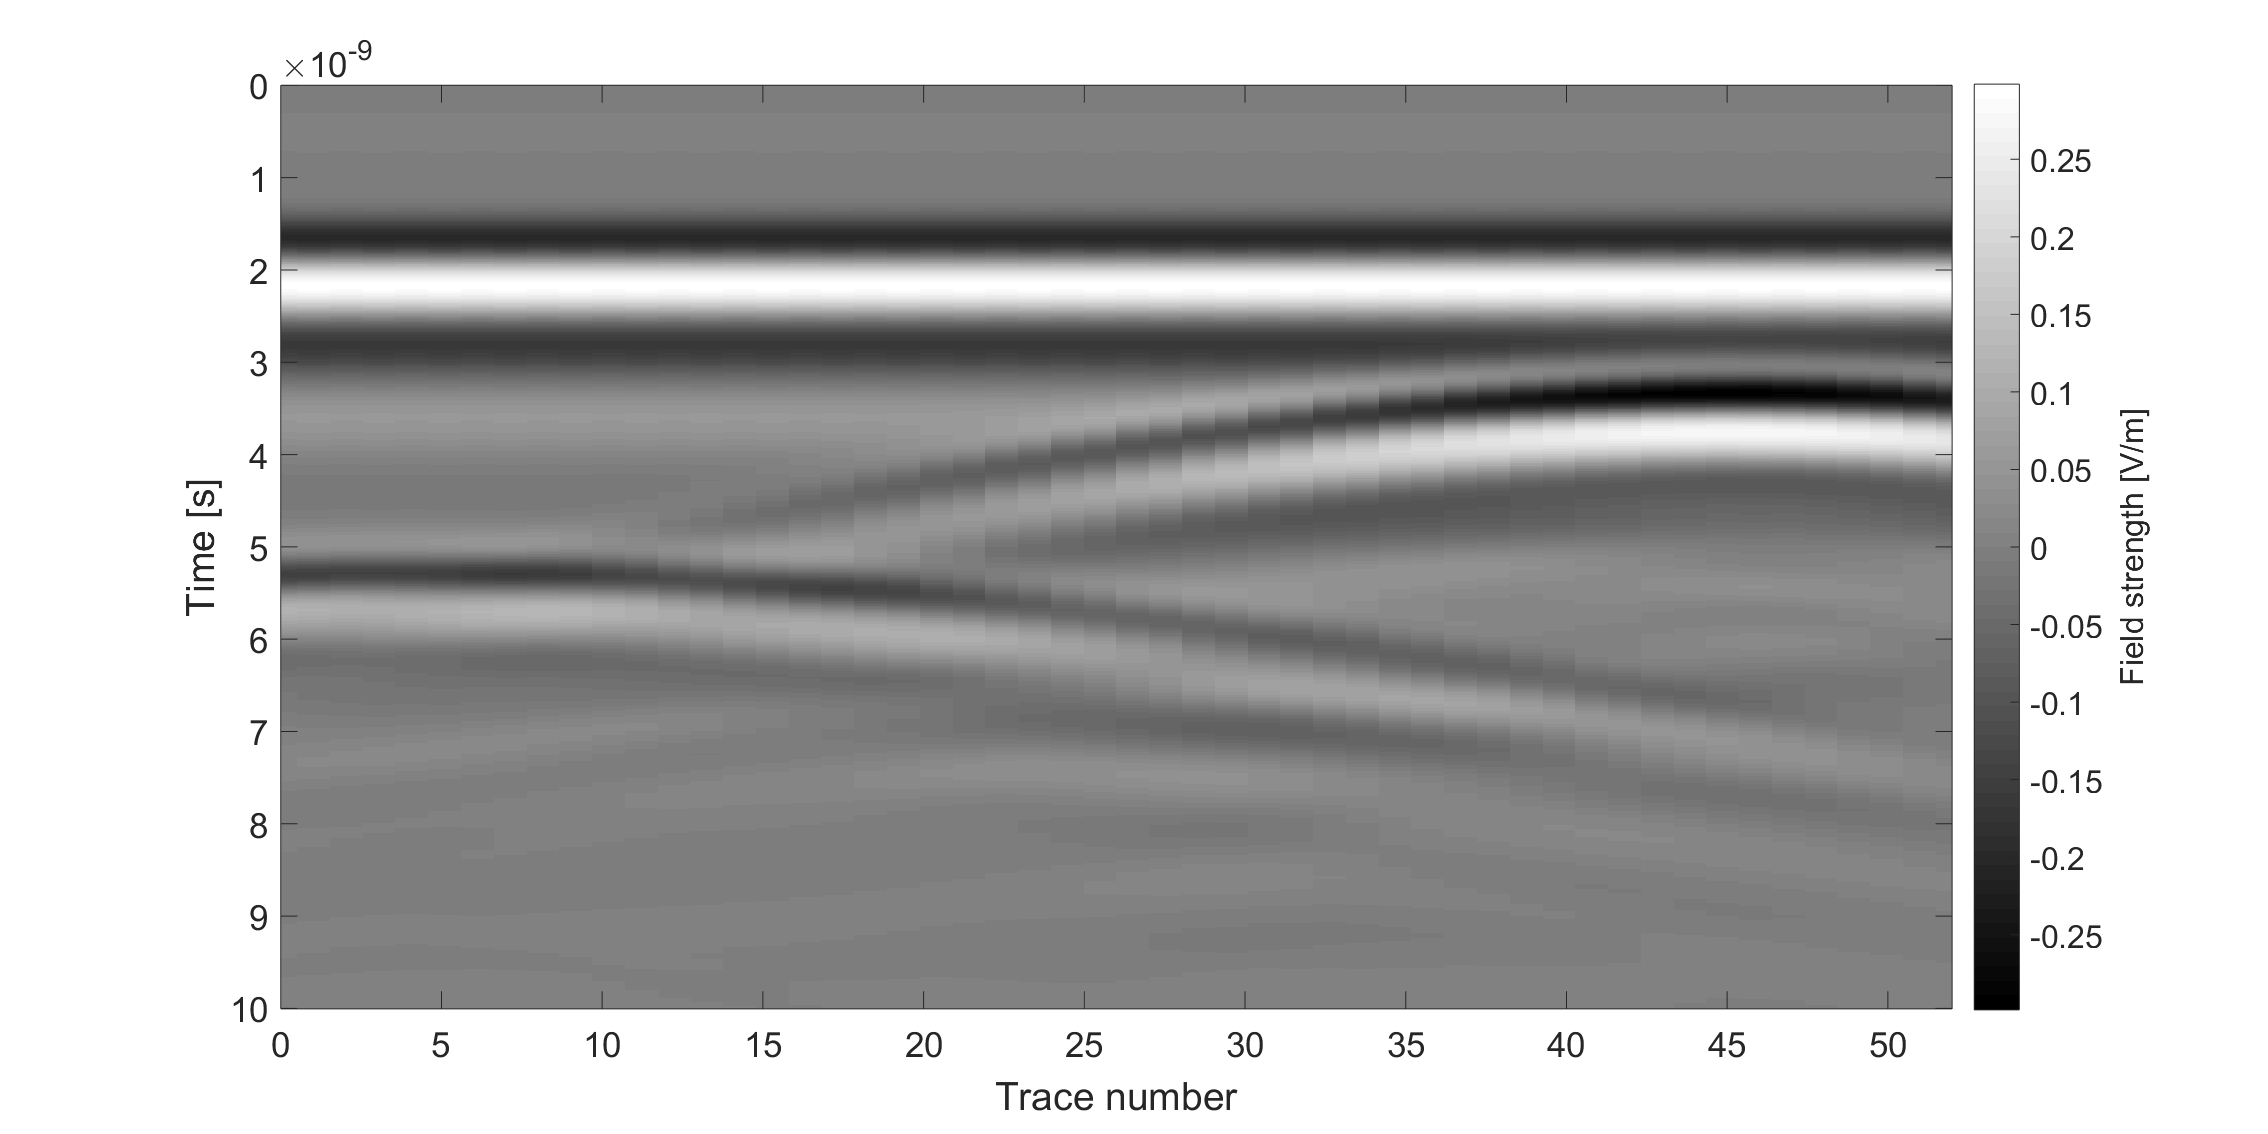
\includegraphics[width=0.55\textwidth, keepaspectratio,valign=c]{chapter2/images/mala_2_barras_bscan.png}
\label{fig:subfig1xampleCscan1GSSI}
} \\
\subfigure[ Bscan Low Rank ]{
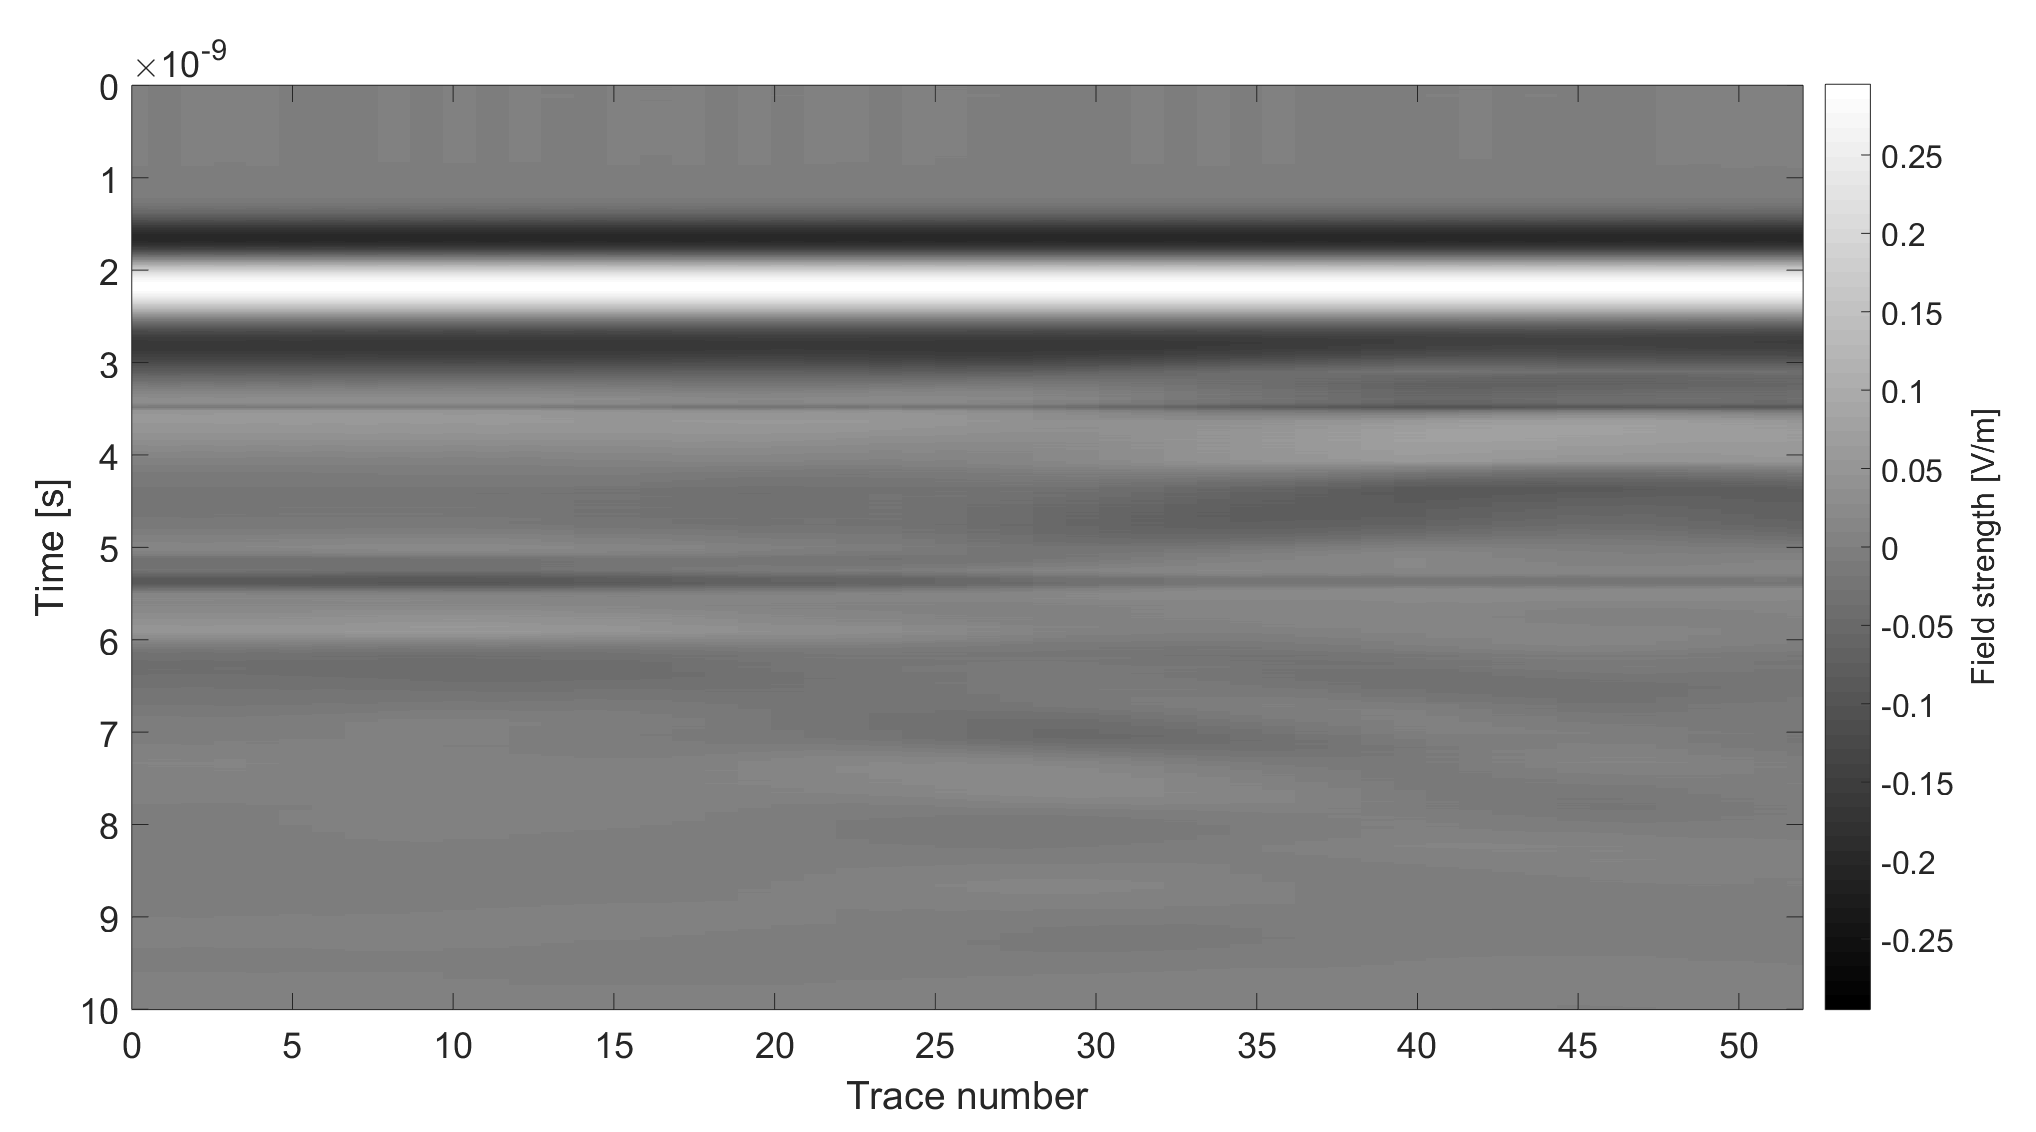
\includegraphics[width=0.47\textwidth, keepaspectratio,valign=c]{chapter2/images/mala_2_barras_bscan_low.png}
\label{fig:subfig2exampleCscan1GSSI}
}
\subfigure[Bscan Sparse ]{
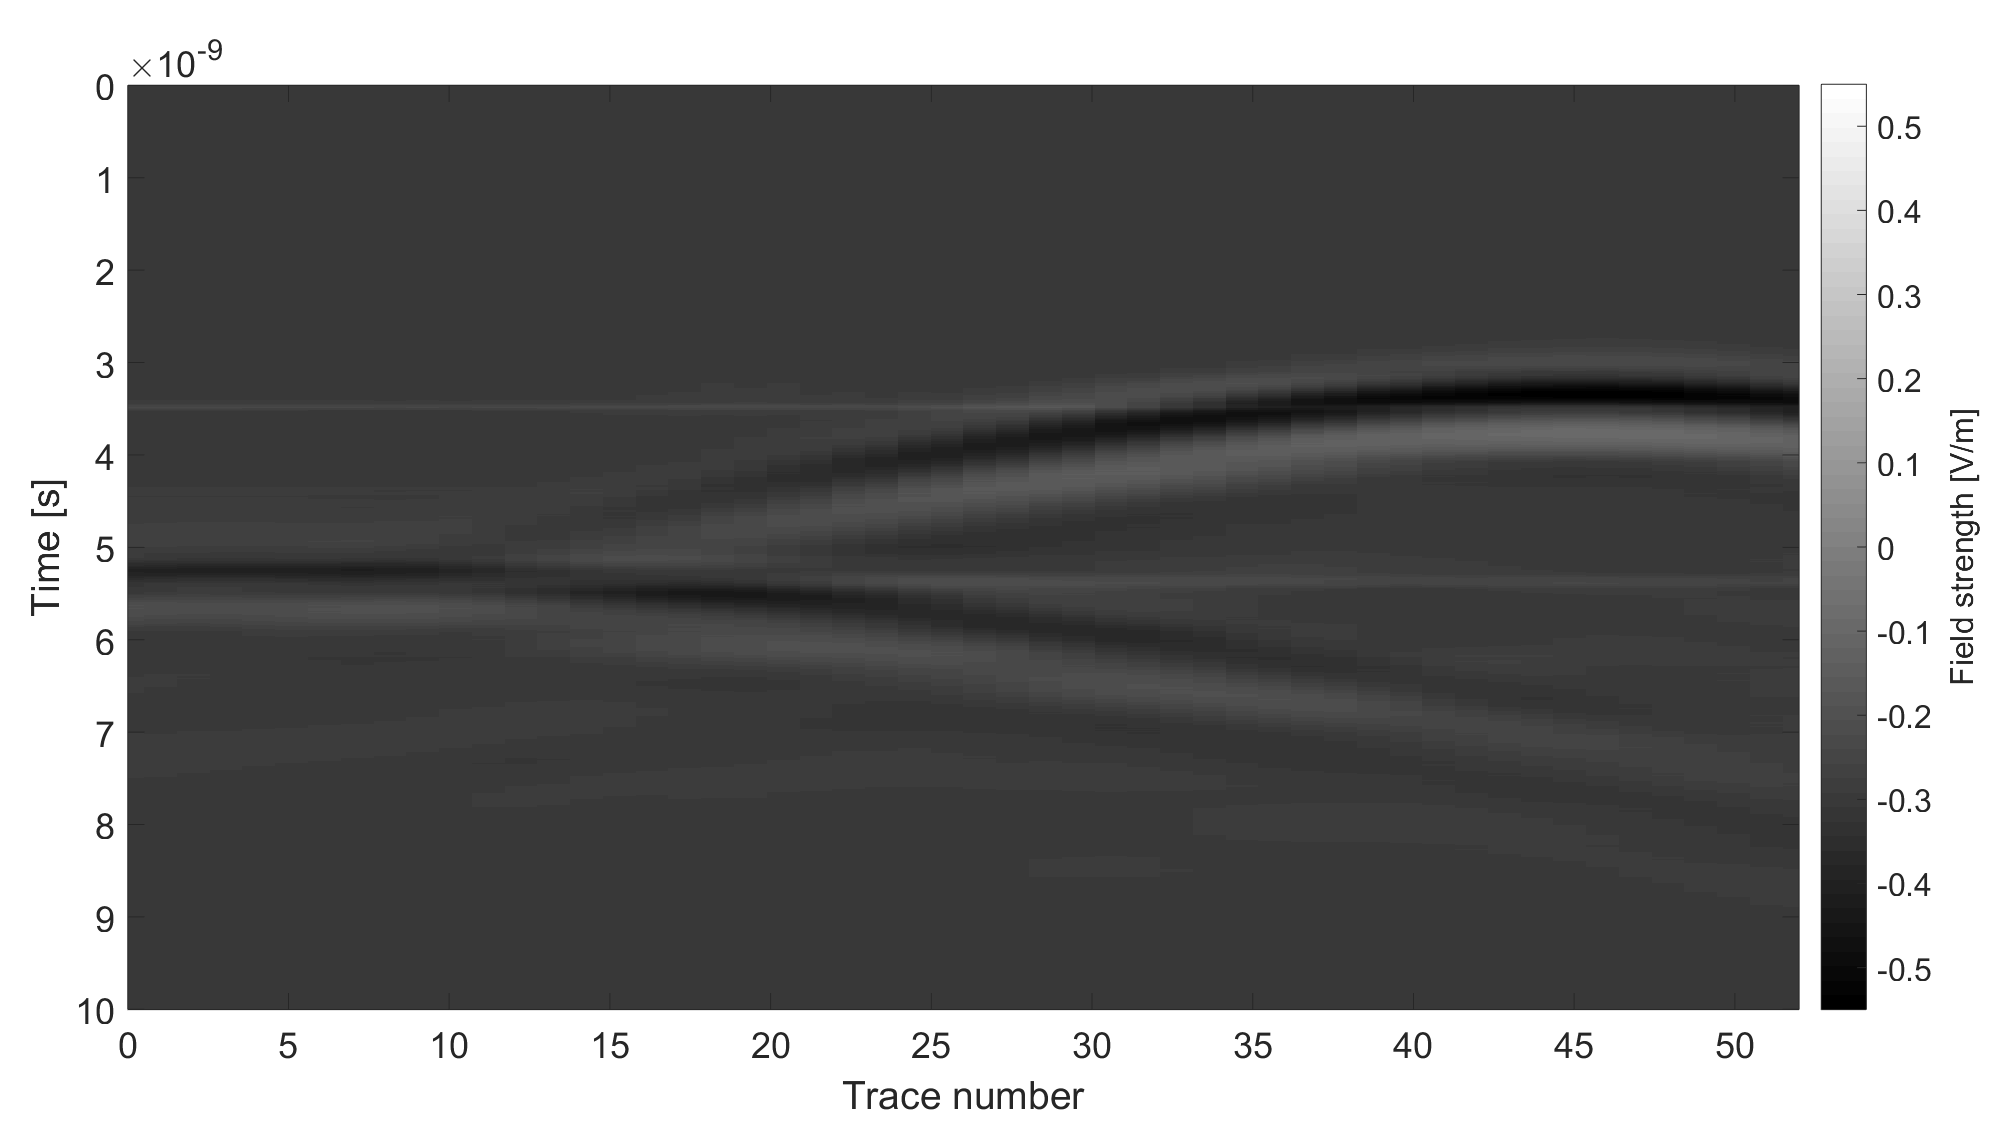
\includegraphics[width=0.47\textwidth, keepaspectratio,valign=c]{chapter2/images/mala_2_barras_bscan_sparse.png}
}

\caption{RPCA sobre trazas B en campo Ez}
\label{fig:bscanRPCA_SIM1}


\end{figure}

Para saber qué tan perfecta debe ser la señal extraída, se procede a realizar la simulación del mismo escenario pero sin barras metálicas. Al resultado de la traza B con todos los elementos le es restado la traza B con solo el suelo para tener como resultado la señal de las barras metálicas.

Para encontrar qué tan parecida es la señal de la traza B después de aplicar RPCA con la señal ``ideal''   matemáticamente podemos utilizar el índice de correlación.  Se realiza un programa en Matlab que permita cargar dos trazas B y a ellas le aplica el índice de correlación a todos los campos. Como resultado del ejemplo en medición se tiene:


\begin{table}[H]
\begin{center}
\caption{Similitud entre resultados aplicando RPCA} \label{tab:corrcoef1}
\begin{tabular}{l|c}
 & \multicolumn{1}{l}{\textbf{Índice de Correlación}} \\ \hline
\textbf{(Ex ideal,Ex Sparse)} & NaN \\
\textbf{(Ey ideal,Ey Sparse)} & 0.8482 \\
\textbf{(Ez ideal,Ez Sparse)} & 0.8482 \\
\textbf{(Hx ideal,Hx Sparse)} & 0.7593 \\
\textbf{(Hy ideal,Hy Sparse)} & 0.9670 \\
\textbf{(Hz ideal,Hz Sparse)} & 0.9703
\end{tabular}
\end{center}
\end{table} 

\begin{figure}[H]  
\centering
\subfigure[ Bscan Ideal ]{
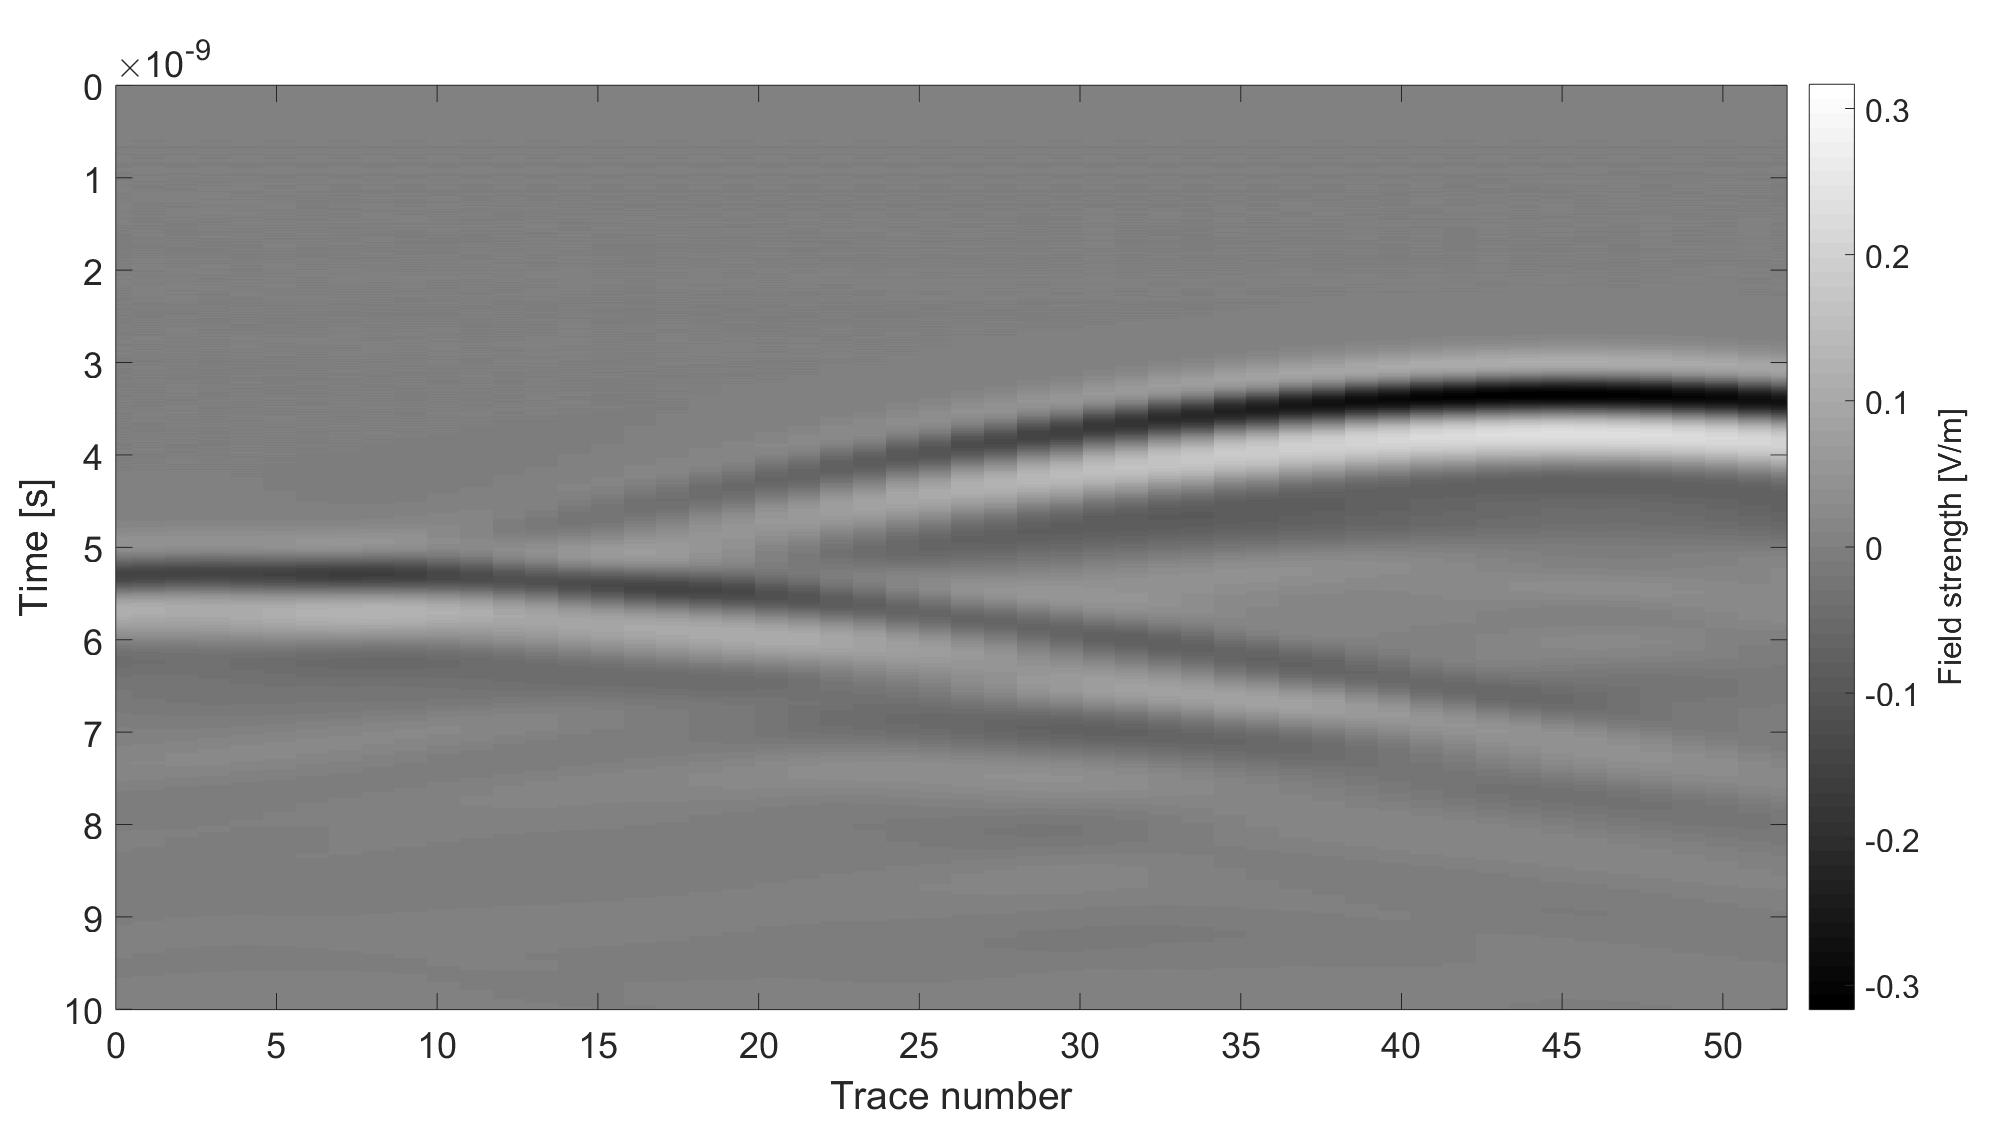
\includegraphics[width=0.47\textwidth, keepaspectratio,valign=c]{chapter2/images/mala_2_barras_bscan_sparse_ideal.png}
\label{fig:subfig2exampleCscan1GSSI}
}
\subfigure[Bscan Sparse ]{
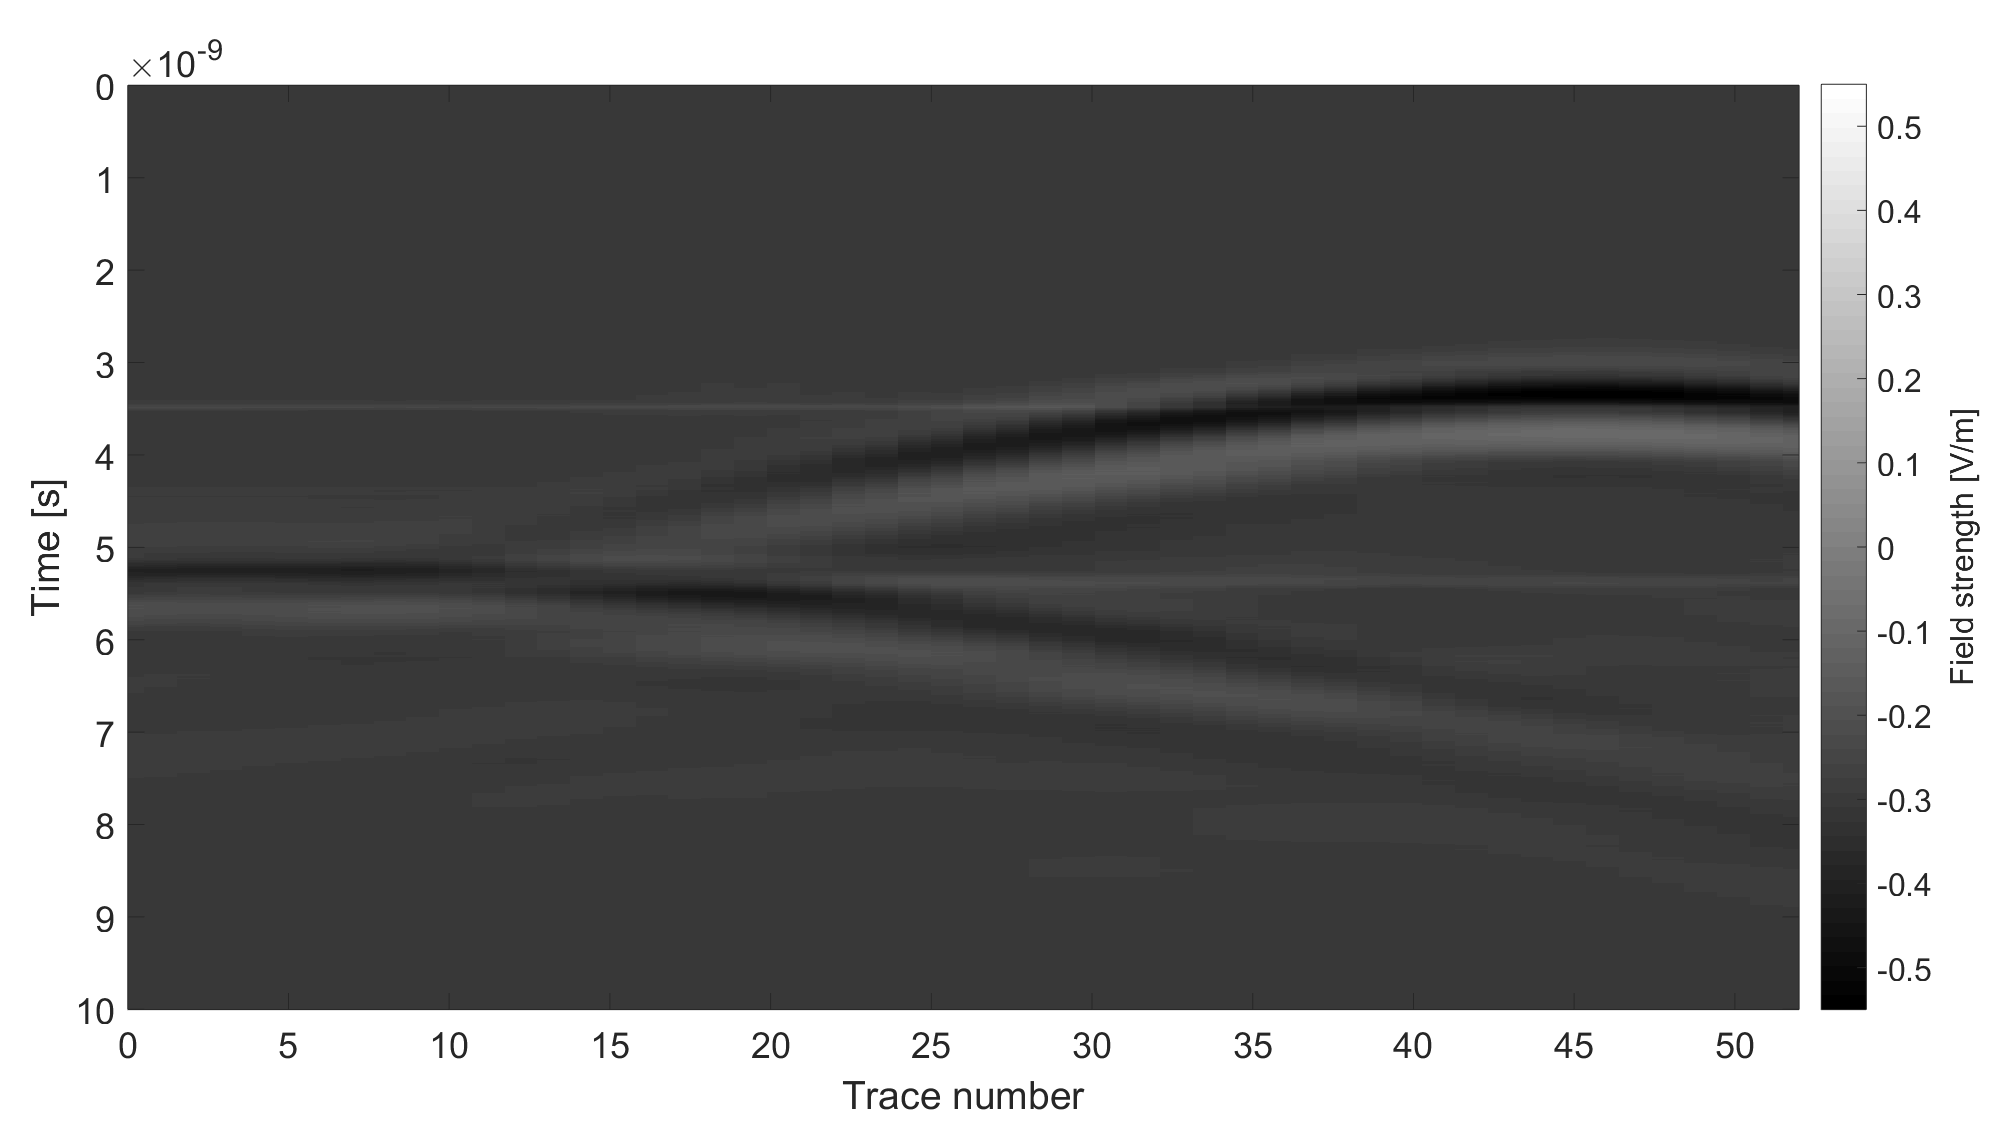
\includegraphics[width=0.47\textwidth, keepaspectratio,valign=c]{chapter2/images/mala_2_barras_bscan_sparse.png}
}

\caption{Señal Barras Metálicas Ez}
\label{fig:barraMetalIdeal}


\end{figure}

En la \figurename{ \ref{fig:barraMetalIdeal}} se puede observar la comparación de las señal ideal que debe generar únicamente las barras metálicas  con la señal resultante al aplicar RPCA.  Respecto a la \tablename{ \ref{tab:corrcoef1}} indica que la traza B (sparse) tiene una similitud del 84.8\% con respecto a la traza ideal.


\subsubsection{Mean Substraction}

Es uno  de los métodos de pre-procesamiento más simples para eliminar las componentes de baja frecuencia que se encuentran presentes en un conjunto de datos. \cite{round_Clutter_Removal_in_GPR_Surveys}. Se puede notar ${ e }_{ 1 }{ \left( t \right)  },{ e }_{ 2 }{ \left( t \right)  },{ e }_{ 3 }{ \left( t \right)  },...,{ e }_{ n }{ \left( t \right)  }$ como el conjunto de trazas A sobre M observaciones en un instante de tiempo t.  Cada traza contiene diferentes valores proveniente del acople entre antenas, la interferencia de las multiples señales de la interfaz aire-suelo y las señales reflejadas por los objetos enterrados (targets). La señal recolectada en una n-ésima posición puede ser notada como:

\begin{equation}
{ e }_{ n }{ \left( t \right)  }={ e }_{ na }{ \left( t \right)  }+{ e }_{ nw }{ \left( t \right)  }+{ e }_{ nt }{ \left( t \right)  }
\end{equation}

Donde ${ e }_{ na }{ \left( t \right)  }$ corresponde al acople entre antenas, ${ e }_{ nw }{ \left( t \right)  }$ la señal de las reflexiones del suelo y ${ e }_{ nt }{ \left( t \right)  }$ las reflexiones de los objetos.

Para aplicar este algoritmo se busca reducir o eliminar las componentes ${ e }_{ na }{ \left( t \right)  }$ y ${ e }_{ nw }{ \left( t \right)  }$ ya que son fuentes de ruido. Al eliminar las fuentes de ruido se puede tener una imagen ``mejorada'' de las señales originadas por los objetos enterrados.
La ecuación de este algoritmo de pre procesamiento  es:
\begin{equation}
{ e }_{ AVn }{ \left( t \right)  }={ e }_{ n }{ \left( t \right)  }-\quad \frac { 1 }{ M }  \sum _{ m=1 }^{ M }{ { e }_{ n }{ \left( t \right)  } } 
\end{equation}

Donde ${ e }_{ AVn }$ corresponde a valor de la traza extraída,  ${ e }_{ n }$ a los datos de la traza A en la n-ésima iteración y M el número de observaciones (Cuantas trazas A esta compuesta la traza B).
\newpage
\subsubsubsection{\textbf{Implementación Mean Substraction en trazas gprMax}}

Se desarrolló un programa en Matlab  para seleccionar un conjunto de trazas B y aplicarle a cada una de ellas el algoritmo Mean Substraction, el programa crea una carpeta nueva con los valores del resultado del algoritmo.

\begin{lstlisting}[ basicstyle=\tiny] 
% get_all_Bscans_MeanSubstraction.m
% Los Andes University
% Creaded By: Luis Eduardo Quibano Alarcon
% E-mail: le.quibano@uniandes.edu.co
% Description: This Script  opens a specific amoun of  Bscans in order to
%              apply them the MEAN SUBSTRACTION algotrithm in all field components of
%              each A-scaN.
% MeanSubstraction Algorithm: https://doi.org/10.1109/JSTARS.2013.2287016
%                             https://pdfs.semanticscholar.org/783c/70ff019d8f225ad9bc2aa61ba614f09628ba.pdf

clear all
close all
clc

[filename, pathname] = uigetfile('*.out', 'Select gprMax B-scans output files','MultiSelect','on');
fullfilename = strcat(pathname, filename);

filename = cellstr(filename);
pathname = cellstr(pathname);
fullfilename = cellstr(fullfilename);

%Extraigo todos los campos de los A-scan seleccionados y luego los guardo
%en la matriz del objeto fields{i}

fullfilenameMeanS = fullfilename;
filenameMeanS=filename;
%%CREATE A COPY OF B-SCAN WITH NAME LOW RANK
%%CREATE A COPY OF A-SCAN WITH NAME LOW RANK
if exist(strcat(pathname{1},'/MeanSubstraction')) == 7
    rmdir(strcat(pathname{1},'/MeanSubstraction'), 's')
end
mkdir(strcat(pathname{1},'/MeanSubstraction'))
pathToSave=strcat(pathname{1},'/MeanSubstraction')


for i=1:length(fullfilenameMeanS)
    if filename{i} ~= 0
        nameSplit = split(filenameMeanS{i},'.');
        nameSplit= nameSplit(1);
        nameSplit= strcat(pathToSave,'/',nameSplit{1});
        nameSplit=strcat(nameSplit(1:end),'_MeanS','.out');
        fullfilenameMeanS{i}=nameSplit ;
        copyfile(fullfilename{i}, nameSplit);
    end
end


if length(fullfilenameMeanS) ~=0
    for i=1:length(fullfilenameMeanS)
        if filename{i} ~= 0
            iterations = double(h5readatt(fullfilenameMeanS{i}, '/', 'Iterations'));
            dt = h5readatt(fullfilenameMeanS{i}, '/', 'dt');
            
            ExFieldPath = strcat('/rxs/rx1/', 'Ex');
            EyFieldPath = strcat('/rxs/rx1/', 'Ey');
            EzFieldPath = strcat('/rxs/rx1/', 'Ez');
            HxFieldPath = strcat('/rxs/rx1/', 'Hx');
            HyFieldPath = strcat('/rxs/rx1/', 'Hy');
            HzFieldPath = strcat('/rxs/rx1/', 'Hz');
            
            
            ExAllScans = h5read(fullfilenameMeanS{i}, ExFieldPath);
            tam = size(ExAllScans);
            longi= tam(1);
            EyAllScans = h5read(fullfilenameMeanS{i}, EyFieldPath);
            EzAllScans = h5read(fullfilenameMeanS{i}, EzFieldPath);
            HxAllScans = h5read(fullfilenameMeanS{i}, HxFieldPath);
            HyAllScans = h5read(fullfilenameMeanS{i}, HyFieldPath);
            HzAllScans = h5read(fullfilenameMeanS{i}, HzFieldPath);
            
            %Aplly Mean Substractions
            ExAllScansMeanS=  ExAllScans - sum((ExAllScans))/longi;
            EyAllScansMeanS=  EyAllScans - sum((EyAllScans))/longi;
            EzAllScansMeanS=  EzAllScans - sum((EzAllScans))/longi;
            HxAllScansMeanS=  HxAllScans - sum((HxAllScans))/longi;
            HyAllScansMeanS=  HyAllScans - sum((HyAllScans))/longi;
            HzAllScansMeanS=  HzAllScans - sum((HzAllScans))/longi;
 
            %Write in H5file
            h5write(fullfilenameMeanS{i}, ExFieldPath,ExAllScansMeanS);
            h5write(fullfilenameMeanS{i}, EyFieldPath,EyAllScansMeanS);
            h5write(fullfilenameMeanS{i}, EzFieldPath,EzAllScansMeanS);
            h5write(fullfilenameMeanS{i}, HxFieldPath,HxAllScansMeanS);
            h5write(fullfilenameMeanS{i}, HyFieldPath,HyAllScansMeanS);
            h5write(fullfilenameMeanS{i}, HzFieldPath,HzAllScansMeanS);
            
            
        end
    end
    
end

\end{lstlisting}


\begin{figure}[H]  
\centering
\subfigure[ Modelo Original ]{
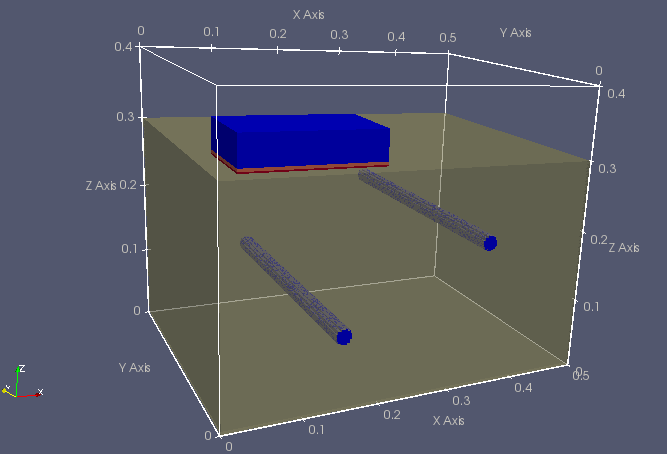
\includegraphics[width=0.25\textwidth, keepaspectratio,valign=c]{chapter2/images/mala_2_barras.png}
\label{fig:subfig_mala2_barras_mod}
}\\
\subfigure[ Bscan datos originales ]{
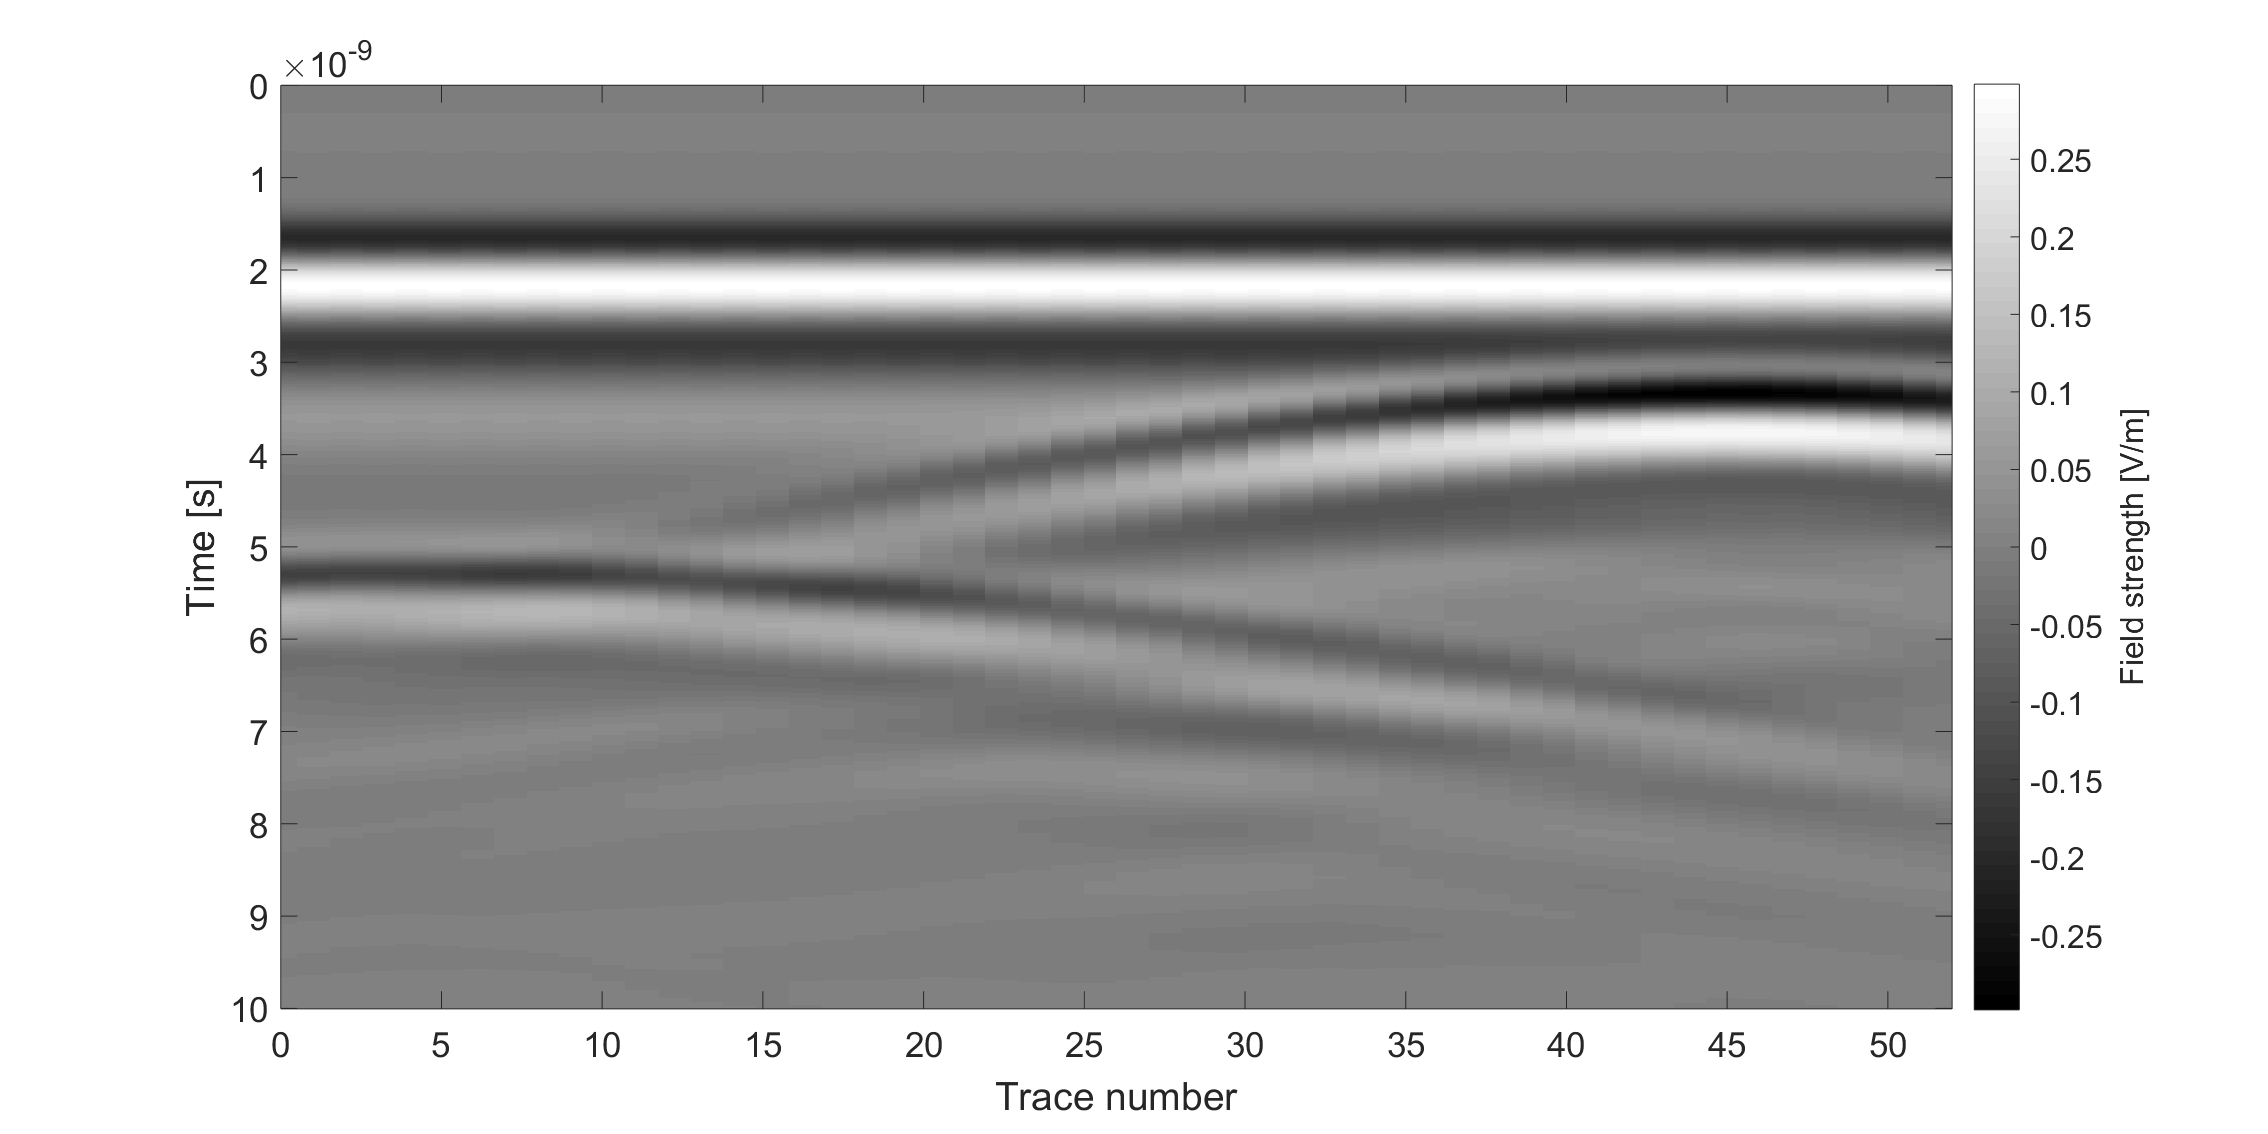
\includegraphics[width=0.45\textwidth, keepaspectratio,valign=c]{chapter2/images/mala_2_barras_bscan.png}
\label{fig:subfig1xampleCscan1GSSI}
}
\subfigure[ Bscan Mean Substraction ]{
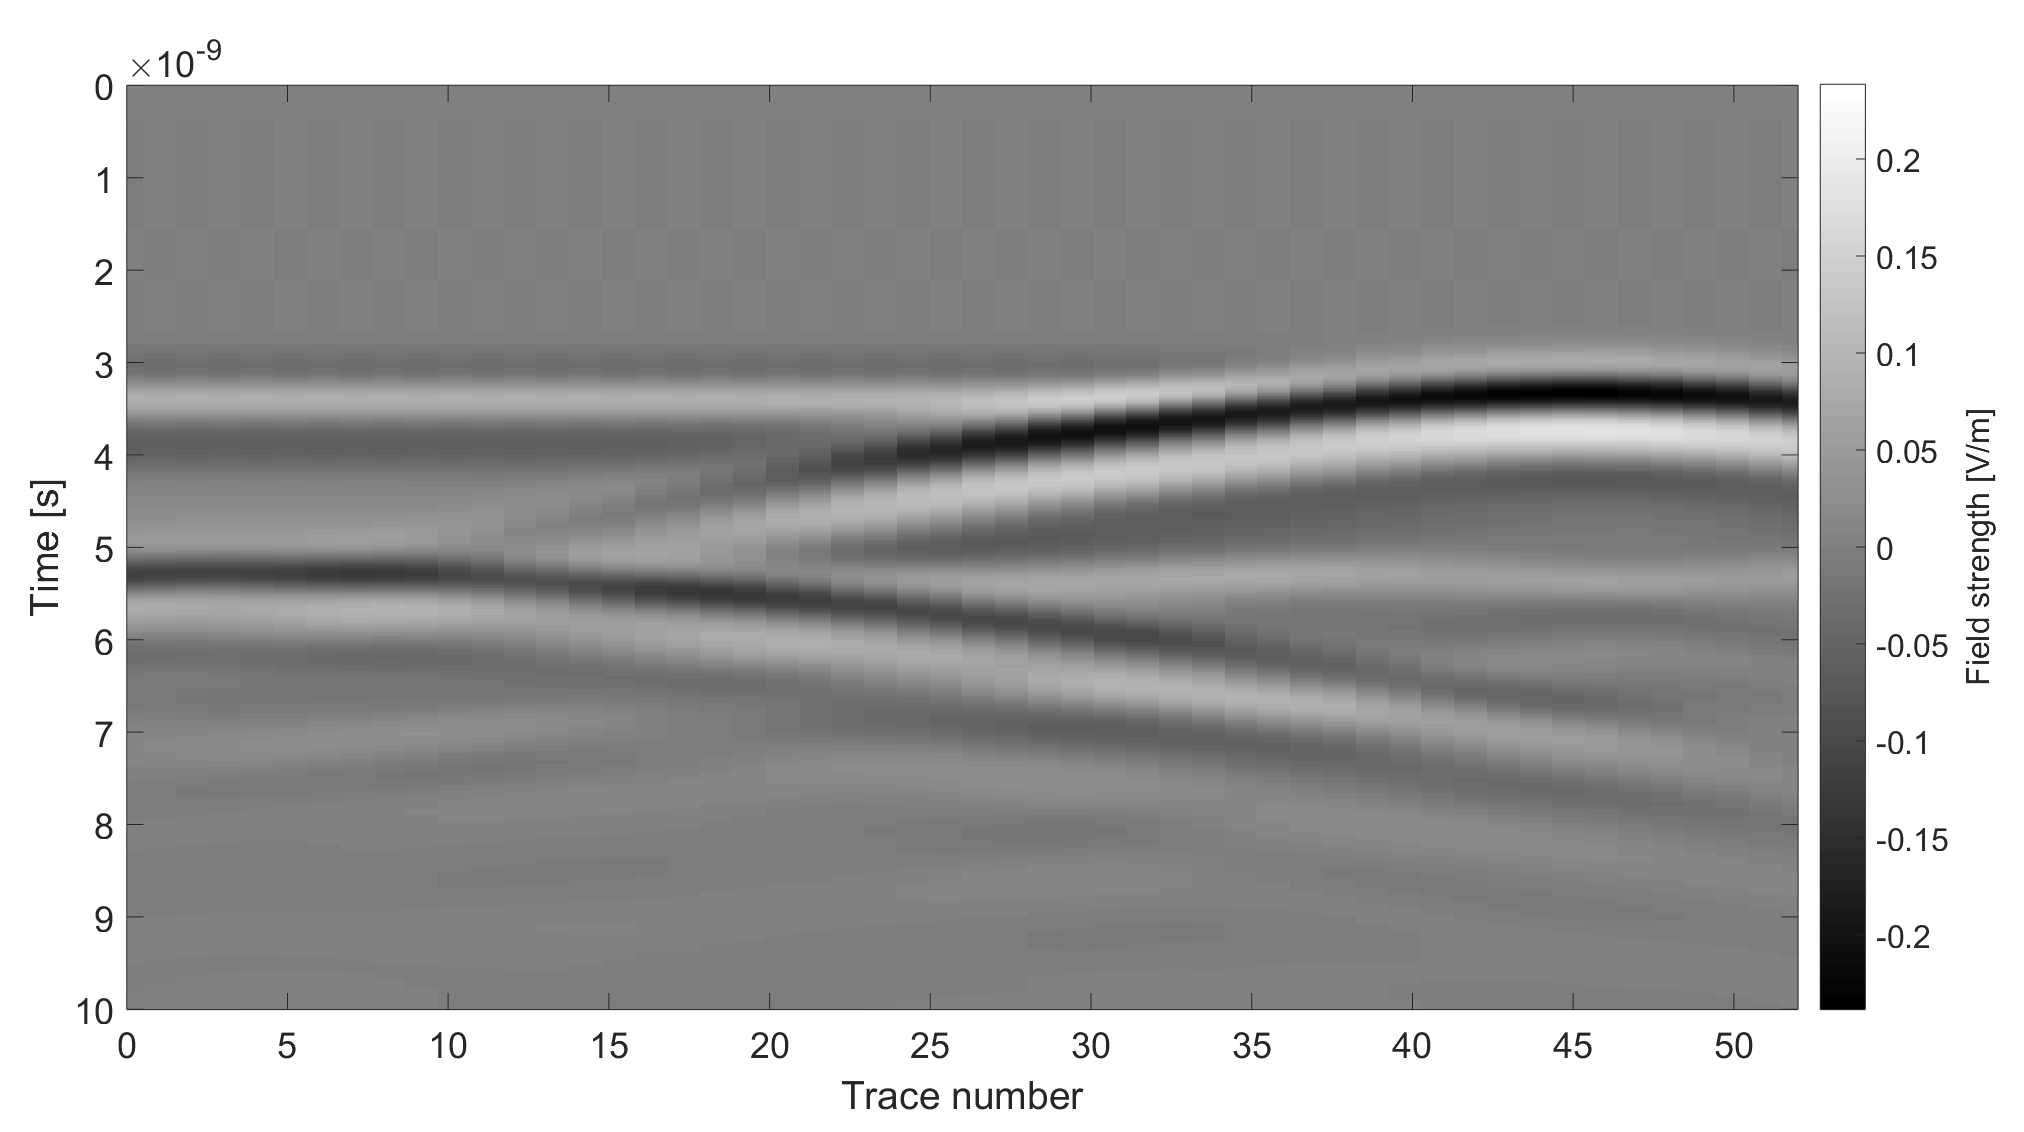
\includegraphics[width=0.45\textwidth, keepaspectratio,valign=c]{chapter2/images/mala_2_barras_bscan_meanSubstraction.png}
\label{fig:subfig2exampleCscan1GSSI}
}
\caption{Mean Substraction sobre trazas B en campo Ez}
\label{fig:bscanMeanSubs1}
\end{figure}


\begin{table}[H]
\begin{center}
\caption{Similitud entre resultados aplicando Mean Subtraction} \label{tab:corrcoefMean}
\begin{tabular}{l|c}
 & \multicolumn{1}{l}{\textbf{Índice de Correlación}} \\ \hline
\textbf{(Ex ideal,Ex MeanS)} & NaN \\
\textbf{(Ey ideal,Ey MeanS)} & 0.8015 \\
\textbf{(Ez ideal,Ez MeanS)} & 0.8016 \\
\textbf{(Hx ideal,Hx MeanS)} & 0.7684 \\
\textbf{(Hy ideal,Hy MeanS)} & 0.8580 \\
\textbf{(Hz ideal,Hz MeanS)} & 0.8639
\end{tabular}
\end{center}
\end{table} 


\begin{figure}[H]  
\centering
\subfigure[ Bscan Ideal ]{
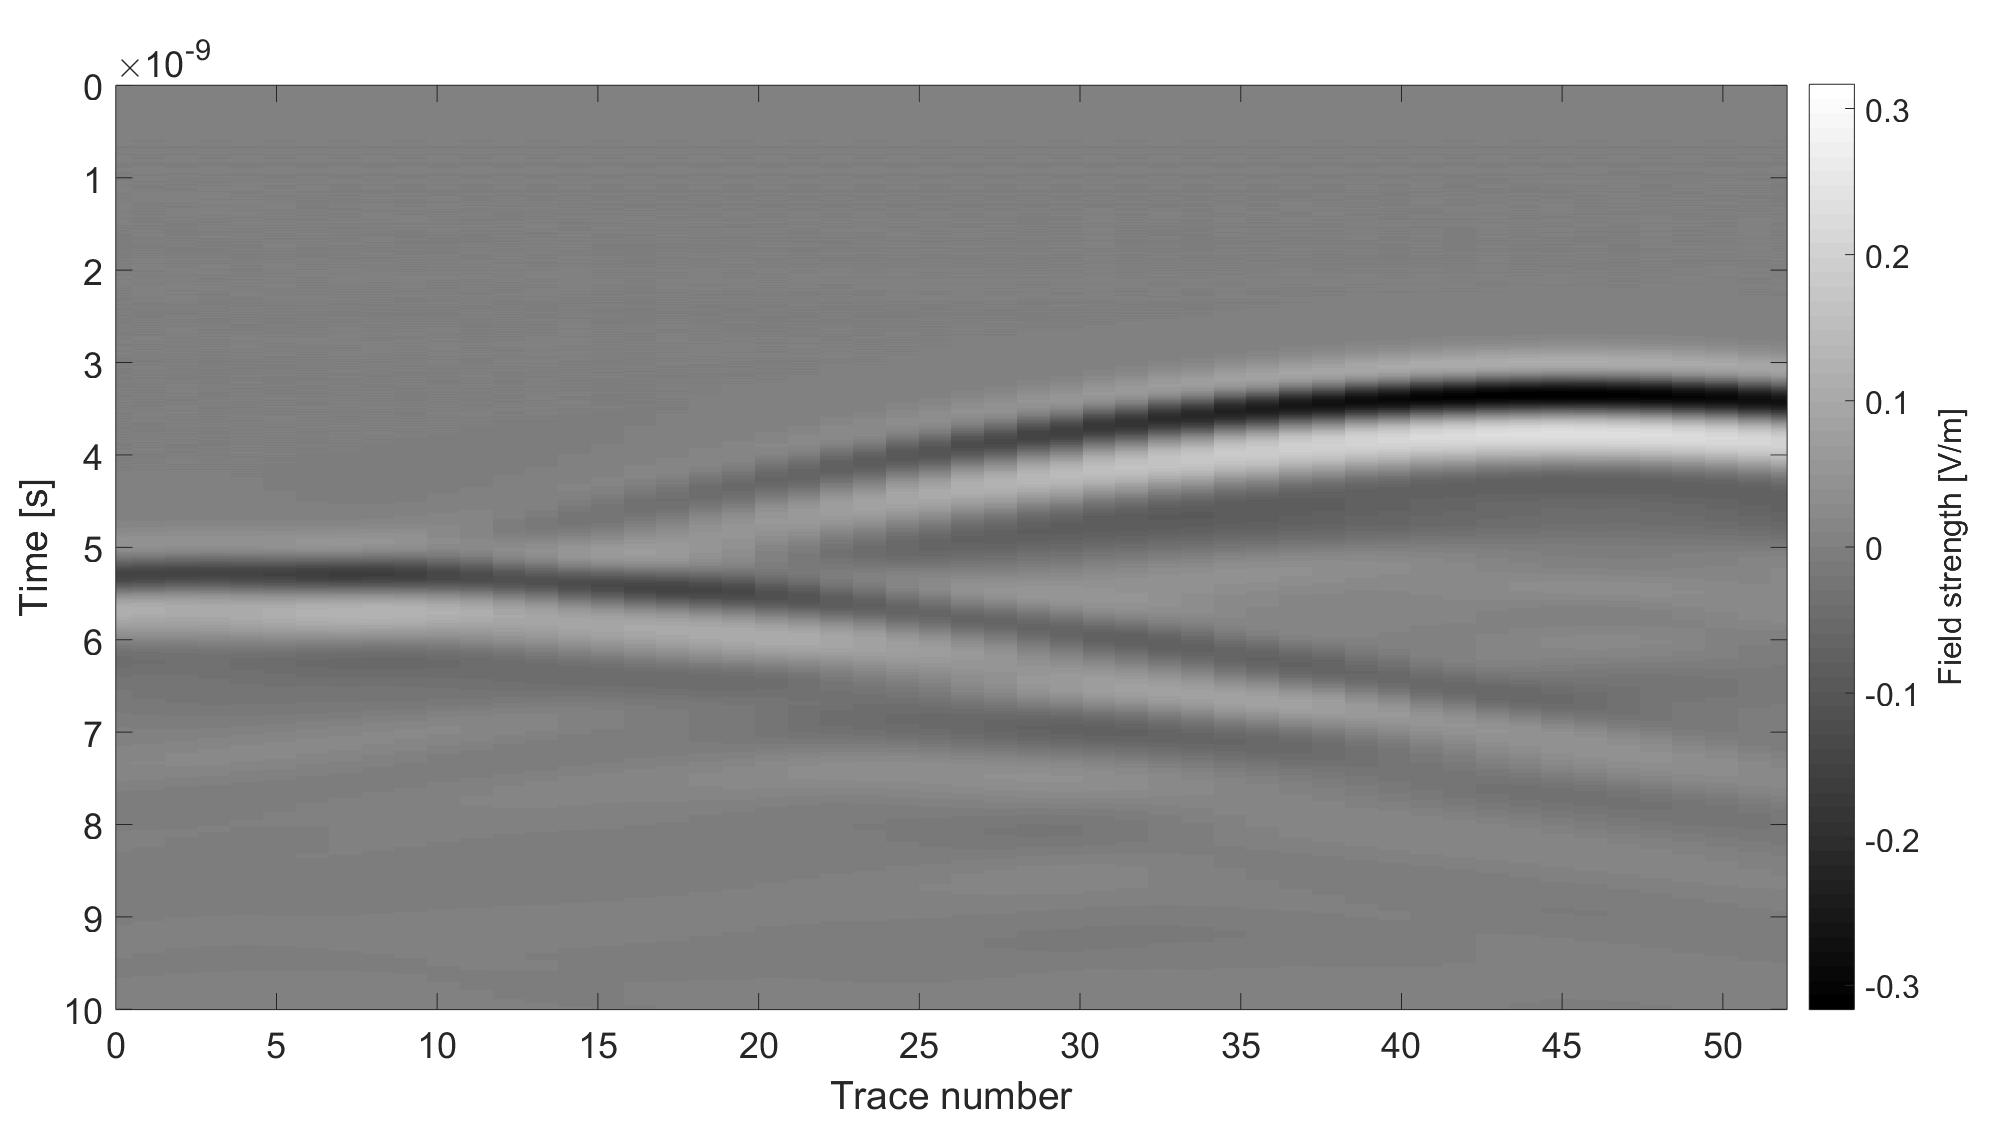
\includegraphics[width=0.47\textwidth, keepaspectratio,valign=c]{chapter2/images/mala_2_barras_bscan_sparse_ideal.png}
\label{fig:subfig2exampleCscan1GSSI}
}
\subfigure[Bscan Mean Substraction ]{
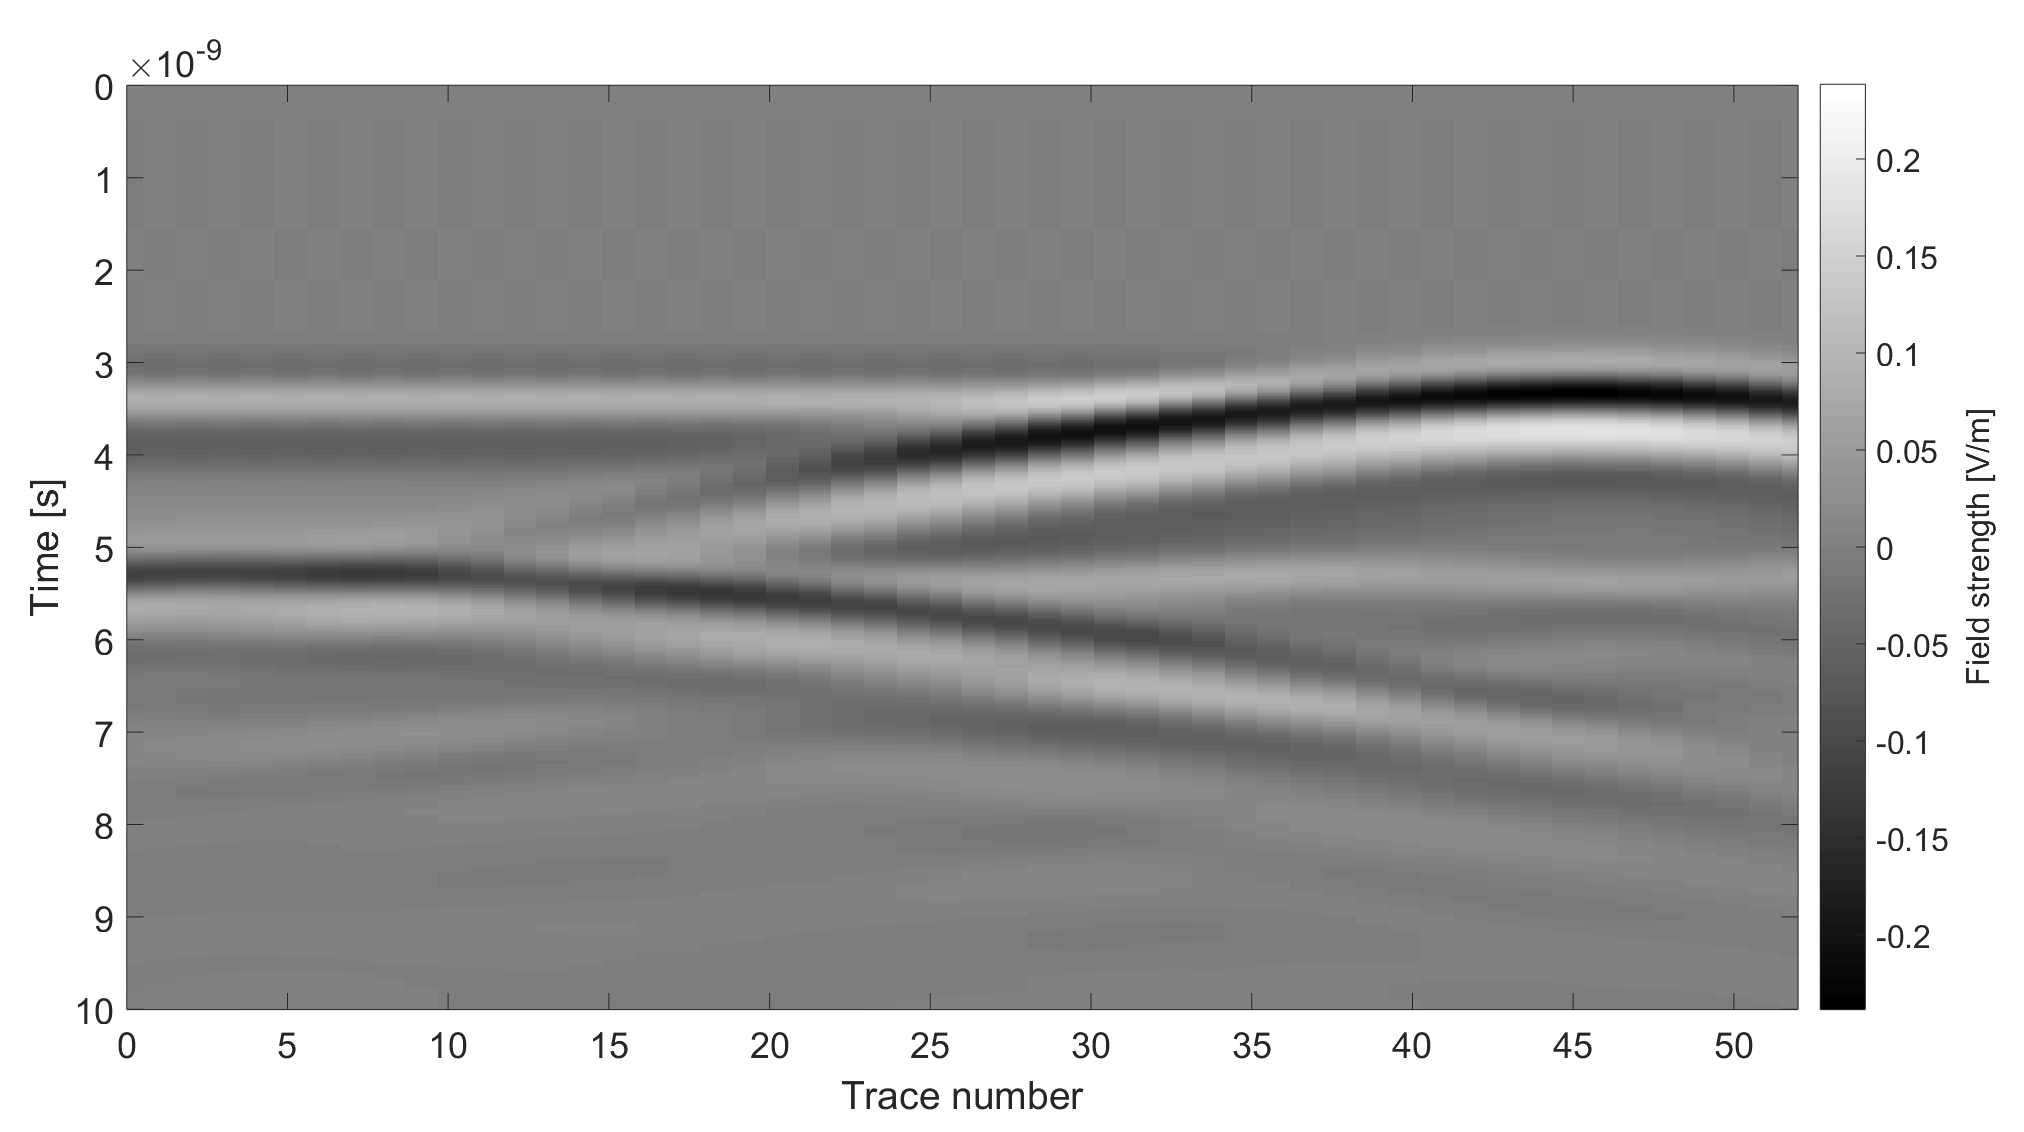
\includegraphics[width=0.47\textwidth, keepaspectratio,valign=c]{chapter2/images/mala_2_barras_bscan_meanSubstraction.png}
}
\caption{Señal Barras Metálicas Ez}
\label{fig:barraMetalIdeal}
\end{figure}

 
\subsubsection{Contrast Stretching}

\subsubsection{Entropy Based-Time Gating}
\subsubsection{Subspace Projection}





\section{Implementación Algoritmos}


\subsection{Resultados de la implementación}

\subsubsection{Escenario 001}
\subsubsubsection{Descripción}
\begin{figure}[H]
\centering
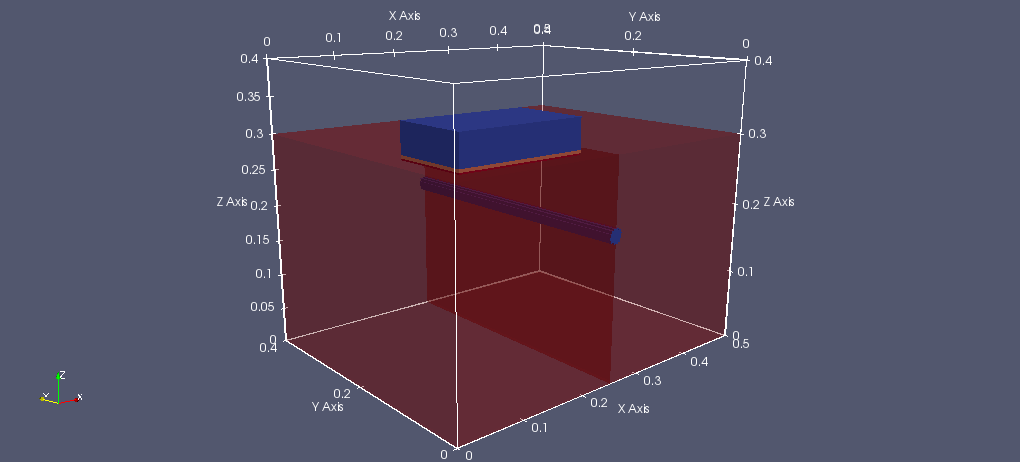
\includegraphics[height=5cm,keepaspectratio]{Homogeneo/001.png}
\caption{Modelo 3D del escenario 001 gprMax }
\label{fig:001_MODELO}
\end{figure}



\subsubsubsection{Datos Originales}
\begin{center}
\CT
\subfloat{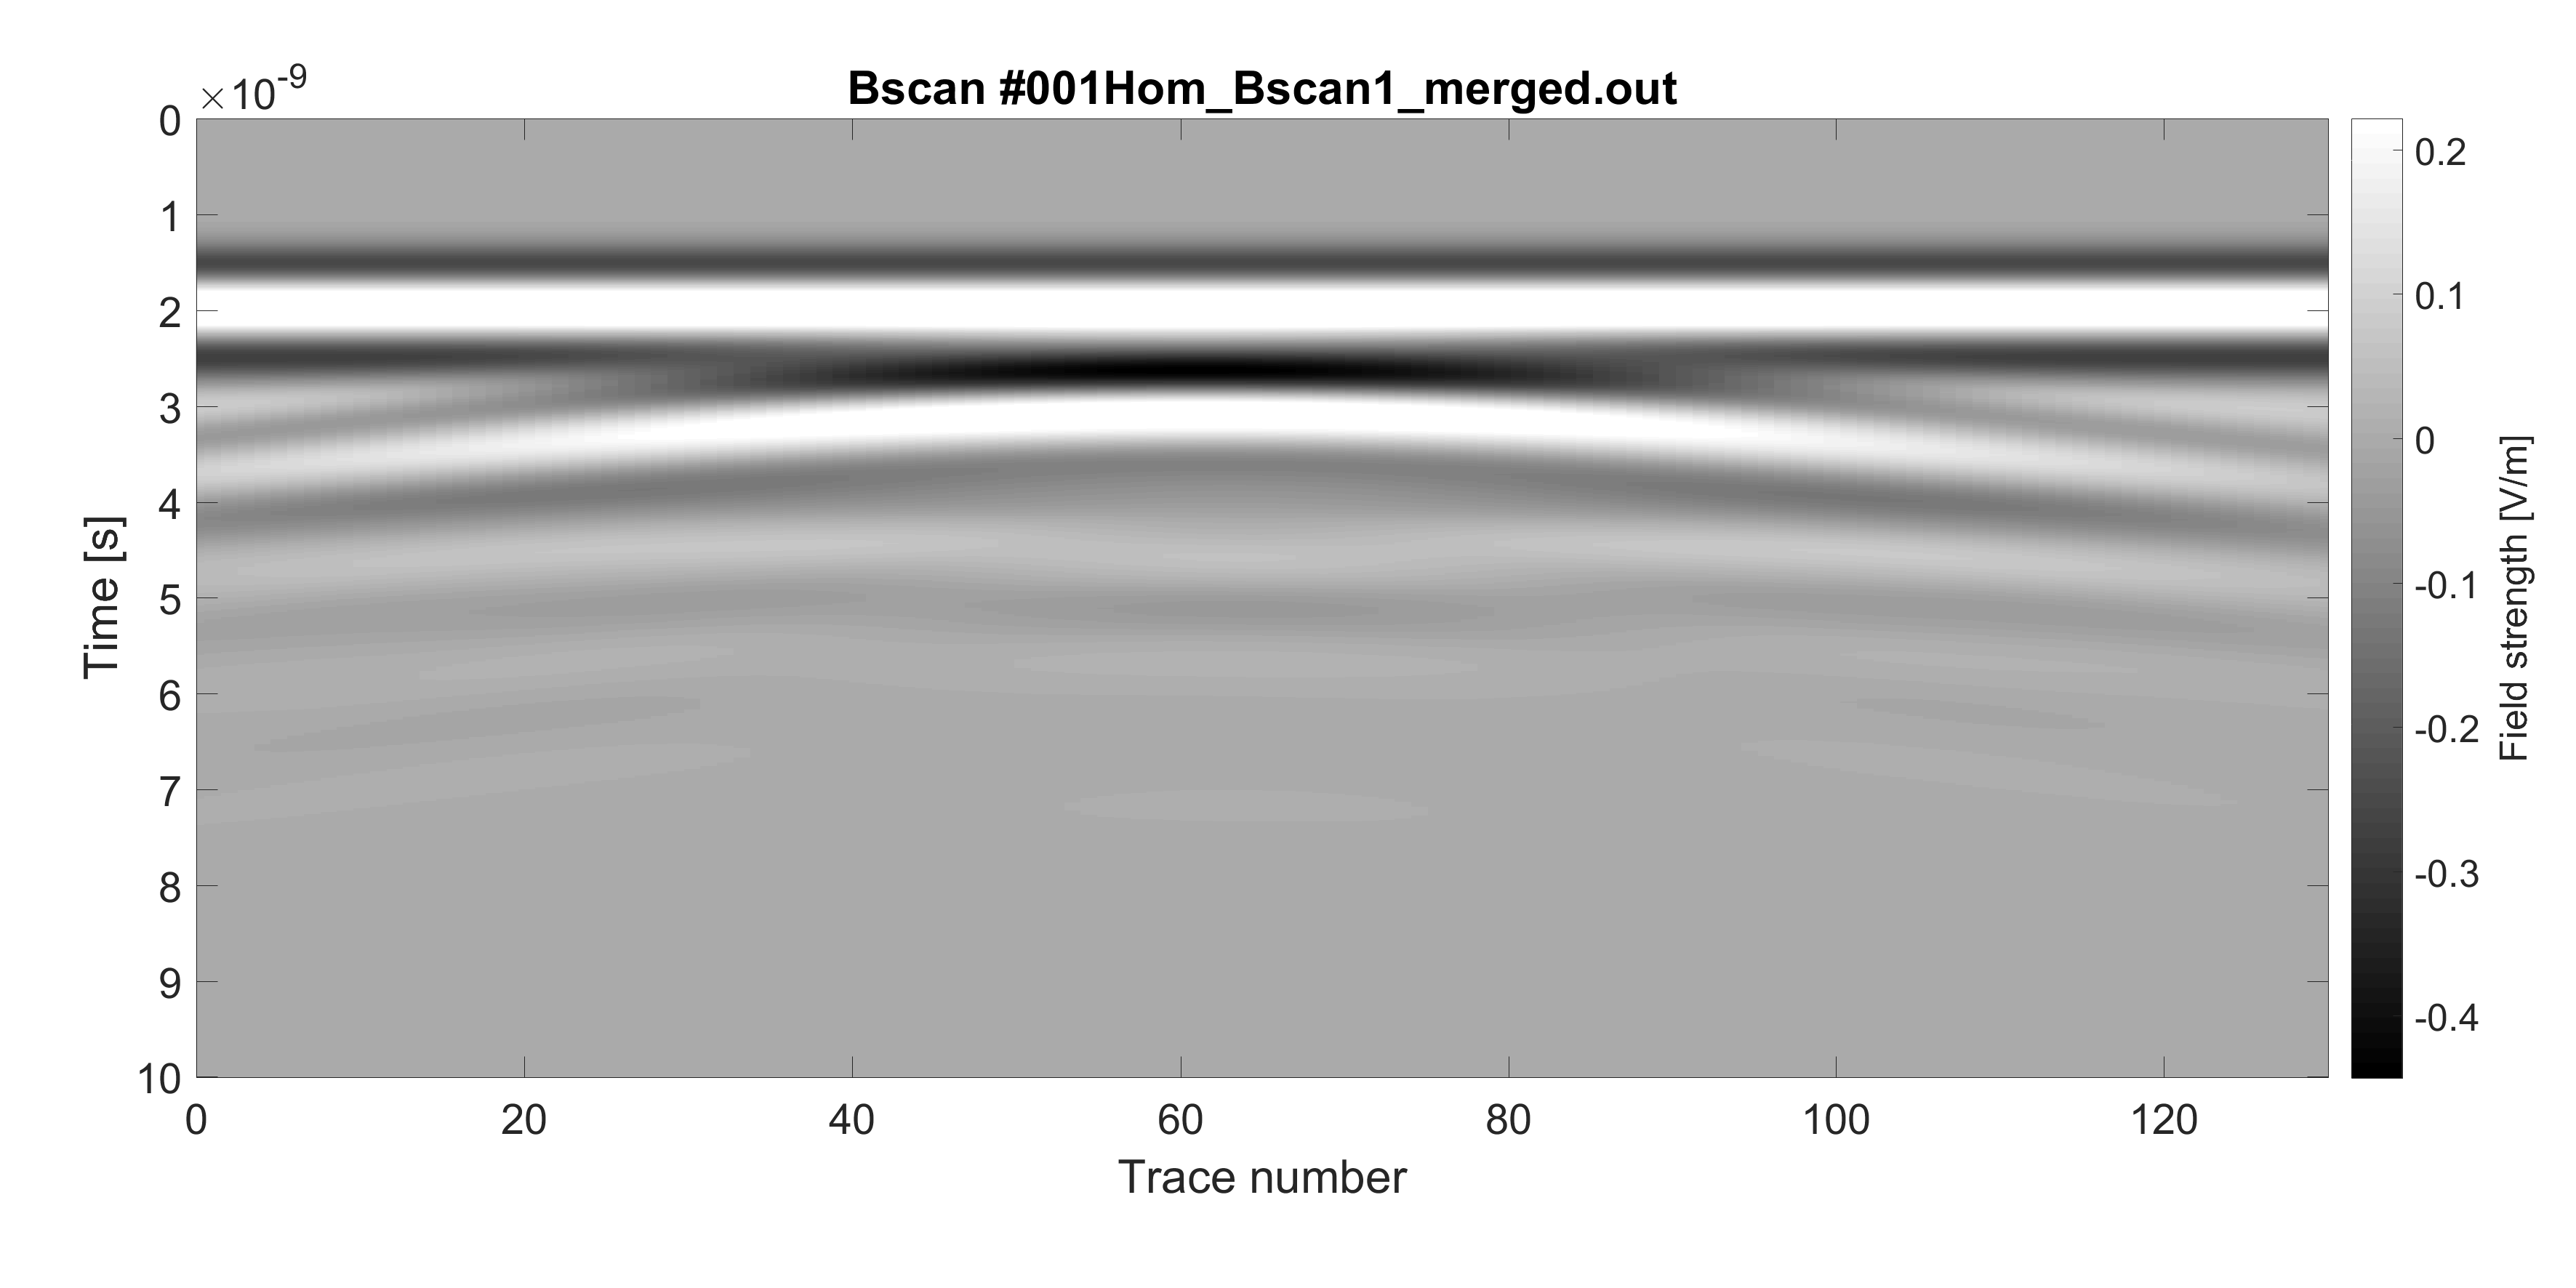
\includegraphics[width=0.47\textwidth, keepaspectratio,valign=c]{Homogeneo/001Hom_Bscan1_merged.png}}
\subfloat{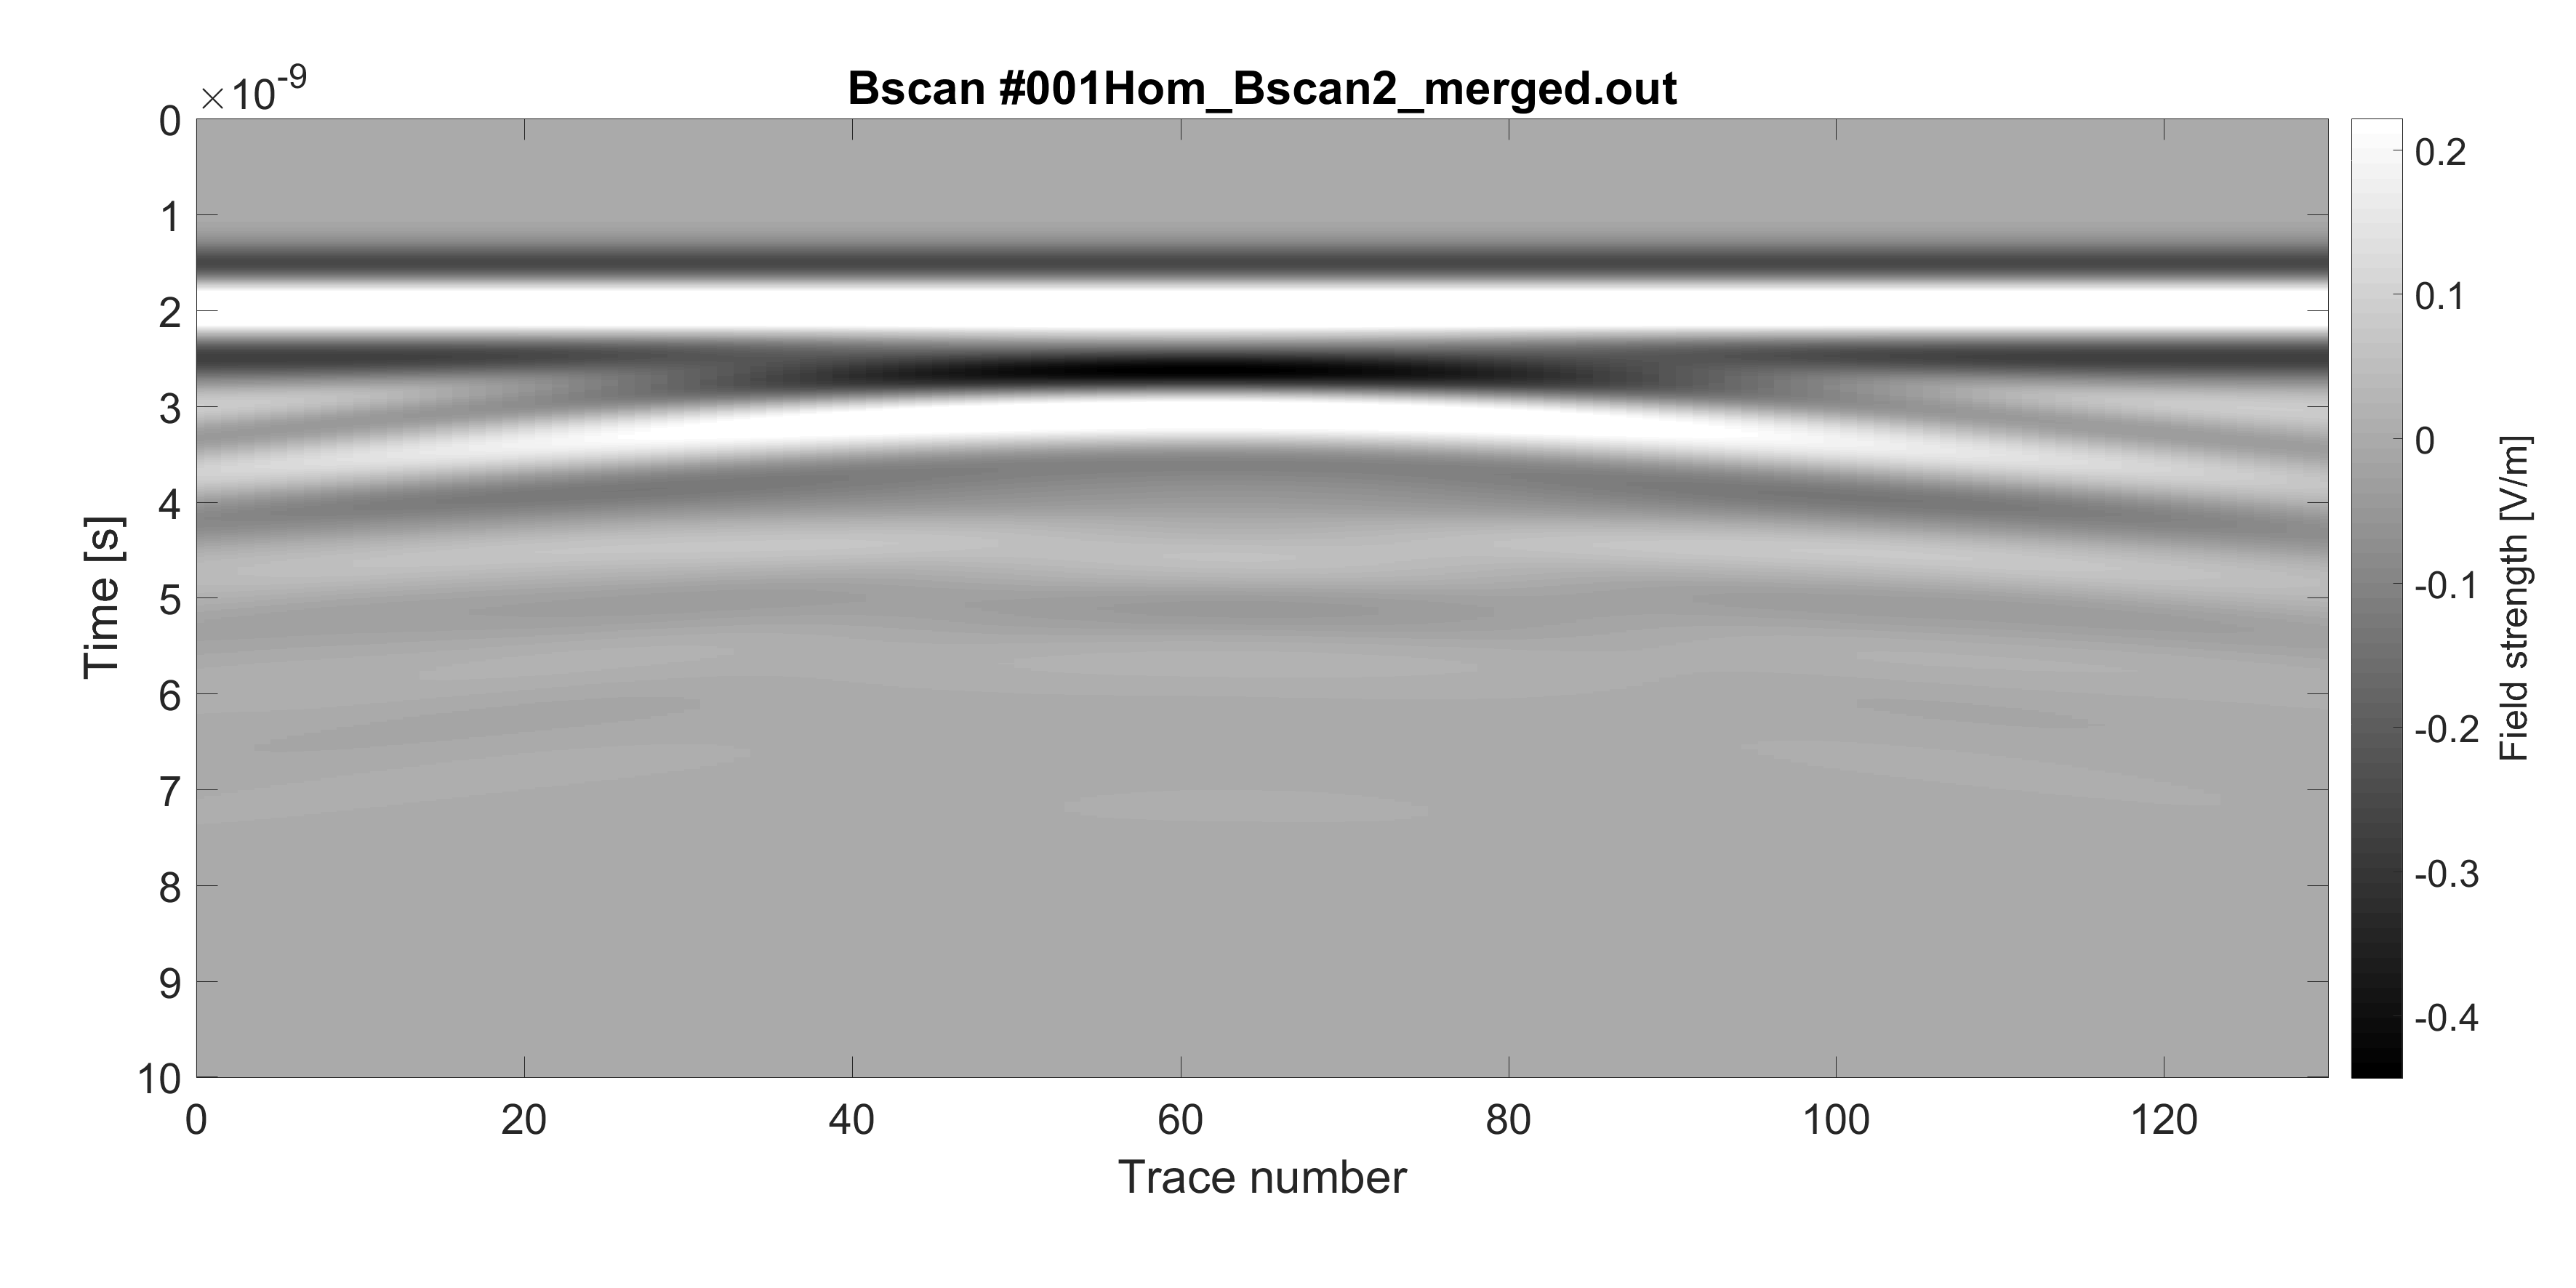
\includegraphics[width=0.47\textwidth, keepaspectratio,valign=c]{Homogeneo/001Hom_Bscan2_merged.png}}
\subfloat{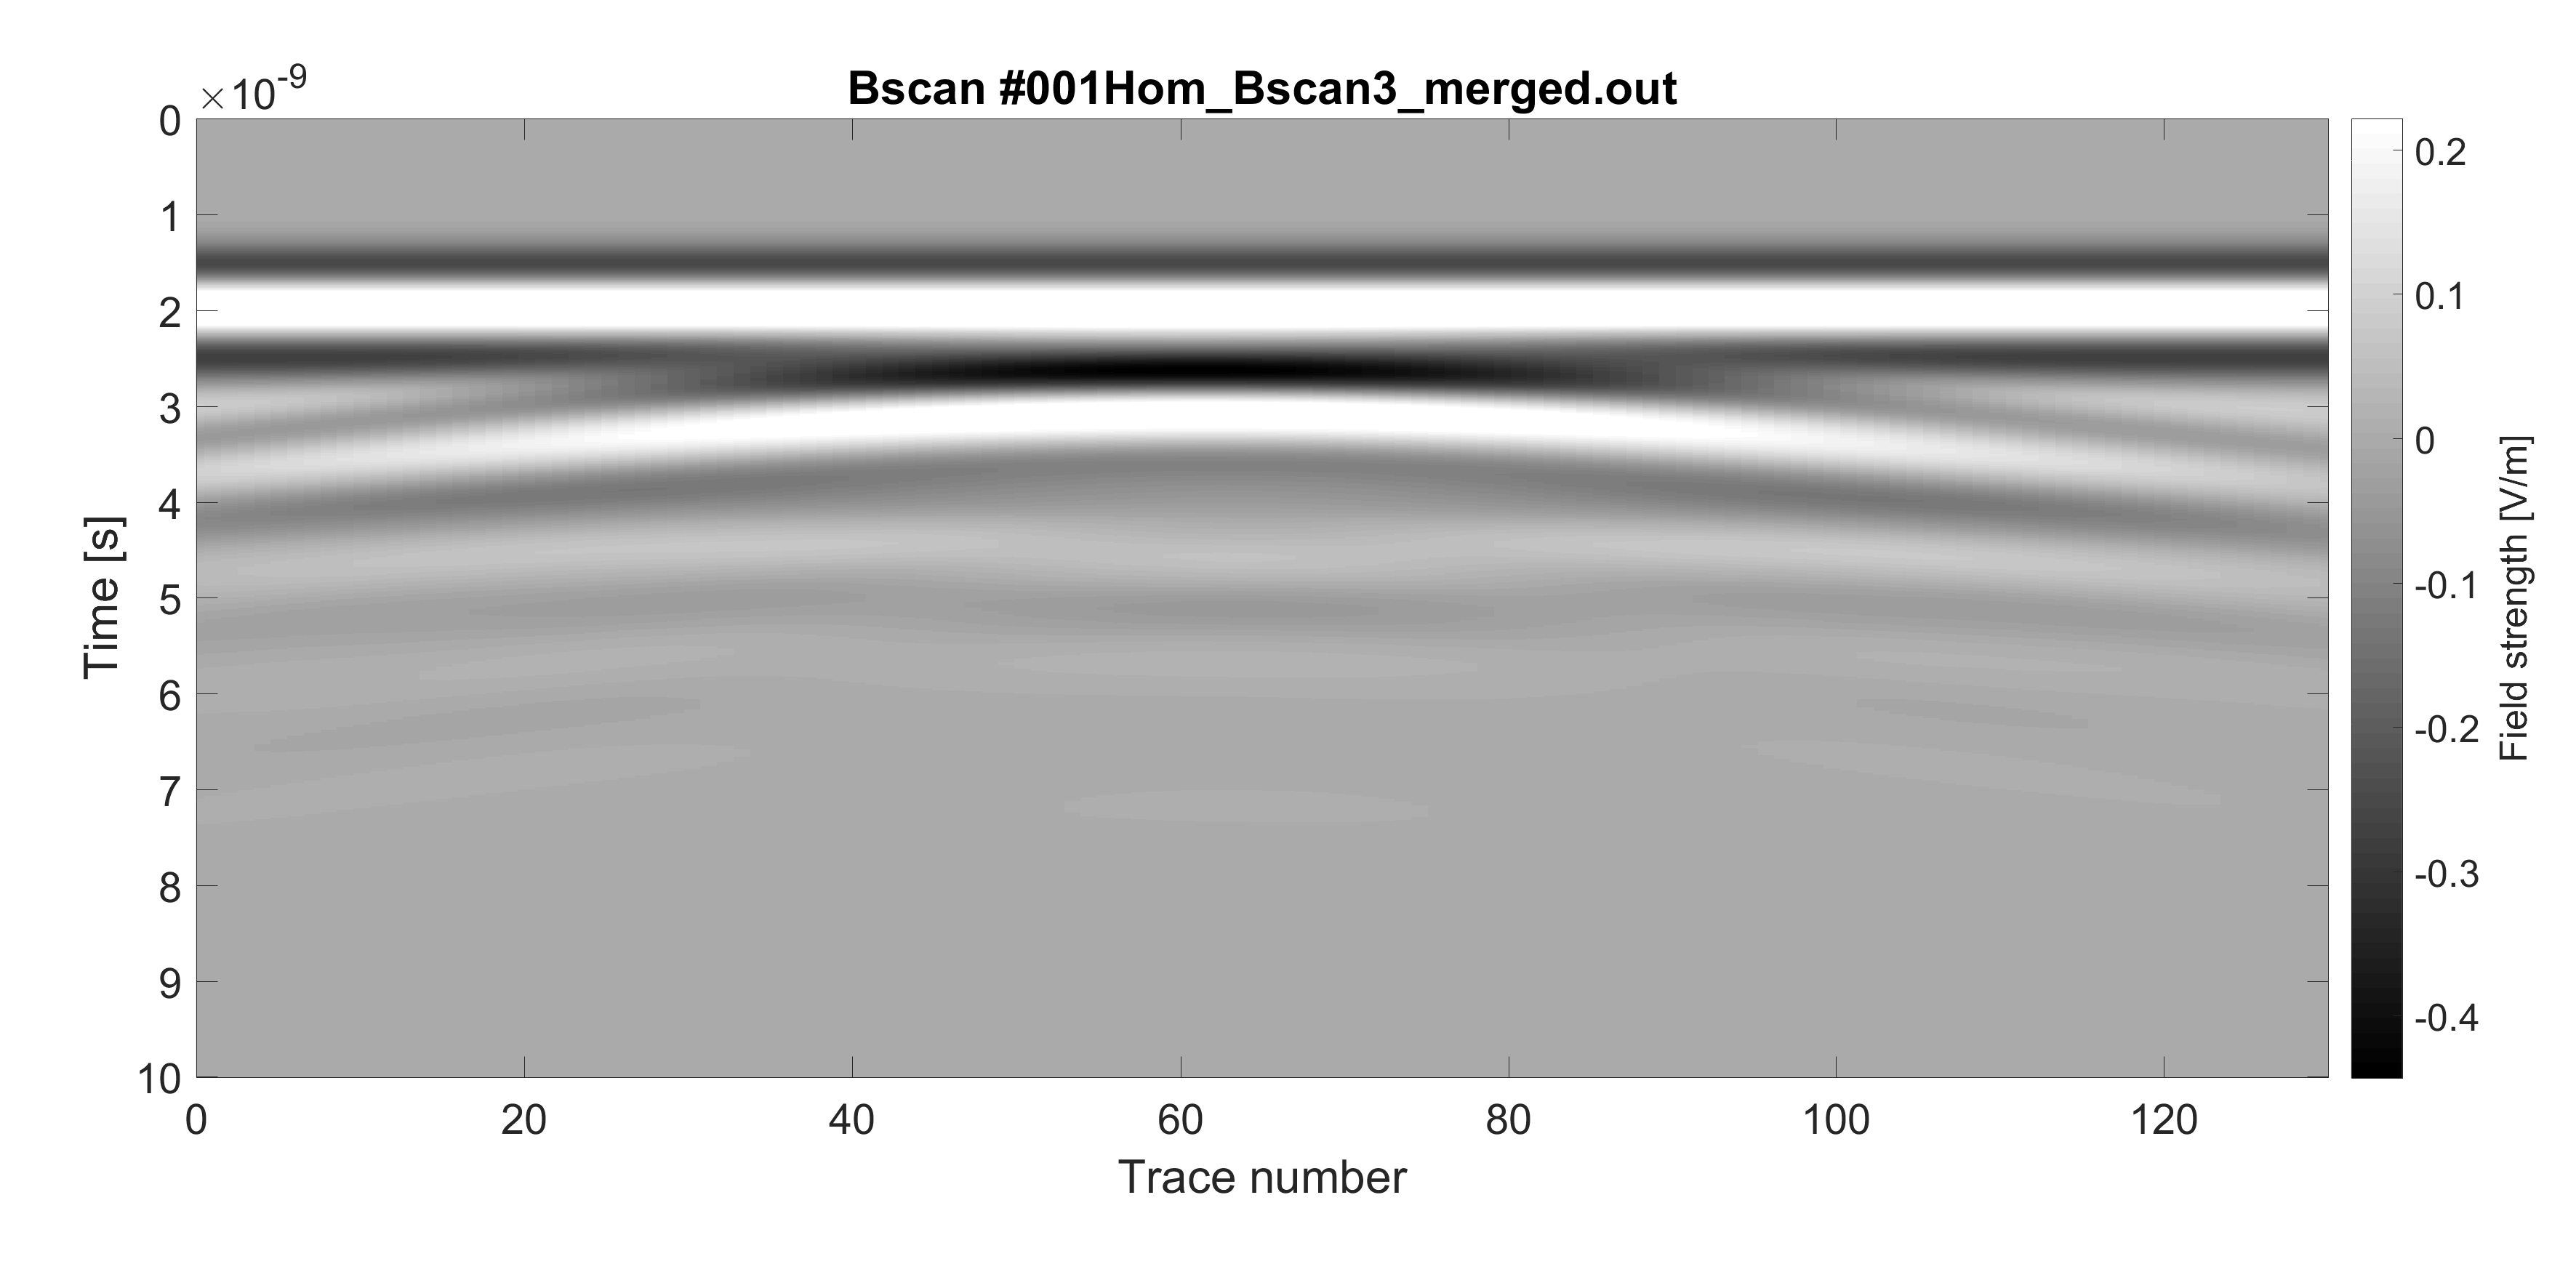
\includegraphics[width=0.47\textwidth, keepaspectratio,valign=c]{Homogeneo/001Hom_Bscan3_merged.png}}
\subfloat{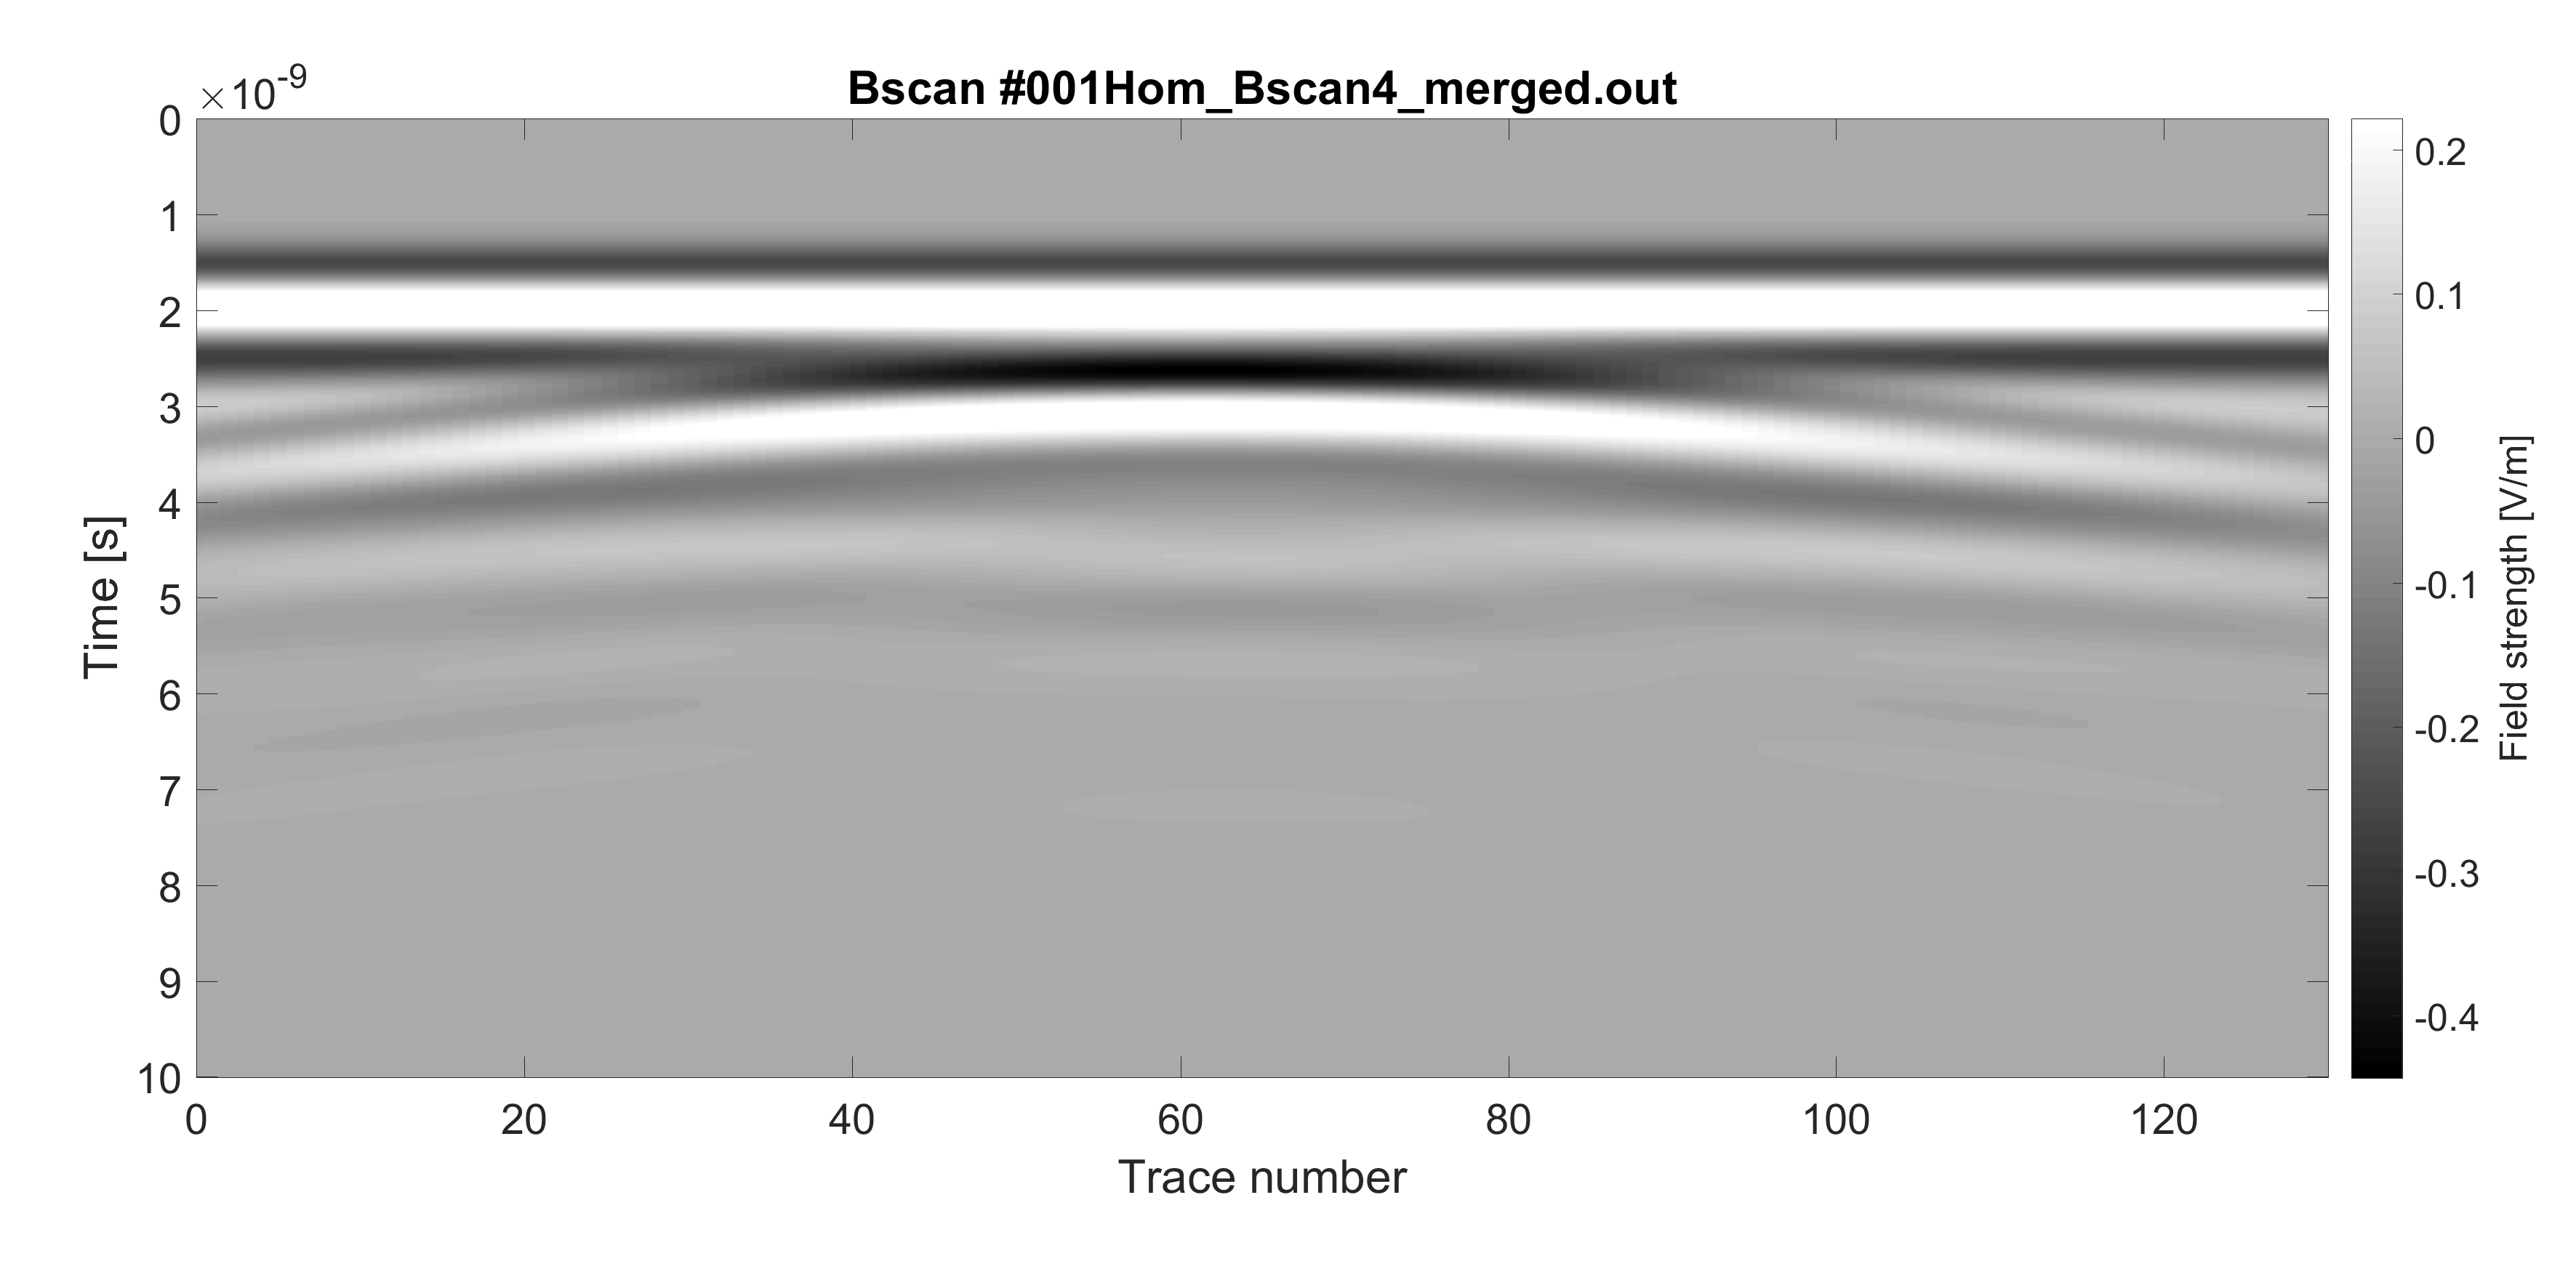
\includegraphics[width=0.47\textwidth, keepaspectratio,valign=c]{Homogeneo/001Hom_Bscan4_merged.png}}
\subfloat{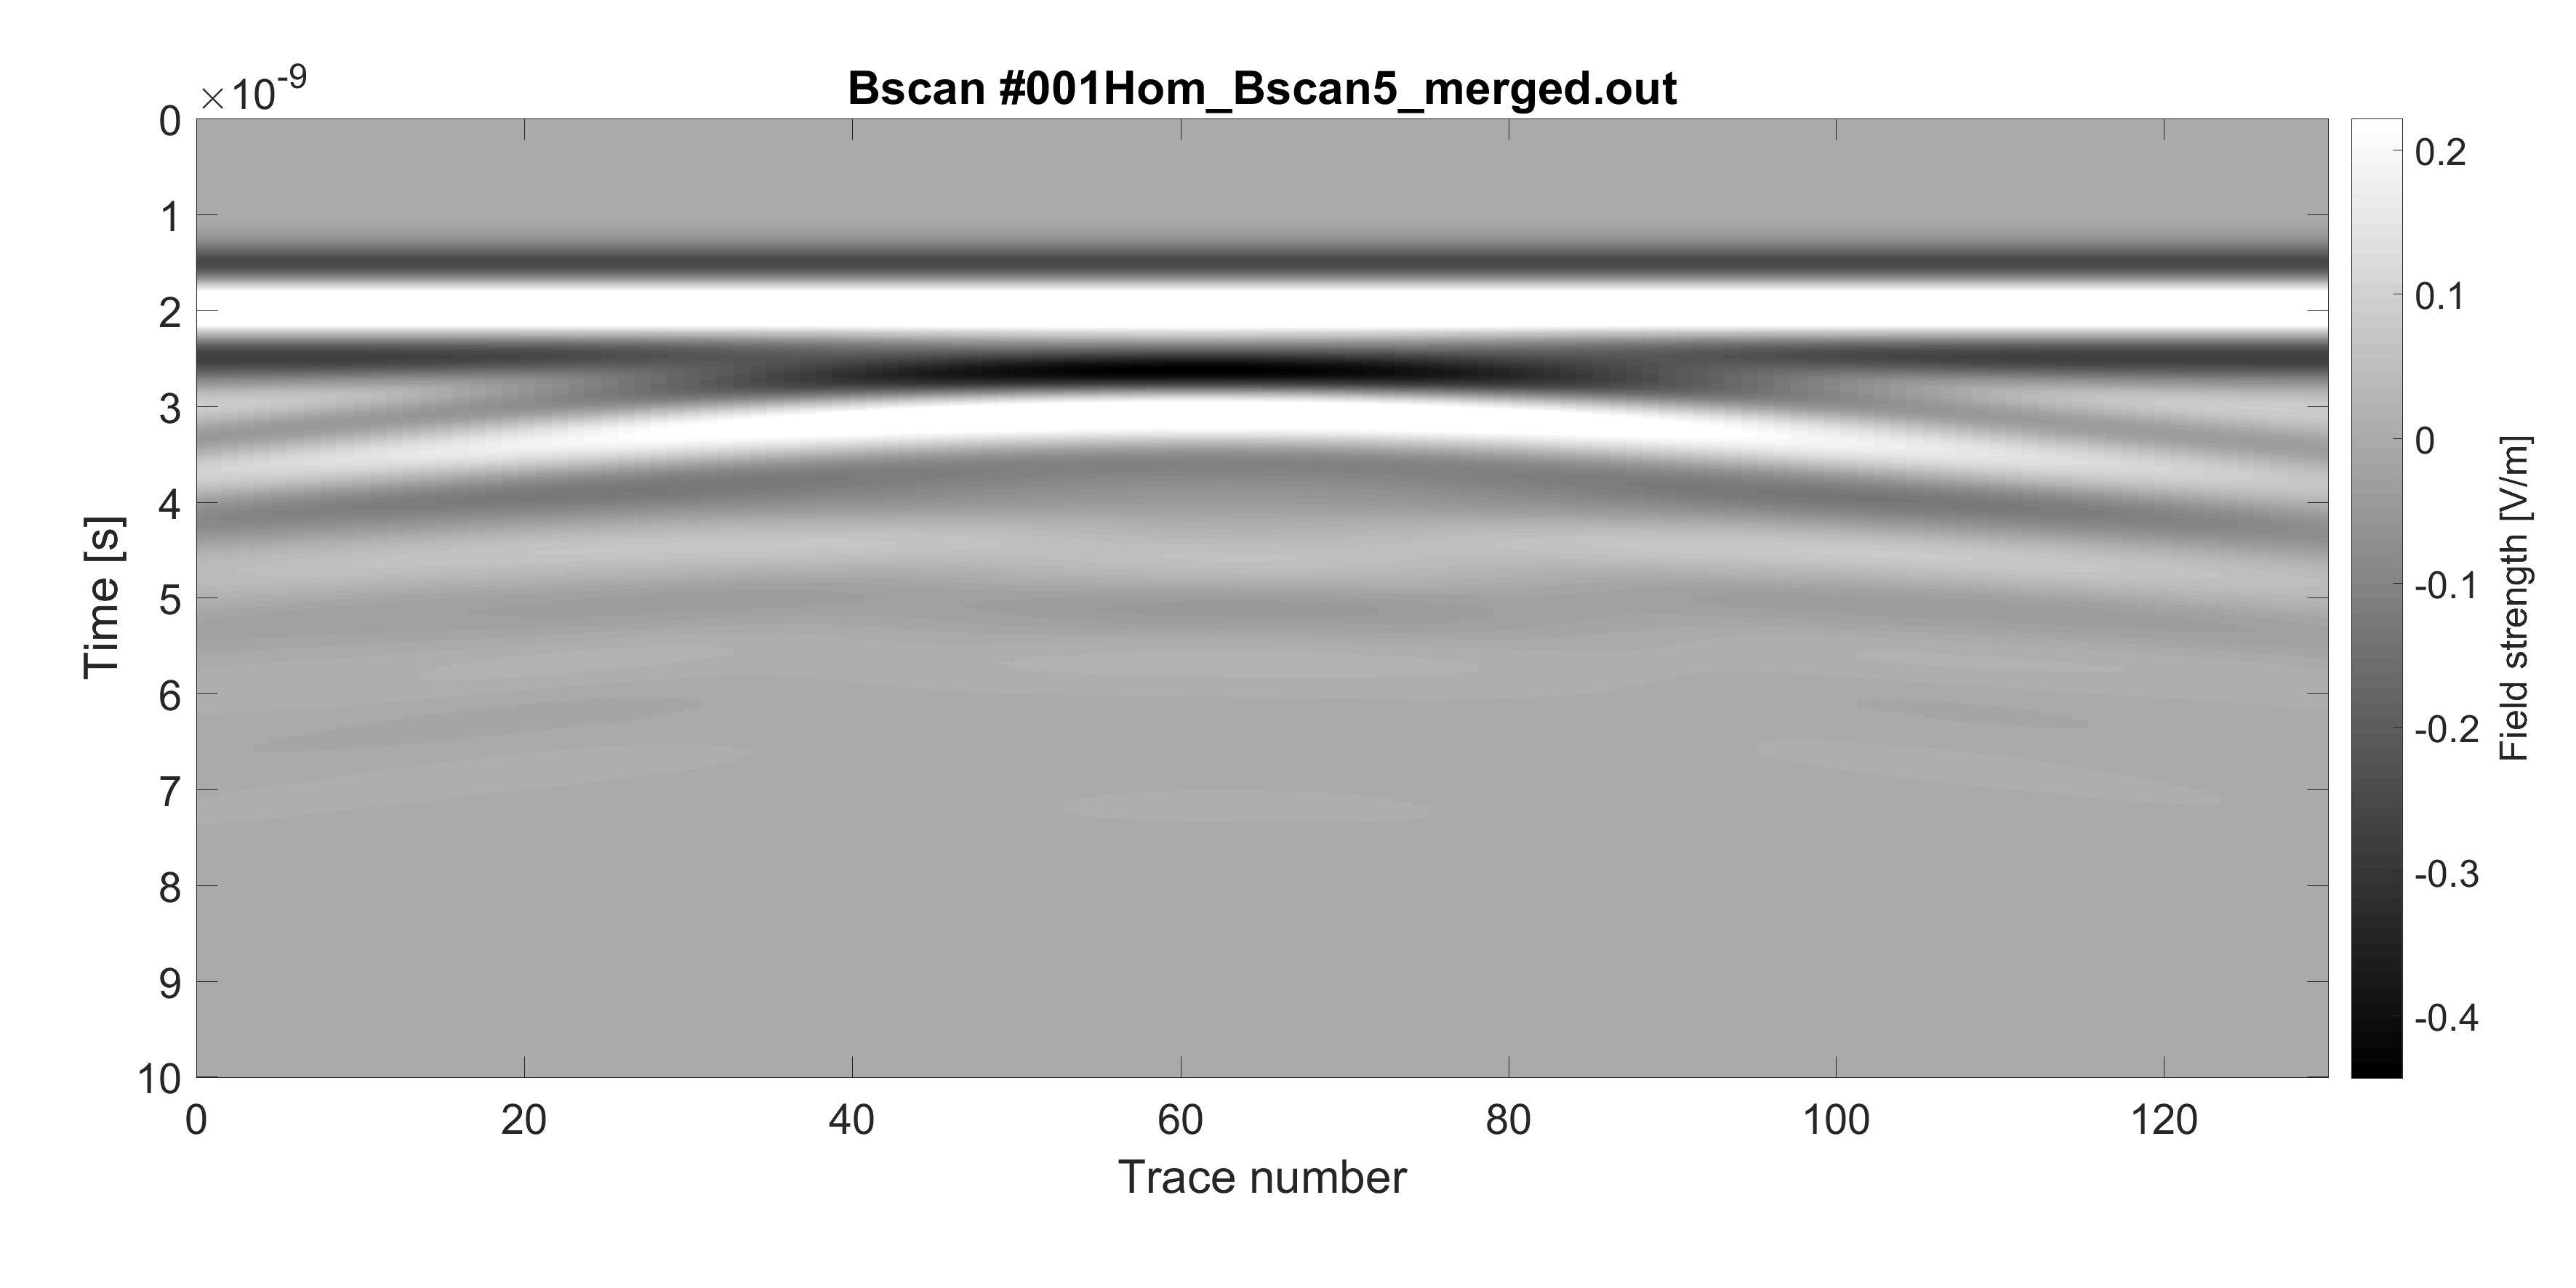
\includegraphics[width=0.47\textwidth, keepaspectratio,valign=c]{Homogeneo/001Hom_Bscan5_merged.png}}
\subfloat{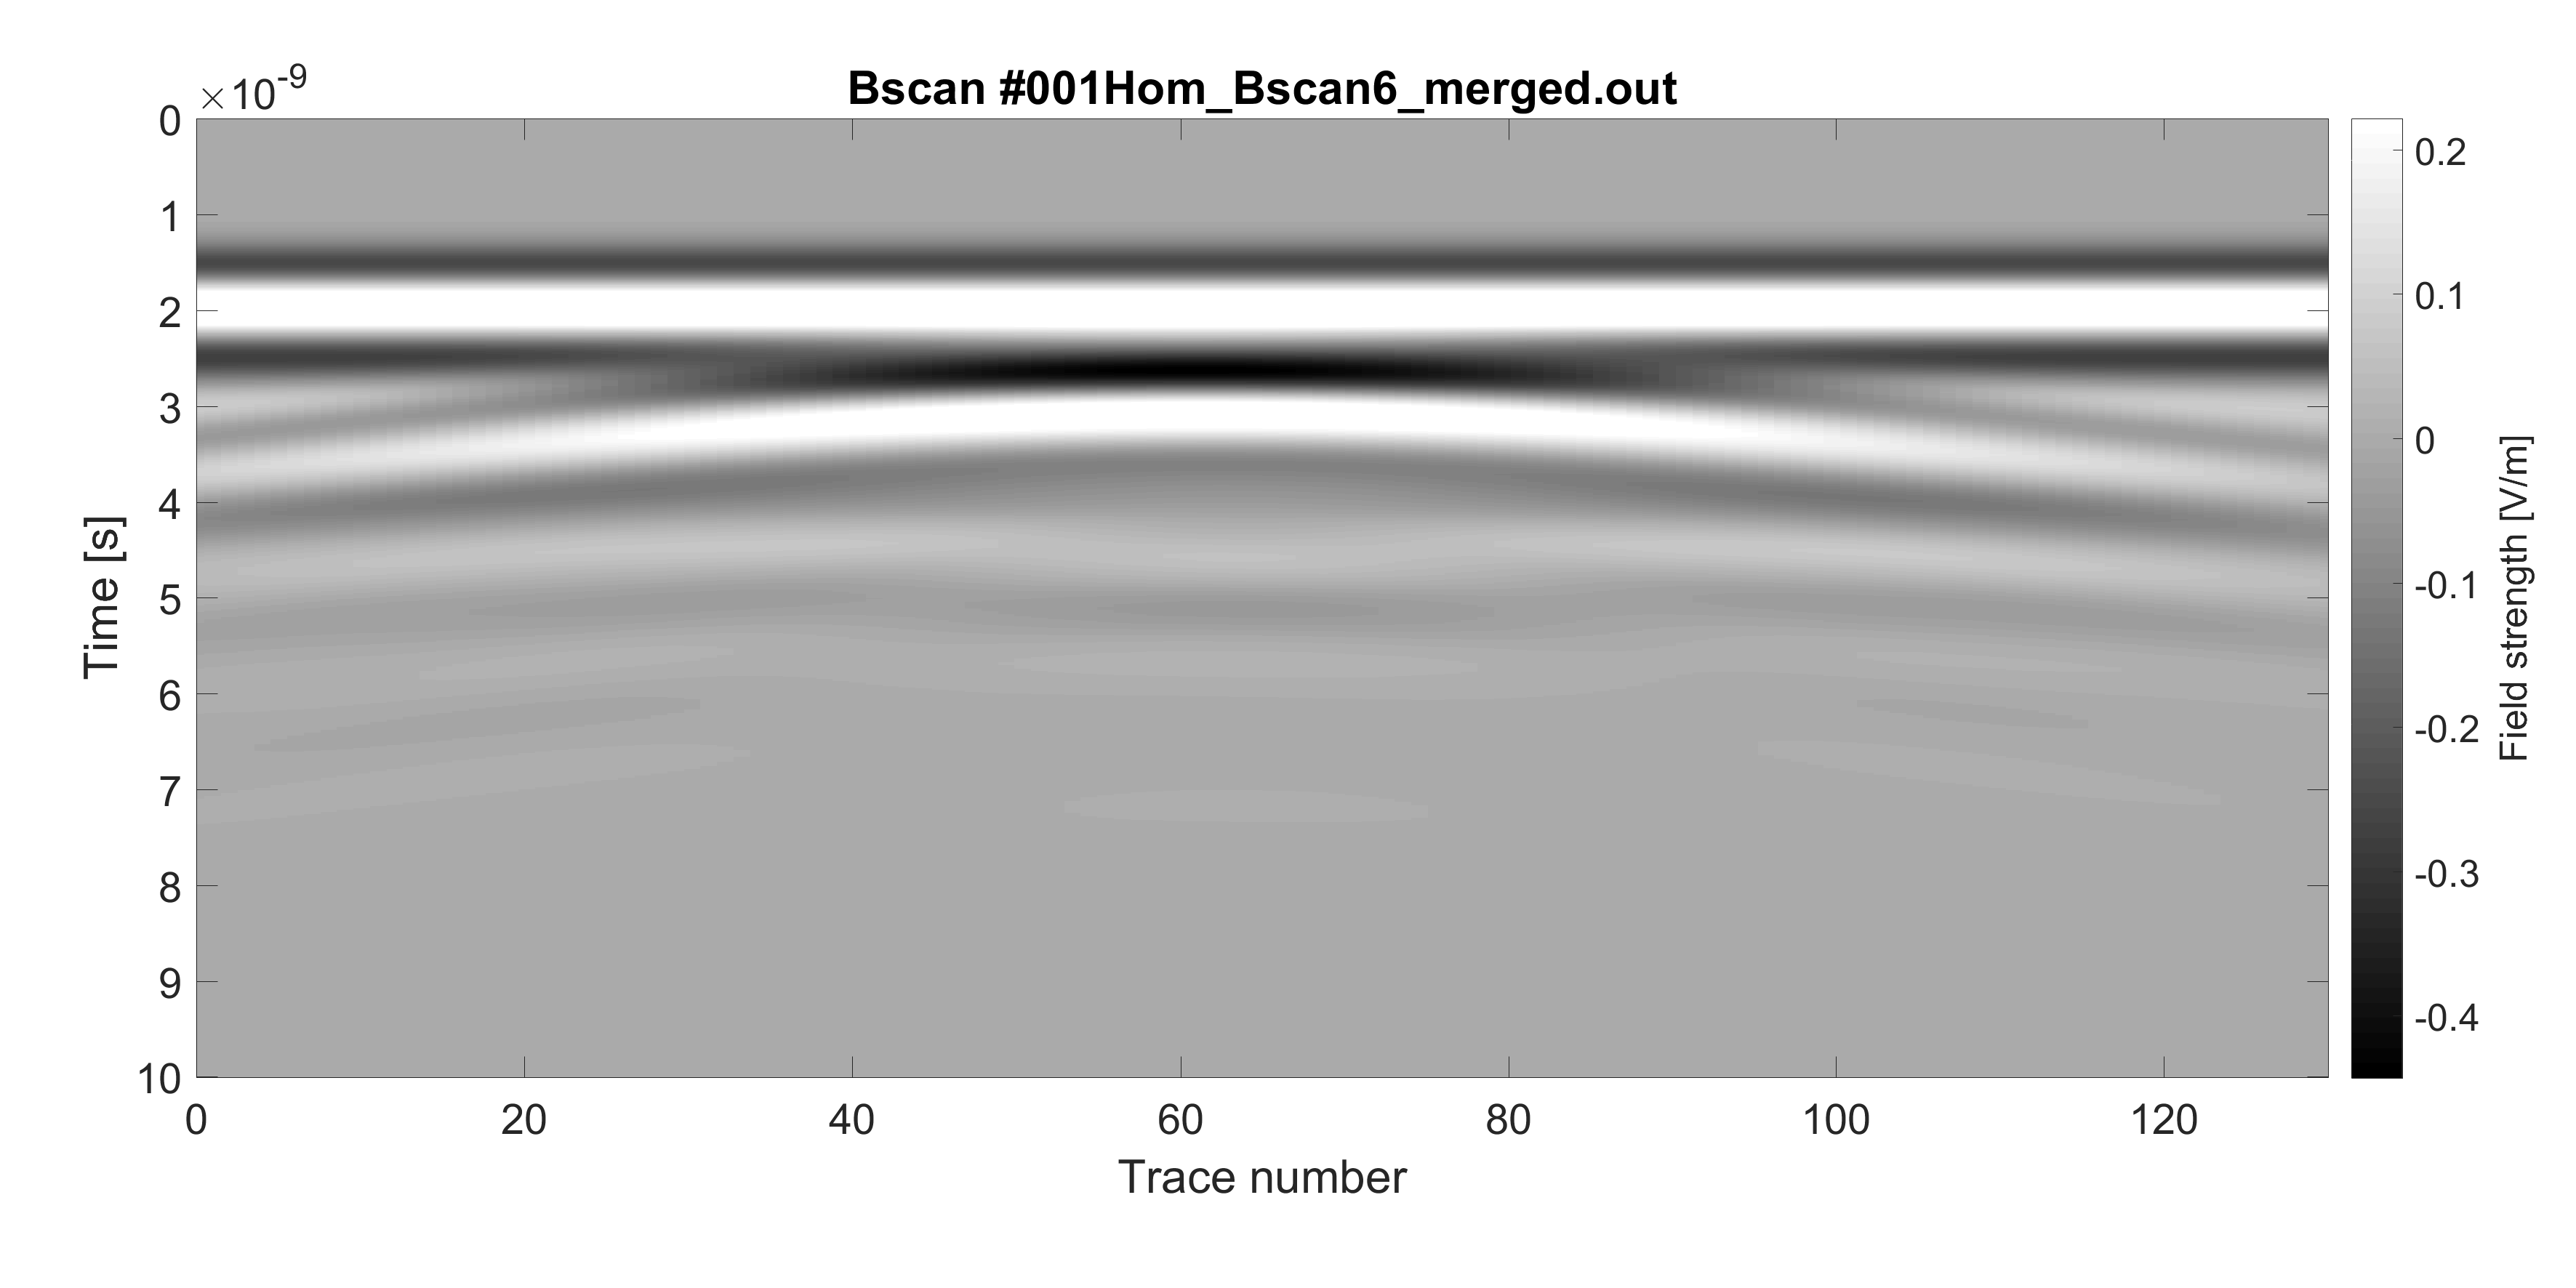
\includegraphics[width=0.47\textwidth, keepaspectratio,valign=c]{Homogeneo/001Hom_Bscan6_merged.png}} 
\subfloat{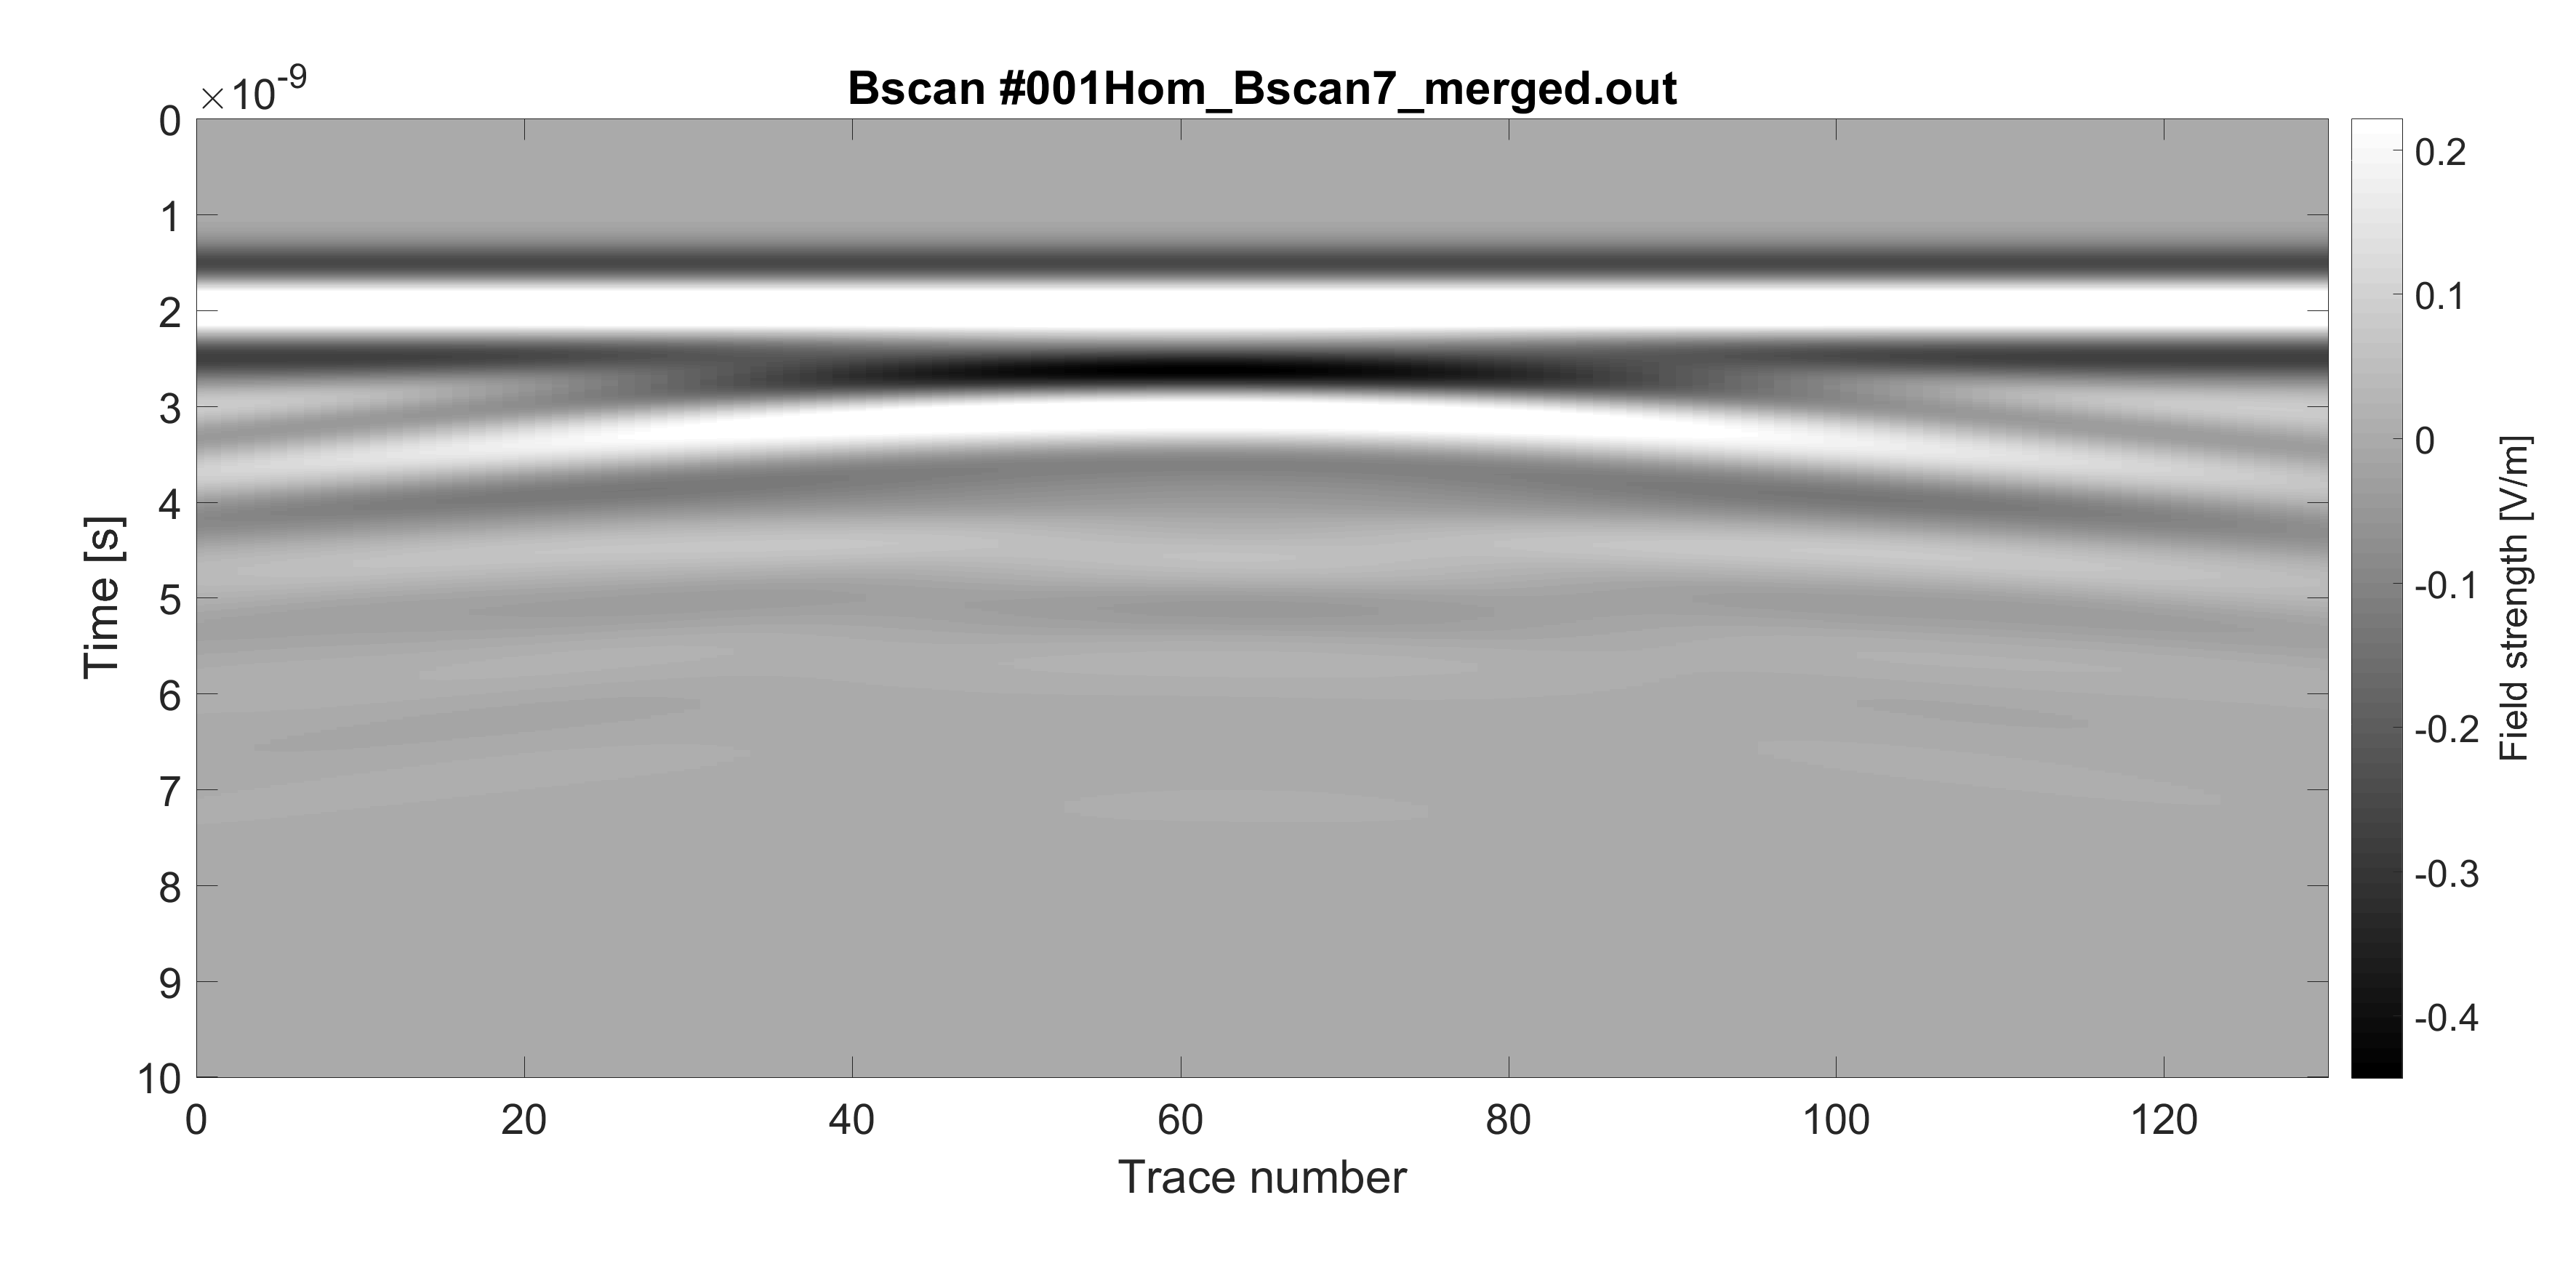
\includegraphics[width=0.47\textwidth, keepaspectratio,valign=c]{Homogeneo/001Hom_Bscan7_merged.png}}
\subfloat{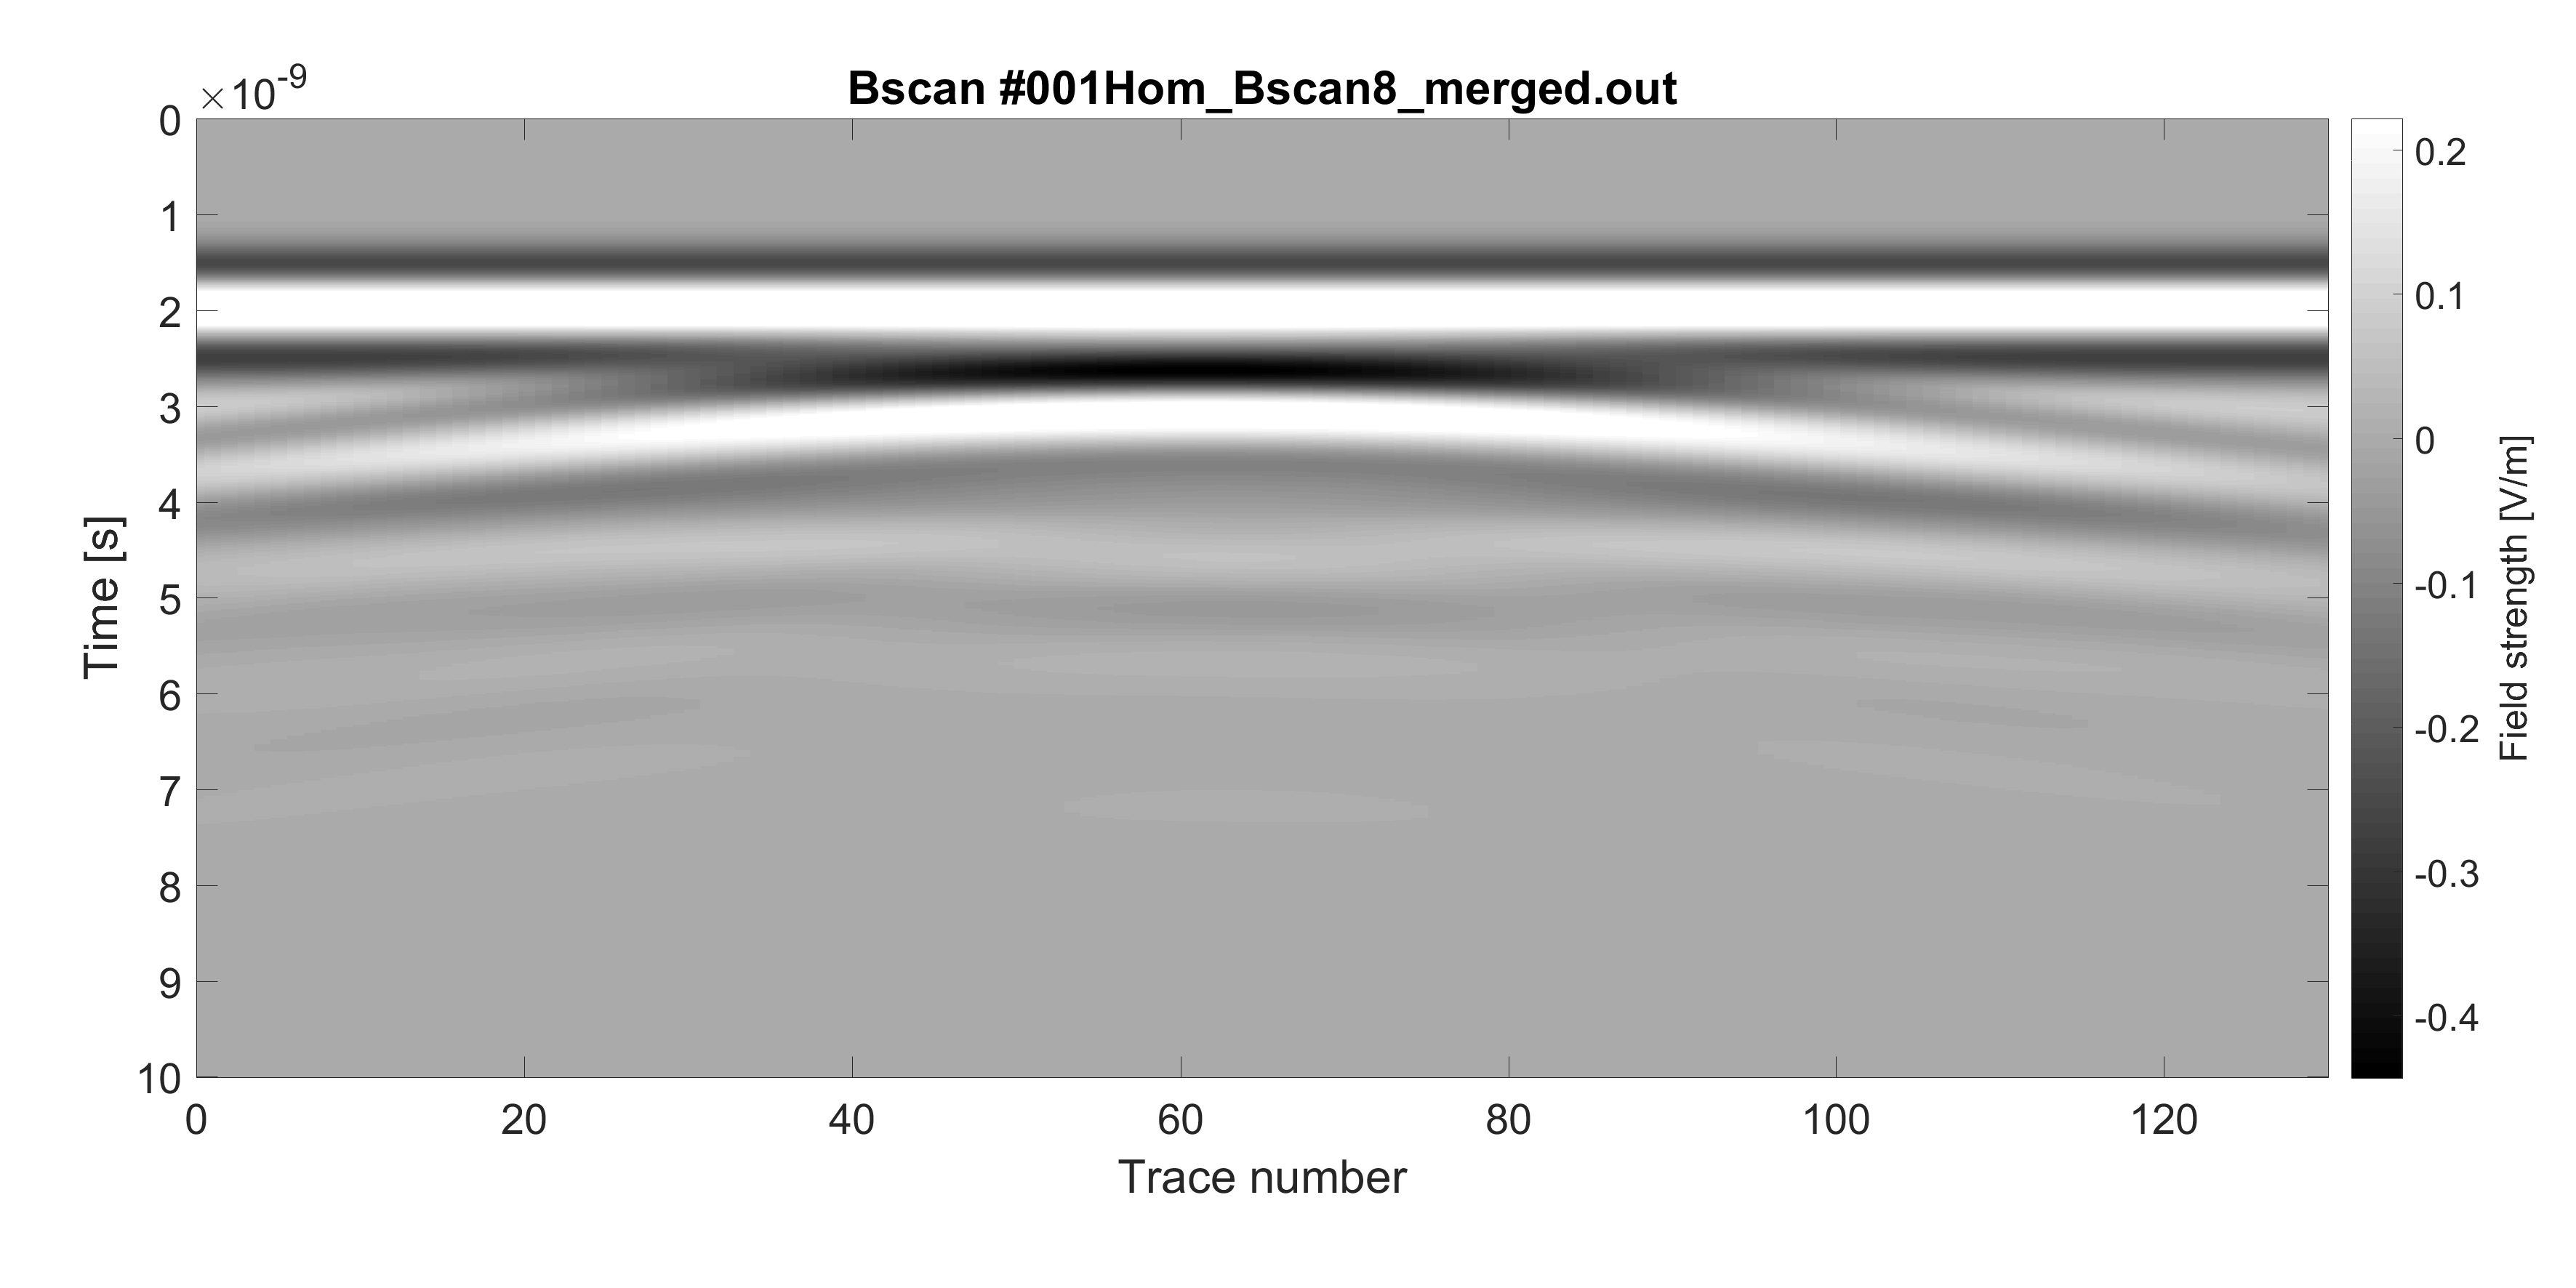
\includegraphics[width=0.47\textwidth, keepaspectratio,valign=c]{Homogeneo/001Hom_Bscan8_merged.png}}
\subfloat{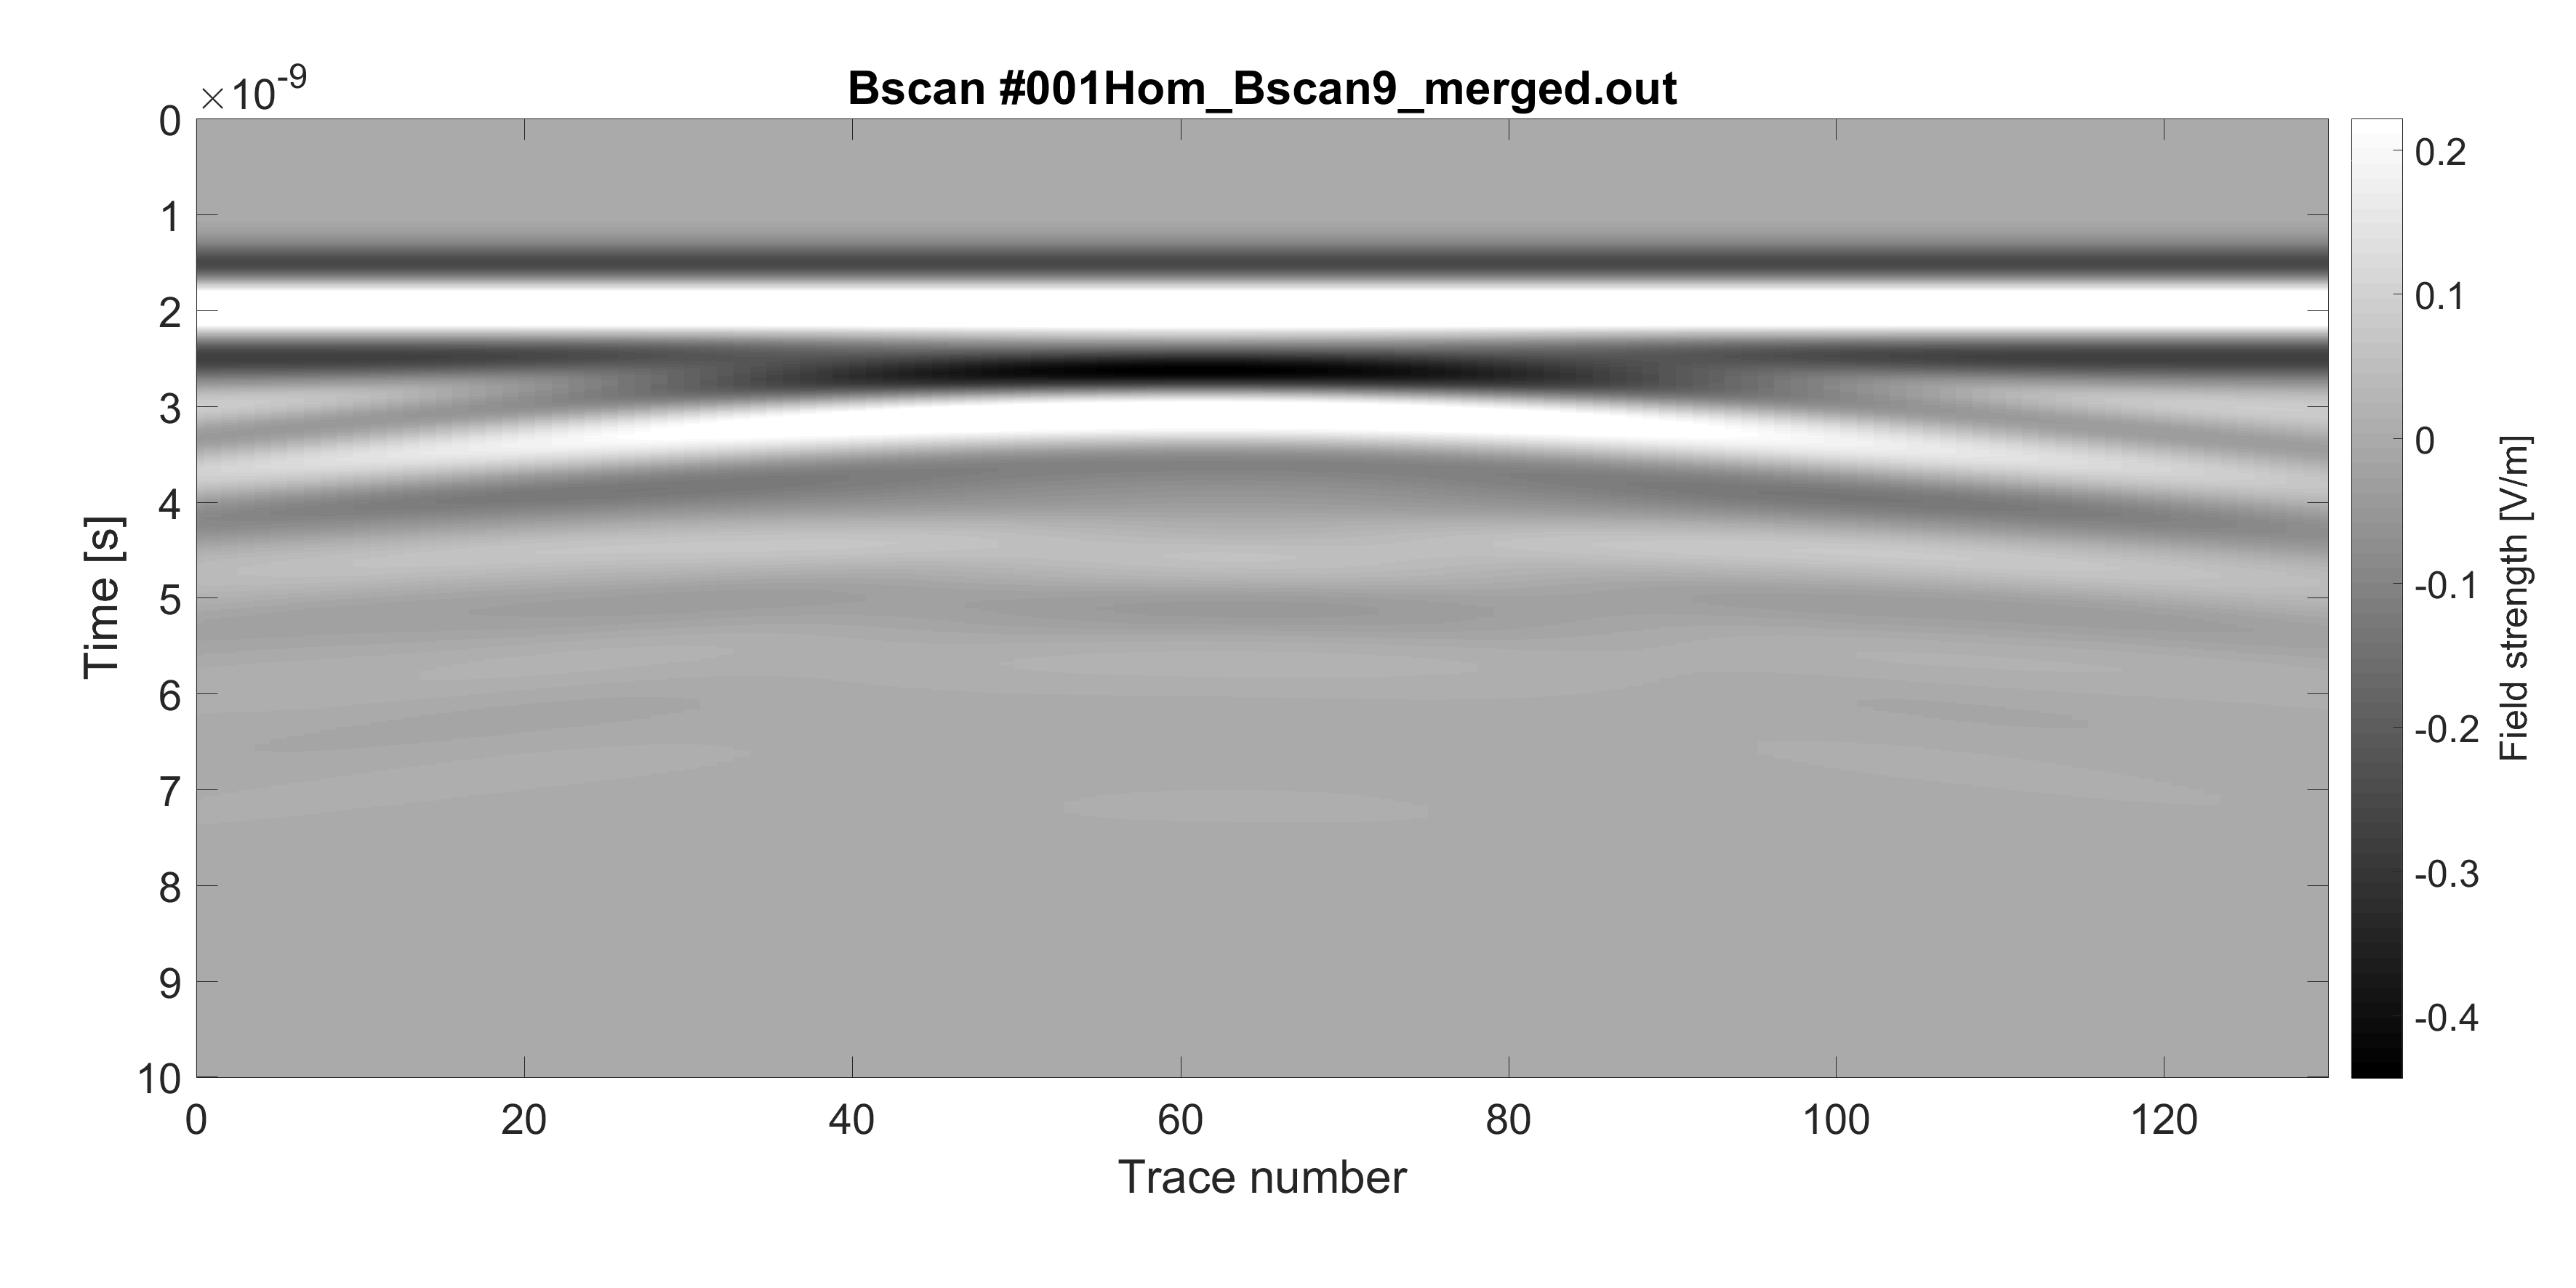
\includegraphics[width=0.47\textwidth, keepaspectratio,valign=c]{Homogeneo/001Hom_Bscan9_merged.png}}
\subfloat{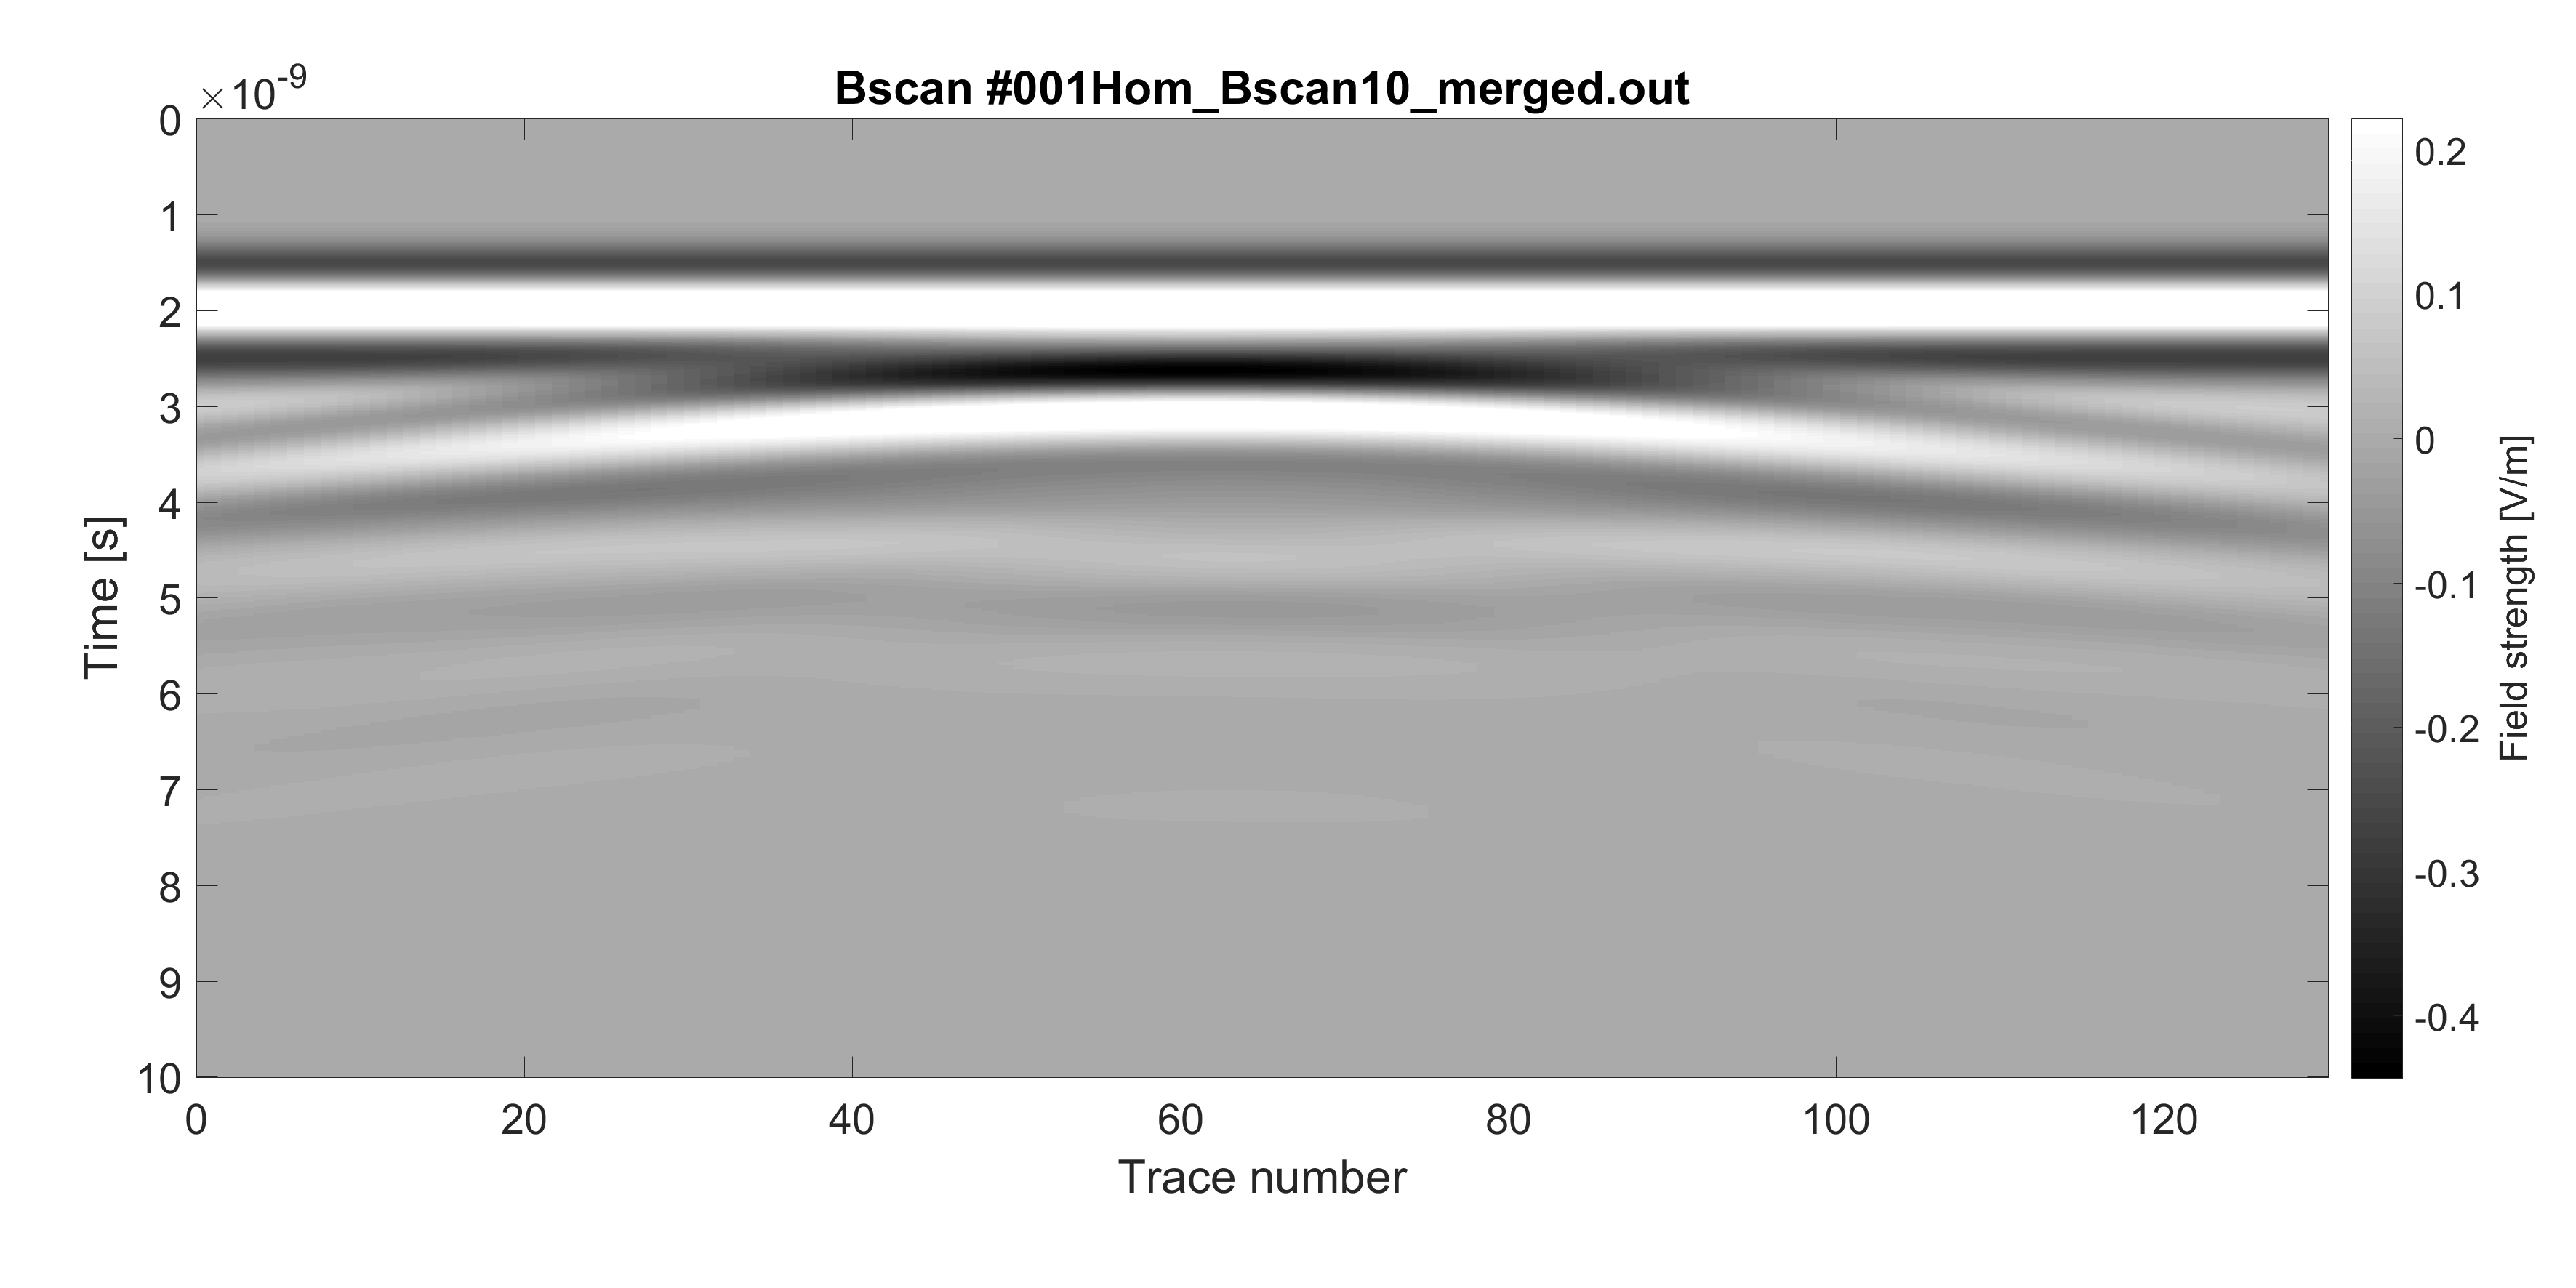
\includegraphics[width=0.47\textwidth, keepaspectratio,valign=c]{Homogeneo/001Hom_Bscan10_merged.png}} 
\subfloat{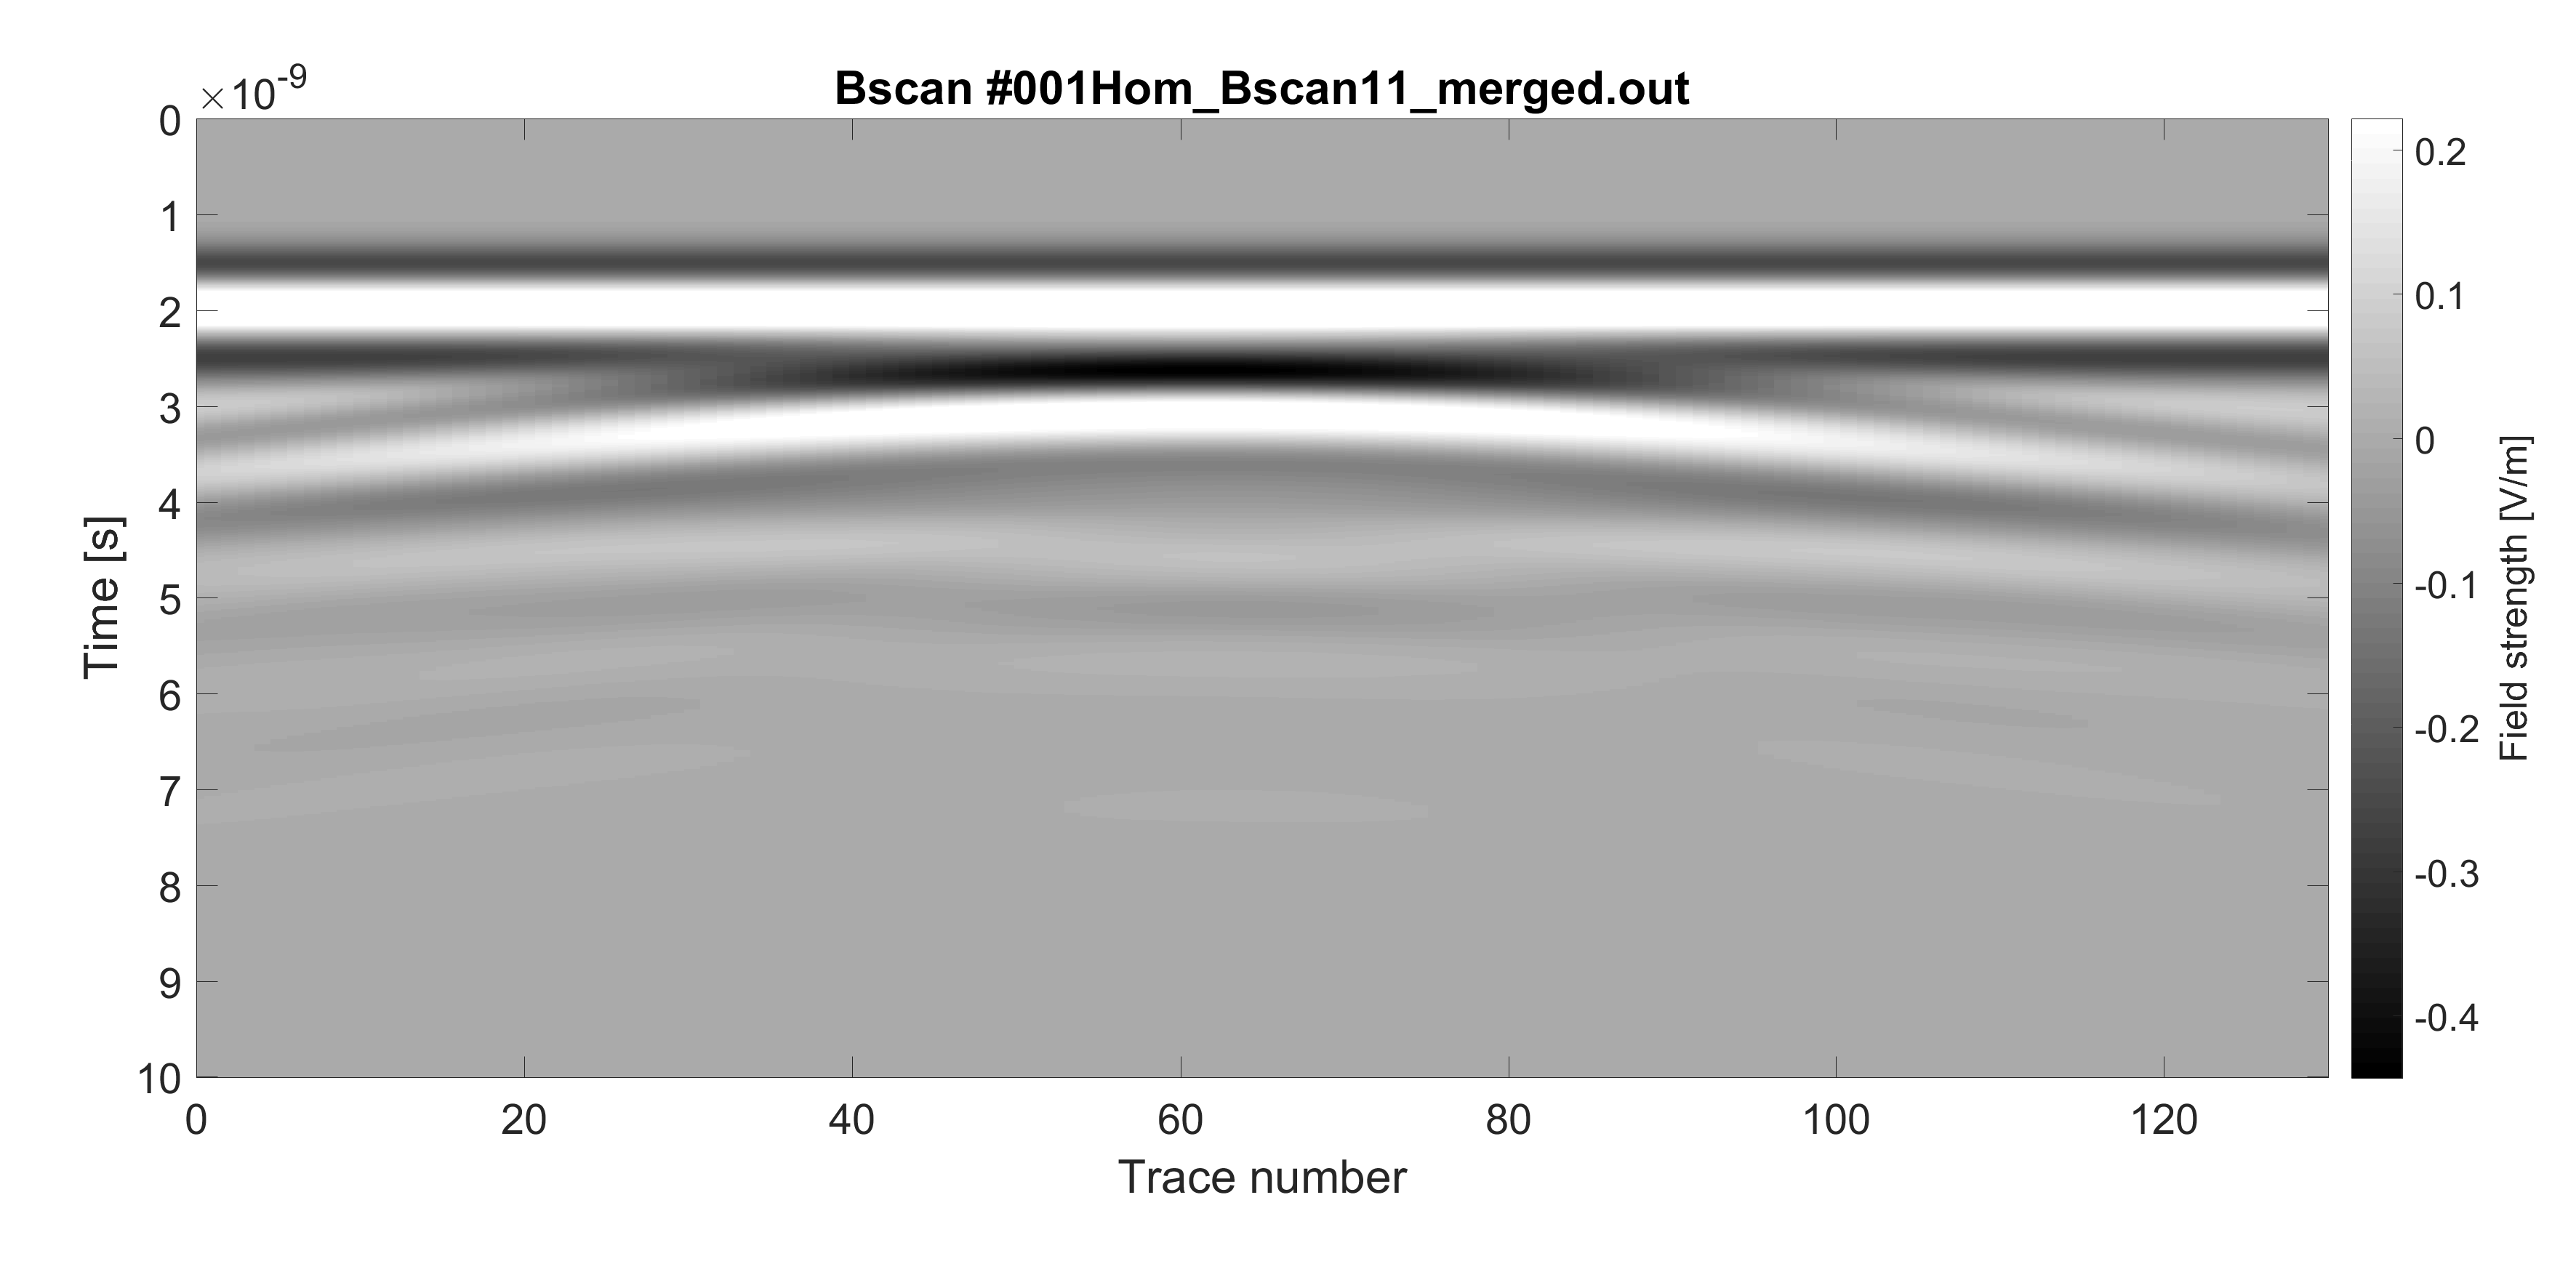
\includegraphics[width=0.47\textwidth, keepaspectratio,valign=c]{Homogeneo/001Hom_Bscan11_merged.png}}
\subfloat{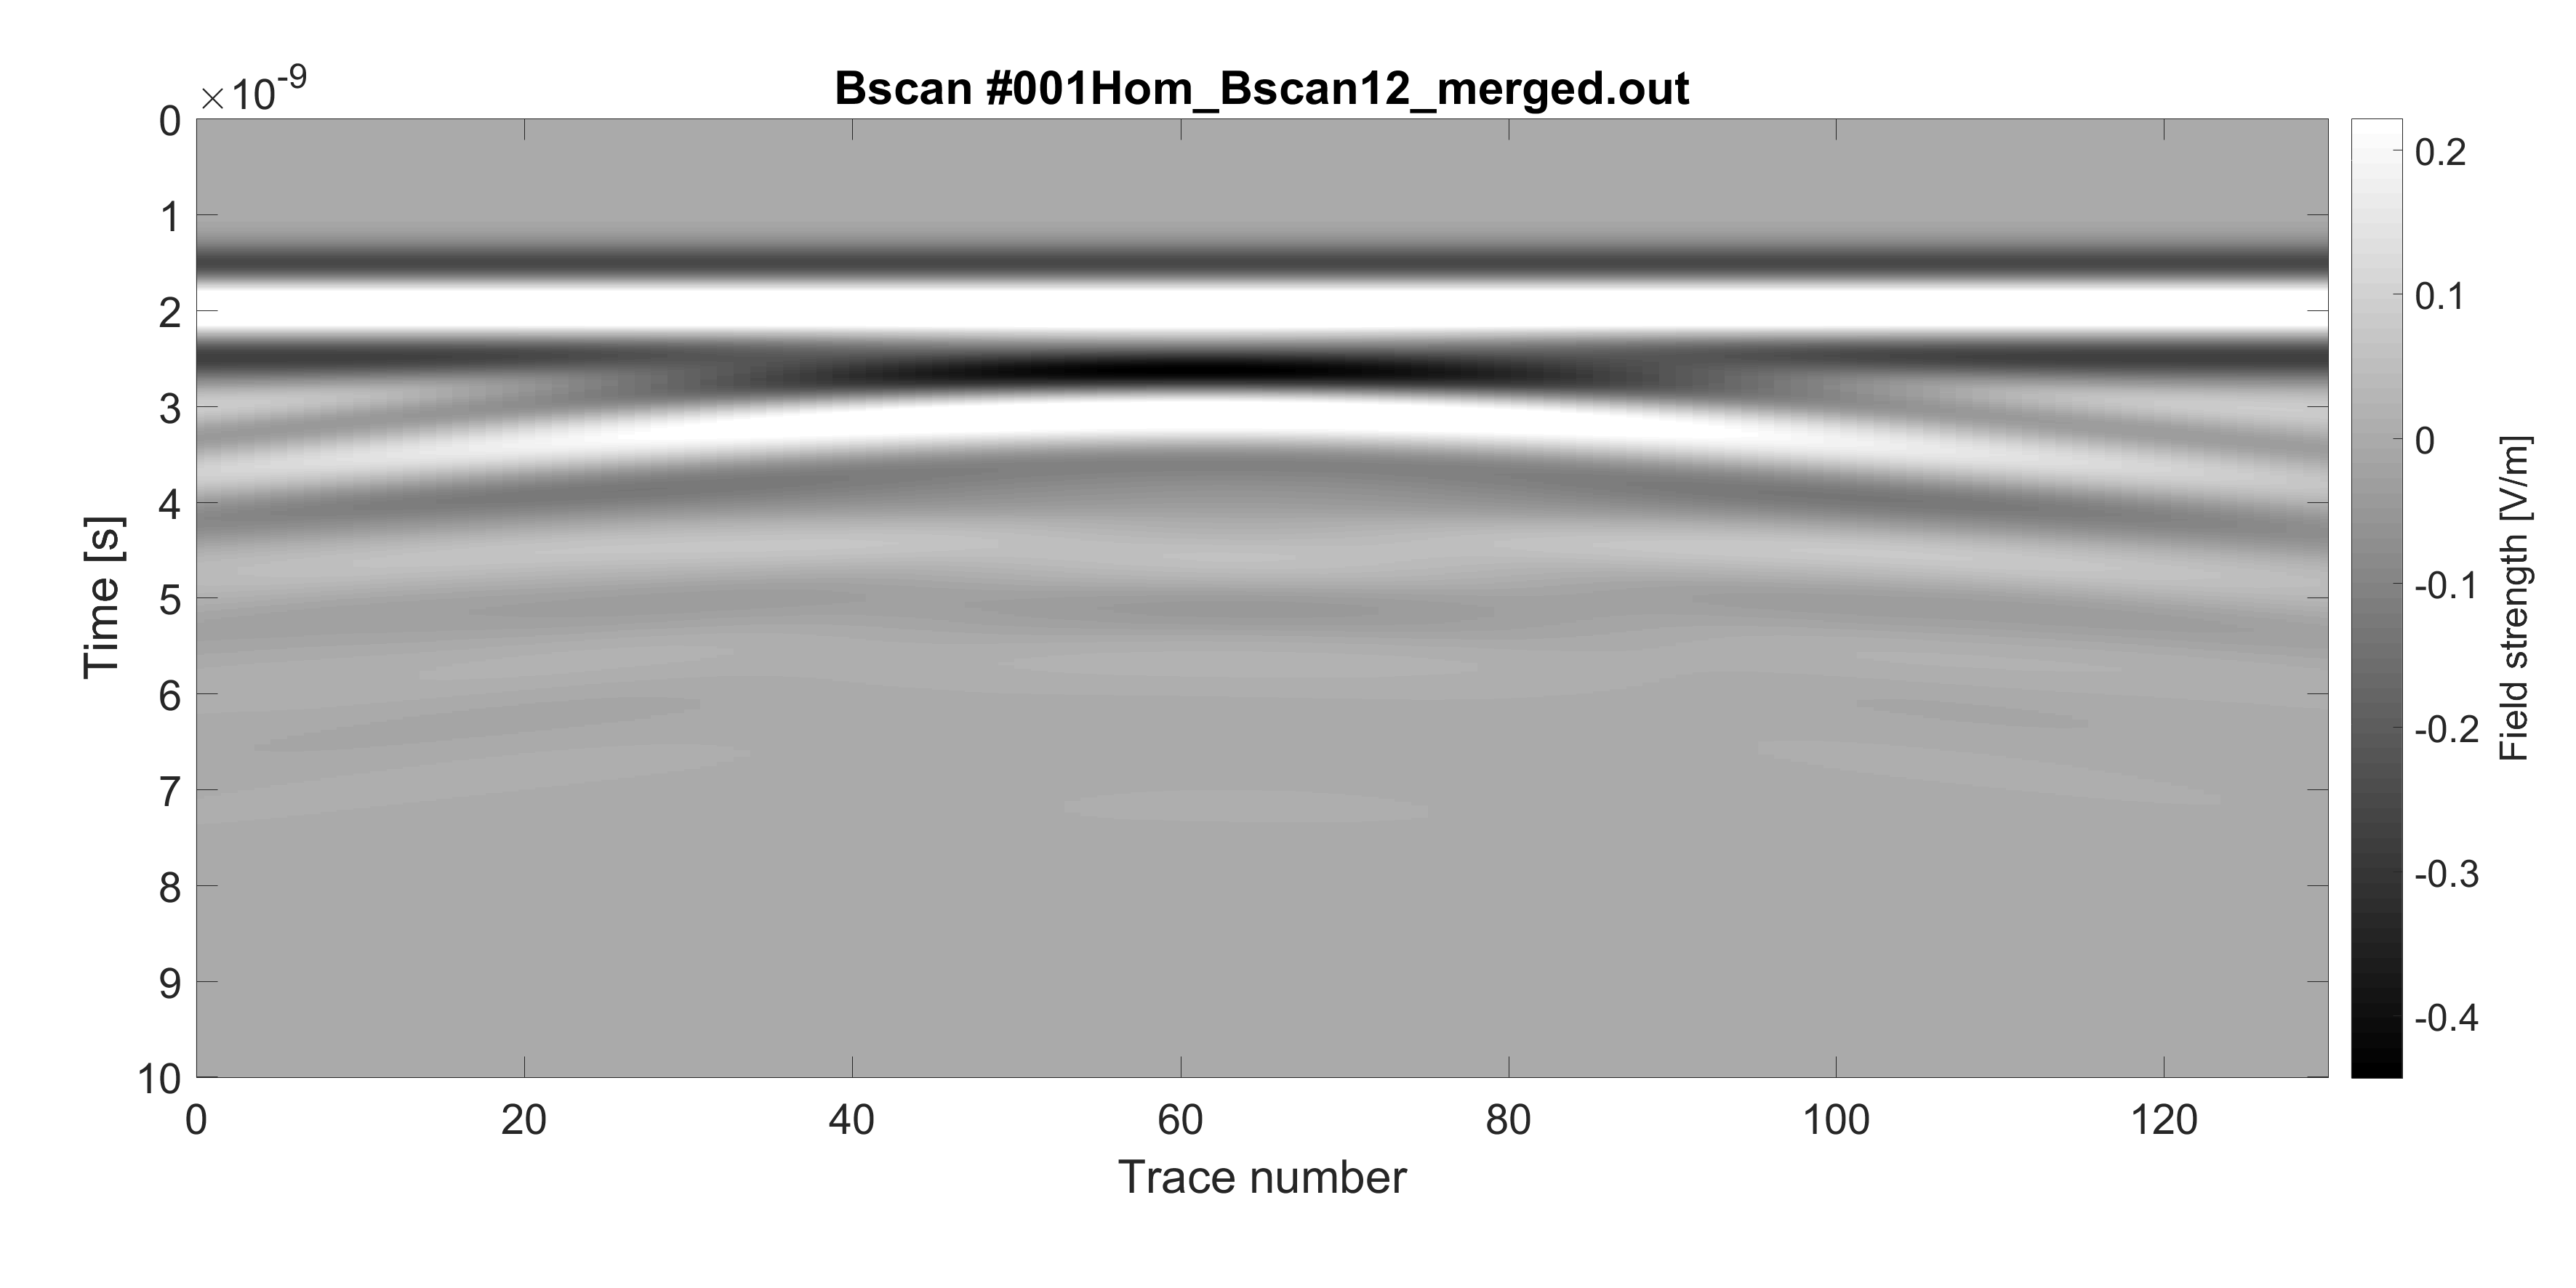
\includegraphics[width=0.47\textwidth, keepaspectratio,valign=c]{Homogeneo/001Hom_Bscan12_merged.png}}
\subfloat{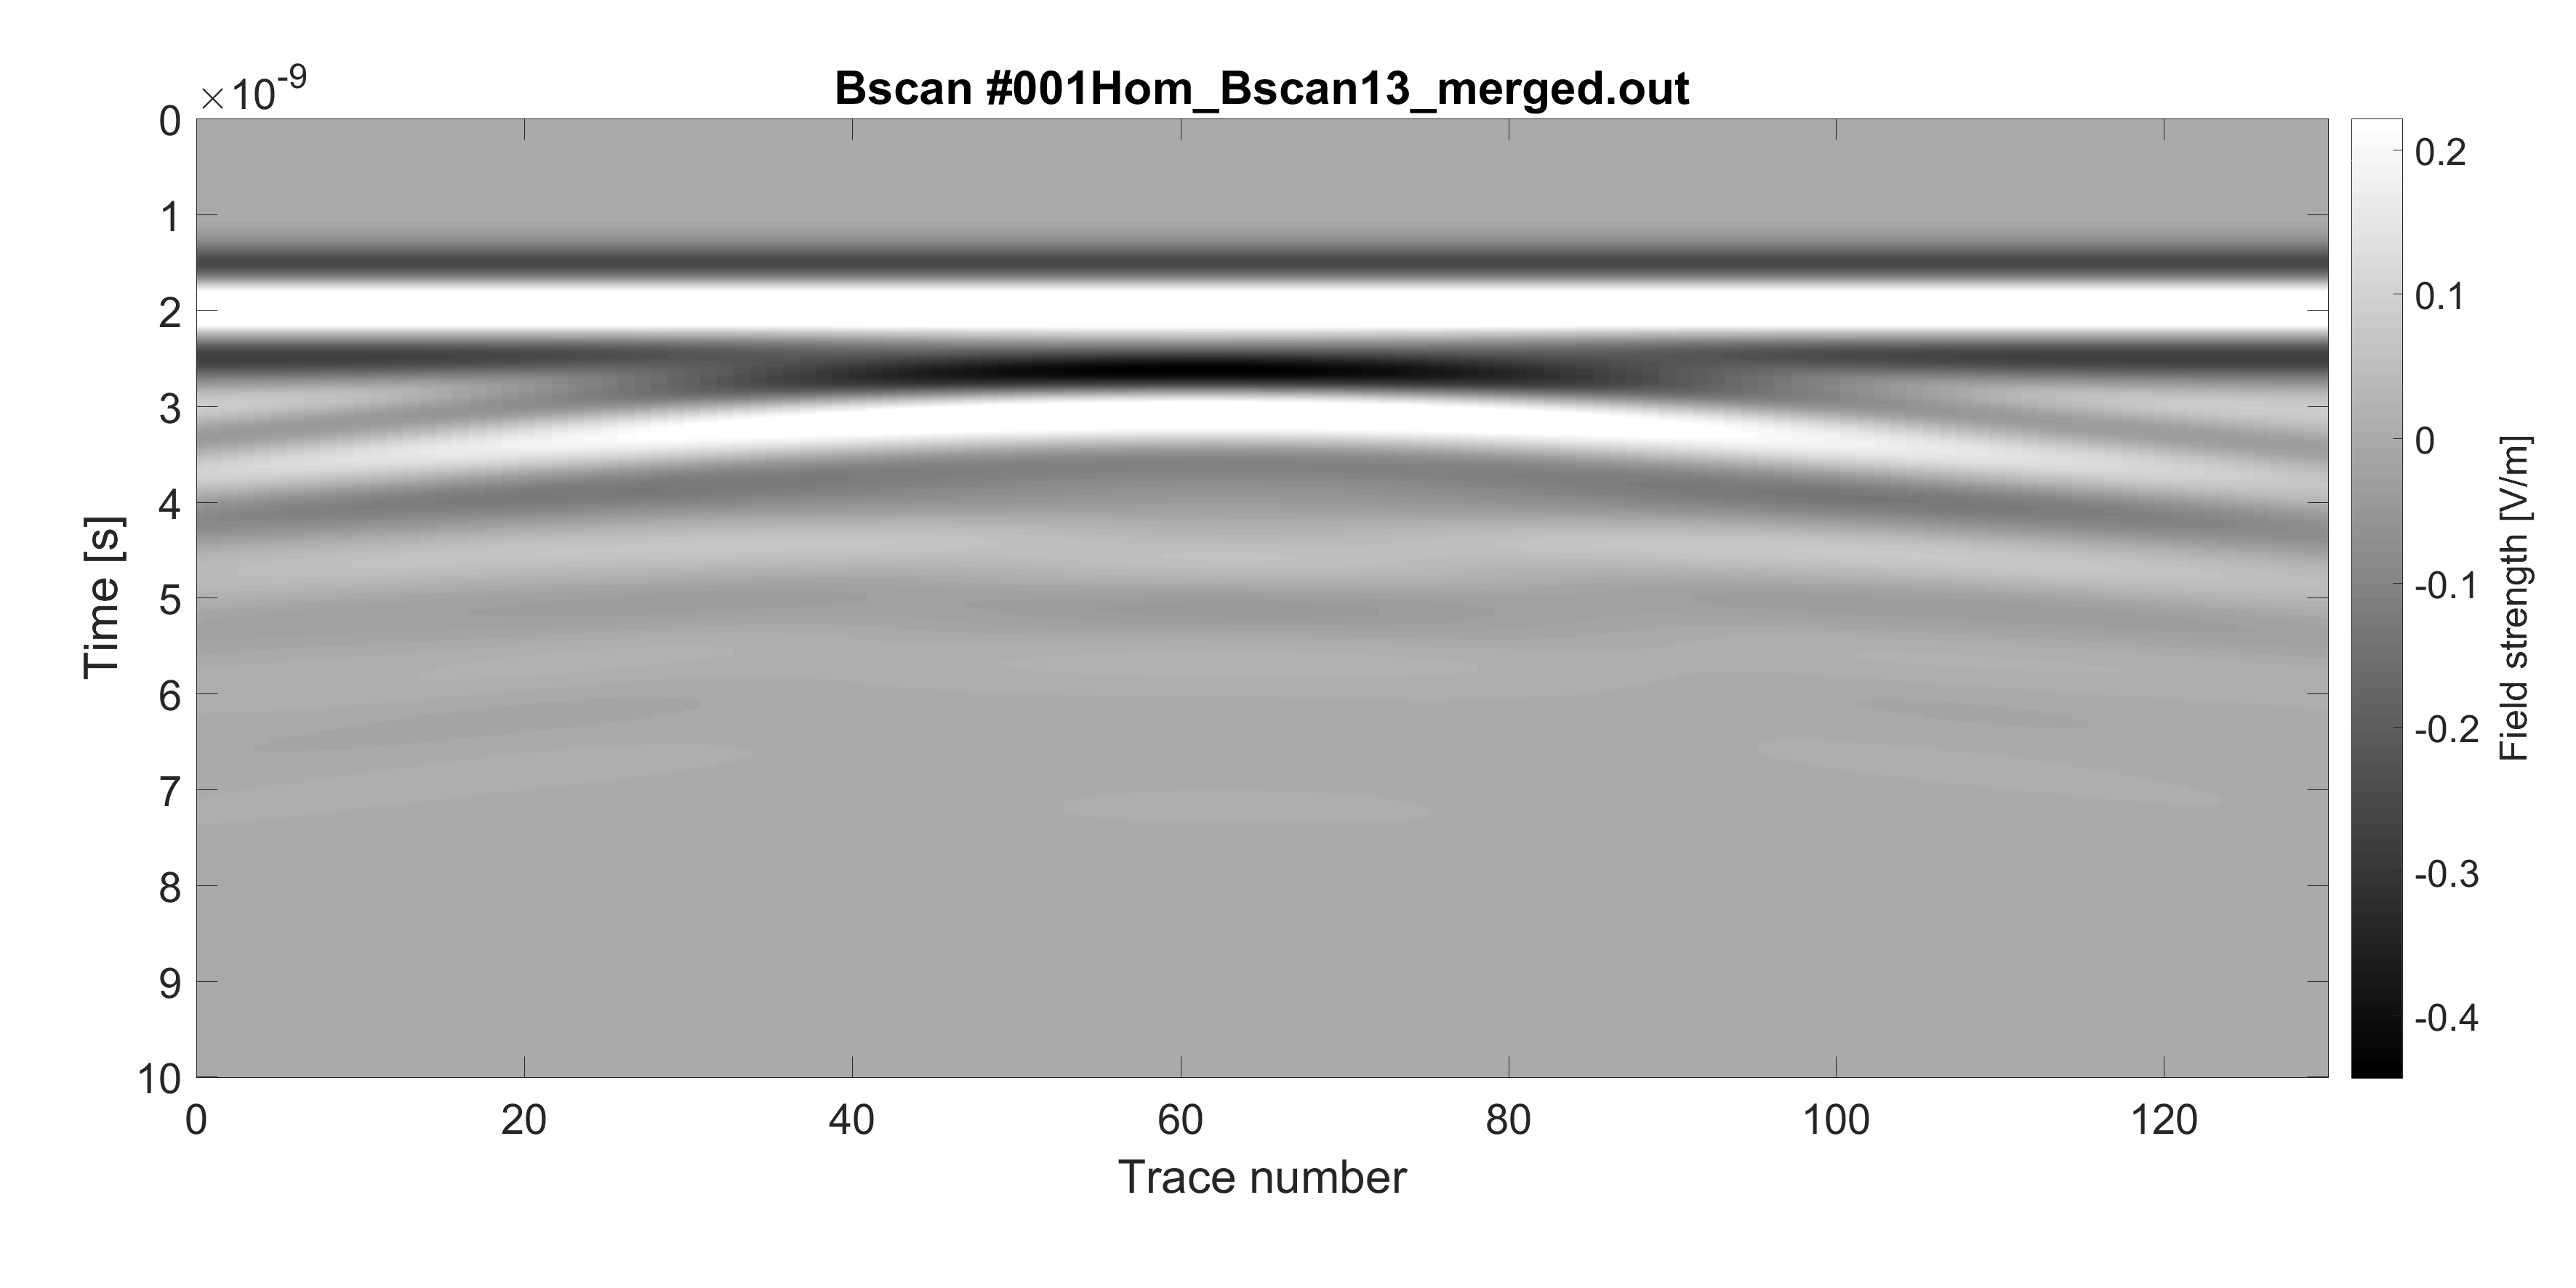
\includegraphics[width=0.47\textwidth, keepaspectratio,valign=c]{Homogeneo/001Hom_Bscan13_merged.png}}
\subfloat{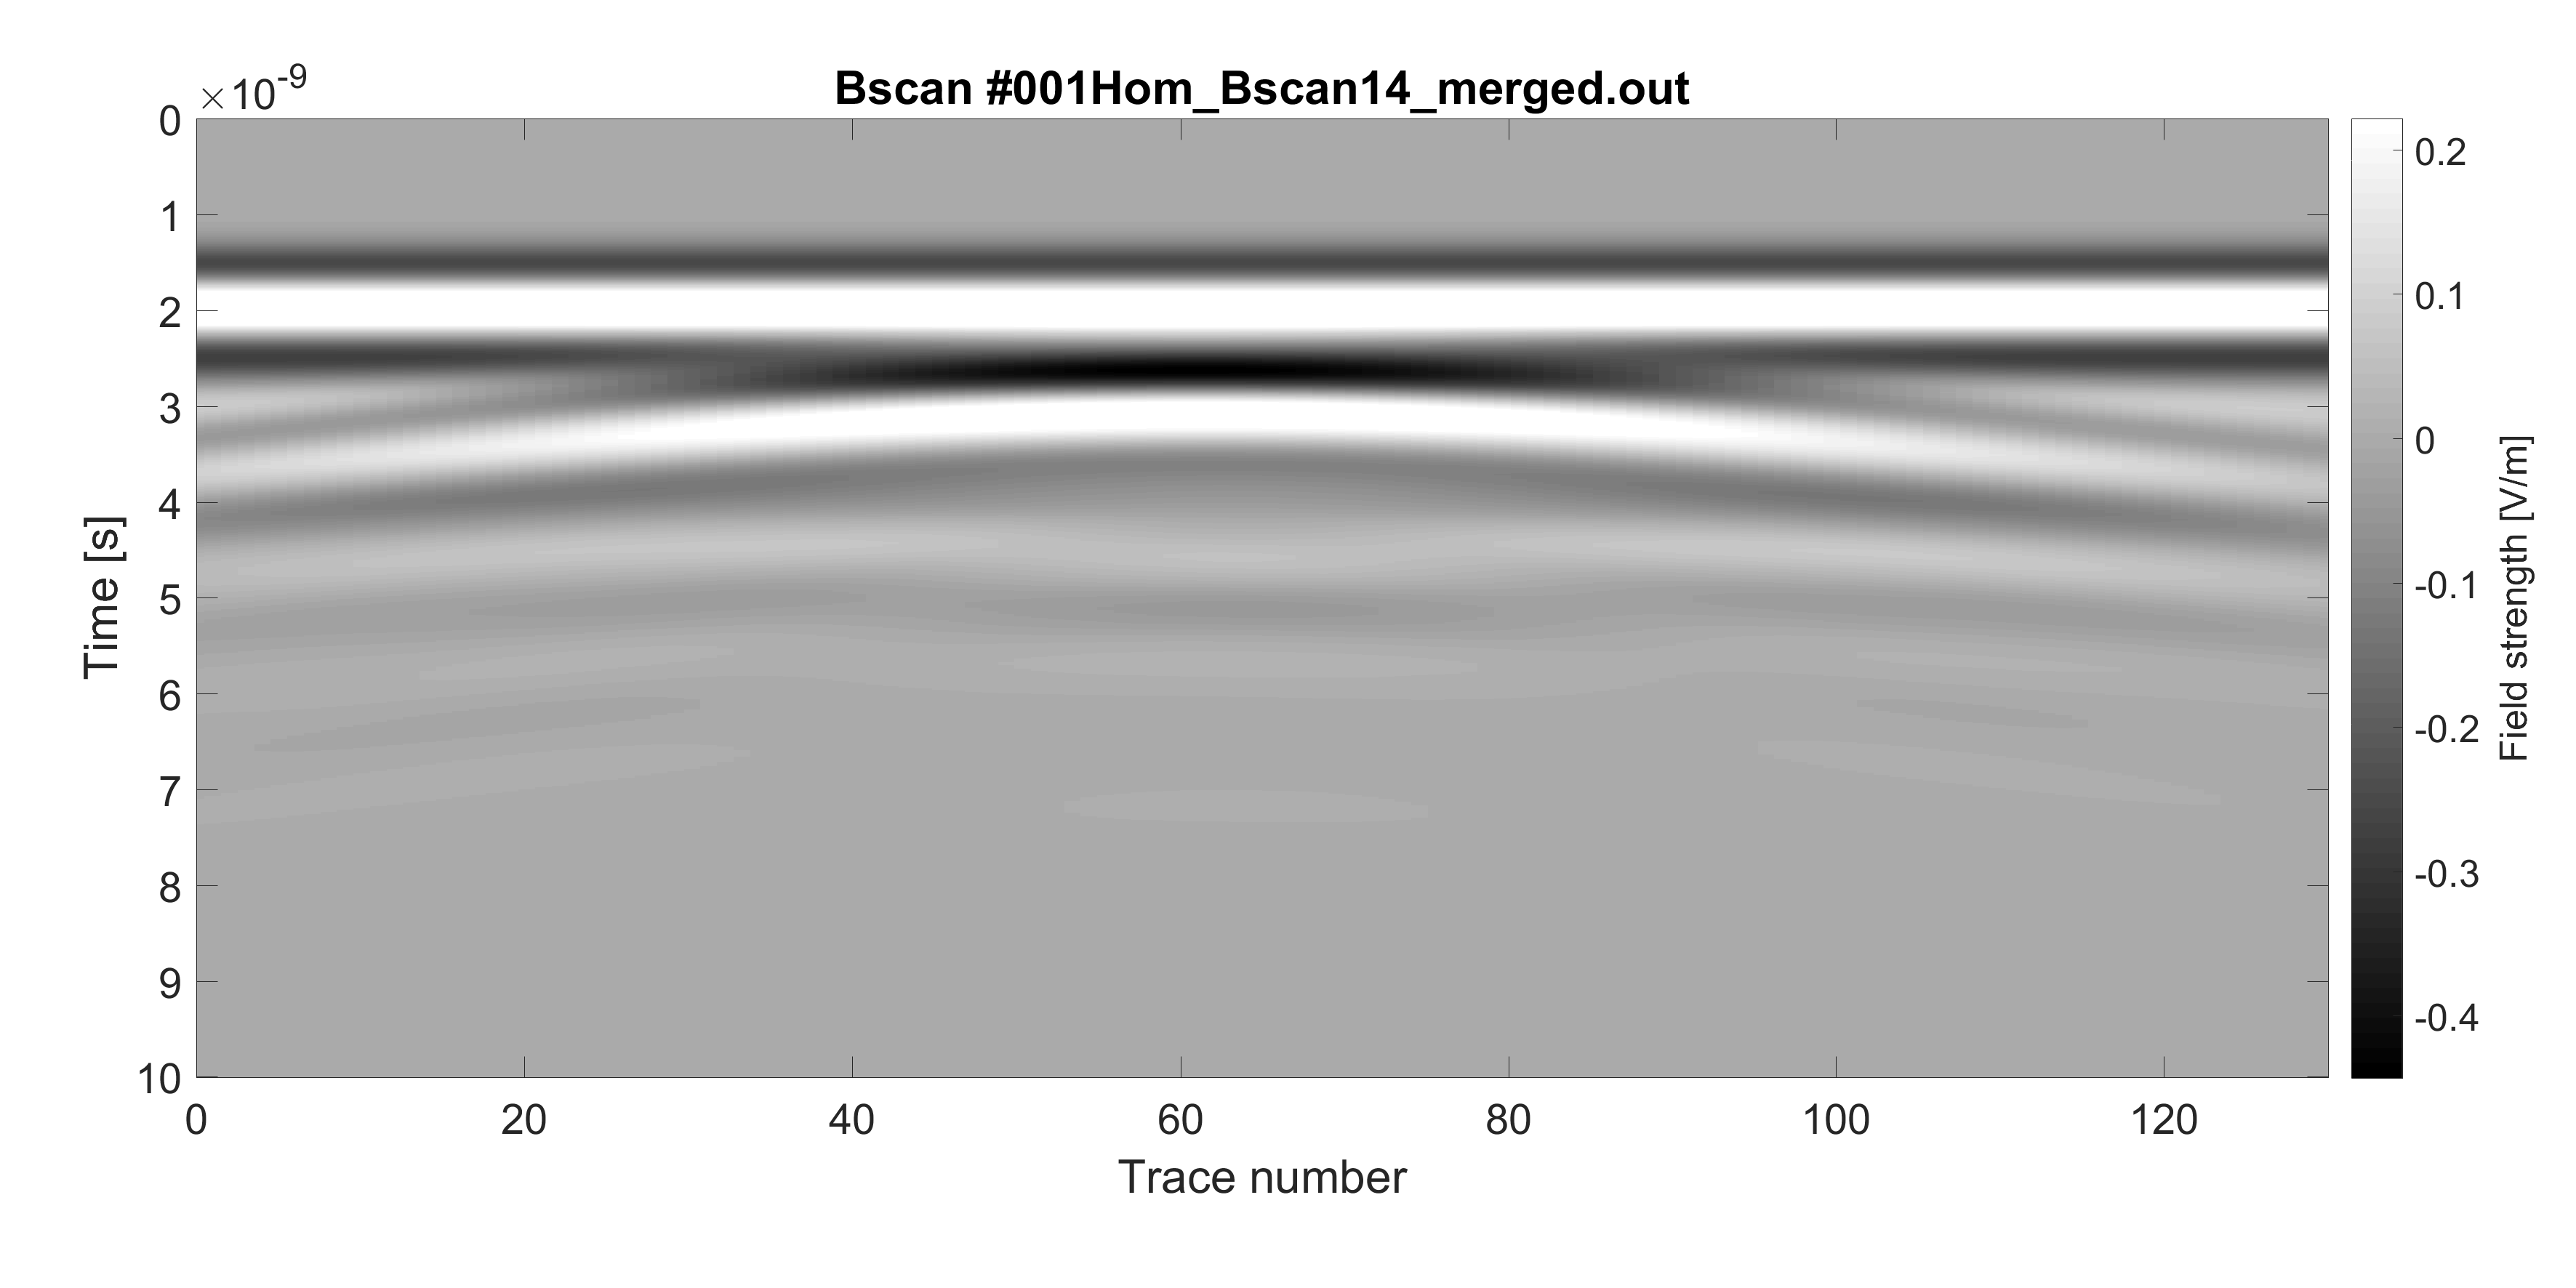
\includegraphics[width=0.47\textwidth, keepaspectratio,valign=c]{Homogeneo/001Hom_Bscan14_merged.png}}
\subfloat{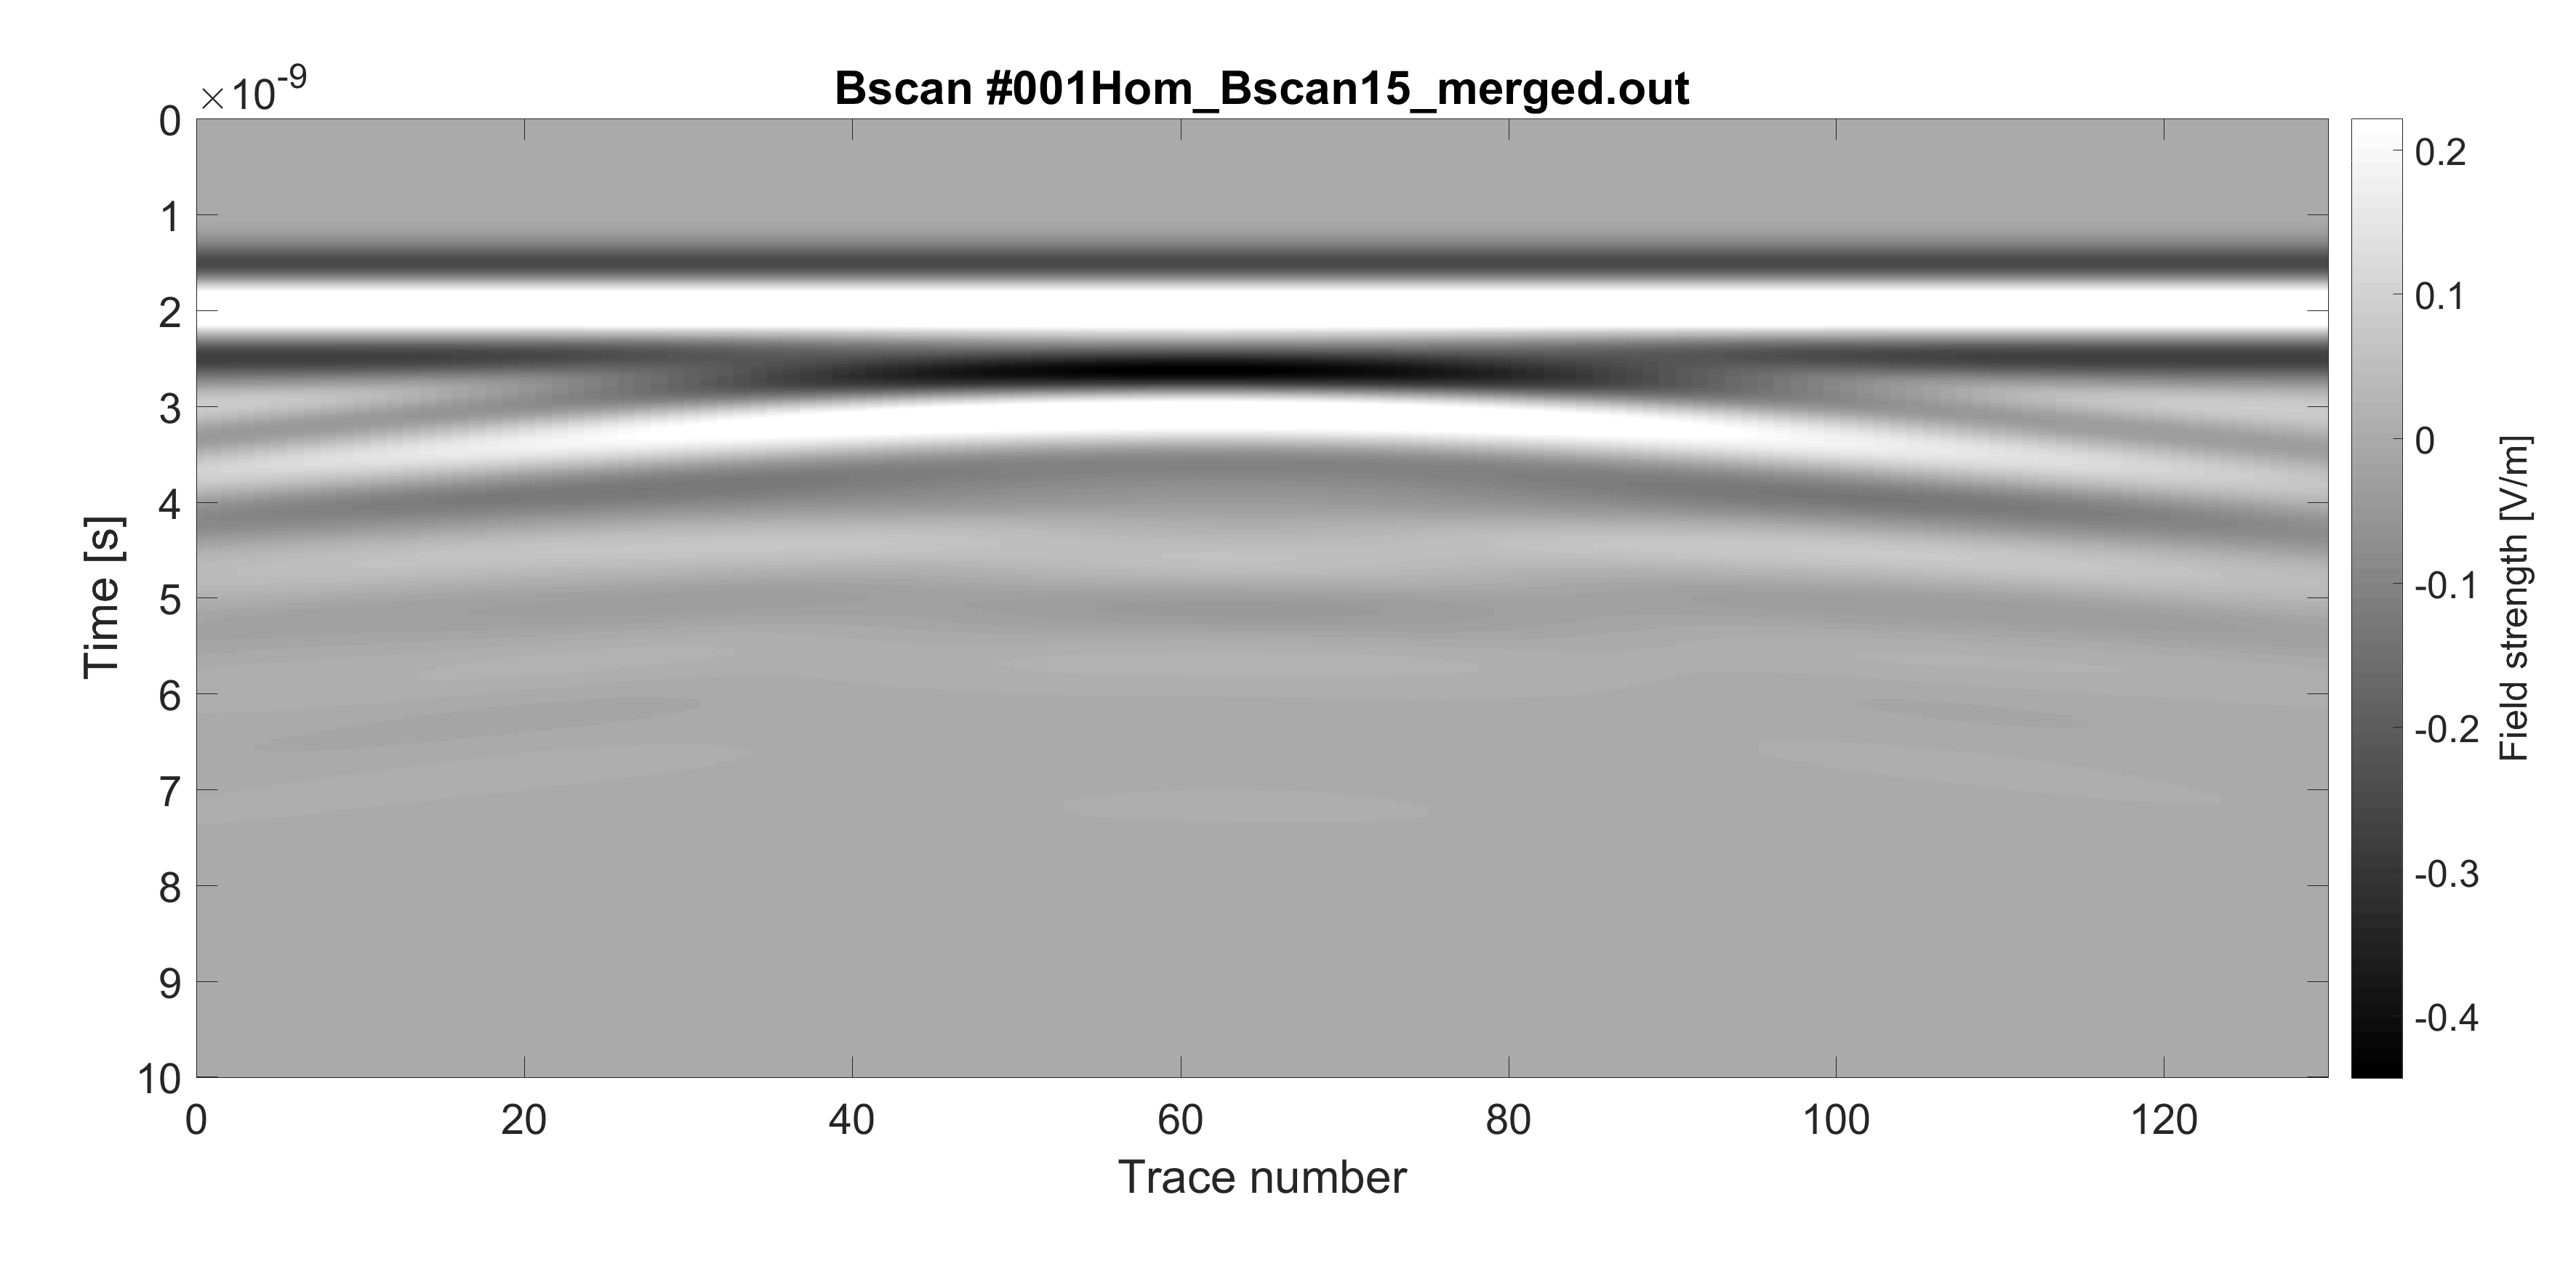
\includegraphics[width=0.47\textwidth, keepaspectratio,valign=c]{Homogeneo/001Hom_Bscan15_merged.png}}
\subfloat{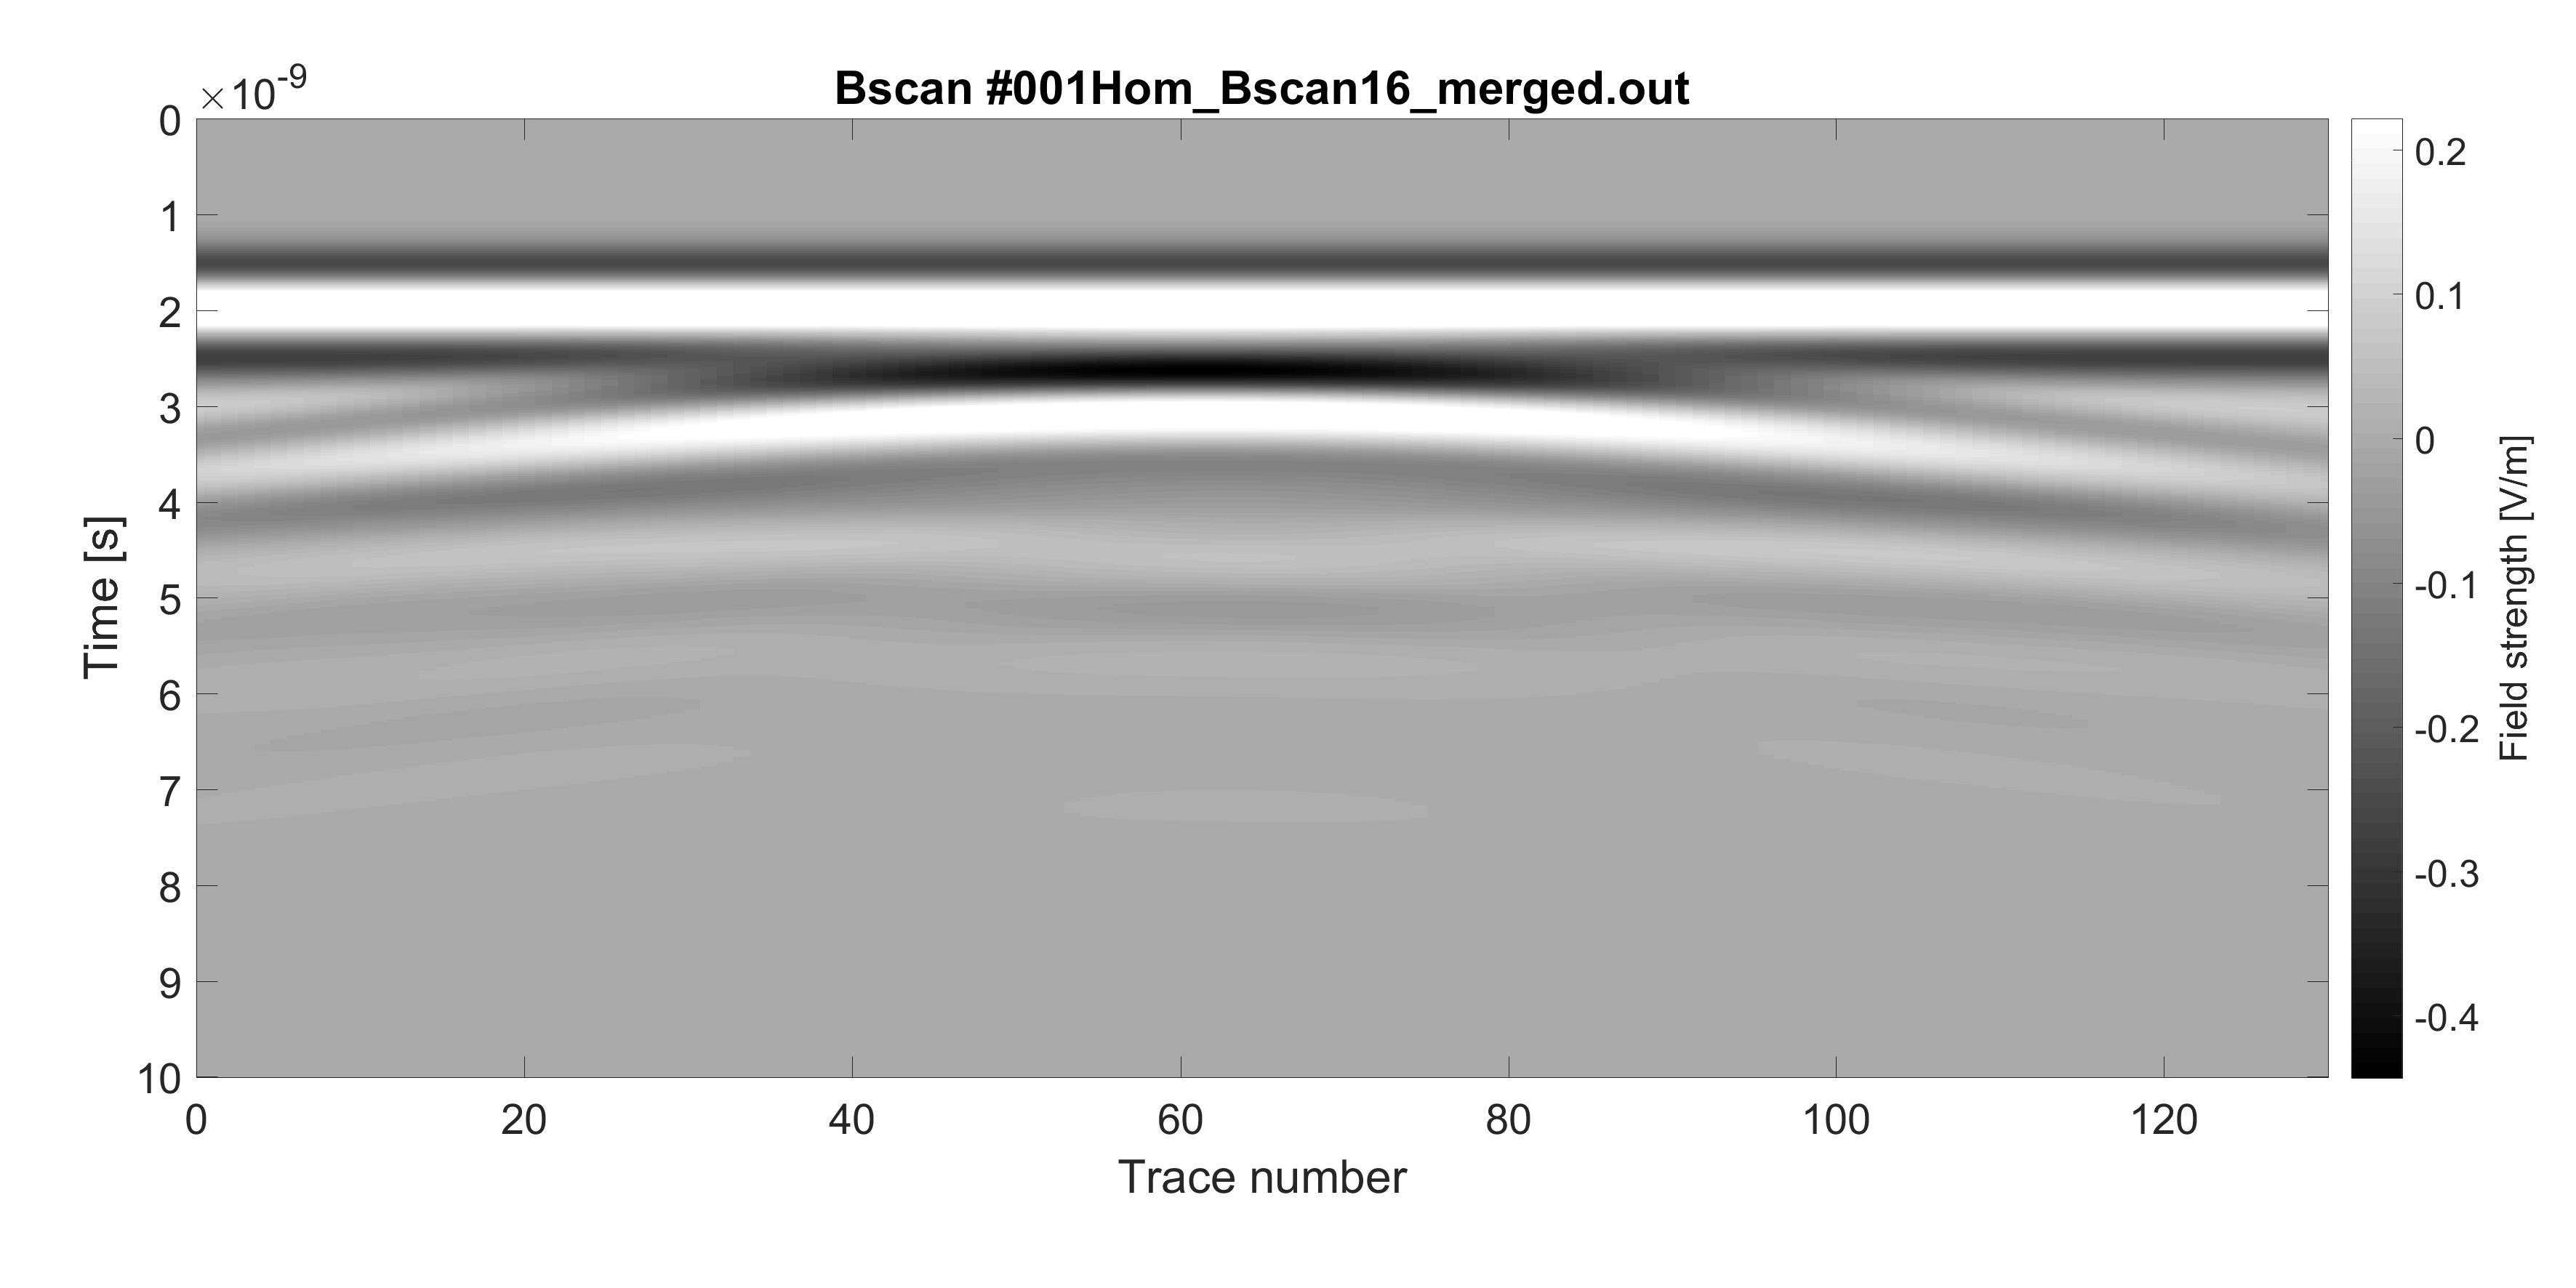
\includegraphics[width=0.47\textwidth, keepaspectratio,valign=c]{Homogeneo/001Hom_Bscan16_merged.png}} 
\subfloat{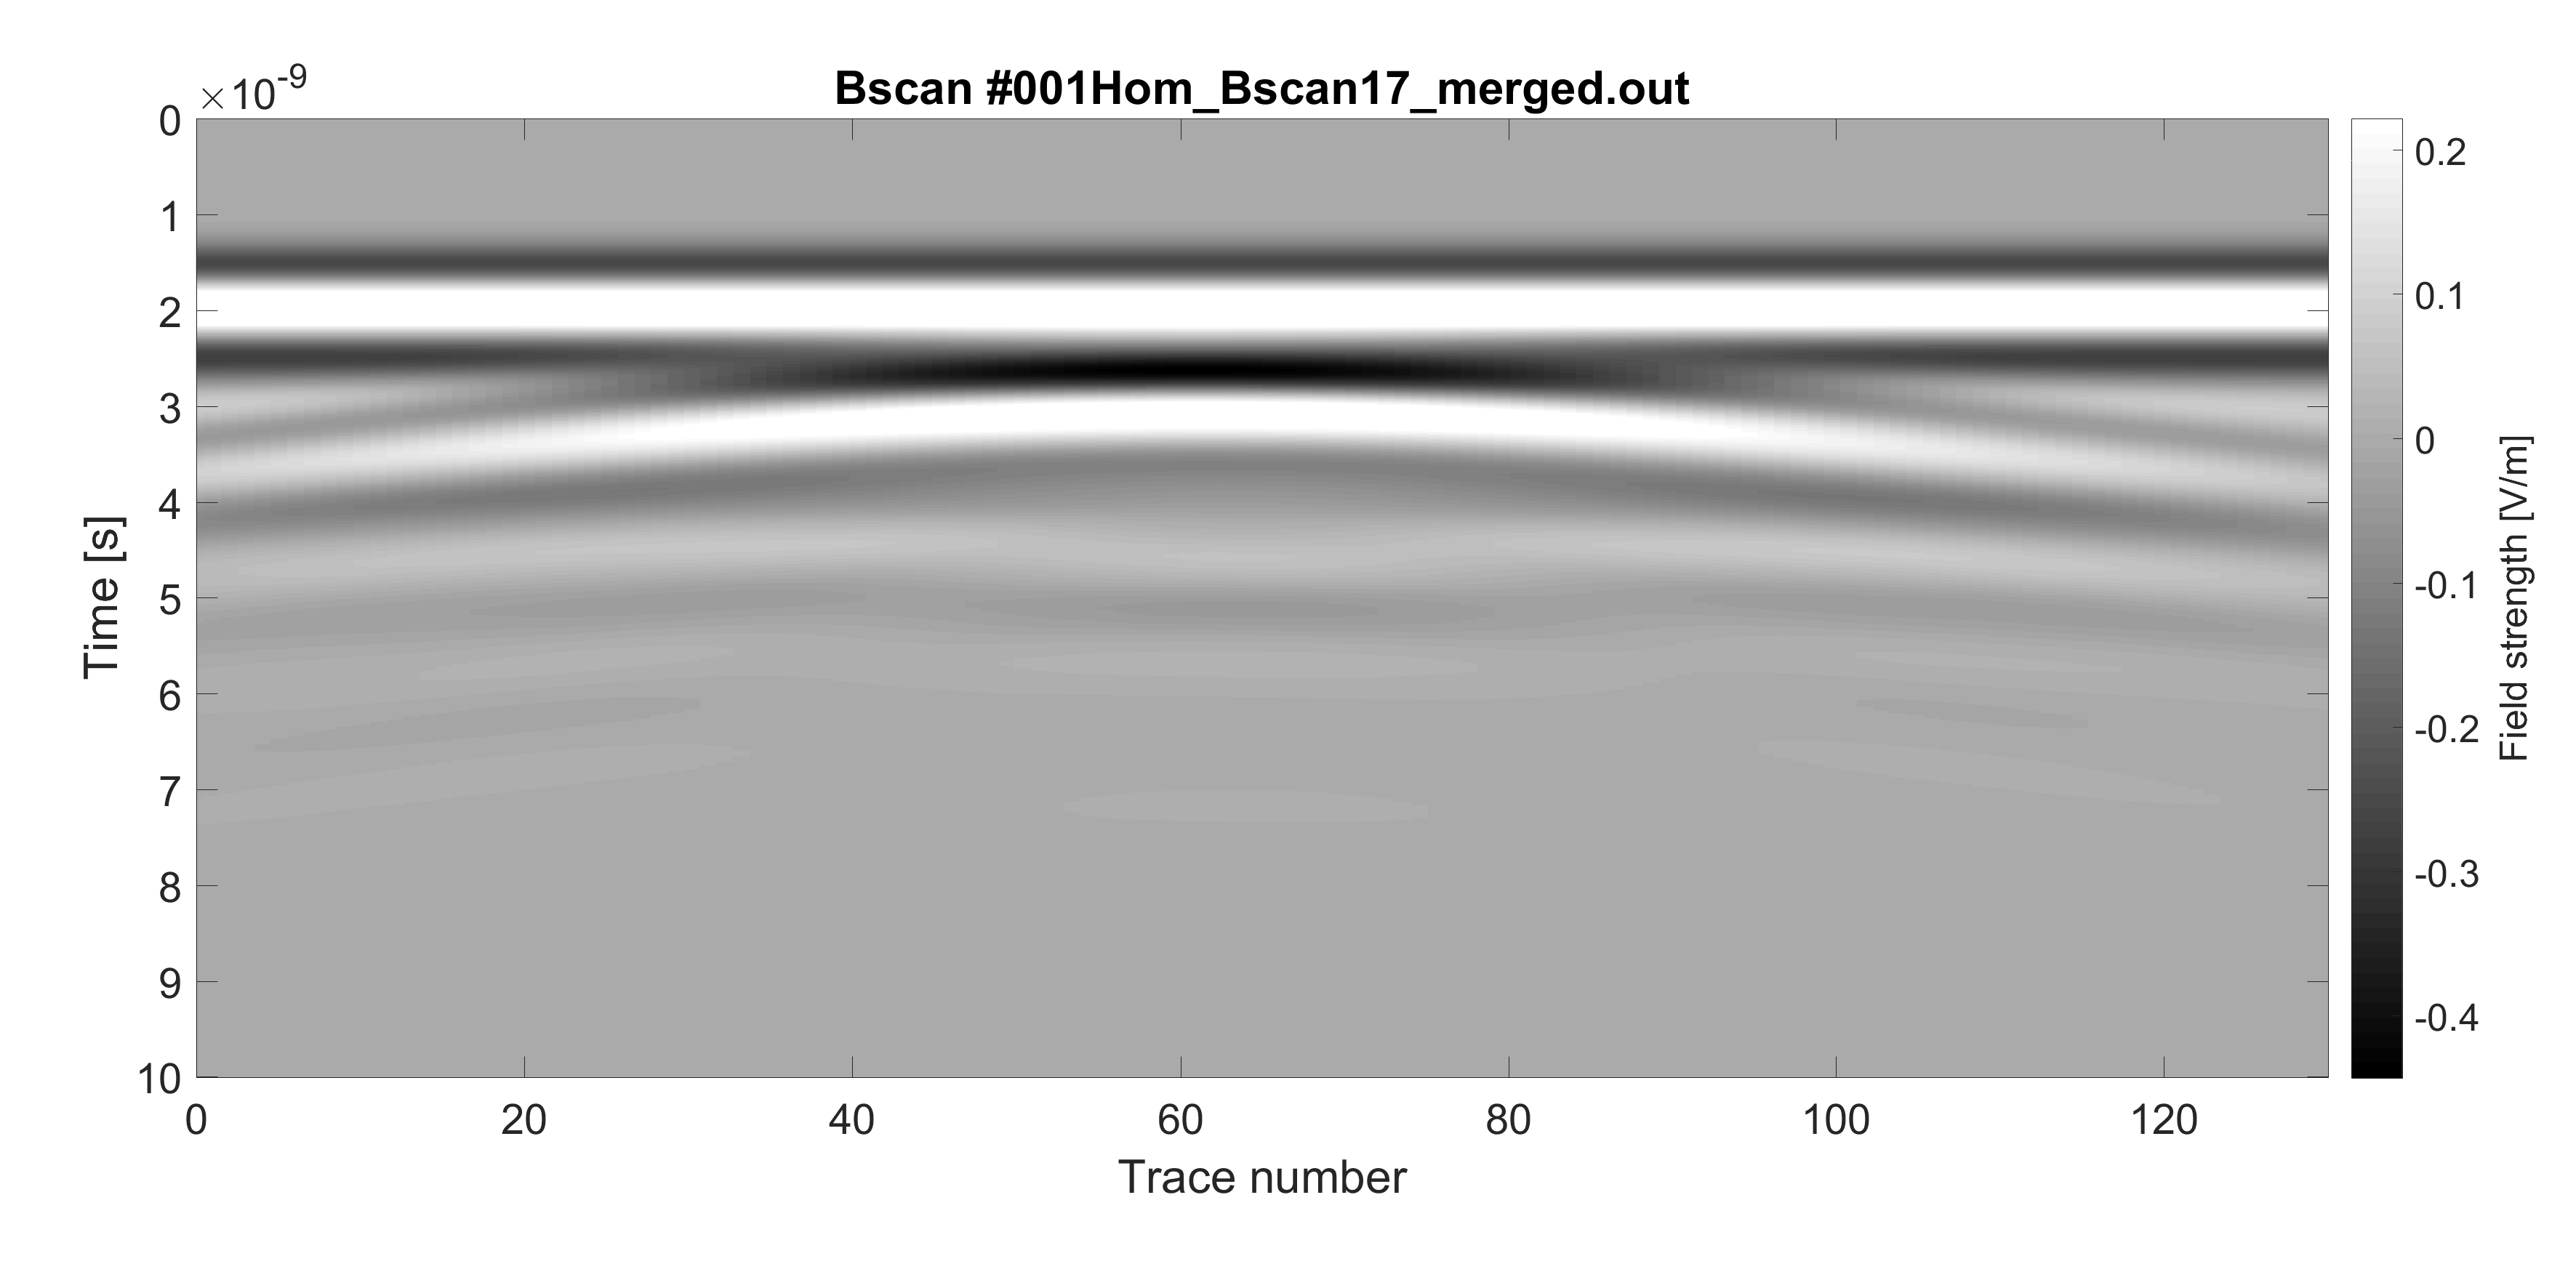
\includegraphics[width=0.47\textwidth, keepaspectratio,valign=c]{Homogeneo/001Hom_Bscan17_merged.png}}
\subfloat{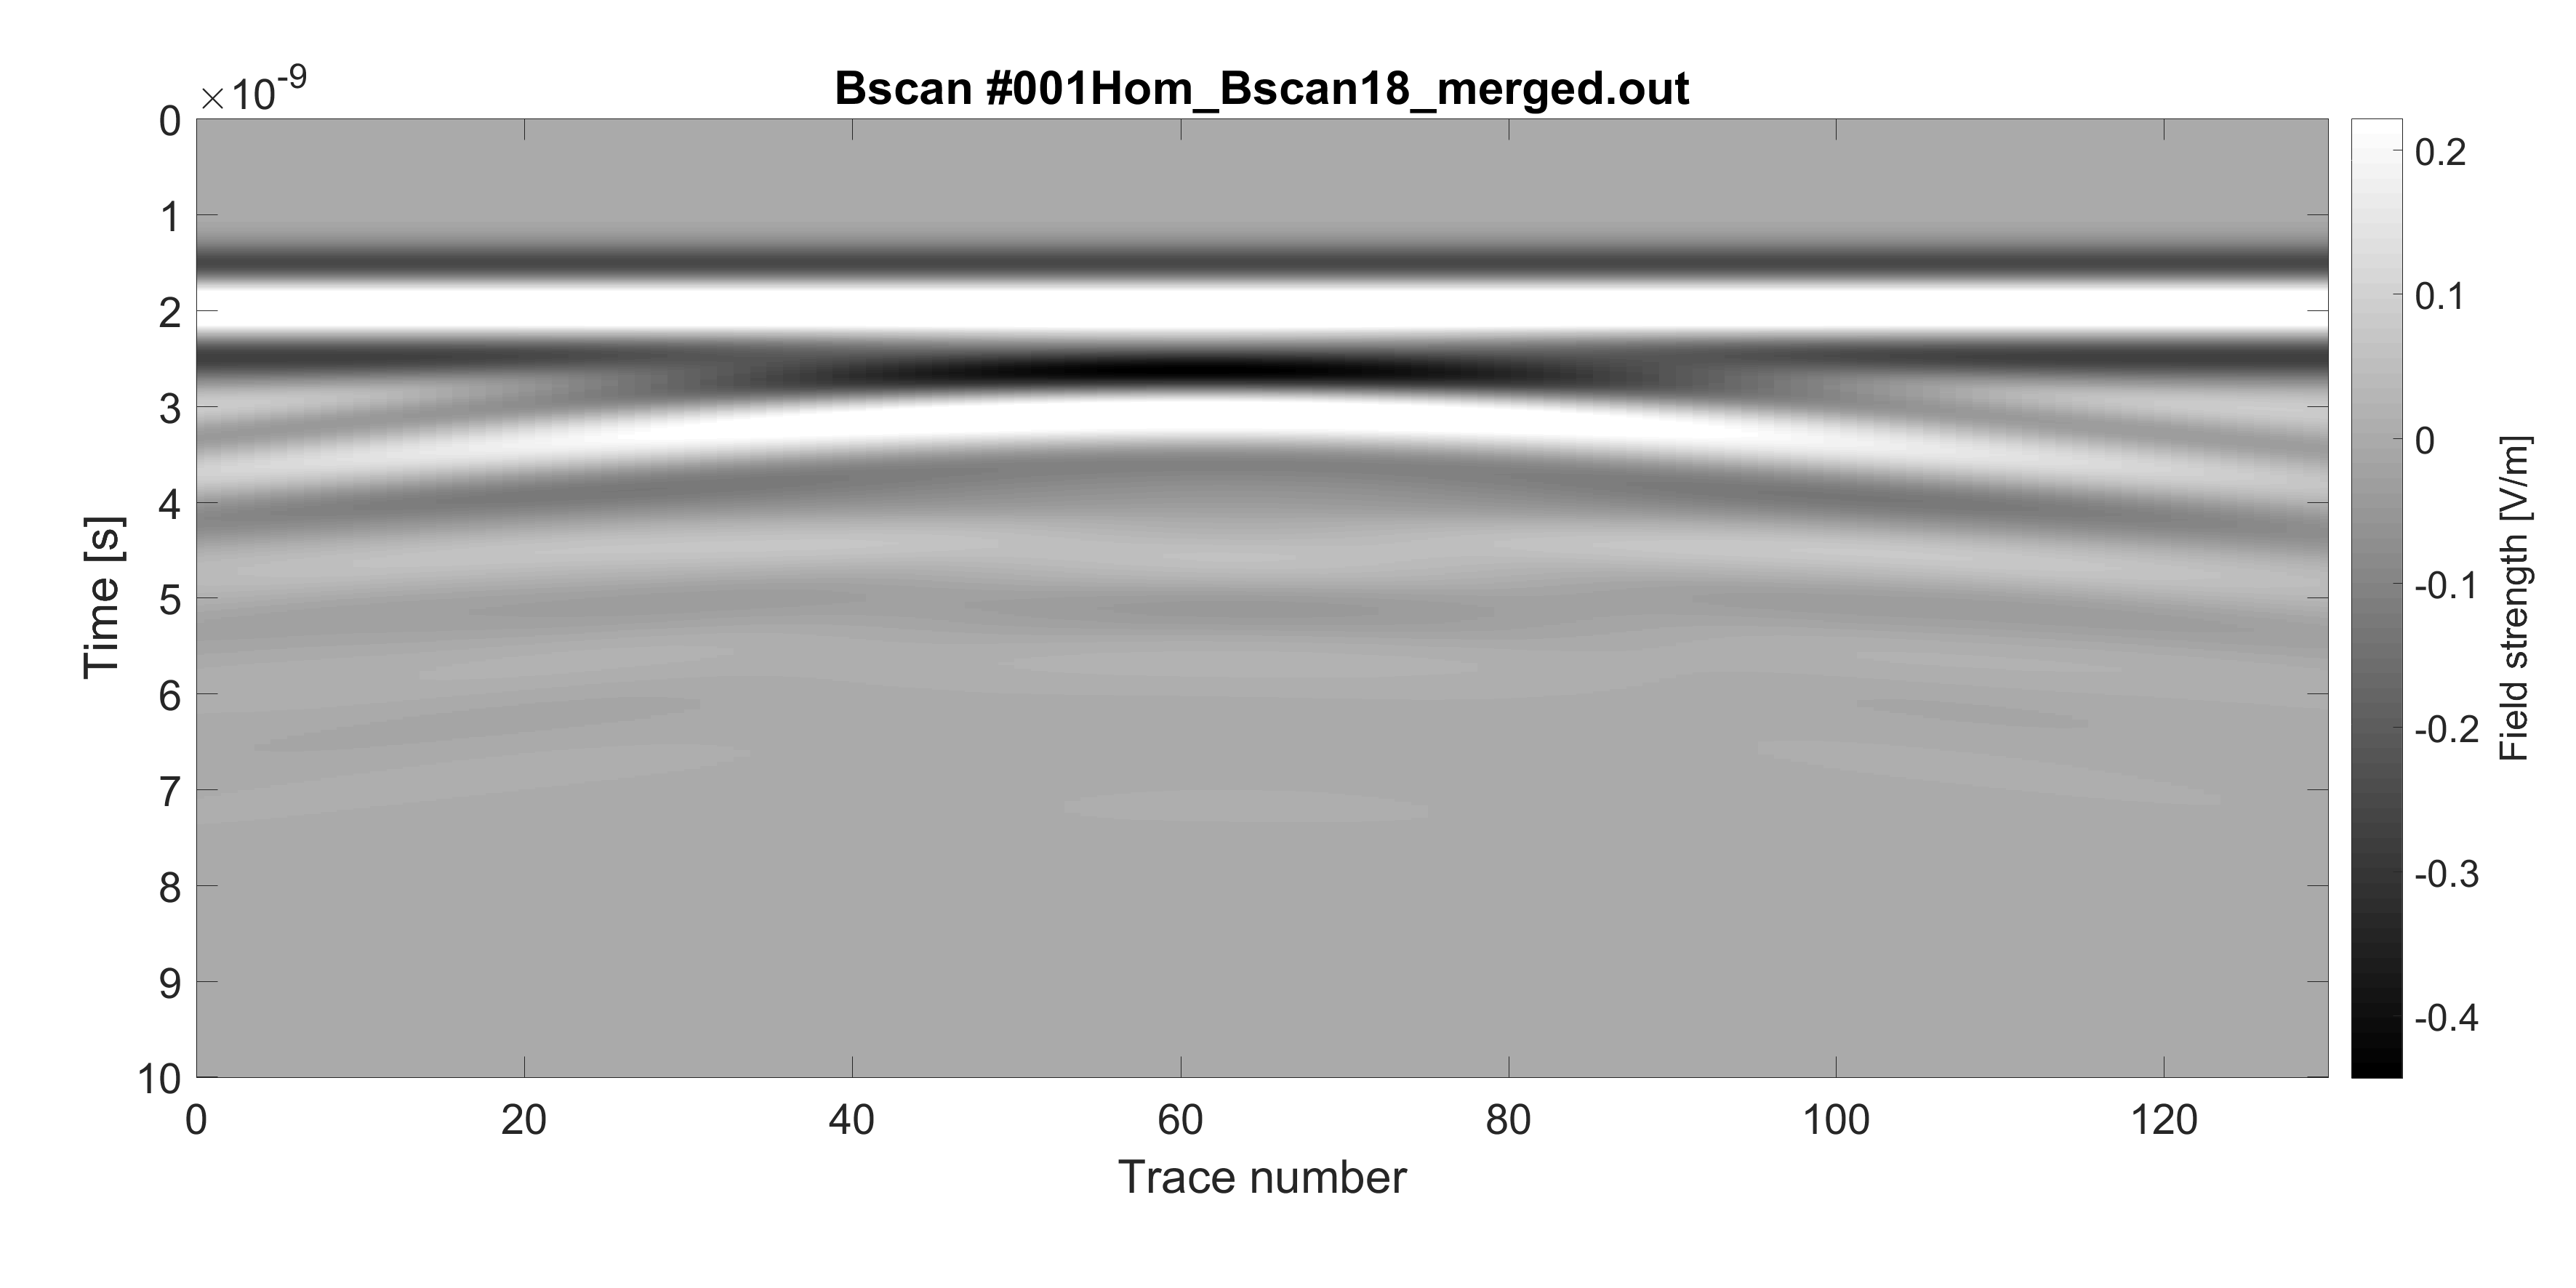
\includegraphics[width=0.47\textwidth, keepaspectratio,valign=c]{Homogeneo/001Hom_Bscan18_merged.png}}
\subfloat{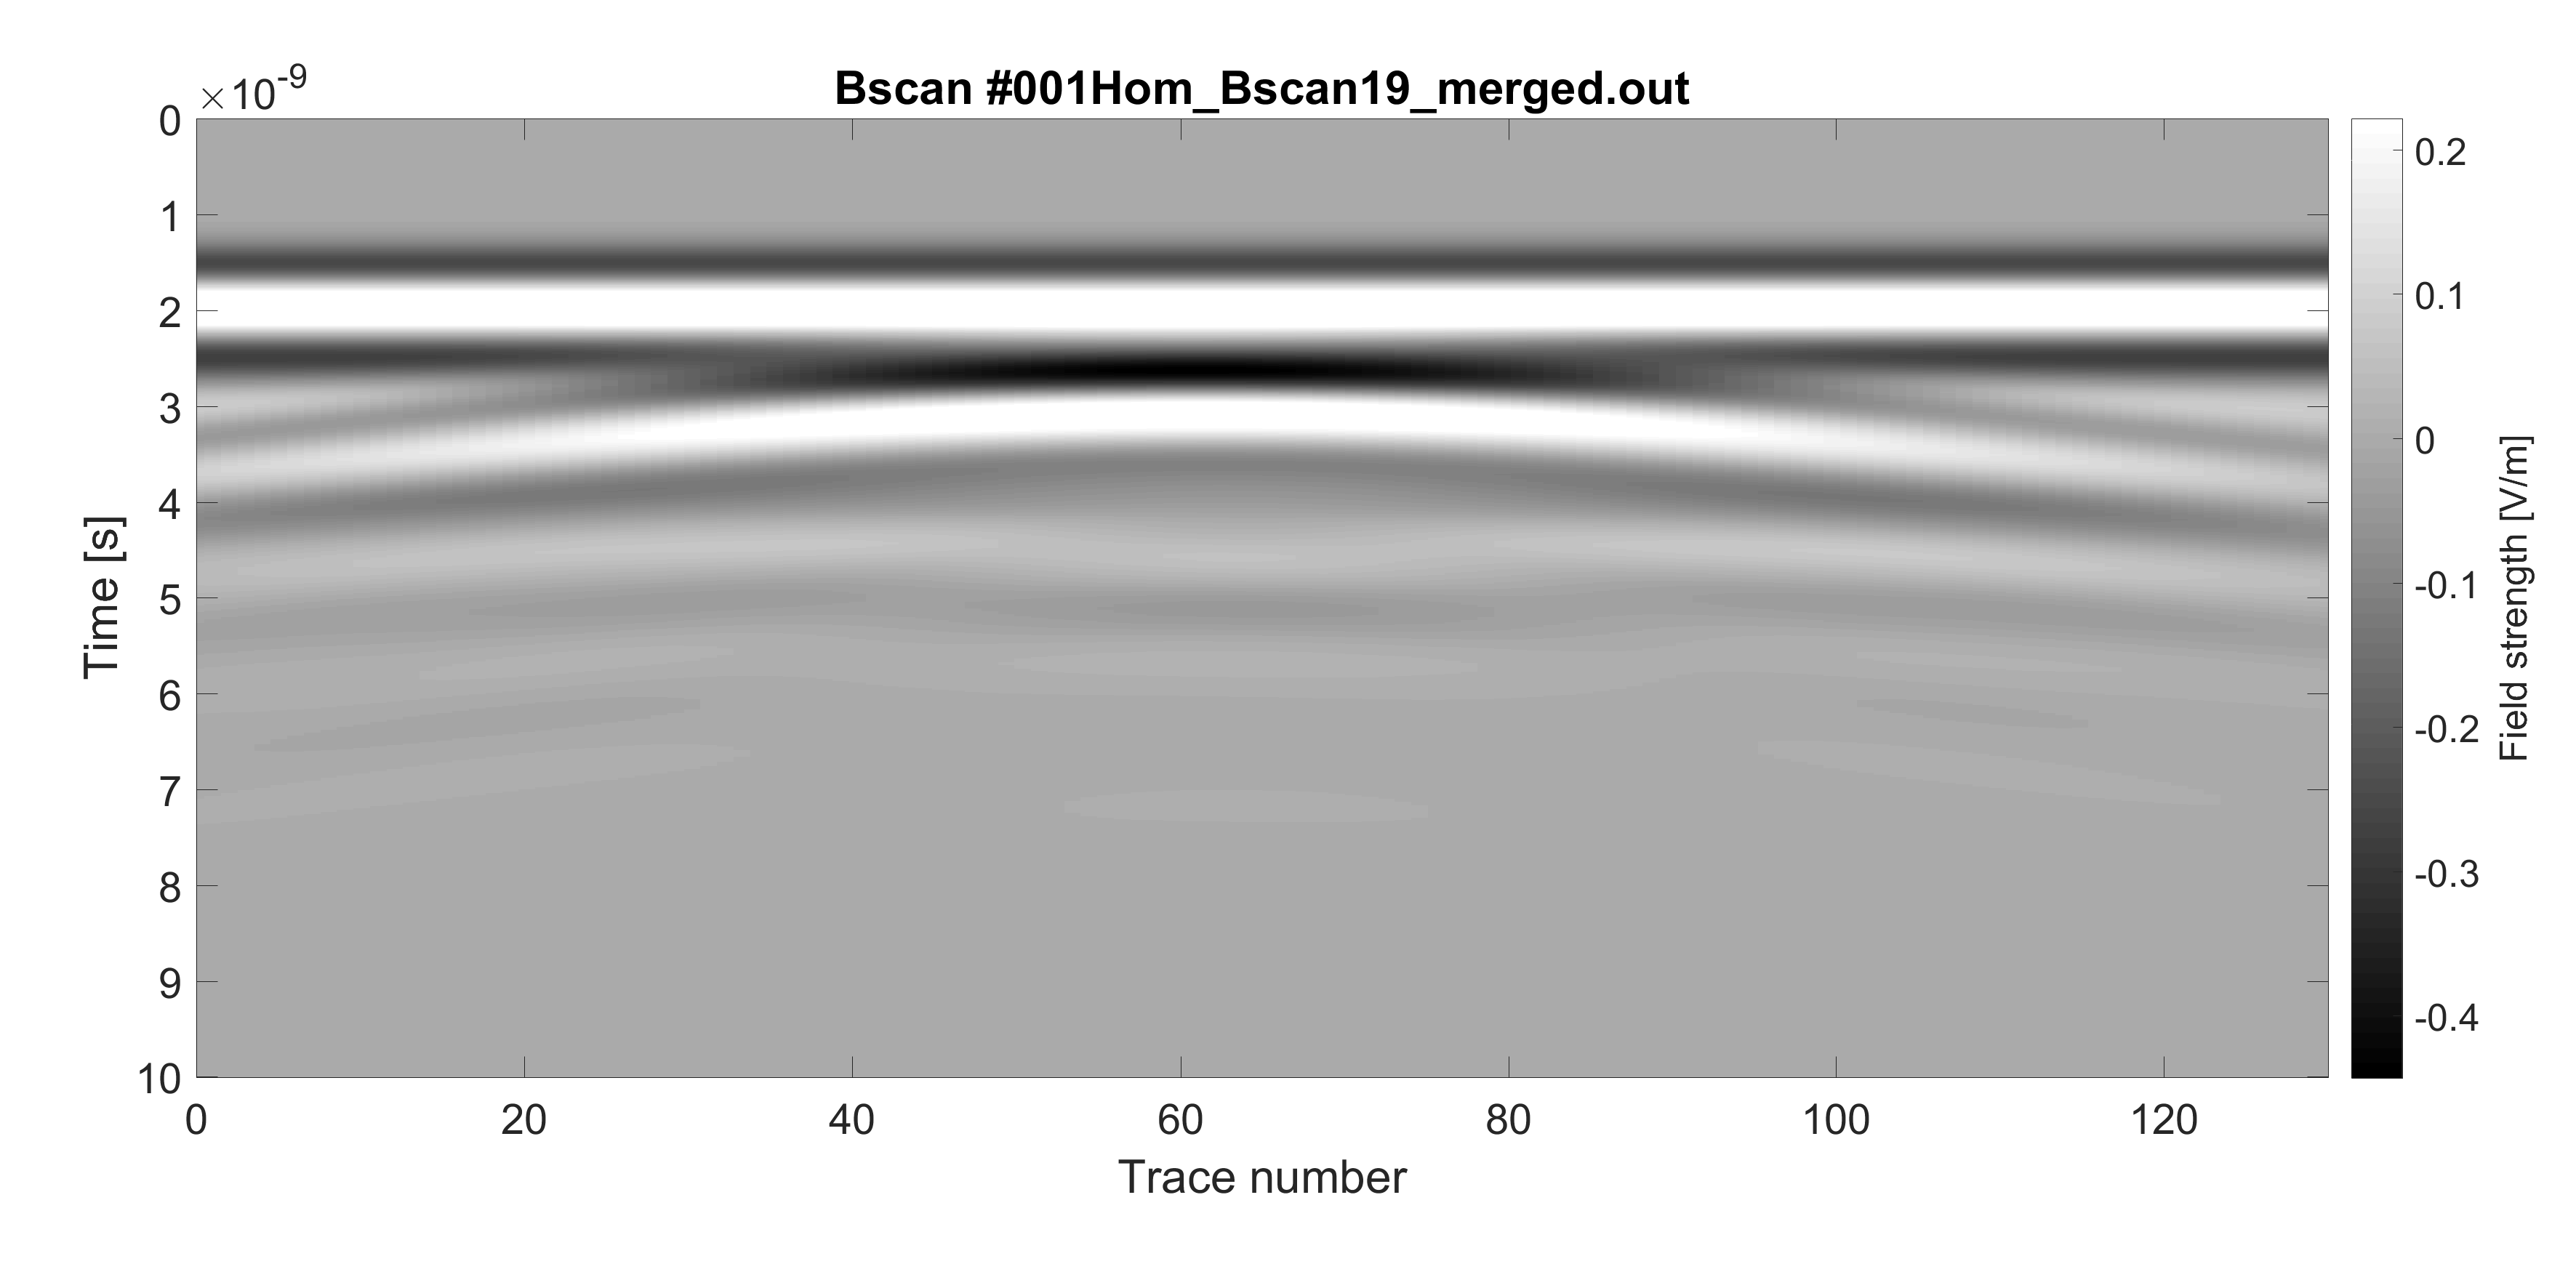
\includegraphics[width=0.47\textwidth, keepaspectratio,valign=c]{Homogeneo/001Hom_Bscan19_merged.png}}
\subfloat{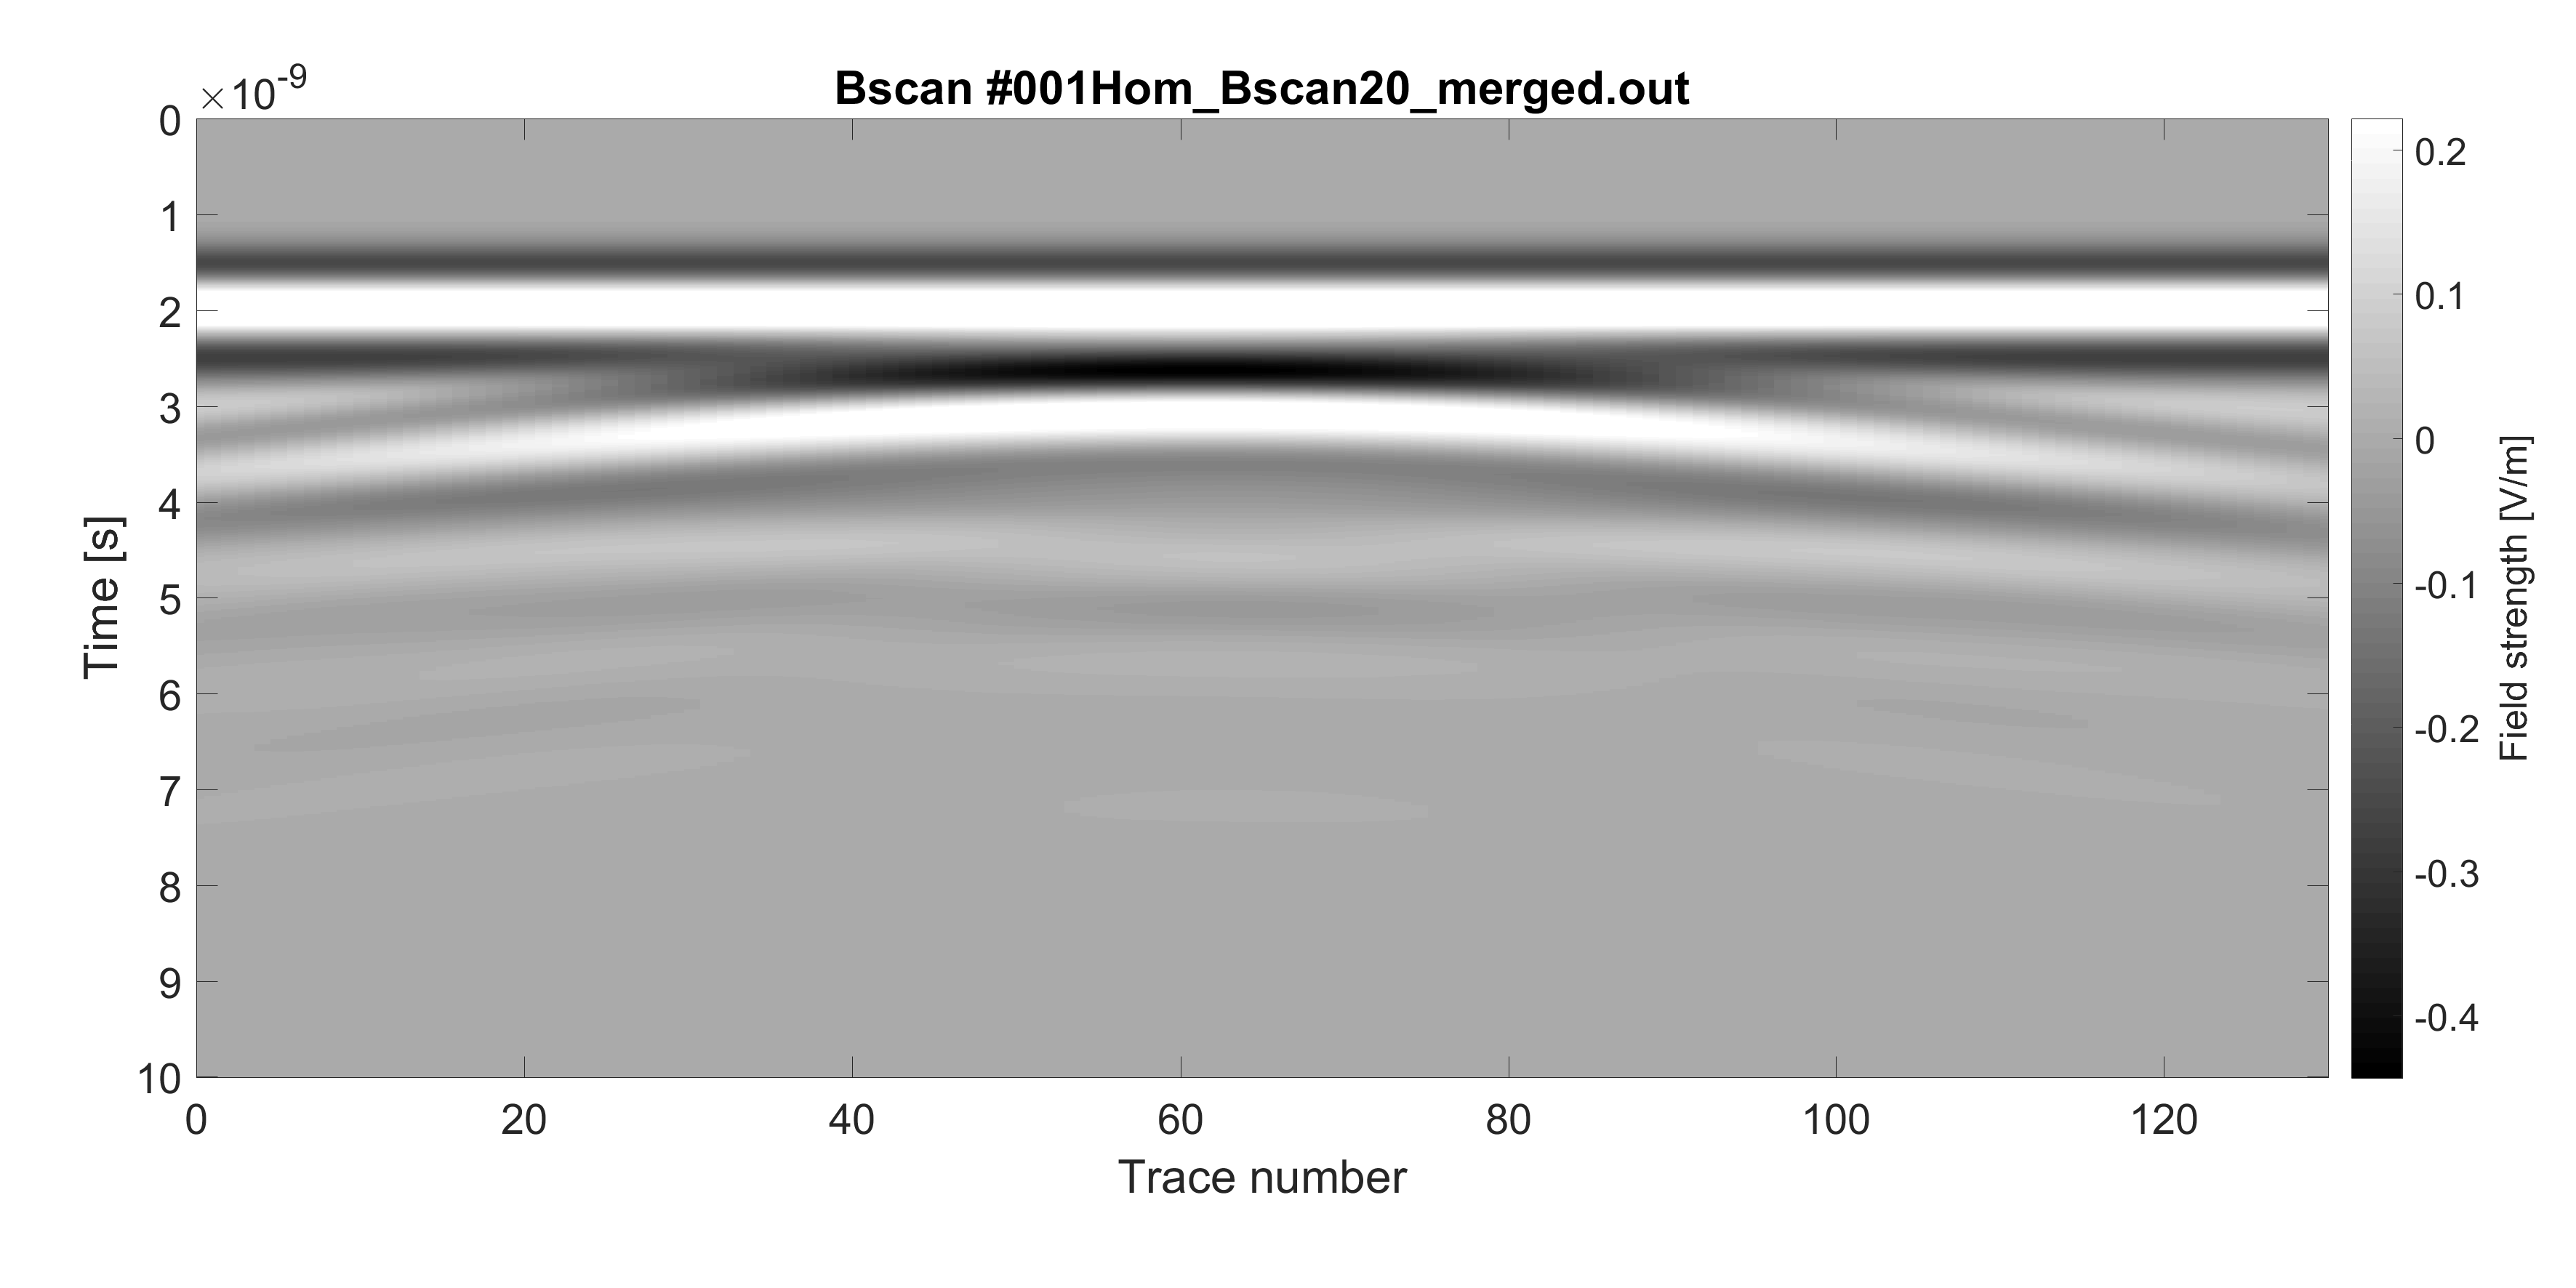
\includegraphics[width=0.47\textwidth, keepaspectratio,valign=c]{Homogeneo/001Hom_Bscan20_merged.png}}
\subfloat{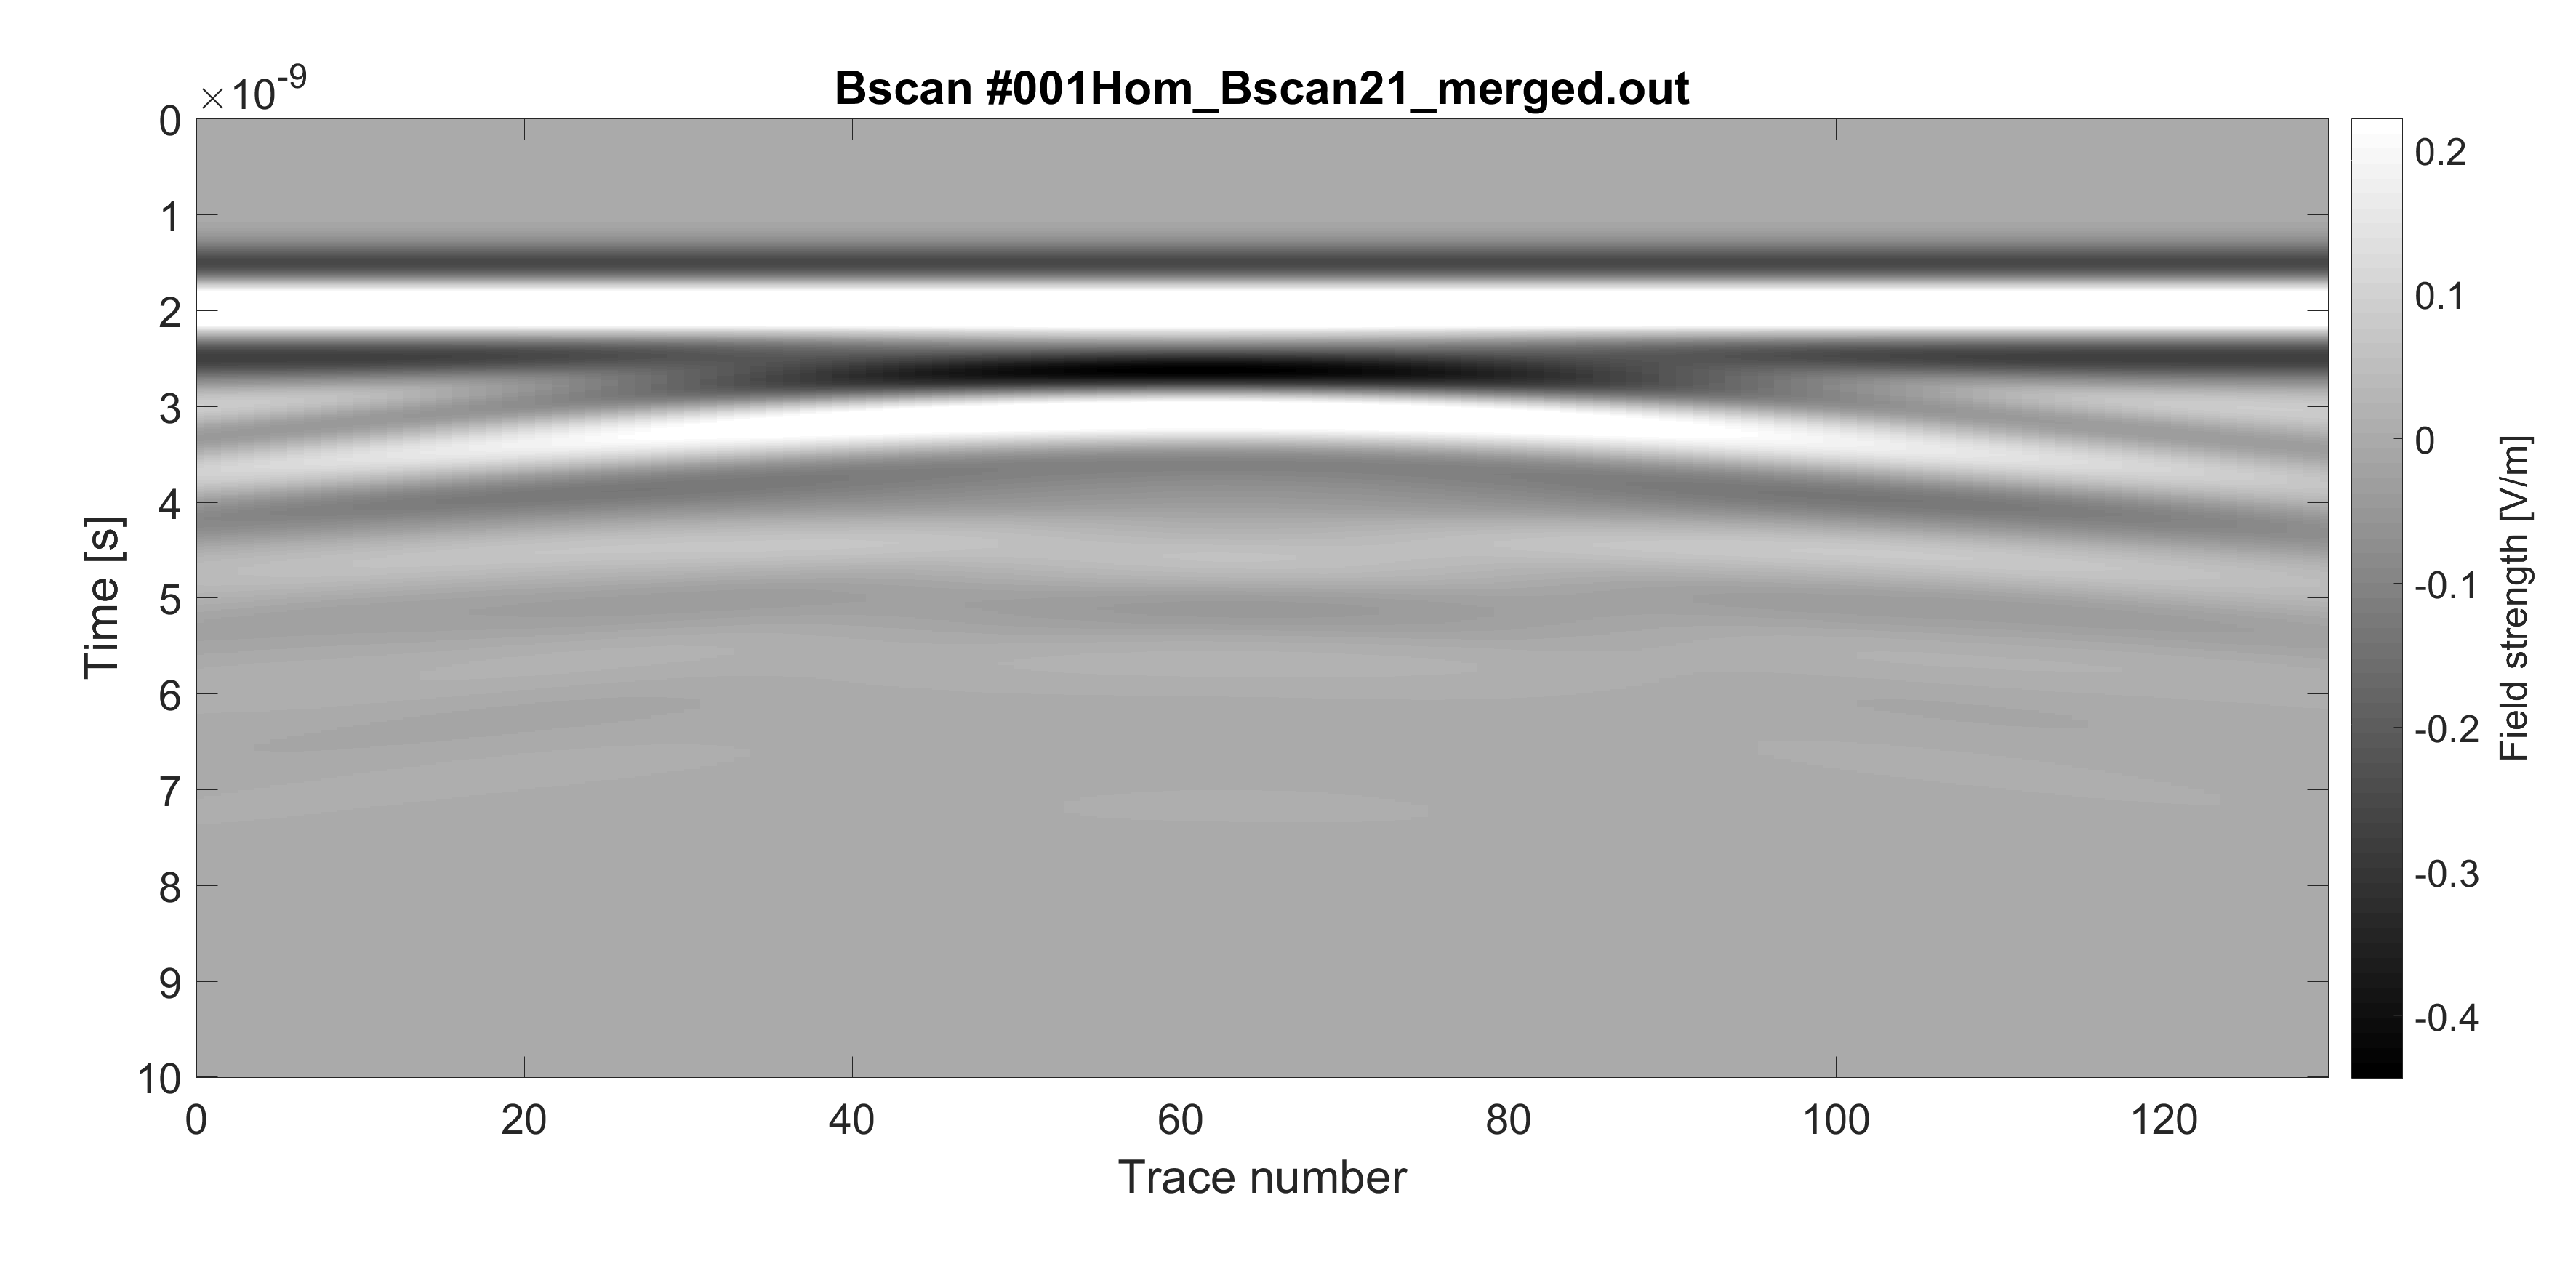
\includegraphics[width=0.47\textwidth, keepaspectratio,valign=c]{Homogeneo/001Hom_Bscan21_merged.png}}
\subfloat{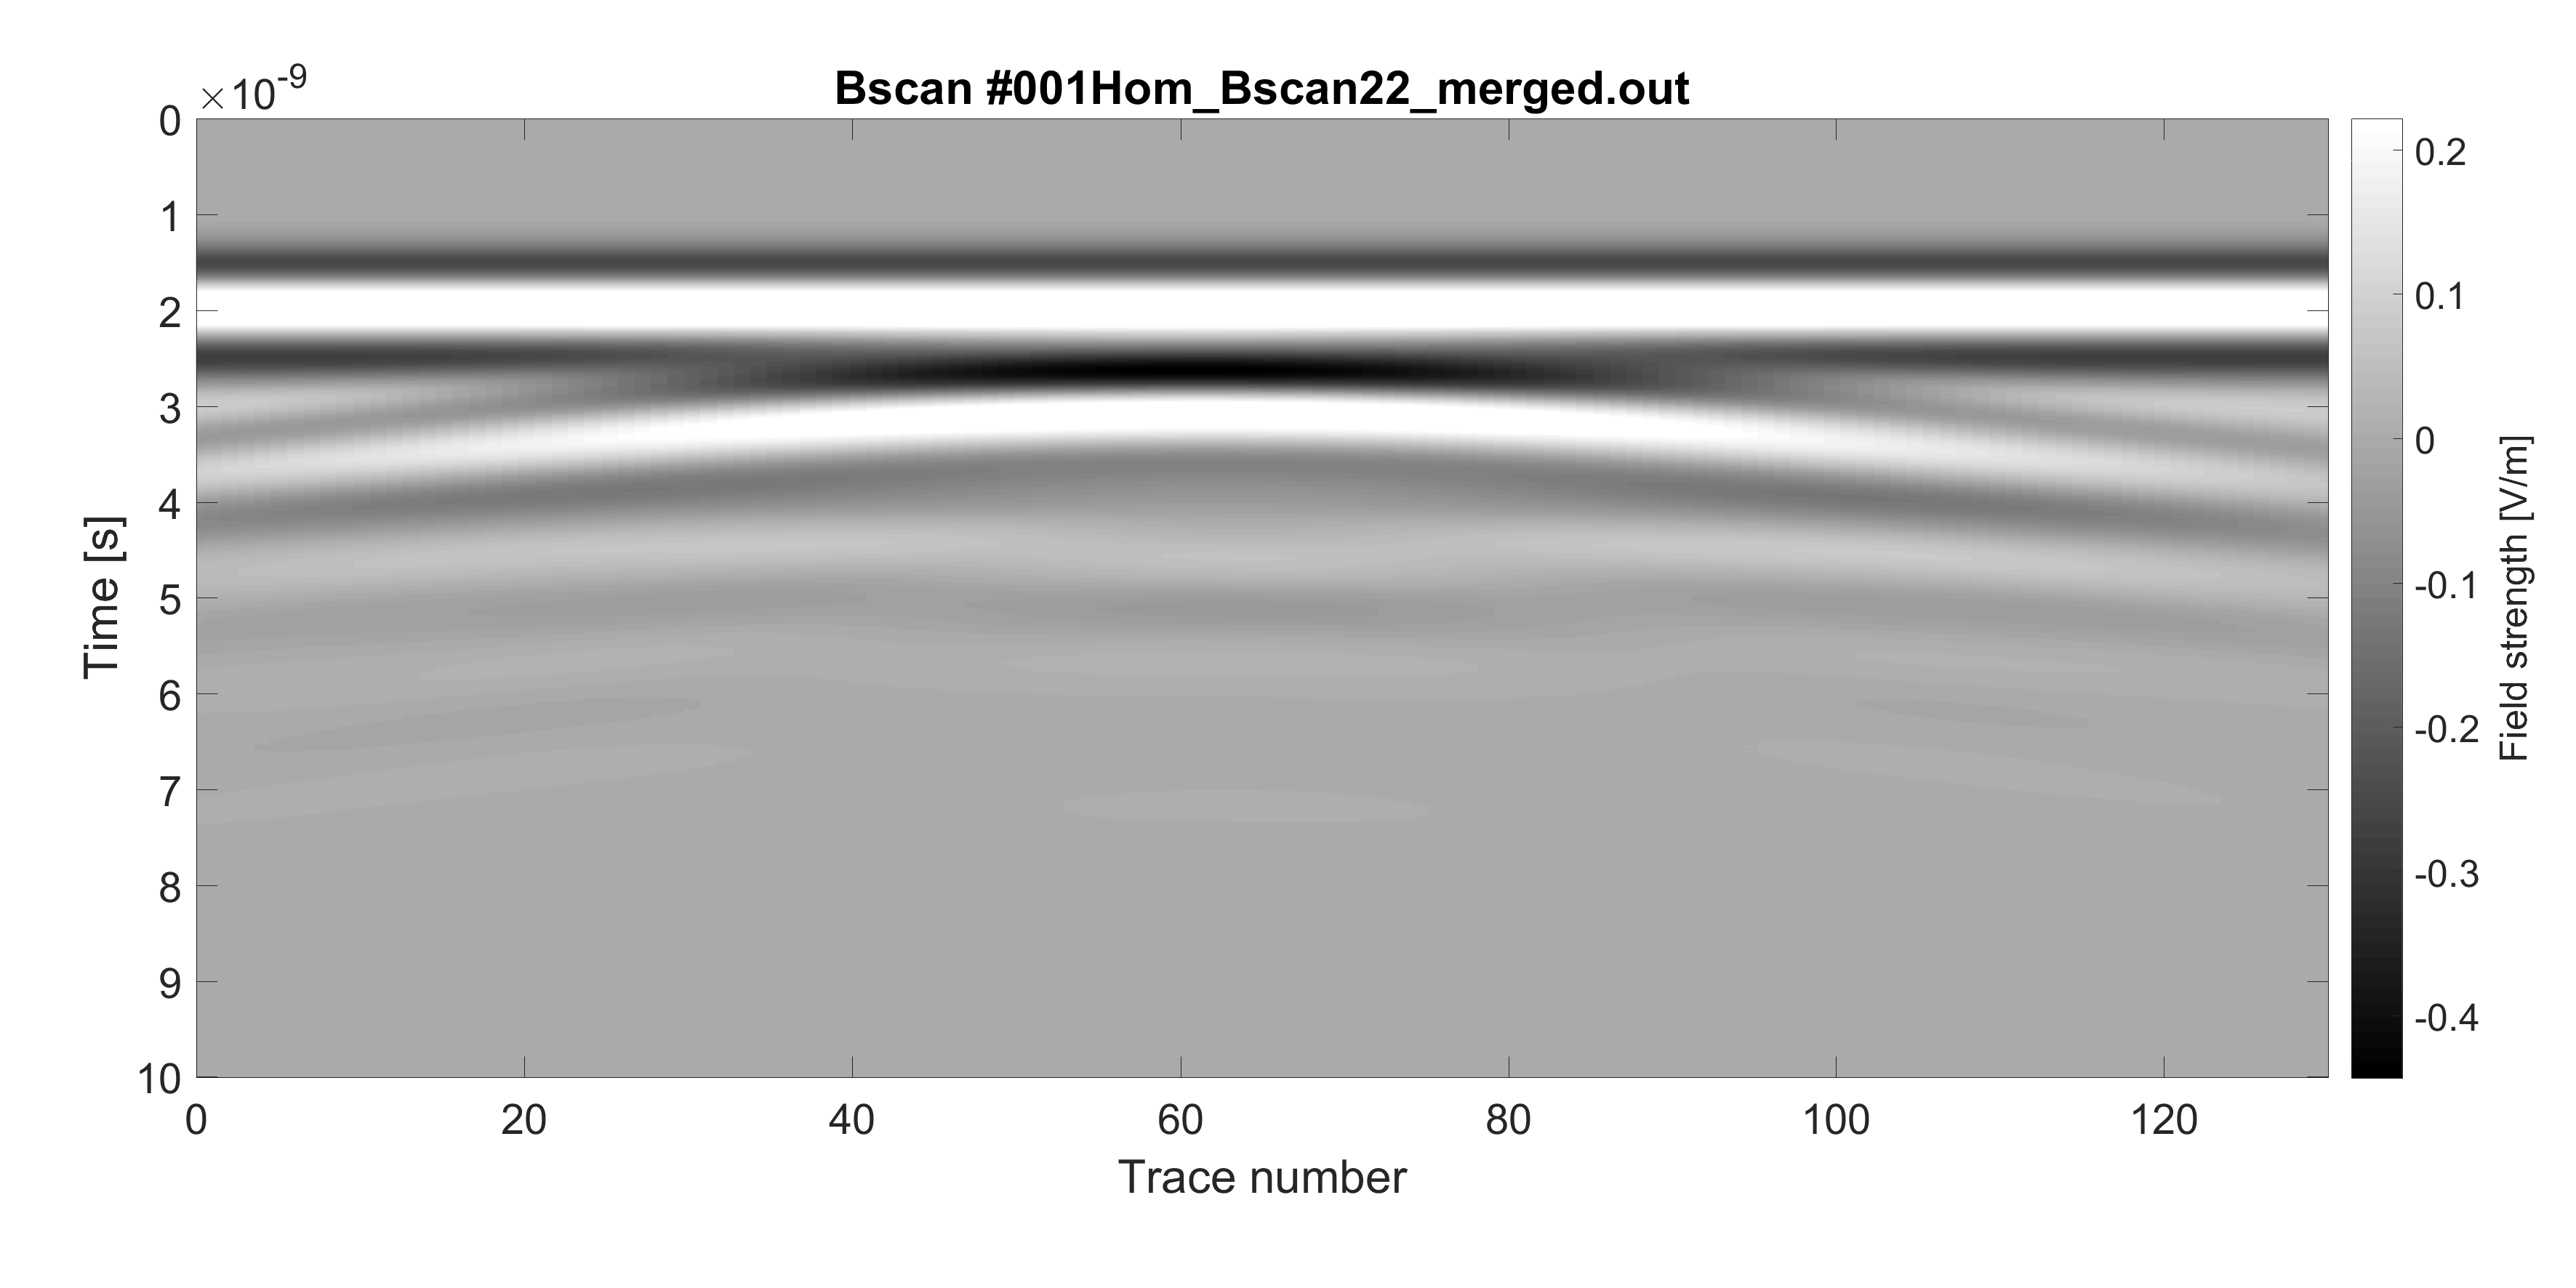
\includegraphics[width=0.47\textwidth, keepaspectratio,valign=c]{Homogeneo/001Hom_Bscan22_merged.png}}
\subfloat{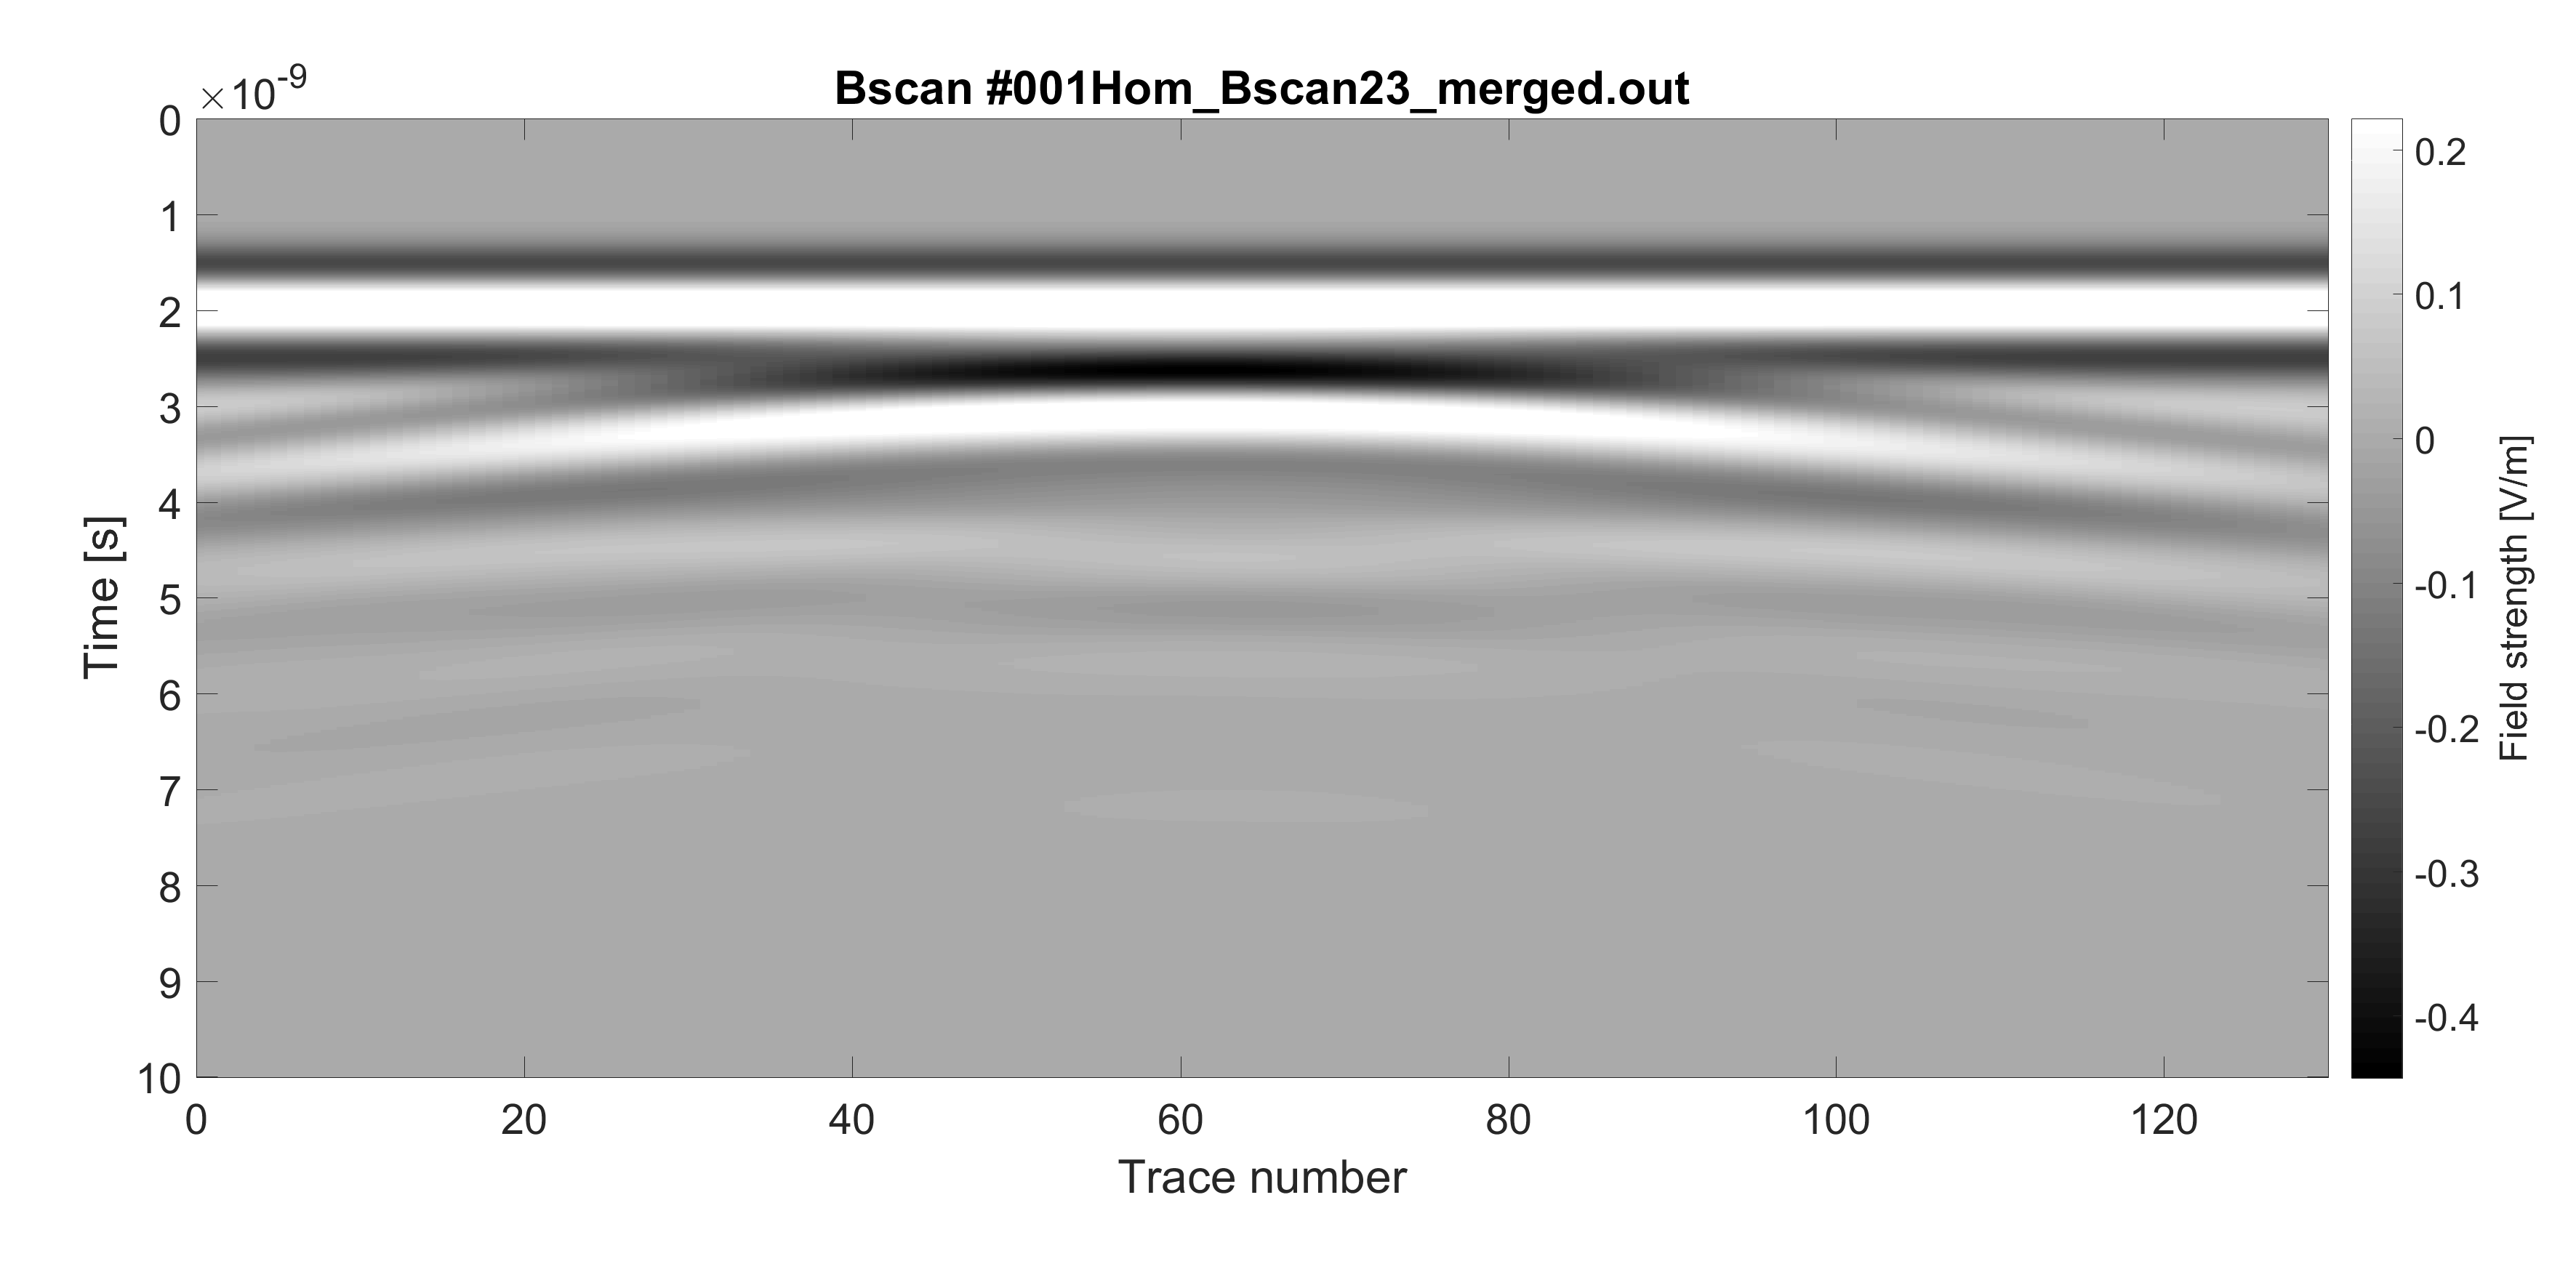
\includegraphics[width=0.47\textwidth, keepaspectratio,valign=c]{Homogeneo/001Hom_Bscan23_merged.png}}
\subfloat{\includegraphics[width=0.47\textwidth, keepaspectratio,valign=c]{Homogeneo/001Hom_Bscan24_merged.png}}
\captionof{figure}{Resultados simulación 001 Original}
\label{fig:001_ORIGINAL}
\end{center}



\subsubsubsection{RPCA}
\begin{center}
\CT
\subfloat{\includegraphics[width=0.47\textwidth, keepaspectratio,valign=c]{Homogeneo/001Hom_Bscan1_merged_Sparse.png}}
\subfloat{\includegraphics[width=0.47\textwidth, keepaspectratio,valign=c]{Homogeneo/001Hom_Bscan2_merged_Sparse.png}}
\subfloat{\includegraphics[width=0.47\textwidth, keepaspectratio,valign=c]{Homogeneo/001Hom_Bscan3_merged_Sparse.png}}
\subfloat{\includegraphics[width=0.47\textwidth, keepaspectratio,valign=c]{Homogeneo/001Hom_Bscan4_merged_Sparse.png}}
\subfloat{\includegraphics[width=0.47\textwidth, keepaspectratio,valign=c]{Homogeneo/001Hom_Bscan5_merged_Sparse.png}}
\subfloat{\includegraphics[width=0.47\textwidth, keepaspectratio,valign=c]{Homogeneo/001Hom_Bscan6_merged_Sparse.png}} 
\subfloat{\includegraphics[width=0.47\textwidth, keepaspectratio,valign=c]{Homogeneo/001Hom_Bscan7_merged_Sparse.png}}
\subfloat{\includegraphics[width=0.47\textwidth, keepaspectratio,valign=c]{Homogeneo/001Hom_Bscan8_merged_Sparse.png}}
\subfloat{\includegraphics[width=0.47\textwidth, keepaspectratio,valign=c]{Homogeneo/001Hom_Bscan9_merged_Sparse.png}}
\subfloat{\includegraphics[width=0.47\textwidth, keepaspectratio,valign=c]{Homogeneo/001Hom_Bscan10_merged_Sparse.png}} 
\subfloat{\includegraphics[width=0.47\textwidth, keepaspectratio,valign=c]{Homogeneo/001Hom_Bscan11_merged_Sparse.png}}
\subfloat{\includegraphics[width=0.47\textwidth, keepaspectratio,valign=c]{Homogeneo/001Hom_Bscan12_merged_Sparse.png}}
\subfloat{\includegraphics[width=0.47\textwidth, keepaspectratio,valign=c]{Homogeneo/001Hom_Bscan13_merged_Sparse.png}}
\subfloat{\includegraphics[width=0.47\textwidth, keepaspectratio,valign=c]{Homogeneo/001Hom_Bscan14_merged_Sparse.png}}
\subfloat{\includegraphics[width=0.47\textwidth, keepaspectratio,valign=c]{Homogeneo/001Hom_Bscan15_merged_Sparse.png}}
\subfloat{\includegraphics[width=0.47\textwidth, keepaspectratio,valign=c]{Homogeneo/001Hom_Bscan16_merged_Sparse.png}} 
\subfloat{\includegraphics[width=0.47\textwidth, keepaspectratio,valign=c]{Homogeneo/001Hom_Bscan17_merged_Sparse.png}}
\subfloat{\includegraphics[width=0.47\textwidth, keepaspectratio,valign=c]{Homogeneo/001Hom_Bscan18_merged_Sparse.png}}
\subfloat{\includegraphics[width=0.47\textwidth, keepaspectratio,valign=c]{Homogeneo/001Hom_Bscan19_merged_Sparse.png}}
\subfloat{\includegraphics[width=0.47\textwidth, keepaspectratio,valign=c]{Homogeneo/001Hom_Bscan20_merged_Sparse.png}}
\subfloat{\includegraphics[width=0.47\textwidth, keepaspectratio,valign=c]{Homogeneo/001Hom_Bscan21_merged_Sparse.png}}
\subfloat{\includegraphics[width=0.47\textwidth, keepaspectratio,valign=c]{Homogeneo/001Hom_Bscan22_merged_Sparse.png}}
\subfloat{\includegraphics[width=0.47\textwidth, keepaspectratio,valign=c]{Homogeneo/001Hom_Bscan23_merged_Sparse.png}}
\subfloat{\includegraphics[width=0.47\textwidth, keepaspectratio,valign=c]{Homogeneo/001Hom_Bscan24_merged_Sparse.png}}
\captionof{figure}{Resultados simulación 001 Sparse de RPCA}
\label{fig:001_RPCA_SPARSE}
\end{center}


\begin{center}
\CT
\subfloat{\includegraphics[width=0.47\textwidth, keepaspectratio,valign=c]{Homogeneo/001Hom_Bscan1_merged_LowRank.png}}
\subfloat{\includegraphics[width=0.47\textwidth, keepaspectratio,valign=c]{Homogeneo/001Hom_Bscan2_merged_LowRank.png}}
\subfloat{\includegraphics[width=0.47\textwidth, keepaspectratio,valign=c]{Homogeneo/001Hom_Bscan3_merged_LowRank.png}}
\subfloat{\includegraphics[width=0.47\textwidth, keepaspectratio,valign=c]{Homogeneo/001Hom_Bscan4_merged_LowRank.png}}
\subfloat{\includegraphics[width=0.47\textwidth, keepaspectratio,valign=c]{Homogeneo/001Hom_Bscan5_merged_LowRank.png}}
\subfloat{\includegraphics[width=0.47\textwidth, keepaspectratio,valign=c]{Homogeneo/001Hom_Bscan6_merged_LowRank.png}} 
\subfloat{\includegraphics[width=0.47\textwidth, keepaspectratio,valign=c]{Homogeneo/001Hom_Bscan7_merged_LowRank.png}}
\subfloat{\includegraphics[width=0.47\textwidth, keepaspectratio,valign=c]{Homogeneo/001Hom_Bscan8_merged_LowRank.png}}
\subfloat{\includegraphics[width=0.47\textwidth, keepaspectratio,valign=c]{Homogeneo/001Hom_Bscan9_merged_LowRank.png}}
\subfloat{\includegraphics[width=0.47\textwidth, keepaspectratio,valign=c]{Homogeneo/001Hom_Bscan10_merged_LowRank.png}} 
\subfloat{\includegraphics[width=0.47\textwidth, keepaspectratio,valign=c]{Homogeneo/001Hom_Bscan11_merged_LowRank.png}}
\subfloat{\includegraphics[width=0.47\textwidth, keepaspectratio,valign=c]{Homogeneo/001Hom_Bscan12_merged_LowRank.png}}
\subfloat{\includegraphics[width=0.47\textwidth, keepaspectratio,valign=c]{Homogeneo/001Hom_Bscan13_merged_LowRank.png}}
\subfloat{\includegraphics[width=0.47\textwidth, keepaspectratio,valign=c]{Homogeneo/001Hom_Bscan14_merged_LowRank.png}}
\subfloat{\includegraphics[width=0.47\textwidth, keepaspectratio,valign=c]{Homogeneo/001Hom_Bscan15_merged_LowRank.png}}
\subfloat{\includegraphics[width=0.47\textwidth, keepaspectratio,valign=c]{Homogeneo/001Hom_Bscan16_merged_LowRank.png}} 
\subfloat{\includegraphics[width=0.47\textwidth, keepaspectratio,valign=c]{Homogeneo/001Hom_Bscan17_merged_LowRank.png}}
\subfloat{\includegraphics[width=0.47\textwidth, keepaspectratio,valign=c]{Homogeneo/001Hom_Bscan18_merged_LowRank.png}}
\subfloat{\includegraphics[width=0.47\textwidth, keepaspectratio,valign=c]{Homogeneo/001Hom_Bscan19_merged_LowRank.png}}
\subfloat{\includegraphics[width=0.47\textwidth, keepaspectratio,valign=c]{Homogeneo/001Hom_Bscan20_merged_LowRank.png}}
\subfloat{\includegraphics[width=0.47\textwidth, keepaspectratio,valign=c]{Homogeneo/001Hom_Bscan21_merged_LowRank.png}}
\subfloat{\includegraphics[width=0.47\textwidth, keepaspectratio,valign=c]{Homogeneo/001Hom_Bscan22_merged_LowRank.png}}
\subfloat{\includegraphics[width=0.47\textwidth, keepaspectratio,valign=c]{Homogeneo/001Hom_Bscan23_merged_LowRank.png}}
\subfloat{\includegraphics[width=0.47\textwidth, keepaspectratio,valign=c]{Homogeneo/001Hom_Bscan24_merged_LowRank.png}}
\captionof{figure}{Resultados simulación 001 Low Rank de RPCA}
\label{fig:001_RPCA_LOW_RANK}
\end{center}



\subsubsubsection{Mean Substraction}
\begin{center}
\CT
\subfloat{\includegraphics[width=0.47\textwidth, keepaspectratio,valign=c]{Homogeneo/001Hom_Bscan1_merged_MeanS.png}}
\subfloat{\includegraphics[width=0.47\textwidth, keepaspectratio,valign=c]{Homogeneo/001Hom_Bscan2_merged_MeanS.png}}
\subfloat{\includegraphics[width=0.47\textwidth, keepaspectratio,valign=c]{Homogeneo/001Hom_Bscan3_merged_MeanS.png}}
\subfloat{\includegraphics[width=0.47\textwidth, keepaspectratio,valign=c]{Homogeneo/001Hom_Bscan4_merged_MeanS.png}}
\subfloat{\includegraphics[width=0.47\textwidth, keepaspectratio,valign=c]{Homogeneo/001Hom_Bscan5_merged_MeanS.png}}
\subfloat{\includegraphics[width=0.47\textwidth, keepaspectratio,valign=c]{Homogeneo/001Hom_Bscan6_merged_MeanS.png}} 
\subfloat{\includegraphics[width=0.47\textwidth, keepaspectratio,valign=c]{Homogeneo/001Hom_Bscan7_merged_MeanS.png}}
\subfloat{\includegraphics[width=0.47\textwidth, keepaspectratio,valign=c]{Homogeneo/001Hom_Bscan8_merged_MeanS.png}}
\subfloat{\includegraphics[width=0.47\textwidth, keepaspectratio,valign=c]{Homogeneo/001Hom_Bscan9_merged_MeanS.png}}
\subfloat{\includegraphics[width=0.47\textwidth, keepaspectratio,valign=c]{Homogeneo/001Hom_Bscan10_merged_MeanS.png}} 
\subfloat{\includegraphics[width=0.47\textwidth, keepaspectratio,valign=c]{Homogeneo/001Hom_Bscan11_merged_MeanS.png}}
\subfloat{\includegraphics[width=0.47\textwidth, keepaspectratio,valign=c]{Homogeneo/001Hom_Bscan12_merged_MeanS.png}}
\subfloat{\includegraphics[width=0.47\textwidth, keepaspectratio,valign=c]{Homogeneo/001Hom_Bscan13_merged_MeanS.png}}
\subfloat{\includegraphics[width=0.47\textwidth, keepaspectratio,valign=c]{Homogeneo/001Hom_Bscan14_merged_MeanS.png}}
\subfloat{\includegraphics[width=0.47\textwidth, keepaspectratio,valign=c]{Homogeneo/001Hom_Bscan15_merged_MeanS.png}}
\subfloat{\includegraphics[width=0.47\textwidth, keepaspectratio,valign=c]{Homogeneo/001Hom_Bscan16_merged_MeanS.png}} 
\subfloat{\includegraphics[width=0.47\textwidth, keepaspectratio,valign=c]{Homogeneo/001Hom_Bscan17_merged_MeanS.png}}
\subfloat{\includegraphics[width=0.47\textwidth, keepaspectratio,valign=c]{Homogeneo/001Hom_Bscan18_merged_MeanS.png}}
\subfloat{\includegraphics[width=0.47\textwidth, keepaspectratio,valign=c]{Homogeneo/001Hom_Bscan19_merged_MeanS.png}}
\subfloat{\includegraphics[width=0.47\textwidth, keepaspectratio,valign=c]{Homogeneo/001Hom_Bscan20_merged_MeanS.png}}
\subfloat{\includegraphics[width=0.47\textwidth, keepaspectratio,valign=c]{Homogeneo/001Hom_Bscan21_merged_MeanS.png}}
\subfloat{\includegraphics[width=0.47\textwidth, keepaspectratio,valign=c]{Homogeneo/001Hom_Bscan22_merged_MeanS.png}}
\subfloat{\includegraphics[width=0.47\textwidth, keepaspectratio,valign=c]{Homogeneo/001Hom_Bscan23_merged_MeanS.png}}
\subfloat{\includegraphics[width=0.47\textwidth, keepaspectratio,valign=c]{Homogeneo/001Hom_Bscan24_merged_MeanS.png}}
\captionof{figure}{Resultados simulación 001 Mean Substraction}
\label{fig:001_MEANS}
\end{center}



\subsubsubsection{Subspace Projection}
\begin{center}
\CT
\subfloat{\includegraphics[width=0.47\textwidth, keepaspectratio,valign=c]{Homogeneo/001Hom_Bscan1_merged_SubspaceProjection.png}}
\subfloat{\includegraphics[width=0.47\textwidth, keepaspectratio,valign=c]{Homogeneo/001Hom_Bscan2_merged_SubspaceProjection.png}}
\subfloat{\includegraphics[width=0.47\textwidth, keepaspectratio,valign=c]{Homogeneo/001Hom_Bscan3_merged_SubspaceProjection.png}}
\subfloat{\includegraphics[width=0.47\textwidth, keepaspectratio,valign=c]{Homogeneo/001Hom_Bscan4_merged_SubspaceProjection.png}}
\subfloat{\includegraphics[width=0.47\textwidth, keepaspectratio,valign=c]{Homogeneo/001Hom_Bscan5_merged_SubspaceProjection.png}}
\subfloat{\includegraphics[width=0.47\textwidth, keepaspectratio,valign=c]{Homogeneo/001Hom_Bscan6_merged_SubspaceProjection.png}} 
\subfloat{\includegraphics[width=0.47\textwidth, keepaspectratio,valign=c]{Homogeneo/001Hom_Bscan7_merged_SubspaceProjection.png}}
\subfloat{\includegraphics[width=0.47\textwidth, keepaspectratio,valign=c]{Homogeneo/001Hom_Bscan8_merged_SubspaceProjection.png}}
\subfloat{\includegraphics[width=0.47\textwidth, keepaspectratio,valign=c]{Homogeneo/001Hom_Bscan9_merged_SubspaceProjection.png}}
\subfloat{\includegraphics[width=0.47\textwidth, keepaspectratio,valign=c]{Homogeneo/001Hom_Bscan10_merged_SubspaceProjection.png}} 
\subfloat{\includegraphics[width=0.47\textwidth, keepaspectratio,valign=c]{Homogeneo/001Hom_Bscan11_merged_SubspaceProjection.png}}
\subfloat{\includegraphics[width=0.47\textwidth, keepaspectratio,valign=c]{Homogeneo/001Hom_Bscan12_merged_SubspaceProjection.png}}
\subfloat{\includegraphics[width=0.47\textwidth, keepaspectratio,valign=c]{Homogeneo/001Hom_Bscan13_merged_SubspaceProjection.png}}
\subfloat{\includegraphics[width=0.47\textwidth, keepaspectratio,valign=c]{Homogeneo/001Hom_Bscan14_merged_SubspaceProjection.png}}
\subfloat{\includegraphics[width=0.47\textwidth, keepaspectratio,valign=c]{Homogeneo/001Hom_Bscan15_merged_SubspaceProjection.png}}
\subfloat{\includegraphics[width=0.47\textwidth, keepaspectratio,valign=c]{Homogeneo/001Hom_Bscan16_merged_SubspaceProjection.png}} 
\subfloat{\includegraphics[width=0.47\textwidth, keepaspectratio,valign=c]{Homogeneo/001Hom_Bscan17_merged_SubspaceProjection.png}}
\subfloat{\includegraphics[width=0.47\textwidth, keepaspectratio,valign=c]{Homogeneo/001Hom_Bscan18_merged_SubspaceProjection.png}}
\subfloat{\includegraphics[width=0.47\textwidth, keepaspectratio,valign=c]{Homogeneo/001Hom_Bscan19_merged_SubspaceProjection.png}}
\subfloat{\includegraphics[width=0.47\textwidth, keepaspectratio,valign=c]{Homogeneo/001Hom_Bscan20_merged_SubspaceProjection.png}}
\subfloat{\includegraphics[width=0.47\textwidth, keepaspectratio,valign=c]{Homogeneo/001Hom_Bscan21_merged_SubspaceProjection.png}}
\subfloat{\includegraphics[width=0.47\textwidth, keepaspectratio,valign=c]{Homogeneo/001Hom_Bscan22_merged_SubspaceProjection.png}}
\subfloat{\includegraphics[width=0.47\textwidth, keepaspectratio,valign=c]{Homogeneo/001Hom_Bscan23_merged_SubspaceProjection.png}}
\subfloat{\includegraphics[width=0.47\textwidth, keepaspectratio,valign=c]{Homogeneo/001Hom_Bscan24_merged_SubspaceProjection.png}}
\captionof{figure}{Resultados simulación 001 Subspace Projection}
\label{fig:001_SUBSPACEPROJ}
\end{center}


\subsubsubsection{Contrast Stretching}
\begin{center}
\CT
\subfloat{\includegraphics[width=0.47\textwidth, keepaspectratio,valign=c]{Homogeneo/001Hom_Bscan1_merged_Sparse_ContrastStretch.png}}
\subfloat{\includegraphics[width=0.47\textwidth, keepaspectratio,valign=c]{Homogeneo/001Hom_Bscan2_merged_Sparse_ContrastStretch.png}}
\subfloat{\includegraphics[width=0.47\textwidth, keepaspectratio,valign=c]{Homogeneo/001Hom_Bscan3_merged_Sparse_ContrastStretch.png}}
\subfloat{\includegraphics[width=0.47\textwidth, keepaspectratio,valign=c]{Homogeneo/001Hom_Bscan4_merged_Sparse_ContrastStretch.png}}
\subfloat{\includegraphics[width=0.47\textwidth, keepaspectratio,valign=c]{Homogeneo/001Hom_Bscan5_merged_Sparse_ContrastStretch.png}}
\subfloat{\includegraphics[width=0.47\textwidth, keepaspectratio,valign=c]{Homogeneo/001Hom_Bscan6_merged_Sparse_ContrastStretch.png}} 
\subfloat{\includegraphics[width=0.47\textwidth, keepaspectratio,valign=c]{Homogeneo/001Hom_Bscan7_merged_Sparse_ContrastStretch.png}}
\subfloat{\includegraphics[width=0.47\textwidth, keepaspectratio,valign=c]{Homogeneo/001Hom_Bscan8_merged_Sparse_ContrastStretch.png}}
\subfloat{\includegraphics[width=0.47\textwidth, keepaspectratio,valign=c]{Homogeneo/001Hom_Bscan9_merged_Sparse_ContrastStretch.png}}
\subfloat{\includegraphics[width=0.47\textwidth, keepaspectratio,valign=c]{Homogeneo/001Hom_Bscan10_merged_Sparse_ContrastStretch.png}} 
\subfloat{\includegraphics[width=0.47\textwidth, keepaspectratio,valign=c]{Homogeneo/001Hom_Bscan11_merged_Sparse_ContrastStretch.png}}
\subfloat{\includegraphics[width=0.47\textwidth, keepaspectratio,valign=c]{Homogeneo/001Hom_Bscan12_merged_Sparse_ContrastStretch.png}}
\subfloat{\includegraphics[width=0.47\textwidth, keepaspectratio,valign=c]{Homogeneo/001Hom_Bscan13_merged_Sparse_ContrastStretch.png}}
\subfloat{\includegraphics[width=0.47\textwidth, keepaspectratio,valign=c]{Homogeneo/001Hom_Bscan14_merged_Sparse_ContrastStretch.png}}
\subfloat{\includegraphics[width=0.47\textwidth, keepaspectratio,valign=c]{Homogeneo/001Hom_Bscan15_merged_Sparse_ContrastStretch.png}}
\subfloat{\includegraphics[width=0.47\textwidth, keepaspectratio,valign=c]{Homogeneo/001Hom_Bscan16_merged_Sparse_ContrastStretch.png}} 
\subfloat{\includegraphics[width=0.47\textwidth, keepaspectratio,valign=c]{Homogeneo/001Hom_Bscan17_merged_Sparse_ContrastStretch.png}}
\subfloat{\includegraphics[width=0.47\textwidth, keepaspectratio,valign=c]{Homogeneo/001Hom_Bscan18_merged_Sparse_ContrastStretch.png}}
\subfloat{\includegraphics[width=0.47\textwidth, keepaspectratio,valign=c]{Homogeneo/001Hom_Bscan19_merged_Sparse_ContrastStretch.png}}
\subfloat{\includegraphics[width=0.47\textwidth, keepaspectratio,valign=c]{Homogeneo/001Hom_Bscan20_merged_Sparse_ContrastStretch.png}}
\subfloat{\includegraphics[width=0.47\textwidth, keepaspectratio,valign=c]{Homogeneo/001Hom_Bscan21_merged_Sparse_ContrastStretch.png}}
\subfloat{\includegraphics[width=0.47\textwidth, keepaspectratio,valign=c]{Homogeneo/001Hom_Bscan22_merged_Sparse_ContrastStretch.png}}
\subfloat{\includegraphics[width=0.47\textwidth, keepaspectratio,valign=c]{Homogeneo/001Hom_Bscan23_merged_Sparse_ContrastStretch.png}}
\subfloat{\includegraphics[width=0.47\textwidth, keepaspectratio,valign=c]{Homogeneo/001Hom_Bscan24_merged_Sparse_ContrastStretch.png}}
\captionof{figure}{Resultados simulación 001 Contrast Stretching en RPCA}
\label{fig:001_CON_STRETCH_RPCA}
\end{center}


\begin{center}
\CT
\subfloat{\includegraphics[width=0.47\textwidth, keepaspectratio,valign=c]{Homogeneo/001Hom_Bscan1_merged_MeanS_ContrastStretch.png}}
\subfloat{\includegraphics[width=0.47\textwidth, keepaspectratio,valign=c]{Homogeneo/001Hom_Bscan2_merged_MeanS_ContrastStretch.png}}
\subfloat{\includegraphics[width=0.47\textwidth, keepaspectratio,valign=c]{Homogeneo/001Hom_Bscan3_merged_MeanS_ContrastStretch.png}}
\subfloat{\includegraphics[width=0.47\textwidth, keepaspectratio,valign=c]{Homogeneo/001Hom_Bscan4_merged_MeanS_ContrastStretch.png}}
\subfloat{\includegraphics[width=0.47\textwidth, keepaspectratio,valign=c]{Homogeneo/001Hom_Bscan5_merged_MeanS_ContrastStretch.png}}
\subfloat{\includegraphics[width=0.47\textwidth, keepaspectratio,valign=c]{Homogeneo/001Hom_Bscan6_merged_MeanS_ContrastStretch.png}} 
\subfloat{\includegraphics[width=0.47\textwidth, keepaspectratio,valign=c]{Homogeneo/001Hom_Bscan7_merged_MeanS_ContrastStretch.png}}
\subfloat{\includegraphics[width=0.47\textwidth, keepaspectratio,valign=c]{Homogeneo/001Hom_Bscan8_merged_MeanS_ContrastStretch.png}}
\subfloat{\includegraphics[width=0.47\textwidth, keepaspectratio,valign=c]{Homogeneo/001Hom_Bscan9_merged_MeanS_ContrastStretch.png}}
\subfloat{\includegraphics[width=0.47\textwidth, keepaspectratio,valign=c]{Homogeneo/001Hom_Bscan10_merged_MeanS_ContrastStretch.png}} 
\subfloat{\includegraphics[width=0.47\textwidth, keepaspectratio,valign=c]{Homogeneo/001Hom_Bscan11_merged_MeanS_ContrastStretch.png}}
\subfloat{\includegraphics[width=0.47\textwidth, keepaspectratio,valign=c]{Homogeneo/001Hom_Bscan12_merged_MeanS_ContrastStretch.png}}
\subfloat{\includegraphics[width=0.47\textwidth, keepaspectratio,valign=c]{Homogeneo/001Hom_Bscan13_merged_MeanS_ContrastStretch.png}}
\subfloat{\includegraphics[width=0.47\textwidth, keepaspectratio,valign=c]{Homogeneo/001Hom_Bscan14_merged_MeanS_ContrastStretch.png}}
\subfloat{\includegraphics[width=0.47\textwidth, keepaspectratio,valign=c]{Homogeneo/001Hom_Bscan15_merged_MeanS_ContrastStretch.png}}
\subfloat{\includegraphics[width=0.47\textwidth, keepaspectratio,valign=c]{Homogeneo/001Hom_Bscan16_merged_MeanS_ContrastStretch.png}} 
\subfloat{\includegraphics[width=0.47\textwidth, keepaspectratio,valign=c]{Homogeneo/001Hom_Bscan17_merged_MeanS_ContrastStretch.png}}
\subfloat{\includegraphics[width=0.47\textwidth, keepaspectratio,valign=c]{Homogeneo/001Hom_Bscan18_merged_MeanS_ContrastStretch.png}}
\subfloat{\includegraphics[width=0.47\textwidth, keepaspectratio,valign=c]{Homogeneo/001Hom_Bscan19_merged_MeanS_ContrastStretch.png}}
\subfloat{\includegraphics[width=0.47\textwidth, keepaspectratio,valign=c]{Homogeneo/001Hom_Bscan20_merged_MeanS_ContrastStretch.png}}
\subfloat{\includegraphics[width=0.47\textwidth, keepaspectratio,valign=c]{Homogeneo/001Hom_Bscan21_merged_MeanS_ContrastStretch.png}}
\subfloat{\includegraphics[width=0.47\textwidth, keepaspectratio,valign=c]{Homogeneo/001Hom_Bscan22_merged_MeanS_ContrastStretch.png}}
\subfloat{\includegraphics[width=0.47\textwidth, keepaspectratio,valign=c]{Homogeneo/001Hom_Bscan23_merged_MeanS_ContrastStretch.png}}
\subfloat{\includegraphics[width=0.47\textwidth, keepaspectratio,valign=c]{Homogeneo/001Hom_Bscan24_merged_MeanS_ContrastStretch.png}}
\captionof{figure}{Resultados simulación 001 Contrast Stretching en Mean Substraction}
\label{fig:001_CON_STRETCH_MEAN_S}
\end{center}





\subsubsubsection{Entropy Based-Time Gating}

\begin{center}
\CT
\subfloat{\includegraphics[width=0.47\textwidth, keepaspectratio,valign=c]{Homogeneo/001Hom_Bscan1_merged_Sparse_EntropyGating.png}}
\subfloat{\includegraphics[width=0.47\textwidth, keepaspectratio,valign=c]{Homogeneo/001Hom_Bscan2_merged_Sparse_EntropyGating.png}}
\subfloat{\includegraphics[width=0.47\textwidth, keepaspectratio,valign=c]{Homogeneo/001Hom_Bscan3_merged_Sparse_EntropyGating.png}}
\subfloat{\includegraphics[width=0.47\textwidth, keepaspectratio,valign=c]{Homogeneo/001Hom_Bscan4_merged_Sparse_EntropyGating.png}}
\subfloat{\includegraphics[width=0.47\textwidth, keepaspectratio,valign=c]{Homogeneo/001Hom_Bscan5_merged_Sparse_EntropyGating.png}}
\subfloat{\includegraphics[width=0.47\textwidth, keepaspectratio,valign=c]{Homogeneo/001Hom_Bscan6_merged_Sparse_EntropyGating.png}} 
\subfloat{\includegraphics[width=0.47\textwidth, keepaspectratio,valign=c]{Homogeneo/001Hom_Bscan7_merged_Sparse_EntropyGating.png}}
\subfloat{\includegraphics[width=0.47\textwidth, keepaspectratio,valign=c]{Homogeneo/001Hom_Bscan8_merged_Sparse_EntropyGating.png}}
\subfloat{\includegraphics[width=0.47\textwidth, keepaspectratio,valign=c]{Homogeneo/001Hom_Bscan9_merged_Sparse_EntropyGating.png}}
\subfloat{\includegraphics[width=0.47\textwidth, keepaspectratio,valign=c]{Homogeneo/001Hom_Bscan10_merged_Sparse_EntropyGating.png}} 
\subfloat{\includegraphics[width=0.47\textwidth, keepaspectratio,valign=c]{Homogeneo/001Hom_Bscan11_merged_Sparse_EntropyGating.png}}
\subfloat{\includegraphics[width=0.47\textwidth, keepaspectratio,valign=c]{Homogeneo/001Hom_Bscan12_merged_Sparse_EntropyGating.png}}
\subfloat{\includegraphics[width=0.47\textwidth, keepaspectratio,valign=c]{Homogeneo/001Hom_Bscan13_merged_Sparse_EntropyGating.png}}
\subfloat{\includegraphics[width=0.47\textwidth, keepaspectratio,valign=c]{Homogeneo/001Hom_Bscan14_merged_Sparse_EntropyGating.png}}
\subfloat{\includegraphics[width=0.47\textwidth, keepaspectratio,valign=c]{Homogeneo/001Hom_Bscan15_merged_Sparse_EntropyGating.png}}
\subfloat{\includegraphics[width=0.47\textwidth, keepaspectratio,valign=c]{Homogeneo/001Hom_Bscan16_merged_Sparse_EntropyGating.png}} 
\subfloat{\includegraphics[width=0.47\textwidth, keepaspectratio,valign=c]{Homogeneo/001Hom_Bscan17_merged_Sparse_EntropyGating.png}}
\subfloat{\includegraphics[width=0.47\textwidth, keepaspectratio,valign=c]{Homogeneo/001Hom_Bscan18_merged_Sparse_EntropyGating.png}}
\subfloat{\includegraphics[width=0.47\textwidth, keepaspectratio,valign=c]{Homogeneo/001Hom_Bscan19_merged_Sparse_EntropyGating.png}}
\subfloat{\includegraphics[width=0.47\textwidth, keepaspectratio,valign=c]{Homogeneo/001Hom_Bscan20_merged_Sparse_EntropyGating.png}}
\subfloat{\includegraphics[width=0.47\textwidth, keepaspectratio,valign=c]{Homogeneo/001Hom_Bscan21_merged_Sparse_EntropyGating.png}}
\subfloat{\includegraphics[width=0.47\textwidth, keepaspectratio,valign=c]{Homogeneo/001Hom_Bscan22_merged_Sparse_EntropyGating.png}}
\subfloat{\includegraphics[width=0.47\textwidth, keepaspectratio,valign=c]{Homogeneo/001Hom_Bscan23_merged_Sparse_EntropyGating.png}}
\subfloat{\includegraphics[width=0.47\textwidth, keepaspectratio,valign=c]{Homogeneo/001Hom_Bscan24_merged_Sparse_EntropyGating.png}}
\captionof{figure}{Resultados simulación 001 Entropy Gating en RPCA}
\label{fig:001_ENTROPY_RPCA}
\end{center}


\begin{center}
\CT
\subfloat{\includegraphics[width=0.47\textwidth, keepaspectratio,valign=c]{Homogeneo/001Hom_Bscan1_merged_MeanS_EntropyGating.png}}
\subfloat{\includegraphics[width=0.47\textwidth, keepaspectratio,valign=c]{Homogeneo/001Hom_Bscan2_merged_MeanS_EntropyGating.png}}
\subfloat{\includegraphics[width=0.47\textwidth, keepaspectratio,valign=c]{Homogeneo/001Hom_Bscan3_merged_MeanS_EntropyGating.png}}
\subfloat{\includegraphics[width=0.47\textwidth, keepaspectratio,valign=c]{Homogeneo/001Hom_Bscan4_merged_MeanS_EntropyGating.png}}
\subfloat{\includegraphics[width=0.47\textwidth, keepaspectratio,valign=c]{Homogeneo/001Hom_Bscan5_merged_MeanS_EntropyGating.png}}
\subfloat{\includegraphics[width=0.47\textwidth, keepaspectratio,valign=c]{Homogeneo/001Hom_Bscan6_merged_MeanS_EntropyGating.png}} 
\subfloat{\includegraphics[width=0.47\textwidth, keepaspectratio,valign=c]{Homogeneo/001Hom_Bscan7_merged_MeanS_EntropyGating.png}}
\subfloat{\includegraphics[width=0.47\textwidth, keepaspectratio,valign=c]{Homogeneo/001Hom_Bscan8_merged_MeanS_EntropyGating.png}}
\subfloat{\includegraphics[width=0.47\textwidth, keepaspectratio,valign=c]{Homogeneo/001Hom_Bscan9_merged_MeanS_EntropyGating.png}}
\subfloat{\includegraphics[width=0.47\textwidth, keepaspectratio,valign=c]{Homogeneo/001Hom_Bscan10_merged_MeanS_EntropyGating.png}} 
\subfloat{\includegraphics[width=0.47\textwidth, keepaspectratio,valign=c]{Homogeneo/001Hom_Bscan11_merged_MeanS_EntropyGating.png}}
\subfloat{\includegraphics[width=0.47\textwidth, keepaspectratio,valign=c]{Homogeneo/001Hom_Bscan12_merged_MeanS_EntropyGating.png}}
\subfloat{\includegraphics[width=0.47\textwidth, keepaspectratio,valign=c]{Homogeneo/001Hom_Bscan13_merged_MeanS_EntropyGating.png}}
\subfloat{\includegraphics[width=0.47\textwidth, keepaspectratio,valign=c]{Homogeneo/001Hom_Bscan14_merged_MeanS_EntropyGating.png}}
\subfloat{\includegraphics[width=0.47\textwidth, keepaspectratio,valign=c]{Homogeneo/001Hom_Bscan15_merged_MeanS_EntropyGating.png}}
\subfloat{\includegraphics[width=0.47\textwidth, keepaspectratio,valign=c]{Homogeneo/001Hom_Bscan16_merged_MeanS_EntropyGating.png}} 
\subfloat{\includegraphics[width=0.47\textwidth, keepaspectratio,valign=c]{Homogeneo/001Hom_Bscan17_merged_MeanS_EntropyGating.png}}
\subfloat{\includegraphics[width=0.47\textwidth, keepaspectratio,valign=c]{Homogeneo/001Hom_Bscan18_merged_MeanS_EntropyGating.png}}
\subfloat{\includegraphics[width=0.47\textwidth, keepaspectratio,valign=c]{Homogeneo/001Hom_Bscan19_merged_MeanS_EntropyGating.png}}
\subfloat{\includegraphics[width=0.47\textwidth, keepaspectratio,valign=c]{Homogeneo/001Hom_Bscan20_merged_MeanS_EntropyGating.png}}
\subfloat{\includegraphics[width=0.47\textwidth, keepaspectratio,valign=c]{Homogeneo/001Hom_Bscan21_merged_MeanS_EntropyGating.png}}
\subfloat{\includegraphics[width=0.47\textwidth, keepaspectratio,valign=c]{Homogeneo/001Hom_Bscan22_merged_MeanS_EntropyGating.png}}
\subfloat{\includegraphics[width=0.47\textwidth, keepaspectratio,valign=c]{Homogeneo/001Hom_Bscan23_merged_MeanS_EntropyGating.png}}
\subfloat{\includegraphics[width=0.47\textwidth, keepaspectratio,valign=c]{Homogeneo/001Hom_Bscan24_merged_MeanS_EntropyGating.png}}
\captionof{figure}{Resultados simulación 001 Entropy Gating en Mean Substraction}
\label{fig:001_ENTROPY_MEAN_S}
\end{center}
\subsubsection{Escenario 002}
\subsubsubsection{Descripción}
\begin{figure}[H]
\centering
\includegraphics[height=5cm,keepaspectratio]{Homogeneo/002.png}
\caption{Modelo 3D del escenario 002 gprMax }
\label{fig:002_MODELO}
\end{figure}



\subsubsubsection{Datos Originales}
\begin{center}
\CT
\subfloat{\includegraphics[width=0.47\textwidth, keepaspectratio,valign=c]{Homogeneo/002Hom_Bscan1_merged.png}}
\subfloat{\includegraphics[width=0.47\textwidth, keepaspectratio,valign=c]{Homogeneo/002Hom_Bscan2_merged.png}}
\subfloat{\includegraphics[width=0.47\textwidth, keepaspectratio,valign=c]{Homogeneo/002Hom_Bscan3_merged.png}}
\subfloat{\includegraphics[width=0.47\textwidth, keepaspectratio,valign=c]{Homogeneo/002Hom_Bscan4_merged.png}}
\subfloat{\includegraphics[width=0.47\textwidth, keepaspectratio,valign=c]{Homogeneo/002Hom_Bscan5_merged.png}}
\subfloat{\includegraphics[width=0.47\textwidth, keepaspectratio,valign=c]{Homogeneo/002Hom_Bscan6_merged.png}} 
\subfloat{\includegraphics[width=0.47\textwidth, keepaspectratio,valign=c]{Homogeneo/002Hom_Bscan7_merged.png}}
\subfloat{\includegraphics[width=0.47\textwidth, keepaspectratio,valign=c]{Homogeneo/002Hom_Bscan8_merged.png}}
\subfloat{\includegraphics[width=0.47\textwidth, keepaspectratio,valign=c]{Homogeneo/002Hom_Bscan9_merged.png}}
\subfloat{\includegraphics[width=0.47\textwidth, keepaspectratio,valign=c]{Homogeneo/002Hom_Bscan10_merged.png}} 
\subfloat{\includegraphics[width=0.47\textwidth, keepaspectratio,valign=c]{Homogeneo/002Hom_Bscan11_merged.png}}
\subfloat{\includegraphics[width=0.47\textwidth, keepaspectratio,valign=c]{Homogeneo/002Hom_Bscan12_merged.png}}
\subfloat{\includegraphics[width=0.47\textwidth, keepaspectratio,valign=c]{Homogeneo/002Hom_Bscan13_merged.png}}
\subfloat{\includegraphics[width=0.47\textwidth, keepaspectratio,valign=c]{Homogeneo/002Hom_Bscan14_merged.png}}
\subfloat{\includegraphics[width=0.47\textwidth, keepaspectratio,valign=c]{Homogeneo/002Hom_Bscan15_merged.png}}
\subfloat{\includegraphics[width=0.47\textwidth, keepaspectratio,valign=c]{Homogeneo/002Hom_Bscan16_merged.png}} 
\subfloat{\includegraphics[width=0.47\textwidth, keepaspectratio,valign=c]{Homogeneo/002Hom_Bscan17_merged.png}}
\subfloat{\includegraphics[width=0.47\textwidth, keepaspectratio,valign=c]{Homogeneo/002Hom_Bscan18_merged.png}}
\subfloat{\includegraphics[width=0.47\textwidth, keepaspectratio,valign=c]{Homogeneo/002Hom_Bscan19_merged.png}}
\subfloat{\includegraphics[width=0.47\textwidth, keepaspectratio,valign=c]{Homogeneo/002Hom_Bscan20_merged.png}}
\subfloat{\includegraphics[width=0.47\textwidth, keepaspectratio,valign=c]{Homogeneo/002Hom_Bscan21_merged.png}}
\subfloat{\includegraphics[width=0.47\textwidth, keepaspectratio,valign=c]{Homogeneo/002Hom_Bscan22_merged.png}}
\subfloat{\includegraphics[width=0.47\textwidth, keepaspectratio,valign=c]{Homogeneo/002Hom_Bscan23_merged.png}}
\subfloat{\includegraphics[width=0.47\textwidth, keepaspectratio,valign=c]{Homogeneo/002Hom_Bscan24_merged.png}}
\captionof{figure}{Resultados simulación 002 Original}
\label{fig:002_ORIGINAL}
\end{center}



\subsubsubsection{RPCA}
\begin{center}
\CT
\subfloat{\includegraphics[width=0.47\textwidth, keepaspectratio,valign=c]{Homogeneo/002Hom_Bscan1_merged_Sparse.png}}
\subfloat{\includegraphics[width=0.47\textwidth, keepaspectratio,valign=c]{Homogeneo/002Hom_Bscan2_merged_Sparse.png}}
\subfloat{\includegraphics[width=0.47\textwidth, keepaspectratio,valign=c]{Homogeneo/002Hom_Bscan3_merged_Sparse.png}}
\subfloat{\includegraphics[width=0.47\textwidth, keepaspectratio,valign=c]{Homogeneo/002Hom_Bscan4_merged_Sparse.png}}
\subfloat{\includegraphics[width=0.47\textwidth, keepaspectratio,valign=c]{Homogeneo/002Hom_Bscan5_merged_Sparse.png}}
\subfloat{\includegraphics[width=0.47\textwidth, keepaspectratio,valign=c]{Homogeneo/002Hom_Bscan6_merged_Sparse.png}} 
\subfloat{\includegraphics[width=0.47\textwidth, keepaspectratio,valign=c]{Homogeneo/002Hom_Bscan7_merged_Sparse.png}}
\subfloat{\includegraphics[width=0.47\textwidth, keepaspectratio,valign=c]{Homogeneo/002Hom_Bscan8_merged_Sparse.png}}
\subfloat{\includegraphics[width=0.47\textwidth, keepaspectratio,valign=c]{Homogeneo/002Hom_Bscan9_merged_Sparse.png}}
\subfloat{\includegraphics[width=0.47\textwidth, keepaspectratio,valign=c]{Homogeneo/002Hom_Bscan10_merged_Sparse.png}} 
\subfloat{\includegraphics[width=0.47\textwidth, keepaspectratio,valign=c]{Homogeneo/002Hom_Bscan11_merged_Sparse.png}}
\subfloat{\includegraphics[width=0.47\textwidth, keepaspectratio,valign=c]{Homogeneo/002Hom_Bscan12_merged_Sparse.png}}
\subfloat{\includegraphics[width=0.47\textwidth, keepaspectratio,valign=c]{Homogeneo/002Hom_Bscan13_merged_Sparse.png}}
\subfloat{\includegraphics[width=0.47\textwidth, keepaspectratio,valign=c]{Homogeneo/002Hom_Bscan14_merged_Sparse.png}}
\subfloat{\includegraphics[width=0.47\textwidth, keepaspectratio,valign=c]{Homogeneo/002Hom_Bscan15_merged_Sparse.png}}
\subfloat{\includegraphics[width=0.47\textwidth, keepaspectratio,valign=c]{Homogeneo/002Hom_Bscan16_merged_Sparse.png}} 
\subfloat{\includegraphics[width=0.47\textwidth, keepaspectratio,valign=c]{Homogeneo/002Hom_Bscan17_merged_Sparse.png}}
\subfloat{\includegraphics[width=0.47\textwidth, keepaspectratio,valign=c]{Homogeneo/002Hom_Bscan18_merged_Sparse.png}}
\subfloat{\includegraphics[width=0.47\textwidth, keepaspectratio,valign=c]{Homogeneo/002Hom_Bscan19_merged_Sparse.png}}
\subfloat{\includegraphics[width=0.47\textwidth, keepaspectratio,valign=c]{Homogeneo/002Hom_Bscan20_merged_Sparse.png}}
\subfloat{\includegraphics[width=0.47\textwidth, keepaspectratio,valign=c]{Homogeneo/002Hom_Bscan21_merged_Sparse.png}}
\subfloat{\includegraphics[width=0.47\textwidth, keepaspectratio,valign=c]{Homogeneo/002Hom_Bscan22_merged_Sparse.png}}
\subfloat{\includegraphics[width=0.47\textwidth, keepaspectratio,valign=c]{Homogeneo/002Hom_Bscan23_merged_Sparse.png}}
\subfloat{\includegraphics[width=0.47\textwidth, keepaspectratio,valign=c]{Homogeneo/002Hom_Bscan24_merged_Sparse.png}}
\captionof{figure}{Resultados simulación 002 Sparse de RPCA}
\label{fig:002_RPCA_SPARSE}
\end{center}


\begin{center}
\CT
\subfloat{\includegraphics[width=0.47\textwidth, keepaspectratio,valign=c]{Homogeneo/002Hom_Bscan1_merged_LowRank.png}}
\subfloat{\includegraphics[width=0.47\textwidth, keepaspectratio,valign=c]{Homogeneo/002Hom_Bscan2_merged_LowRank.png}}
\subfloat{\includegraphics[width=0.47\textwidth, keepaspectratio,valign=c]{Homogeneo/002Hom_Bscan3_merged_LowRank.png}}
\subfloat{\includegraphics[width=0.47\textwidth, keepaspectratio,valign=c]{Homogeneo/002Hom_Bscan4_merged_LowRank.png}}
\subfloat{\includegraphics[width=0.47\textwidth, keepaspectratio,valign=c]{Homogeneo/002Hom_Bscan5_merged_LowRank.png}}
\subfloat{\includegraphics[width=0.47\textwidth, keepaspectratio,valign=c]{Homogeneo/002Hom_Bscan6_merged_LowRank.png}} 
\subfloat{\includegraphics[width=0.47\textwidth, keepaspectratio,valign=c]{Homogeneo/002Hom_Bscan7_merged_LowRank.png}}
\subfloat{\includegraphics[width=0.47\textwidth, keepaspectratio,valign=c]{Homogeneo/002Hom_Bscan8_merged_LowRank.png}}
\subfloat{\includegraphics[width=0.47\textwidth, keepaspectratio,valign=c]{Homogeneo/002Hom_Bscan9_merged_LowRank.png}}
\subfloat{\includegraphics[width=0.47\textwidth, keepaspectratio,valign=c]{Homogeneo/002Hom_Bscan10_merged_LowRank.png}} 
\subfloat{\includegraphics[width=0.47\textwidth, keepaspectratio,valign=c]{Homogeneo/002Hom_Bscan11_merged_LowRank.png}}
\subfloat{\includegraphics[width=0.47\textwidth, keepaspectratio,valign=c]{Homogeneo/002Hom_Bscan12_merged_LowRank.png}}
\subfloat{\includegraphics[width=0.47\textwidth, keepaspectratio,valign=c]{Homogeneo/002Hom_Bscan13_merged_LowRank.png}}
\subfloat{\includegraphics[width=0.47\textwidth, keepaspectratio,valign=c]{Homogeneo/002Hom_Bscan14_merged_LowRank.png}}
\subfloat{\includegraphics[width=0.47\textwidth, keepaspectratio,valign=c]{Homogeneo/002Hom_Bscan15_merged_LowRank.png}}
\subfloat{\includegraphics[width=0.47\textwidth, keepaspectratio,valign=c]{Homogeneo/002Hom_Bscan16_merged_LowRank.png}} 
\subfloat{\includegraphics[width=0.47\textwidth, keepaspectratio,valign=c]{Homogeneo/002Hom_Bscan17_merged_LowRank.png}}
\subfloat{\includegraphics[width=0.47\textwidth, keepaspectratio,valign=c]{Homogeneo/002Hom_Bscan18_merged_LowRank.png}}
\subfloat{\includegraphics[width=0.47\textwidth, keepaspectratio,valign=c]{Homogeneo/002Hom_Bscan19_merged_LowRank.png}}
\subfloat{\includegraphics[width=0.47\textwidth, keepaspectratio,valign=c]{Homogeneo/002Hom_Bscan20_merged_LowRank.png}}
\subfloat{\includegraphics[width=0.47\textwidth, keepaspectratio,valign=c]{Homogeneo/002Hom_Bscan21_merged_LowRank.png}}
\subfloat{\includegraphics[width=0.47\textwidth, keepaspectratio,valign=c]{Homogeneo/002Hom_Bscan22_merged_LowRank.png}}
\subfloat{\includegraphics[width=0.47\textwidth, keepaspectratio,valign=c]{Homogeneo/002Hom_Bscan23_merged_LowRank.png}}
\subfloat{\includegraphics[width=0.47\textwidth, keepaspectratio,valign=c]{Homogeneo/002Hom_Bscan24_merged_LowRank.png}}
\captionof{figure}{Resultados simulación 002 Low Rank de RPCA}
\label{fig:002_RPCA_LOW_RANK}
\end{center}



\subsubsubsection{Mean Substraction}
\begin{center}
\CT
\subfloat{\includegraphics[width=0.47\textwidth, keepaspectratio,valign=c]{Homogeneo/002Hom_Bscan1_merged_MeanS.png}}
\subfloat{\includegraphics[width=0.47\textwidth, keepaspectratio,valign=c]{Homogeneo/002Hom_Bscan2_merged_MeanS.png}}
\subfloat{\includegraphics[width=0.47\textwidth, keepaspectratio,valign=c]{Homogeneo/002Hom_Bscan3_merged_MeanS.png}}
\subfloat{\includegraphics[width=0.47\textwidth, keepaspectratio,valign=c]{Homogeneo/002Hom_Bscan4_merged_MeanS.png}}
\subfloat{\includegraphics[width=0.47\textwidth, keepaspectratio,valign=c]{Homogeneo/002Hom_Bscan5_merged_MeanS.png}}
\subfloat{\includegraphics[width=0.47\textwidth, keepaspectratio,valign=c]{Homogeneo/002Hom_Bscan6_merged_MeanS.png}} 
\subfloat{\includegraphics[width=0.47\textwidth, keepaspectratio,valign=c]{Homogeneo/002Hom_Bscan7_merged_MeanS.png}}
\subfloat{\includegraphics[width=0.47\textwidth, keepaspectratio,valign=c]{Homogeneo/002Hom_Bscan8_merged_MeanS.png}}
\subfloat{\includegraphics[width=0.47\textwidth, keepaspectratio,valign=c]{Homogeneo/002Hom_Bscan9_merged_MeanS.png}}
\subfloat{\includegraphics[width=0.47\textwidth, keepaspectratio,valign=c]{Homogeneo/002Hom_Bscan10_merged_MeanS.png}} 
\subfloat{\includegraphics[width=0.47\textwidth, keepaspectratio,valign=c]{Homogeneo/002Hom_Bscan11_merged_MeanS.png}}
\subfloat{\includegraphics[width=0.47\textwidth, keepaspectratio,valign=c]{Homogeneo/002Hom_Bscan12_merged_MeanS.png}}
\subfloat{\includegraphics[width=0.47\textwidth, keepaspectratio,valign=c]{Homogeneo/002Hom_Bscan13_merged_MeanS.png}}
\subfloat{\includegraphics[width=0.47\textwidth, keepaspectratio,valign=c]{Homogeneo/002Hom_Bscan14_merged_MeanS.png}}
\subfloat{\includegraphics[width=0.47\textwidth, keepaspectratio,valign=c]{Homogeneo/002Hom_Bscan15_merged_MeanS.png}}
\subfloat{\includegraphics[width=0.47\textwidth, keepaspectratio,valign=c]{Homogeneo/002Hom_Bscan16_merged_MeanS.png}} 
\subfloat{\includegraphics[width=0.47\textwidth, keepaspectratio,valign=c]{Homogeneo/002Hom_Bscan17_merged_MeanS.png}}
\subfloat{\includegraphics[width=0.47\textwidth, keepaspectratio,valign=c]{Homogeneo/002Hom_Bscan18_merged_MeanS.png}}
\subfloat{\includegraphics[width=0.47\textwidth, keepaspectratio,valign=c]{Homogeneo/002Hom_Bscan19_merged_MeanS.png}}
\subfloat{\includegraphics[width=0.47\textwidth, keepaspectratio,valign=c]{Homogeneo/002Hom_Bscan20_merged_MeanS.png}}
\subfloat{\includegraphics[width=0.47\textwidth, keepaspectratio,valign=c]{Homogeneo/002Hom_Bscan21_merged_MeanS.png}}
\subfloat{\includegraphics[width=0.47\textwidth, keepaspectratio,valign=c]{Homogeneo/002Hom_Bscan22_merged_MeanS.png}}
\subfloat{\includegraphics[width=0.47\textwidth, keepaspectratio,valign=c]{Homogeneo/002Hom_Bscan23_merged_MeanS.png}}
\subfloat{\includegraphics[width=0.47\textwidth, keepaspectratio,valign=c]{Homogeneo/002Hom_Bscan24_merged_MeanS.png}}
\captionof{figure}{Resultados simulación 002 Mean Substraction}
\label{fig:002_MEANS}
\end{center}



\subsubsubsection{Subspace Projection}
\begin{center}
\CT
\subfloat{\includegraphics[width=0.47\textwidth, keepaspectratio,valign=c]{Homogeneo/002Hom_Bscan1_merged_SubspaceProjection.png}}
\subfloat{\includegraphics[width=0.47\textwidth, keepaspectratio,valign=c]{Homogeneo/002Hom_Bscan2_merged_SubspaceProjection.png}}
\subfloat{\includegraphics[width=0.47\textwidth, keepaspectratio,valign=c]{Homogeneo/002Hom_Bscan3_merged_SubspaceProjection.png}}
\subfloat{\includegraphics[width=0.47\textwidth, keepaspectratio,valign=c]{Homogeneo/002Hom_Bscan4_merged_SubspaceProjection.png}}
\subfloat{\includegraphics[width=0.47\textwidth, keepaspectratio,valign=c]{Homogeneo/002Hom_Bscan5_merged_SubspaceProjection.png}}
\subfloat{\includegraphics[width=0.47\textwidth, keepaspectratio,valign=c]{Homogeneo/002Hom_Bscan6_merged_SubspaceProjection.png}} 
\subfloat{\includegraphics[width=0.47\textwidth, keepaspectratio,valign=c]{Homogeneo/002Hom_Bscan7_merged_SubspaceProjection.png}}
\subfloat{\includegraphics[width=0.47\textwidth, keepaspectratio,valign=c]{Homogeneo/002Hom_Bscan8_merged_SubspaceProjection.png}}
\subfloat{\includegraphics[width=0.47\textwidth, keepaspectratio,valign=c]{Homogeneo/002Hom_Bscan9_merged_SubspaceProjection.png}}
\subfloat{\includegraphics[width=0.47\textwidth, keepaspectratio,valign=c]{Homogeneo/002Hom_Bscan10_merged_SubspaceProjection.png}} 
\subfloat{\includegraphics[width=0.47\textwidth, keepaspectratio,valign=c]{Homogeneo/002Hom_Bscan11_merged_SubspaceProjection.png}}
\subfloat{\includegraphics[width=0.47\textwidth, keepaspectratio,valign=c]{Homogeneo/002Hom_Bscan12_merged_SubspaceProjection.png}}
\subfloat{\includegraphics[width=0.47\textwidth, keepaspectratio,valign=c]{Homogeneo/002Hom_Bscan13_merged_SubspaceProjection.png}}
\subfloat{\includegraphics[width=0.47\textwidth, keepaspectratio,valign=c]{Homogeneo/002Hom_Bscan14_merged_SubspaceProjection.png}}
\subfloat{\includegraphics[width=0.47\textwidth, keepaspectratio,valign=c]{Homogeneo/002Hom_Bscan15_merged_SubspaceProjection.png}}
\subfloat{\includegraphics[width=0.47\textwidth, keepaspectratio,valign=c]{Homogeneo/002Hom_Bscan16_merged_SubspaceProjection.png}} 
\subfloat{\includegraphics[width=0.47\textwidth, keepaspectratio,valign=c]{Homogeneo/002Hom_Bscan17_merged_SubspaceProjection.png}}
\subfloat{\includegraphics[width=0.47\textwidth, keepaspectratio,valign=c]{Homogeneo/002Hom_Bscan18_merged_SubspaceProjection.png}}
\subfloat{\includegraphics[width=0.47\textwidth, keepaspectratio,valign=c]{Homogeneo/002Hom_Bscan19_merged_SubspaceProjection.png}}
\subfloat{\includegraphics[width=0.47\textwidth, keepaspectratio,valign=c]{Homogeneo/002Hom_Bscan20_merged_SubspaceProjection.png}}
\subfloat{\includegraphics[width=0.47\textwidth, keepaspectratio,valign=c]{Homogeneo/002Hom_Bscan21_merged_SubspaceProjection.png}}
\subfloat{\includegraphics[width=0.47\textwidth, keepaspectratio,valign=c]{Homogeneo/002Hom_Bscan22_merged_SubspaceProjection.png}}
\subfloat{\includegraphics[width=0.47\textwidth, keepaspectratio,valign=c]{Homogeneo/002Hom_Bscan23_merged_SubspaceProjection.png}}
\subfloat{\includegraphics[width=0.47\textwidth, keepaspectratio,valign=c]{Homogeneo/002Hom_Bscan24_merged_SubspaceProjection.png}}
\captionof{figure}{Resultados simulación 002 Subspace Projection}
\label{fig:002_SUBSPACEPROJ}
\end{center}


\subsubsubsection{Contrast Stretching}
\begin{center}
\CT
\subfloat{\includegraphics[width=0.47\textwidth, keepaspectratio,valign=c]{Homogeneo/002Hom_Bscan1_merged_Sparse_ContrastStretch.png}}
\subfloat{\includegraphics[width=0.47\textwidth, keepaspectratio,valign=c]{Homogeneo/002Hom_Bscan2_merged_Sparse_ContrastStretch.png}}
\subfloat{\includegraphics[width=0.47\textwidth, keepaspectratio,valign=c]{Homogeneo/002Hom_Bscan3_merged_Sparse_ContrastStretch.png}}
\subfloat{\includegraphics[width=0.47\textwidth, keepaspectratio,valign=c]{Homogeneo/002Hom_Bscan4_merged_Sparse_ContrastStretch.png}}
\subfloat{\includegraphics[width=0.47\textwidth, keepaspectratio,valign=c]{Homogeneo/002Hom_Bscan5_merged_Sparse_ContrastStretch.png}}
\subfloat{\includegraphics[width=0.47\textwidth, keepaspectratio,valign=c]{Homogeneo/002Hom_Bscan6_merged_Sparse_ContrastStretch.png}} 
\subfloat{\includegraphics[width=0.47\textwidth, keepaspectratio,valign=c]{Homogeneo/002Hom_Bscan7_merged_Sparse_ContrastStretch.png}}
\subfloat{\includegraphics[width=0.47\textwidth, keepaspectratio,valign=c]{Homogeneo/002Hom_Bscan8_merged_Sparse_ContrastStretch.png}}
\subfloat{\includegraphics[width=0.47\textwidth, keepaspectratio,valign=c]{Homogeneo/002Hom_Bscan9_merged_Sparse_ContrastStretch.png}}
\subfloat{\includegraphics[width=0.47\textwidth, keepaspectratio,valign=c]{Homogeneo/002Hom_Bscan10_merged_Sparse_ContrastStretch.png}} 
\subfloat{\includegraphics[width=0.47\textwidth, keepaspectratio,valign=c]{Homogeneo/002Hom_Bscan11_merged_Sparse_ContrastStretch.png}}
\subfloat{\includegraphics[width=0.47\textwidth, keepaspectratio,valign=c]{Homogeneo/002Hom_Bscan12_merged_Sparse_ContrastStretch.png}}
\subfloat{\includegraphics[width=0.47\textwidth, keepaspectratio,valign=c]{Homogeneo/002Hom_Bscan13_merged_Sparse_ContrastStretch.png}}
\subfloat{\includegraphics[width=0.47\textwidth, keepaspectratio,valign=c]{Homogeneo/002Hom_Bscan14_merged_Sparse_ContrastStretch.png}}
\subfloat{\includegraphics[width=0.47\textwidth, keepaspectratio,valign=c]{Homogeneo/002Hom_Bscan15_merged_Sparse_ContrastStretch.png}}
\subfloat{\includegraphics[width=0.47\textwidth, keepaspectratio,valign=c]{Homogeneo/002Hom_Bscan16_merged_Sparse_ContrastStretch.png}} 
\subfloat{\includegraphics[width=0.47\textwidth, keepaspectratio,valign=c]{Homogeneo/002Hom_Bscan17_merged_Sparse_ContrastStretch.png}}
\subfloat{\includegraphics[width=0.47\textwidth, keepaspectratio,valign=c]{Homogeneo/002Hom_Bscan18_merged_Sparse_ContrastStretch.png}}
\subfloat{\includegraphics[width=0.47\textwidth, keepaspectratio,valign=c]{Homogeneo/002Hom_Bscan19_merged_Sparse_ContrastStretch.png}}
\subfloat{\includegraphics[width=0.47\textwidth, keepaspectratio,valign=c]{Homogeneo/002Hom_Bscan20_merged_Sparse_ContrastStretch.png}}
\subfloat{\includegraphics[width=0.47\textwidth, keepaspectratio,valign=c]{Homogeneo/002Hom_Bscan21_merged_Sparse_ContrastStretch.png}}
\subfloat{\includegraphics[width=0.47\textwidth, keepaspectratio,valign=c]{Homogeneo/002Hom_Bscan22_merged_Sparse_ContrastStretch.png}}
\subfloat{\includegraphics[width=0.47\textwidth, keepaspectratio,valign=c]{Homogeneo/002Hom_Bscan23_merged_Sparse_ContrastStretch.png}}
\subfloat{\includegraphics[width=0.47\textwidth, keepaspectratio,valign=c]{Homogeneo/002Hom_Bscan24_merged_Sparse_ContrastStretch.png}}
\captionof{figure}{Resultados simulación 002 Contrast Stretching en RPCA}
\label{fig:002_CON_STRETCH_RPCA}
\end{center}


\begin{center}
\CT
\subfloat{\includegraphics[width=0.47\textwidth, keepaspectratio,valign=c]{Homogeneo/002Hom_Bscan1_merged_MeanS_ContrastStretch.png}}
\subfloat{\includegraphics[width=0.47\textwidth, keepaspectratio,valign=c]{Homogeneo/002Hom_Bscan2_merged_MeanS_ContrastStretch.png}}
\subfloat{\includegraphics[width=0.47\textwidth, keepaspectratio,valign=c]{Homogeneo/002Hom_Bscan3_merged_MeanS_ContrastStretch.png}}
\subfloat{\includegraphics[width=0.47\textwidth, keepaspectratio,valign=c]{Homogeneo/002Hom_Bscan4_merged_MeanS_ContrastStretch.png}}
\subfloat{\includegraphics[width=0.47\textwidth, keepaspectratio,valign=c]{Homogeneo/002Hom_Bscan5_merged_MeanS_ContrastStretch.png}}
\subfloat{\includegraphics[width=0.47\textwidth, keepaspectratio,valign=c]{Homogeneo/002Hom_Bscan6_merged_MeanS_ContrastStretch.png}} 
\subfloat{\includegraphics[width=0.47\textwidth, keepaspectratio,valign=c]{Homogeneo/002Hom_Bscan7_merged_MeanS_ContrastStretch.png}}
\subfloat{\includegraphics[width=0.47\textwidth, keepaspectratio,valign=c]{Homogeneo/002Hom_Bscan8_merged_MeanS_ContrastStretch.png}}
\subfloat{\includegraphics[width=0.47\textwidth, keepaspectratio,valign=c]{Homogeneo/002Hom_Bscan9_merged_MeanS_ContrastStretch.png}}
\subfloat{\includegraphics[width=0.47\textwidth, keepaspectratio,valign=c]{Homogeneo/002Hom_Bscan10_merged_MeanS_ContrastStretch.png}} 
\subfloat{\includegraphics[width=0.47\textwidth, keepaspectratio,valign=c]{Homogeneo/002Hom_Bscan11_merged_MeanS_ContrastStretch.png}}
\subfloat{\includegraphics[width=0.47\textwidth, keepaspectratio,valign=c]{Homogeneo/002Hom_Bscan12_merged_MeanS_ContrastStretch.png}}
\subfloat{\includegraphics[width=0.47\textwidth, keepaspectratio,valign=c]{Homogeneo/002Hom_Bscan13_merged_MeanS_ContrastStretch.png}}
\subfloat{\includegraphics[width=0.47\textwidth, keepaspectratio,valign=c]{Homogeneo/002Hom_Bscan14_merged_MeanS_ContrastStretch.png}}
\subfloat{\includegraphics[width=0.47\textwidth, keepaspectratio,valign=c]{Homogeneo/002Hom_Bscan15_merged_MeanS_ContrastStretch.png}}
\subfloat{\includegraphics[width=0.47\textwidth, keepaspectratio,valign=c]{Homogeneo/002Hom_Bscan16_merged_MeanS_ContrastStretch.png}} 
\subfloat{\includegraphics[width=0.47\textwidth, keepaspectratio,valign=c]{Homogeneo/002Hom_Bscan17_merged_MeanS_ContrastStretch.png}}
\subfloat{\includegraphics[width=0.47\textwidth, keepaspectratio,valign=c]{Homogeneo/002Hom_Bscan18_merged_MeanS_ContrastStretch.png}}
\subfloat{\includegraphics[width=0.47\textwidth, keepaspectratio,valign=c]{Homogeneo/002Hom_Bscan19_merged_MeanS_ContrastStretch.png}}
\subfloat{\includegraphics[width=0.47\textwidth, keepaspectratio,valign=c]{Homogeneo/002Hom_Bscan20_merged_MeanS_ContrastStretch.png}}
\subfloat{\includegraphics[width=0.47\textwidth, keepaspectratio,valign=c]{Homogeneo/002Hom_Bscan21_merged_MeanS_ContrastStretch.png}}
\subfloat{\includegraphics[width=0.47\textwidth, keepaspectratio,valign=c]{Homogeneo/002Hom_Bscan22_merged_MeanS_ContrastStretch.png}}
\subfloat{\includegraphics[width=0.47\textwidth, keepaspectratio,valign=c]{Homogeneo/002Hom_Bscan23_merged_MeanS_ContrastStretch.png}}
\subfloat{\includegraphics[width=0.47\textwidth, keepaspectratio,valign=c]{Homogeneo/002Hom_Bscan24_merged_MeanS_ContrastStretch.png}}
\captionof{figure}{Resultados simulación 002 Contrast Stretching en Mean Substraction}
\label{fig:002_CON_STRETCH_MEAN_S}
\end{center}





\subsubsubsection{Entropy Based-Time Gating}

\begin{center}
\CT
\subfloat{\includegraphics[width=0.47\textwidth, keepaspectratio,valign=c]{Homogeneo/002Hom_Bscan1_merged_Sparse_EntropyGating.png}}
\subfloat{\includegraphics[width=0.47\textwidth, keepaspectratio,valign=c]{Homogeneo/002Hom_Bscan2_merged_Sparse_EntropyGating.png}}
\subfloat{\includegraphics[width=0.47\textwidth, keepaspectratio,valign=c]{Homogeneo/002Hom_Bscan3_merged_Sparse_EntropyGating.png}}
\subfloat{\includegraphics[width=0.47\textwidth, keepaspectratio,valign=c]{Homogeneo/002Hom_Bscan4_merged_Sparse_EntropyGating.png}}
\subfloat{\includegraphics[width=0.47\textwidth, keepaspectratio,valign=c]{Homogeneo/002Hom_Bscan5_merged_Sparse_EntropyGating.png}}
\subfloat{\includegraphics[width=0.47\textwidth, keepaspectratio,valign=c]{Homogeneo/002Hom_Bscan6_merged_Sparse_EntropyGating.png}} 
\subfloat{\includegraphics[width=0.47\textwidth, keepaspectratio,valign=c]{Homogeneo/002Hom_Bscan7_merged_Sparse_EntropyGating.png}}
\subfloat{\includegraphics[width=0.47\textwidth, keepaspectratio,valign=c]{Homogeneo/002Hom_Bscan8_merged_Sparse_EntropyGating.png}}
\subfloat{\includegraphics[width=0.47\textwidth, keepaspectratio,valign=c]{Homogeneo/002Hom_Bscan9_merged_Sparse_EntropyGating.png}}
\subfloat{\includegraphics[width=0.47\textwidth, keepaspectratio,valign=c]{Homogeneo/002Hom_Bscan10_merged_Sparse_EntropyGating.png}} 
\subfloat{\includegraphics[width=0.47\textwidth, keepaspectratio,valign=c]{Homogeneo/002Hom_Bscan11_merged_Sparse_EntropyGating.png}}
\subfloat{\includegraphics[width=0.47\textwidth, keepaspectratio,valign=c]{Homogeneo/002Hom_Bscan12_merged_Sparse_EntropyGating.png}}
\subfloat{\includegraphics[width=0.47\textwidth, keepaspectratio,valign=c]{Homogeneo/002Hom_Bscan13_merged_Sparse_EntropyGating.png}}
\subfloat{\includegraphics[width=0.47\textwidth, keepaspectratio,valign=c]{Homogeneo/002Hom_Bscan14_merged_Sparse_EntropyGating.png}}
\subfloat{\includegraphics[width=0.47\textwidth, keepaspectratio,valign=c]{Homogeneo/002Hom_Bscan15_merged_Sparse_EntropyGating.png}}
\subfloat{\includegraphics[width=0.47\textwidth, keepaspectratio,valign=c]{Homogeneo/002Hom_Bscan16_merged_Sparse_EntropyGating.png}} 
\subfloat{\includegraphics[width=0.47\textwidth, keepaspectratio,valign=c]{Homogeneo/002Hom_Bscan17_merged_Sparse_EntropyGating.png}}
\subfloat{\includegraphics[width=0.47\textwidth, keepaspectratio,valign=c]{Homogeneo/002Hom_Bscan18_merged_Sparse_EntropyGating.png}}
\subfloat{\includegraphics[width=0.47\textwidth, keepaspectratio,valign=c]{Homogeneo/002Hom_Bscan19_merged_Sparse_EntropyGating.png}}
\subfloat{\includegraphics[width=0.47\textwidth, keepaspectratio,valign=c]{Homogeneo/002Hom_Bscan20_merged_Sparse_EntropyGating.png}}
\subfloat{\includegraphics[width=0.47\textwidth, keepaspectratio,valign=c]{Homogeneo/002Hom_Bscan21_merged_Sparse_EntropyGating.png}}
\subfloat{\includegraphics[width=0.47\textwidth, keepaspectratio,valign=c]{Homogeneo/002Hom_Bscan22_merged_Sparse_EntropyGating.png}}
\subfloat{\includegraphics[width=0.47\textwidth, keepaspectratio,valign=c]{Homogeneo/002Hom_Bscan23_merged_Sparse_EntropyGating.png}}
\subfloat{\includegraphics[width=0.47\textwidth, keepaspectratio,valign=c]{Homogeneo/002Hom_Bscan24_merged_Sparse_EntropyGating.png}}
\captionof{figure}{Resultados simulación 002 Entropy Gating en RPCA}
\label{fig:002_ENTROPY_RPCA}
\end{center}


\begin{center}
\CT
\subfloat{\includegraphics[width=0.47\textwidth, keepaspectratio,valign=c]{Homogeneo/002Hom_Bscan1_merged_MeanS_EntropyGating.png}}
\subfloat{\includegraphics[width=0.47\textwidth, keepaspectratio,valign=c]{Homogeneo/002Hom_Bscan2_merged_MeanS_EntropyGating.png}}
\subfloat{\includegraphics[width=0.47\textwidth, keepaspectratio,valign=c]{Homogeneo/002Hom_Bscan3_merged_MeanS_EntropyGating.png}}
\subfloat{\includegraphics[width=0.47\textwidth, keepaspectratio,valign=c]{Homogeneo/002Hom_Bscan4_merged_MeanS_EntropyGating.png}}
\subfloat{\includegraphics[width=0.47\textwidth, keepaspectratio,valign=c]{Homogeneo/002Hom_Bscan5_merged_MeanS_EntropyGating.png}}
\subfloat{\includegraphics[width=0.47\textwidth, keepaspectratio,valign=c]{Homogeneo/002Hom_Bscan6_merged_MeanS_EntropyGating.png}} 
\subfloat{\includegraphics[width=0.47\textwidth, keepaspectratio,valign=c]{Homogeneo/002Hom_Bscan7_merged_MeanS_EntropyGating.png}}
\subfloat{\includegraphics[width=0.47\textwidth, keepaspectratio,valign=c]{Homogeneo/002Hom_Bscan8_merged_MeanS_EntropyGating.png}}
\subfloat{\includegraphics[width=0.47\textwidth, keepaspectratio,valign=c]{Homogeneo/002Hom_Bscan9_merged_MeanS_EntropyGating.png}}
\subfloat{\includegraphics[width=0.47\textwidth, keepaspectratio,valign=c]{Homogeneo/002Hom_Bscan10_merged_MeanS_EntropyGating.png}} 
\subfloat{\includegraphics[width=0.47\textwidth, keepaspectratio,valign=c]{Homogeneo/002Hom_Bscan11_merged_MeanS_EntropyGating.png}}
\subfloat{\includegraphics[width=0.47\textwidth, keepaspectratio,valign=c]{Homogeneo/002Hom_Bscan12_merged_MeanS_EntropyGating.png}}
\subfloat{\includegraphics[width=0.47\textwidth, keepaspectratio,valign=c]{Homogeneo/002Hom_Bscan13_merged_MeanS_EntropyGating.png}}
\subfloat{\includegraphics[width=0.47\textwidth, keepaspectratio,valign=c]{Homogeneo/002Hom_Bscan14_merged_MeanS_EntropyGating.png}}
\subfloat{\includegraphics[width=0.47\textwidth, keepaspectratio,valign=c]{Homogeneo/002Hom_Bscan15_merged_MeanS_EntropyGating.png}}
\subfloat{\includegraphics[width=0.47\textwidth, keepaspectratio,valign=c]{Homogeneo/002Hom_Bscan16_merged_MeanS_EntropyGating.png}} 
\subfloat{\includegraphics[width=0.47\textwidth, keepaspectratio,valign=c]{Homogeneo/002Hom_Bscan17_merged_MeanS_EntropyGating.png}}
\subfloat{\includegraphics[width=0.47\textwidth, keepaspectratio,valign=c]{Homogeneo/002Hom_Bscan18_merged_MeanS_EntropyGating.png}}
\subfloat{\includegraphics[width=0.47\textwidth, keepaspectratio,valign=c]{Homogeneo/002Hom_Bscan19_merged_MeanS_EntropyGating.png}}
\subfloat{\includegraphics[width=0.47\textwidth, keepaspectratio,valign=c]{Homogeneo/002Hom_Bscan20_merged_MeanS_EntropyGating.png}}
\subfloat{\includegraphics[width=0.47\textwidth, keepaspectratio,valign=c]{Homogeneo/002Hom_Bscan21_merged_MeanS_EntropyGating.png}}
\subfloat{\includegraphics[width=0.47\textwidth, keepaspectratio,valign=c]{Homogeneo/002Hom_Bscan22_merged_MeanS_EntropyGating.png}}
\subfloat{\includegraphics[width=0.47\textwidth, keepaspectratio,valign=c]{Homogeneo/002Hom_Bscan23_merged_MeanS_EntropyGating.png}}
\subfloat{\includegraphics[width=0.47\textwidth, keepaspectratio,valign=c]{Homogeneo/002Hom_Bscan24_merged_MeanS_EntropyGating.png}}
\captionof{figure}{Resultados simulación 002 Entropy Gating en Mean Substraction}
\label{fig:002_ENTROPY_MEAN_S}
\end{center}
\section{Conclusiones}

De acuerdo al cronograma presentado en la propuesta de tesis, se han realizado diferentes simulaciones de escenarios GPR mediante el programa gprMax, con lo que se ha podido obtener una base de datos de resultados para poder aplicar algoritmos de migración. Los primeros resultados obtenidos tuvieron que ser sometidos a una revisión minuciosa porque los datos que entregaba el simulador presentaban algunas inconsistencias en algunos datos. 

Se encontró que el origen del error provenía de un módulo que fue diseñado para optimizar el proceso de simulación (Generar trazas C), el cual fue corregido y con ello se procedió a simular nuevamente los escenarios.

El resultado de cada escenario generó un promedio de 2.500 archivos (Trazas A), los cuales se tuvo que procesar para combinarlos correctamente y generar las diferentes trazas B. Para ello se creó un script en Python que combina todos estos archivos dependiendo de los parámetros de cada escenario.

Una vez validados los diferentes códigos realizados se inició con la búsqueda de los algoritmos de migración, el desarrollo de esta actividad se encuentra atrasada en unas 3 semanas porque los resultados de las simulaciones deben pasar por una etapa de pre-procesamiento. Para implementar los algoritmos de migración es necesario que las señales resultantes estén “limpias”, es decir, que contengan únicamente la respuesta de los objetos enterrados. Para limpiar las diferentes trazas se debió eliminar el ruido generado mediante la combinación de algoritmos que sean capaces de dar como resultado las hipérbolas formadas por cada uno de los objetos (target) que reflejan la señal del radar.

Varios algoritmos de pre-procesamiento fueron implementados a partir de los resultados del simulador y con ello se ha utilizado el algoritmo de migración F-K obteniendo resultados parciales.

Para obtener los resultados de las simulaciones en tiempos cortos, se ha venido utilizando procesamiento de alto desempeño mediante unidades de procesamiento gráfico (GPU) en plataformas Cloud, es necesario coordinar con el profesor Roberto acerca del uso de la plataforma en la nube porque el crédito que se tiene en google Cloud para trabajar con la GPU se está agotando y aún faltan más escenarios por simular.



\bibliographystyle{ieeetr}
\bibliography{bibliography/bibliography}
\section{Anexos}

\begin{lstlisting} [language=Python,basicstyle=\tiny, label={code:generate_cscan},caption= {Codigo Python para generar trazas C }]
# Created By Luis Eduardo Quibano Alarcon

import os
import numpy as np
import random
import math
import sys
from user_libs.antennas.MALA import antenna_like_MALA_1200
from user_libs.antennas.GSSI import antenna_like_GSSI_1500
from gprMax.exceptions import CmdInputError
from gprMax.input_cmd_funcs import *
import json

userlibdir = os.path.dirname(os.path.abspath(__file__))

def cScanAntenna(upx, upy, upz, resolution, antenna_type, x_spacing,y_spacing,z_antenna,current_model_run,number_model_runs,inputfile, **kwargs):
    """

    Funcion utilizada para generar escenarios de trazas C dependiendo del tipo de antena a usar,
    este modulo funciona como extencion de gprMax para optimizar el proceso de simulacion

    Argumentos:
        upx, upy, upz :  valores en metros de las dimensiones x ,y,z del dominio
        resoution: resolucion en m del dominio (discretizacion) dependiendo de este valor se genera el PML automaticamente
        antenna_type:  tipo de antena , las opciones son: 'dipole' ,'MALA','GSSI'
        x_spacing, y_spacing: espacio que se movera la antena en x y y en cada iteración
        z_antenna: altura de la antena
        current_model_run: detecta el numero de la iteracion que esta corriendo actualmente
        number_model_runs: numero de iteraciones que va a tener el modelo
        inputfile:  ruta donde se esta ejecutando el modelo

        kwargs (dict): son valores opcionales, tales como la distancia entre atenas y polarizacion (para el caso de dipolo).
    """
    # upper right (x,y,z) coordinates
    #upx = 0.5
    #upy = 0.5
    #upz = 0.5

    # Resolution each coordinate
    dx = resolution
    dy = resolution
    dz = resolution

    # MINIMUM CELLS TO START
    #Minimo de celdas por encima de la fronteras  (Por defecto el PML es 10 celdas)
    startx = (dx * 14)
    starty = (dy * 14)
    startz = (dy * 14)

    #si la distancia entre antenas no se define, se utilizan 0.05m por defecto
    if "antennas_distance" in kwargs:
        antennas_distance = kwargs.get('antennas_distance', None)
    else:
        antennas_distance = 0.05

    last_xposition = round(upx - startx, 4)
    last_yposition = round(upy - starty, 4)
    last_zposition = round(upz - startz, 4)

    #x_spacing = 0.05  # STEP DISTANCE IN X
    #y_spacing = 0.05  # STEP DISTANCE IN Y
    #z_antenna = 0.4

    if (z_antenna > upz):
        print ("ALTURA ANTENA SUPERA EL DOMINIO")
        sys.exit()

    if (antenna_type == "dipole"):
        if "antenna_pol" in kwargs:
            antenna_pol = kwargs.get('antenna_pol', None)
        else:
            antenna_pol = "z"

        total_ascan = upx/x_spacing #Numero de ASCAN SIN PML SPACE

        # NUMERO TOTAL DE A SCANS TENIENDO EN CUENTA LOS PML
        ascans_per_bscan = math.floor( (last_xposition-(startx+antennas_distance)) / x_spacing)
        print("CADA " + str(ascans_per_bscan) + " A-SCANs ES UN B-SCAN")



        xoffset = dx  # OFFTSET IN X FOR CELLS SPACING
        yoffset = dy  # OFFTSET IN Y FOR CELLS SPACING

        bscan_num = np.floor((current_model_run - 1) / ascans_per_bscan)  # CurrentBSCAN NUMBER
        ascan_num = (current_model_run - 1) % ascans_per_bscan  # Current ASCAN NUMBER

        x = round(startx + (ascan_num * x_spacing), 4)  # CREATE X POSITION
        y = round(startx + (bscan_num * y_spacing), 4)  # CREATE Y POSITION

        bscan_num_final = np.floor((number_model_runs - 1) / ascans_per_bscan)  # CurrentBSCAN NUMBER
        ascan_num_final = np.ceil((number_model_runs - 1) % (ascans_per_bscan))  # Current ASCAN NUMBER

        final_x = round(startx + antennas_distance + ((ascan_num_final) * x_spacing), 4)  # FINAL POSITION IN X
        final_y = round(starty + (bscan_num_final * y_spacing), 4)  # FINAL POSITION IN Y
        print ("Ultima posicion de x: " + str(final_x))
        print ("Ultima posicion de y: " + str(final_y))

        data = {}
        data['antennaType'] = "Dipole"
        data['scansPerBScan'] = ascans_per_bscan
        data['finalAntennaPointX'] = final_x
        data['finalAntennaPointY'] = final_y
        data['number_model_runs'] = number_model_runs
        data['antenna_pol'] = antenna_pol
        data['inputfile'] = inputfile

        f = open(os.path.dirname(inputfile) + "/_Info_CSCAN.json", "w+")
        f.write(json.dumps(data))
        f.close()


        if ((final_y) > last_yposition):
            print("LA ANTENA SUPERA EL LIMITE DEL DOMINIO en Y que es " + str(last_yposition))
            print("Ultima posicion de x: " + str(final_x))
            print("Ultima posicion de y: " + str(final_y))
            print("Cambie el valor de n")
            sys.exit()
        else:
            print("hertzian_dipole: " + str(antenna_pol) + " " + str(x) + " " + str(y) + " " + str(z_antenna) + " my_ricker")
            print("rx: " + str( round(x + antennas_distance,4)) + " " + str(y) + " " + str(z_antenna) + " ")
            print("#hertzian_dipole: " + str(antenna_pol) + " " + str(x) + " " + str(y) + " " + str(z_antenna) + " my_ricker")
            print("#rx: " + str( round(x + antennas_distance,4)) + " " + str(y) + " " + str(z_antenna) + " ")

    if (antenna_type == "MALA"):

        # MALA DIMENSION
        # http://docs.gprmax.com/en/latest/user_libs_antennas.html?highlight=MALA
        xdimMALA = 0.184
        ydimMALA = 0.109
        zdimMALA = 0.046

        if (round(z_antenna + zdimMALA / 2, 4) > last_zposition):
            print("Posicion Z de la atena se sale del PLM")
            sys.exit()

        total_ascan = upx / x_spacing  # Numero de ASCAN SIN PML SPACE
        antnnapointX = round(startx + xdimMALA / 2, 4)  # OFFTSET IN X FOR CELLS SPACING
        antnnapointY = round(starty + ydimMALA / 2, 4)  # OFFTSET IN Y FOR CELLS SPACING

        xoffset = antnnapointX
        yoffset = antnnapointY

        # NUMERO TOTAL DE A SCANS TENIENDO EN CUENTA LOS PML
        ascans_per_bscan = math.floor((last_xposition - (xoffset + xdimMALA / 2)) / x_spacing)

        print("CADA " + str(ascans_per_bscan) + " A-SCANs ES UN B-SCAN")

        bscan_num = np.floor((current_model_run - 1) / ascans_per_bscan)  # CurrentBSCAN NUMBER
        ascan_num = current_model_run - (bscan_num * ascans_per_bscan) - 1  # Current ASCAN NUMBER
        print("current a scan: ", ascan_num, " bscan: ", bscan_num)

        xAntennaPoint = round(xoffset + (ascan_num * x_spacing), 4)  # CREATE X POSITION
        yAntennaPoint = round(yoffset + (bscan_num * y_spacing), 4)  # CREATE Y POSITION

        x = xAntennaPoint
        y = yAntennaPoint

        xAntennaEdgePoint = round(x + xdimMALA / 2, 4)
        yAntennaEdgePoint = round(y + ydimMALA / 2, 4)

        bscan_num_final = np.floor((number_model_runs - 1) / (ascans_per_bscan))  # CurrentBSCAN NUMBER
        ascan_num_final = number_model_runs - (bscan_num_final * (ascans_per_bscan)) - 1  # Current ASCAN NUMBER

        final_x = round(xoffset + (ascan_num_final * x_spacing), 4)  # FINAL POSITION IN X
        final_y = round(yoffset + (bscan_num_final * y_spacing), 4)  # FINAL POSITION IN Y
        final_xAntennaEdgePoint = round(final_x + xdimMALA / 2, 4)
        final_yAntennaEdgePoint = round(final_y + ydimMALA / 2, 4)

        data = {}
        data['antennaType'] = "MALA"
        data['scansPerBScan'] = ascans_per_bscan
        data['finalPositionXEdge'] = final_xAntennaEdgePoint
        data['finalPositionYEdge'] = final_yAntennaEdgePoint
        data['finalAntennaPointX'] = final_x
        data['finalAntennaPointY'] = final_y
        data['number_model_runs'] = number_model_runs
        data['inputfile'] = inputfile

        f = open(os.path.dirname(inputfile) + "/_Info_CSCAN.json", "w+")
        f.write(json.dumps(data))
        f.close()


        if ((round(final_yAntennaEdgePoint, 4)) > last_yposition):
            print("LA ANTENA SUPERA EL LIMITE DEL DOMINIO en Y que es " + str(last_yposition))
            print("Ultima posicion de x: " + str(final_x + xdimMALA / 2))
            print("Ultima posicion de y: " + str(final_y + starty))
            print("Cambie el valor de n")
            sys.exit()
        else:
            print("Ultima posicion de final_xAntennaEdgePoint: " + str(final_xAntennaEdgePoint))
            print("Ultima posicion de final_yAntennaEdgePoint: " + str(final_yAntennaEdgePoint))

        from user_libs.antennas.MALA import antenna_like_MALA_1200
        # print ("antenna_like_MALA_1200("+str(x)+", "+str(y)+", "+str(z_antenna)+", "+str(dx)+")")
        antenna_like_MALA_1200(x, y, z_antenna, dx)

    if (antenna_type == "GSSI"):

        # MALA DIMENSION
        # http://docs.gprmax.com/en/latest/user_libs_antennas.html?highlight=GSSI

        xdimGSSI = 0.170
        ydimGSSI = 0.108
        zdimGSSI = 0.045

        if (round(z_antenna+zdimGSSI / 2,4)>last_zposition):
            print ("Posicion Z de la Antena GSSI sobrepasa el PLM")
            sys.exit()


        total_ascan = upx / x_spacing  # Numero de ASCAN SIN PML SPACE
        antnnapointX = round(startx + xdimGSSI / 2, 4)  # OFFTSET IN X FOR CELLS SPACING
        antnnapointY = round(starty + ydimGSSI / 2, 4)  # OFFTSET IN Y FOR CELLS SPACING
        xoffset = antnnapointX
        yoffset = antnnapointY
        print(" antnnapointX", xoffset, " antnnapointY ", yoffset)
        # NUMERO TOTAL DE A SCANS TENIENDO EN CUENTA LOS PML
        ascans_per_bscan = math.floor((last_xposition - (xoffset + xdimGSSI / 2)) / x_spacing)

        print("CADA " + str(ascans_per_bscan) + " A-SCANs ES UN B-SCAN")

        bscan_num = np.floor((current_model_run - 1) / ascans_per_bscan)  # CurrentBSCAN NUMBER
        ascan_num = current_model_run - (bscan_num * ascans_per_bscan) - 1  # Current ASCAN NUMBER
        print("current a scan: ", ascan_num, " bscan: ", bscan_num)

        xAntennaPoint = round(xoffset + (ascan_num * x_spacing), 4)  # CREATE X POSITION
        yAntennaPoint = round(yoffset + (bscan_num * y_spacing), 4)  # CREATE Y POSITION

        x = xAntennaPoint
        y = yAntennaPoint

        xAntennaEdgePoint = round(x + xdimGSSI / 2, 4)
        yAntennaEdgePoint = round(y + ydimGSSI / 2, 4)

        bscan_num_final = np.floor((number_model_runs - 1) / (ascans_per_bscan))  # CurrentBSCAN NUMBER
        ascan_num_final = number_model_runs - (bscan_num_final * (ascans_per_bscan)) - 1  # Current ASCAN NUMBER

        final_x = round(xoffset + (ascan_num_final * x_spacing), 4)  # FINAL POSITION IN X
        final_y = round(yoffset + (bscan_num_final * y_spacing), 4)  # FINAL POSITION IN Y
        final_xAntennaEdgePoint = round(final_x + xdimGSSI / 2, 4)
        final_yAntennaEdgePoint = round(final_y + ydimGSSI / 2, 4)

        data = {}
        data['antennaType'] = "GSSI"
        data['scansPerBScan'] = ascans_per_bscan
        data['finalPositionXEdge'] = final_xAntennaEdgePoint
        data['finalPositionYEdge'] = final_yAntennaEdgePoint
        data['finalAntennaPointX'] = final_x
        data['finalAntennaPointY'] = final_y
        data['number_model_runs'] = number_model_runs
        data['inputfile'] = inputfile



        f = open(os.path.dirname(inputfile) + "/_Info_CSCAN.json", "w+")
        f.write(json.dumps(data))
        f.close()


        if ((round(final_yAntennaEdgePoint,4)) > last_yposition):
            print ("LA ANTENA SUPERA EL LIMITE DEL DOMINIO en Y que es " + str(last_yposition))
            print ("Ultima posicion de x: " + str(final_xAntennaEdgePoint))
            print ("Ultima posicion de y: " + str(final_yAntennaEdgePoint))
            print ("Cambie el valor de n")
            sys.exit()
        else:
            print ("Ultima posicion de final_xAntennaEdgePoint: " + str(final_xAntennaEdgePoint))
            print ("Ultima posicion de final_yAntennaEdgePoint: " + str(final_yAntennaEdgePoint))
            print("xAntennaEdgePoint", xAntennaEdgePoint, " yAntennaEdgePoint", yAntennaEdgePoint)
            print("xAntennaPoint ", x, "yAntennaPoint", y)

        # print ("BSCAN NUM:" + str(bscan_num))
        # print ("A SCAN NUM:" + str(ascan_num))
        # print (str(x+xdimGSSI/2) + "\n")
        # print (str(y+ydimGSSI/2) + "\n")
        from user_libs.antennas.GSSI import antenna_like_GSSI_1500
        # print("antenna_like_GSSI_1500(" + str(x) + ", " + str(y) + ", " + str(z_antenna) + ", resolution=" + str(dx) + ")")
        antenna_like_GSSI_1500(x, y, z_antenna, resolution=dx)
\end{lstlisting}
\newpage



\begin{lstlisting} [language=Python,basicstyle=\tiny, label={code:calc_iter},caption= {Codigo Python para calcular número de iteraciones }]
#!/usr/bin/env python
# -*- coding: utf-8 -*-
# Created By Luis Eduardo Quibano Alarcon
import os
import numpy as np
import random
import math
import sys
import ast
def calculate_dipole():
    stop=False
    number_model_runs = 1

    while (stop==False):
        total_ascan = upx / x_spacing  # Numero de ASCAN SIN PML SPACE
        # NUMERO TOTAL DE A SCANS TENIENDO EN CUENTA LOS PML
        # (10 CELDAS DE SEPARACION AL INICIO Y FINAL DEL DOMINIO)
        ascans_per_bscan = math.floor( (last_xposition-(startx+antennas_distance)) / x_spacing)

        xoffset = dx  # OFFTSET IN X FOR CELLS SPACING
        yoffset = dy  # OFFTSET IN Y FOR CELLS SPACING

        bscan_num = np.floor((number_model_runs - 1) / ascans_per_bscan)  # CurrentBSCAN NUMBER
        ascan_num = (number_model_runs - 1) % ascans_per_bscan  # Current ASCAN NUMBER

        final_x = round(startx + antennas_distance + ((ascan_num) * x_spacing), 4)  # FINAL POSITION IN X
        final_y = round(starty + (bscan_num * y_spacing), 4)  # FINAL POSITION IN Y
        if ((final_y) >= last_yposition):
            print ("    --------------------------------------------------")
            print ("    EL NUMERO n A ASIGNAR PARA EL DIPOLO ES "+str(number_model_runs-1))
            print ("    Agregar en el programa:")
            print ("#python:")
            print ("import os")
            print ("import numpy as np")
            print ("import random")
            print ("import math")
            print ("import sys")
            print ("from user_libs.antennas.CScan_Antennas import cScanAntenna")
            print ('cScanAntenna('+str(upx)+', '+str(upy)+', '+str(upz)+', '+str(resolution)+', "dipole", '+str(x_spacing)+', '+str(y_spacing)+', '+str(z_antenna)+', current_model_run, number_model_runs, inputfile, antennas_distance='+str(antennas_distance)+',antenna_pol='+str(antenna_pol)+')')
            print ("#end_python:")
            stop=True
        else:
            number_model_runs+=1


def calculate_MALA():
    stop=False
    number_model_runs = 1

    while (stop==False):
        # MALA DIMENSION
        # http://docs.gprmax.com/en/latest/user_libs_antennas.html?highlight=MALA
        xdimMALA = 0.184
        ydimMALA = 0.109
        zdimMALA = 0.046

        if (round(z_antenna+zdimMALA / 2,4)>last_zposition):
            print ("Posicion Z de la atena se sale del PLM")
            sys.exit()

        total_ascan = upx / x_spacing  # Numero de ASCAN SIN PML SPACE
        antnnapointX = round(startx + xdimMALA / 2, 4)  # OFFTSET IN X FOR CELLS SPACING
        antnnapointY = round(starty + ydimMALA / 2, 4)  # OFFTSET IN Y FOR CELLS SPACING

        xoffset = antnnapointX
        yoffset = antnnapointY

        # NUMERO TOTAL DE A SCANS TENIENDO EN CUENTA LOS PML
        # (10 CELDAS DE SEPARACION AL INICIO Y FINAL DEL DOMINIO)
        ascans_per_bscan = math.floor((last_xposition - (xoffset + xdimMALA / 2)) / x_spacing)

        bscan_num_final = np.floor((number_model_runs - 1) / (ascans_per_bscan))  # CurrentBSCAN NUMBER
        ascan_num_final = number_model_runs - (bscan_num_final * (ascans_per_bscan)) - 1  # Current ASCAN NUMBER

        final_x = round(xoffset + (ascan_num_final * x_spacing), 4)  # FINAL POSITION IN X
        final_y = round(yoffset + (bscan_num_final * y_spacing), 4)  # FINAL POSITION IN Y
        final_xAntennaEdgePoint = round(final_x + xdimMALA / 2, 4)
        final_yAntennaEdgePoint = round(final_y + ydimMALA / 2, 4)

        if ((final_yAntennaEdgePoint) > last_yposition):
            print ("    --------------------------------------------------")
            print ("    EL NUMERO n A ASIGNAR PARA ANTENA MALA ES " + str(number_model_runs - 1))
            print ("    Agregar en el programa:")
            print ("#python:")
            print ("import os")
            print ("import numpy as np")
            print ("import random")
            print ("import math")
            print ("import sys")
            print ("from user_libs.antennas.CScan_Antennas import cScanAntenna")
            print ('cScanAntenna(' + str(upx) + ', ' + str(upy) + ', ' + str(upz) + ', ' + str(
                resolution) + ', "MALA", ' + str(x_spacing) + ', ' + str(y_spacing) + ', ' + str(
                z_antenna) + ', current_model_run, number_model_runs, inputfile)')
            print ("#end_python:")
            stop = True
        else:
            number_model_runs += 1


def calculate_GSSI():
    stop = False
    number_model_runs = 1
    while (stop == False):
        # MALA DIMENSION
        # http://docs.gprmax.com/en/latest/user_libs_antennas.html?highlight=GSSI
        
        xdimGSSI = 0.170
        ydimGSSI = 0.108
        zdimGSSI = 0.045

        if (round(z_antenna+zdimGSSI / 2,4)>last_zposition):
            print ("Posicion Z de la atena se sale del PLM")
            sys.exit()

        total_ascan = upx / x_spacing  # Numero de ASCAN SIN PML SPACE
        antnnapointX = round(startx + xdimGSSI / 2, 4)  # OFFTSET IN X FOR CELLS SPACING
        antnnapointY = round(starty + ydimGSSI / 2, 4)  # OFFTSET IN Y FOR CELLS SPACING
        xoffset = antnnapointX
        yoffset = antnnapointY
        # NUMERO TOTAL DE A SCANS TENIENDO EN CUENTA LOS PML
        ascans_per_bscan = math.floor((last_xposition - (xoffset + xdimGSSI / 2)) / x_spacing)


        bscan_num = np.floor((number_model_runs - 1) / ascans_per_bscan)  # CurrentBSCAN NUMBER
        ascan_num = number_model_runs - (bscan_num * ascans_per_bscan) - 1  # Current ASCAN NUMBER

        xAntennaPoint = round(xoffset + (ascan_num * x_spacing), 4)  # CREATE X POSITION
        yAntennaPoint = round(yoffset + (bscan_num * y_spacing), 4)  # CREATE Y POSITION

        x = xAntennaPoint
        y = yAntennaPoint

        xAntennaEdgePoint = round(x + xdimGSSI / 2, 4)
        yAntennaEdgePoint = round(y + ydimGSSI / 2, 4)

        bscan_num_final = np.floor((number_model_runs - 1) / (ascans_per_bscan))  # CurrentBSCAN NUMBER
        ascan_num_final = number_model_runs - (bscan_num_final * (ascans_per_bscan)) - 1  # Current ASCAN NUMBER

        final_x = round(xoffset + (ascan_num_final * x_spacing), 4)  # FINAL POSITION IN X
        final_y = round(yoffset + (bscan_num_final * y_spacing), 4)  # FINAL POSITION IN Y
        final_xAntennaEdgePoint = round(final_x + xdimGSSI / 2, 4)
        final_yAntennaEdgePoint = round(final_y + ydimGSSI / 2, 4)

        if ((final_yAntennaEdgePoint) > last_yposition):
            print ("    --------------------------------------------------")
            print ("    EL NUMERO n A ASIGNAR PARA ANTENA GSSI ES " + str(number_model_runs - 1))
            print ("    Agregar en el programa:")
            print ("#python:")
            print ("import os")
            print ("import numpy as np")
            print ("import random")
            print ("import math")
            print ("import sys")
            print ("from user_libs.antennas.CScan_Antennas import cScanAntenna")
            print ('cScanAntenna(' + str(upx) + ', ' + str(upy) + ', ' + str(upz) + ', ' + str(
                resolution) + ', "GSSI", ' + str(x_spacing) + ', ' + str(y_spacing) + ', ' + str(
                z_antenna) + ', current_model_run, number_model_runs, inputfile)')
            print ("#end_python:")

            stop = True
        else:
            number_model_runs += 1

print ("##########################################################")
print ("CALCULAR NUMERO SIMULACIONES PARA TIPOS DE ANTENAS GPRMAX")
print ("1. Dipolo Herziano")
print ("2. Antena MALA")
print ("3. Antena GSSI")
case = ast.literal_eval(input("Ingrese Opción: "))
#case = 3
if (case==1):
    #antennas_distance = 0.05
    antennas_distance = ast.literal_eval(input("Distancia entre antenas: \n"))
    antenna_pol = ast.literal_eval(input("Direccion de polarizacion: \n"))

#dominio = [0.5, 0.5,0.5]
upx = ast.literal_eval(input("Ingrese dominio x: \n"))
upy = ast.literal_eval(input("Ingrese dominio y: \n"))
upz = ast.literal_eval(input("Ingrese dominio z: \n"))

#resolution=0.002
resolution = ast.literal_eval(input("Ingrese resolución : \n"))
dx=resolution
dy=resolution

#x_spacing=0.05
x_spacing= ast.literal_eval(input("Pasos en X : \n"))

#y_spacing=0.05
y_spacing=ast.literal_eval( input("Pasos en Y : \n"))

#z_antenna=0.4
z_antenna= ast.literal_eval(input("Altura Antena : \n"))

# MINIMUM CELLS TO START
plm= 14
startx = (dx * plm)
starty = (dy * plm)
startz = (dy * plm)
last_xposition=round(upx - startx,4)
last_yposition=round(upy - starty,4)
last_zposition = round(upz - startz, 4)

if (case==1):
    calculate_dipole()
elif(case==2):
    calculate_MALA()
elif (case == 3):
    calculate_GSSI()
else:
    sys.exit()
\end{lstlisting}

\newpage

\begin{lstlisting} [language=Python,basicstyle=\tiny, label={code:run_muliple},caption= {Codigo Python para ejecutar múltiples escenarios  en gprMax}]
import os
import numpy as np
import random
import math
import sys
import json
import glob
import subprocess
import argparse
#############################################################
# Created By Luis Eduardo Quibano Alarcon
# Los Andes University - Bogota, Colombia
# contact: le.quibano@uniandes.edu.co
#
# This script runs multiple models automaticaly by using a json configuration file
#
#############################################################
userlibdir = os.path.dirname(os.path.abspath('__file__'))

runGPU= False
gpuNumber=0

def str2bool(v):
  return v.lower() in ("yes", "true", "t", "1")

'''
Configuration file for running all models inside one path:
{
"multiFolder":false,
"directory": "/home/user/xxxxxxxx"
}
-------------------------------------
Configuration file for running specific models inside one path:
{
"multiFolder":true,
"directory": "/home/user/xxxxxxxx",
"models" : ["folder_model_1","folder_model_2","folder_model_3"]
}
 
 
'''

def runModels(runFile):


    if os.path.isfile(runFile):
        directoryToRun = open(runFile).read()
        toRun = json.loads(directoryToRun.replace('\\', '/'))
        if (str2bool(str(toRun["multiFolder"]))==False):
            if os.path.isdir(str(toRun["directory"]).rstrip()):
                ask =input("All models from  \n "+str(toRun["directory"]).rstrip()+ " will be simulated \n Are you sure? [y/n]: ")
                if (ask=="n" or ask=="N"):
                    sys.exit()
                elif (ask=="y" or ask=="Y"):
                    path = str(toRun["directory"]).rstrip()
                else:
                    sys.exit()

                askGPU= input("Use GPU? [y/n]: ")
                if (askGPU=="n" or askGPU=="N"):
                    runGPU= False
                elif (askGPU=="y" or askGPU=="Y"):
                    runGPU=True
                    gpuNumber = input("GPU Index: ")

                directories = os.listdir(path)

        elif (str2bool(str(toRun["multiFolder"])) == True):
            directories=[]
            askGPU = input("Use GPU? [y/n]: ")
            if (askGPU == "n" or askGPU == "N"):
                runGPU = False
            elif (askGPU == "y" or askGPU == "Y"):
                runGPU = True
                gpuNumber = input("GPU Index: ")
            print ("Multifolfer will be run")
            if os.path.isdir(str(toRun["directory"]).rstrip()):
                path = str(toRun["directory"]).rstrip()
                for folders in  toRun["models"]:
                    if os.path.isdir(str(toRun["directory"]).rstrip()+ "/"+folders):
                        directories.extend([folders])

        else:
            print("Configuration file does not have required parameters.")
            sys.exit()
    else:
        print("File do not exist: "+runFile)
        sys.exit()


    final_command=[]
    exist_in=False
    #RECORRO LAS CARPETAS DEL DIRECTORIO QUE ESTA CORRIENDO EL ARCHIVO
    for name in directories:
        if os.path.isdir(path+"/"+name):
            print("Checking Folder",name)
            #ABRO CADA CARPEYA
            file = glob.glob(path+"/"+name+'/*.in')
            #print(file)
            if (len(file)==1):
                #SI EN LA CARPETA EXISTE EL ARCHIVO .in CONTINUAR
                    if os.path.isfile(path+"/"+name+"/configure_model.json"):
                        json_data = open(path+"/"+name+"/configure_model.json").read()
                        data = json.loads(json_data)
                        #print(data)
                        if ( ('n' in data)  and ('geometry-only'in data)):
                            command=""
                            if (isinstance(data['n'],int) and isinstance(data['geometry-only'],bool) ):
                                command= "-n "+str(data['n'])
                                if (runGPU==True):
                                    command = command + " -gpu "+str(gpuNumber)
                                if (str2bool(str(data['geometry-only']))==True):
                                    command =command + " --geometry-only "
                                final_command.extend(["python -m gprMax "+str(file[0])+" "+command])
                                #print(final_command)
                            else:
                                print("parameters inside file are not correct")
                                sys.exit()

                        else:
                            print ("There is not parameters 'n' and 'geometry-only' inside "+path+"/"+name+"/configure_model.json")
                            sys.exit()
                    else:
                        print("Inside model folder  "+path+"/"+name+" do not exist configuration configure_model.json")
                        sys.exit()


            else:
                print("Inside model folder  " + path + "/" + name + " do not exist '.in' file or there are more than one '.in' files ")
                sys.exit()



    print ("----------------------")
    startRun=""
    i=1
    for command in final_command:
        if(i == len(final_command)):
            startRun= startRun + command+ " "
            #print (command )
        else:
            startRun = startRun + command  + " && "
            #print(command+ "&&")

        i=i+1

    start= input("Start Simulation? [y/n]: ")
    if (start=="Y" or start=="y"):
        print(startRun)
        subprocess.call(startRun, shell=True)
    elif (start=="N" or start=="n"):
        sys.exit()
    else:
        sys.exit()


if __name__ == "__main__":

    # Parse command line arguments
    parser = argparse.ArgumentParser(
        description='Run Multiple Simulations with Json file Congiguration.',
        usage='cd gprMax; python run_files.py  <Json PATH>')
    parser.add_argument('file', help='JSON file path')
    #parser.add_argument('--remove-files', action='store_true', default=False,
    #                   help='flag to remove individual output files after merge')

    args = parser.parse_args()

    #file = input("Configuration file path [Default=" + userlibdir + "/toRun.json /N]: ")


    if os.path.isfile(args.file.strip()):
        runFile = args.file.strip()
        runModels(runFile)
    else:
        print(file.strip() + " No se encontro")
        sys.exit()

\end{lstlisting}

\newpage


\begin{lstlisting} [language=Python,basicstyle=\tiny,label={code:merge_multipleAscan},caption= {Codigo Python para combinar trazas A}]
# Original Algorithm Created By:
# Copyright (C) 2015-2018: The University of Edinburgh
#                 Authors: Craig Warren and Antonis Giannopoulos
#
# Modified By : Luis Eduardo Quibano Alarcon
# Los Andes University
# Contact: le.quibano@uniandes.edu.co
# Description:  This File reads a folder passed by args and checks if _Info_Cscan.json is inside folder
#               After reads json file this script checks if number_model_runs from jsonfile is equal to modelrun's files
#               it creates N merged files according to  aScansPerBScan and  number_model_runs
import argparse
import glob
import os
import json
import sys
import h5py
import numpy as np
import math
import shutil
def merge_files(basefilename):
    """Merges traces (A-scans) from multiple output files into one new file,
        then optionally removes the series of output files.

    Args:
        basefilename (string): Base name of output file series including path.
        outputs (boolean): Flag to remove individual output files after merge.
    """
    if os.path.isdir((basefilename).rstrip()):
        nameInfo= ((basefilename+"/_Info_CSCAN.json").strip()).replace('\\', '/')
        if os.path.isfile(nameInfo):
            print ("Si Existe el _Info_CSCAN.json")
            json_data = open(nameInfo).read()
            data = json.loads(json_data)
            print (data)
            fileInput = data['inputfile'].split("/")
            fileNameInput= fileInput[-1]
            #print (fileInput[-1])
            #print(fileNameInput[0:-3])
            files = glob.glob(basefilename+"/"+fileNameInput[0:-3] + '*.out')
            outputfiles = [filename for filename in files if '_merged' not in filename]
            #print(outputfiles)
            modelruns = len(outputfiles)
            print("total archivos" ,modelruns)
            aScansPerBScan = data['scansPerBScan']
            print("aScansPerBScan",aScansPerBScan)
            if (data['number_model_runs']  != modelruns ):
                print("El numero de modelos no coincide con la informacion de archivo .json")
                sys.exit()

            totalBscans= math.ceil(modelruns / aScansPerBScan)
            print ("total Bscans",totalBscans)
            # Combined output file
            bscanResultFolder=basefilename+"/bscanResults"
            if os.path.isdir(bscanResultFolder):
                shutil.rmtree(bscanResultFolder, ignore_errors=True)
                os.makedirs(bscanResultFolder)
            else:
                os.makedirs(bscanResultFolder)

            for bscan in range(0,totalBscans):

                outputfile = bscanResultFolder+"/"+fileNameInput[0:-3]+"_Bscan"+str(bscan+1)+ '_merged.out'
                # Combined output file
                fout = h5py.File(outputfile, 'w')

                print("############")
                print("Creating ", outputfile)

                for model in range(0,aScansPerBScan):
                    #print(model)
                    modeltoopen =basefilename+"/"+fileNameInput[0:-3] + str(model + 1+aScansPerBScan*(bscan)) + '.out'
                    print("Adding ",modeltoopen)
                    fin = h5py.File(modeltoopen, 'r')
                    #print (fin)
                    nrx = fin.attrs['nrx']
                    #print ("(model+aScansPerBScan*(bscan)) ",(model+aScansPerBScan*(bscan)))
                    # Write properties for merged file on first iteration
                    if model == 0:
                        fout.attrs['Title'] = fin.attrs['Title']
                        fout.attrs['gprMax'] = "Modified By Luis"
                        fout.attrs['Iterations'] = fin.attrs['Iterations']
                        fout.attrs['dt'] = fin.attrs['dt']
                        fout.attrs['nrx'] = fin.attrs['nrx']
                        for rx in range(1, nrx + 1):
                            path = '/rxs/rx' + str(rx)
                            grp = fout.create_group(path)
                            availableoutputs = list(fin[path].keys())
                            for output in availableoutputs:
                                grp.create_dataset(output, (fout.attrs['Iterations'], aScansPerBScan),
                                                   dtype=fin[path + '/' + output].dtype)

                    # For all receivers
                    for rx in range(1, nrx + 1):
                        path = '/rxs/rx' + str(rx) + '/'
                        availableoutputs = list(fin[path].keys())
                        #print(availableoutputs)
                        # For all receiver outputs
                        for output in availableoutputs:
                            #print(fout[path + '/' + output][:, model])
                            fout[path + '/' + output][:, model] = fin[path + '/' + output][:]
                    fin.close()






                fout.close()
    else:
        print ("La ruta seleccionada no es un directorio")

if __name__ == "__main__":
    # Parse command line arguments
    parser = argparse.ArgumentParser(
        description='Merges traces (A-scans) from multiple output files into one new file, then optionally removes the series of output files.',
        usage='cd gprMax; python -m tools.outputfiles_merge basefilename')
    parser.add_argument('basefilename', help='base name of output file series including path')
    #parser.add_argument('--remove-files', action='store_true', default=False,
    #                   help='flag to remove individual output files after merge')
    args = parser.parse_args()

   # args.basefilename = os.getcwd()+"/merge_Cscan"
    #args.basefilename = "C:/Users/Luis/Desktop/pruebas/cscan_x_mala_2_barras/"
    print (args.basefilename)
    merge_files(args.basefilename)




\end{lstlisting}
\end{document}